\documentclass[UTF8,12pt]{ctexart}
\usepackage{amsmath,amssymb,geometry,bm,graphicx,fontspec,amssymb,amsthm}
\usepackage[mathscr]{euscript}

\usepackage{tabularray}

\usepackage[colorlinks,
linkcolor=black,
anchorcolor=blue,
citecolor=green
]{hyperref} % 目录中的超链接

\newtheorem{Def}{定义}[section]
\newtheorem{Theo}{定理}[section]
\newtheorem{Lemm}{引理}[section]
\newtheorem{Prop}{命题}[section]
\newtheorem{Assu}{假设}[section]
\newtheorem{Axiom}{Axiom}

\numberwithin{equation}{section} % 按章节进行排序与编号
\numberwithin{figure}{section}
\numberwithin{table}{section}

\usepackage{draftwatermark} % 所有页加水印
\SetWatermarkText{EconNerd} % 设置水印内容
\SetWatermarkLightness{0.99} % 设置水印透明度 0-1
\SetWatermarkScale{1} % 设置水印大小    

\title{经济法} % 文档相关信息
\author{EconNerd}
\date{\today}
\geometry{scale=0.8}

\begin{document}
	\maketitle
	\tableofcontents
	\newpage
	
	\section{法律基本原理}
	
	\subsection{法律基本概念}
	\subsubsection{我国的法律渊源}
	我国的法律渊源主要表现为制定法,不包括判例法。在效力等级上:(1)宪法>法律>行政法规>地方性法规>本级和下级地方政府规章;(2)宪法>法律>行政法规>部门规章
	
	\paragraph{宪法}由全国人民代表大会制定
	
	\paragraph{法律}
	\begin{enumerate}
		\item 基本法律:由全国人民代表大会制定
		
		\item 一般法律:由全国人民代表大会常务委员会制定
	\end{enumerate}
	全国人民代表大会制定和修改的,调整国家和社会生活中带有普遍性的社会关系的规范性法律文件,属于基本法律。如《刑法》、《民法总则》。
	
	全国人民代表大会常务委员会制定和修改的,调整国家和社会生活中某一方面社会关系的规范性法律文件,属于一般法律。如《公司法》、《证券法》。
	
	在全国人民代表大会闭会期间,全国人民代表大会常务委员会可对基本法律进行部分补充和修改,但是不得同该法律的基本原则相抵触。
	
	全国人民代表大会常务委员会负责解释法律,其作出的法律解释与法律具有同等效力。例如,2016年11月7日,全国人民代表大会常务委员会对《香港特别行政区基本法》第104条进行了解释,明确了相关公职人员“就职时必须依法宣誓”的具体含义。
	
	\paragraph{法规}
	\begin{enumerate}
		\item 行政法规:由国务院制定
		
		\item 地方性法规:由有地方立法权的地方人民代表大会及其常务委员会制定
	\end{enumerate}
	省、自治区、直辖市的人民代表大会及其常务委员会,有权制定地方性法规;自治州和设区的市的人民代表大会及其常务委员会有权对\textbf{城乡建设与管理、环境保护、历史文化保护}等方面的事项制定地方性法规。
	
	\paragraph{规章}
	\begin{enumerate}
		\item 部门规章:由国务院各部、委员会、中国人民银行、审计署和具有行政管理职能的直属机构制定
		
		\item 地方政府规章:由有地方立法权的地方人民政府制定
	\end{enumerate}
	自治州和设区的市的人民政府有权就城乡建设与管理、环境保护、历史文化保护等方面的事项制定地方政府规章。
	
	没有法律或者国务院的行政法规、决定、命令的依据,部门规章不得设定减损公民、法人和其他组织权利或者增加其义务的规范,不得增加本部门的权力或者减少本部门的法定职责。
	
	没有法律、行政法规、地方性法规的依据,地方政府规章不得设定减损公民、法人和其他组织权利或者增加其义务的规范。
	
	\paragraph{司法解释}由最高人民法院、最高人民检察院制定
	最高人民法院和最高人民检察院的解释如果有原则性的分歧,报请全国人民代表大会常务委员会解释或者决定。法律解释权归全国人民代表大会常务委员会,司法解释权归最高人民法院和最高人民检察院。

	
	\subsubsection{法律规范}
	\paragraph{法律规范的概念}法律规范是由国家制定或者认可的,具体规定主体权利、义务及法律后果的行为准则。
	
	\paragraph{法律规范与法律条文}
	\begin{enumerate}
		\item 法律规范不同于法律条文,法律规范是法律条文的内容,法律条文是法律规范的表现形式。
		
		\item 法律规范是法律条文的主要内容,但法律条文的内容还可能包含其他法要素(如法律原则)。
		
		\item 法律规范与法律条文不是一一对应的,一项法律规范的内容可以表现在不同法律条文甚至不同的规范性法律文件中。同样,一个法律条文中也可以反映若干法律规范的内容。
	\end{enumerate}
	
	\paragraph{法律规范的种类}
	\begin{enumerate}
		\item 授权性规范和义务性规范。这是根据法律规范为主体提供行为模式的不同方式进行的区分。其中,义务性规范可分为命令性规范和禁止性规范。
		\begin{enumerate}
			\item 授权性规范是规定人们可以作出一定行为或者可以要求别人作出一定行为的法律规范。授权性规范的立法语言表达式为“可以……”、“有权……”、“享有……权利”等。
			
			\item 命令性规范是指规定人们的积极义务,即规定主体应当或者必须作出一定积极行为的规范。命令性规范的立法语言表达式为“应当……”、“必须……”、“有……义务”等。
			
			\item 禁止性规范是指规定人们的消极义务(不作为义务),即禁止人们作出一定行为的规范。禁止性规范的立法语言表达式为“不得……”、“禁止……”等。
		\end{enumerate}
		
		\item 强行性规范和任意性规范。
		\begin{enumerate}
			\item 强行性规范是指所规定的义务具有确定的性质,不允许任意变动和伸缩。
			
			\item 任意性规范是指在法定范围内允许行为人自行确定其权利义务的具体内容。
		\end{enumerate}
		
		
		\item 确定性规范和非确定性规范。
		\begin{enumerate}
			\item 确定性规范是指内容已经完备明确,无须再援引或者参照其他规范来确定其内容的法律规范。
			
			\item 非确定性规范是指没有明确具体的行为模式或者法律后果,需要引用其他法律规范来说明或者补充的规范,具体包括委任性规范和准用性规范。
		\end{enumerate}
		
	\end{enumerate}
	
	
	\subsection{法律关系}
	\subsubsection{法律关系的主体}
	\paragraph{法律关系的概念}
	法律关系是根据法律规范产生的,以主体之间的权利与义务为内容的特殊的社会关系(如合同关系)。法律关系包括三个要素:主体、内容和客体。
	
	并非所有的社会关系均属于法律关系。法律关系(如夫妻关系)是以相应法律规范的存在为前提的社会关系,没有相应的法律规范就不可能产生相应的法律关系。例如,同学关系、恋人关系,因不存在相应的法律规范,也就不存在相应的法律关系。
	
	\paragraph{法律关系主体的种类}
	\begin{enumerate}
		\item 自然人
		
		\item 法人和非法人组织
		
		\item 国家
	\end{enumerate}

	自然人既包括本国公民,也包括居住在一国境内或者在境内活动的外国公民和无国籍人。国家可以直接以自己的名义参与国内法律关系(如发行国债)。
	
	\paragraph{法人的分类}
	\begin{enumerate}
		\item 法人分为营利法人、非营利法人和特别法人。
		
		\item 营利法人包括有限责任公司、股份有限公司和其他企业法人等。
		
		\item 非营利法人包括事业单位、社会团体、基金会、社会服务机构等。
		
		\item 特别法人包括特定的机关法人、农村集体经济组织法人、城镇农村的合作经济组织法人、基层群众性自治组织法人。
	\end{enumerate}
	
	\paragraph{非法人组织}
	\begin{enumerate}
		\item 非法人组织是不具有法人资格,但是能够依法以自己的名义从事民事活动的组织。
	
		\item 非法人组织包括个人独资企业、合伙企业、不具有法人资格的专业服务机构等。
	\end{enumerate}
	
	\subsubsection{权利能力和行为能力}
	\paragraph{权利能力和行为能力}
	\begin{enumerate}
		\item 权利能力是指权利主体享有权利和承担义务的能力,它反映了权利主体取得权利和承担义务的资格。行为能力是指权利主体能够通过自己的行为取得权利和承担义务的能力。
		
		\item 法律关系主体要自己参与法律活动,必须具备相应的行为能力。
		
		\item 行为能力必须以权利能力为前提,无权利能力就谈不上行为能力。
		
		\item 作为民事法律关系主体的法人,其权利能力从法人成立时产生,其行为能力伴随着权利能力的产生而同时产生;法人终止时,其权利能力和行为能力同时消灭。
		
		\item 自然人从出生时起到死亡时止,具有民事权利能力,依法享有民事权利,承担民事义务。自然人的民事权利能力一律平等。
	\end{enumerate}
	
	
	\paragraph{自然人的民事行为能力}
	\begin{enumerate}
		\item 完全民事行为能力人。
		\begin{enumerate}
			\item 18周岁以上(≥18周岁)的自然人为成年人,成年人为完全民事行为能力人,可以独立实施民事法律行为。
			
			\item 16周岁以上(≥16周岁)的未成年人,以自己的劳动收入为主要生活来源的,视为完全民事行为能力人,可以独立实施民事法律行为。
		\end{enumerate}
		
		\item 限制民事行为能力人。8周岁以上(≥8周岁)的未成年人和不能完全辨认自己行为的成年人为限制民事行为能力人。
		
		\item 无民事行为能力人。不满8周岁(<8周岁)的未成年人,不能辨认自己行为的成年人,以及8周岁以上的未成年人不能辨认自己行为的,为无民事行为能力人,由其法定代理人代理实施民事法律行为。
	\end{enumerate}
	无民事行为能力人、限制民事行为能力人的监护人是其法定代理人。
	
	\subsubsection{法律关系的客体}
	法律关系的客体,是指法律关系主体间权利义务所指向的对象。法律关系的客体通常包括:
	\begin{enumerate}
		\item 物。物(如土地、机器设备、货币、有价证券)是物权法律关系的客体。
		
		\item 行为。行为包括作为和不作为(如竞业禁止合同的客体是不从事相同或者相似的经营活动)。给付行为是债权法律关系(如合同之债)的客体。
		
		\item 人格利益。人格利益(如公民的肖像、名誉、人身)是人身权法律关系的客体,也是诸多行政、刑事法律关系的客体。
		
		\item 智力成果。智力成果(如文学艺术作品、科学著作、专利、商标)是知识产权法律关系的客体。
	\end{enumerate}
	
	
	\subsubsection{法律事实}
	法律事实是指法律规范所规定的,能够引起法律关系产生、变更或者消灭的客观现象。根据是否以权利主体的意志为转移,法律事实分为行为和事件两类。
	\begin{enumerate}
		\item 事件(与当事人的意志无关)
		(1)人的出生与死亡
		(2)自然灾害与意外事件
		(3)时间的经过
		
		\item 行为
		(1)法律行为(以行为人的\textbf{意思表示}为要素,如订立合同)
		(2)事实行为(与意思表示无关,如创作行为、侵权行为)
	\end{enumerate}
	
	
	
	\subsection{全面依法治国基本方略}
	
	\newpage
	
	\section{基本民事法律制度}
	
	\subsection{民事法律行为制度}
	\paragraph{民事法律行为的分类}
	民事法律行为是民事主体通过\textbf{意思表示}设立、变更、终止民事法律关系的行为。民事法律行为是法律关系变动的原因之一,是民法最重要的\textbf{法律事实}
	
	民事法律行为是\textbf{有目的}的行为(包括后果、不包括动机),此处的“目的”仅指当事人实施民事法律行为所追求的法律后果,不包括行为人实施行为的动机。这一特征使得民事法律行为区别于其他法律事实,如侵权行为。侵权行为虽然也产生一定的法律后果,但该法律后果并非由当事人自己主张,而是由法律规定的
	
	民事法律行为有很多中分类方式,最基础的可以分为以下几类
	\begin{enumerate}
		\item 单方民事法律行为,是指根据一方当事人的意思表示而成立的民事法律行为(如订立遗嘱、撤销权的行使、解除权的行使、效力待定行为的追认等)。
		
		\item 双方民事法律行为,是指两个当事人之间意思表示一致而成立的民事法律行为。
		
		\item 多方民事法律行为,是指三个以上的当事人意思表示一致而成立的民事法律行为。
	\end{enumerate}
	
	合同是常见的双方民事法律行为,决议则是典型的多方民事法律行为。决议是指多个主体依据表决规则作出的决定,决议当事人的意思表示可以多数决的方式作出,而且对没有表示同意的成员也具有拘束力;决议中的意思表示不仅对发出表示的成员有拘束力,而且主要对表示者共同代表的法人有拘束力。例如公司股东会依法作出的决议,对全体股东(包括投反对票的股东、弃权的股东、未出席会议的股东)均有约束力
	
	负担行为与处分行为
	\begin{enumerate}
		\item \textbf{负担行为}是使一方(义务人)相对于他方(权利人)承担一定给付义务的法律行为,这种给付义务既可以是作为的(如交付货物),也可以是不作为的(如保密义务)。因此负担行为产生的是债法上的法律效果,其中负有给付义务的主体是债务人。负担行为中的权利人可以享有要求履行的请求权,义务人的履行行为是请求权实现的重要前提。
		
		\item \textbf{处分行为}是直接导致权利发生变动的法律行为(如甲抛弃自己的动产),并不需要义务人积极履行给付义务。物权行为是典型的处分行为。
	\end{enumerate}
	
	要式民事法律行为与不要式民事法律行为
	\begin{enumerate}
		\item 要式民事法律行为,是指法律规定必须采取一定的形式或者履行一定的程序才能成立,否则民事法律行为不能成立。例如,票据行为属于法定要式民事法律行为。根据《民法典》的规定,融资租赁合同、建设工程合同应当采用书面形式。
		
		\item 不要式民事法律行为,是指法律不要求采取特定形式,当事人自由选择形式即可成立。例如,买卖合同为非要式合同。
	\end{enumerate}
	
	主民事法律行为与从民事法律行为
	(1)主民事法律行为(如借款合同)不成立,从民事法律行为(如担保合同)则不能成立;主民事法律行为无效,从民事法律行为当然不能生效。
	(2)主民事法律行为履行完毕,并不必然导致从民事法律行为效力的丧失。
	
	\paragraph{意思表示}
	民事法律行为以意思表示为核心,对于单方面民事法律行为可以分为有相对人(撤销权的行使、法定代理人的追认、授予代理权)和无相对人(遗嘱、抛弃动产)的意思表示
	
	有无相对人也影响了民事法律行为的生效时间。无相对人的意思表示,表示完成时生效。法律另有规定的,依照其规定。
	
	有相对人的意思表示分为对话的意思表示和非对话的意思表示。
	\begin{enumerate}
		\item 以对话方式作出的意思表示,相对人知道其内容时生效。
		
		\item 以非对话方式作出的意思表示,到达相对人时生效。订立合同过程中的要约和承诺、授予代理权、合同解除等意思表示,均采取到达主义。
		
		\item 以非对话方式作出的采用数据电文形式的意思表示,相对人指定特定系统接收数据电文的,该数据电文进入该特定系统时生效;未指定特定系统的,相对人知道或者应当知道该数据电文进入其系统时生效。当事人对采用数据电文形式的意思表示的生效时间另有约定的,按照其约定。
		
		\item 以公告方式作出的意思表示,公告发布时生效。
	\end{enumerate}
	
	行为人可以明示或者默示作出意思表示。沉默只有在有法律规定、当事人约定或者符合当事人之间的交易习惯时,才可以视为意思表示。(遗产中的沉默视为接受继承)
	
	行为人可以撤回意思表示。撤回意思表示的通知应当在意思表示到达相对人前或者与意思表示同时到达相对人。
	
	对意思表示的解释:有相对人应当按照所用词句,无相对人不能完全拘泥于所用词句
	
	\paragraph{民事法律行为的生效}
	民事法律行为主要可以分为四种,以下会分别进行介绍
	\begin{enumerate}
		\item 有效的
		
		\item 无效的
		
		\item 可撤销的
		
		\item 效力待定的
	\end{enumerate}
	
	民事法律行为有效需要分别满足实质要件和形式要件,实质要件包括
	\begin{enumerate}
		\item 行为人具有相应的民事行为能力;
		
		\item 行为人的意思表示真实;
		
		\item 不违反法律、行政法规的强制性规定,不违背公序良俗。
	\end{enumerate}
	
	形式要件包括
	\begin{enumerate}
		\item 民事法律行为可以采用\textbf{书面形式、口头形式或者其他形式}(如推定形式、沉默形式);法律、行政法规规定或者当事人约定采用特定形式的,应当采用特定形式。
		
		\item \textbf{推定形式},是指当事人并不直接用书面形式或者口头形式进行意思表示,而是通过实施某种\textbf{积极的行为},使得他人可以推定其意思表示。例如,王某在超市购物,王某向售货员交付货币的行为可以推定为王某具有购买商品的意思。
		
		\item \textbf{沉默形式},是指行为人没有以积极的作为进行意思表示,而是以\textbf{消极的不作为代替意思表示}。根据《民法典》的规定,沉默只有在有法律规定、当事人约定或者符合当事人之间的交易习惯时,才可以视为意思表示。
	\end{enumerate}
	
	\paragraph{无效的民事法律行为}
	无效的民事法律行为有着如下的三个特征
	\begin{enumerate}
		\item 自始无效:无效的民事法律行为从行为开始时就没有法律约束力。
		
		\item 当然无效:不论当事人是否主张,是否知道,也不论是否经过人民法院或者仲裁机构的确认,该民事法律行为当然无效。
		
		\item 绝对无效:无效的民事法律行为绝对不发生法律效力,不能通过当事人的行为进行补正。
	\end{enumerate}
	
	无效民事法律行为当事人通过一定行为消除无效原因,使之有效,这不是对无效民事法律行为的补正,而是消灭旧的民事法律行为,成立新的民事法律行为。
	
	无效的民事法律行为有以下几种
	\begin{enumerate}
		\item 无民事行为能力人独立实施的民事法律行为无效。
		
		\item 违背公序良俗的民事法律行为无效。
		
		\item 行为人与相对人恶意串通,损害他人合法权益的民事法律行为无效。
		
		\item 行为人与相对人以虚假的意思表示实施的民事法律行为无效。
		
		\item 违反法律、行政法规的强制性规定的民事法律行为无效,但是该强制性规定不导致该民事法律行为无效的除外。
	\end{enumerate}
	
	合同违反法律、行政法规的强制性规定,有下列情形之一,由行为人承担行政责任或者刑事责任能够实现强制性规定的立法目的的,人民法院可以认定该合同不因违反强制性规定无效:
	\begin{enumerate}
		\item 强制性规定虽然旨在维护社会公共秩序,但是合同的实际履行对社会公共秩序造成的影响显著轻微,认定合同无效将导致案件处理结果有失公平公正;
		
		\item 强制性规定旨在维护政府的税收、土地出让金等国家利益或者其他民事主体的合法利益而非合同当事人的民事权益,认定合同有效不会影响该规范目的的实现;
		
		\item 强制性规定旨在要求当事人一方加强风险控制、内部管理等,对方无能力或者无义务审查合同是否违反强制性规定,认定合同无效将使其承担不利后果;
		
		\item 当事人一方虽然在订立合同时违反强制性规定,但是在合同订立后其已经具备补正违反强制性规定的条件却违背诚信原则不予补正;
		
		\item 法律、司法解释规定的其他情形。
	\end{enumerate}
	
	法律、行政法规的强制性规定旨在规制合同订立后的履行行为,当事人以合同违反强制性规定为由请求认定合同无效的,人民法院不予支持。但是,合同履行必然导致违反强制性规定或者法律、司法解释另有规定的除外。(2024年新增)
	
	\paragraph{可撤销的民事法律行为}
	首先应当区别一下可撤销和无效的民事法律行为之间的区别
	\begin{enumerate}
		\item \textbf{法律效力不同}。可撤销的民事法律行为在撤销前已经生效,在被撤销之前,其法律效果可以对抗除撤销权人以外的任何人。而无效的民事法律行为在法律上当然无效,从一开始即不发生法律效力。
		
		\item \textbf{主张权利的主体不同}。可撤销的民事法律行为的撤销,应由撤销权人申请,人民法院不主动干预。而无效的民事法律行为的确认,不以当事人的意志为转移,人民法院或者仲裁机构可以在诉讼或者仲裁程序中主动宣告其无效。
		
		\item \textbf{行为效果不同}。可撤销的民事法律行为的撤销权人对权利的行使拥有选择权,如果撤销权人未在法定的期限内行使撤销权的,可撤销的民事法律行为将终局有效,不得再被撤销。可撤销的民事法律行为一经撤销,则视同无效的民事法律行为,其效力溯及至行为开始,即自行为开始时无效。而无效的民事法律行为则自始无效、绝对无效。
		
		\item \textbf{行使时间不同}。可撤销的民事法律行为,其撤销权的行使有时间限制。而无效的民事法律行为不存在此种限制。
	\end{enumerate}
	
	在以下几种情况下,民事法律行为属于可撤销的民事法律行为
	\begin{enumerate}
		\item 重大误解。基于重大误解实施的民事法律行为,行为人(误解方)有权请求人民法院或者仲裁机构予以撤销。交易习惯除外(知道90日内,发生5年内)
		
		\item 显失公平。一方利用对方处于危困状态、缺乏判断能力等情形,致使民事法律行为\textbf{成立时}显失公平的,受损害方有权请求人民法院或者仲裁机构予以撤销。(知道1年内,发生5年内)
		
		在民事法律行为\textbf{成立之后}发生的情势变化,导致双方利益显失公平的,不属于可撤销的民事法律行为,而应当按照诚实信用原则处理。
		
		\item 一方或者第三人以胁迫手段,使对方在违背真实意思的情况下实施的民事法律行为,受胁迫方有权请求人民法院或者仲裁机构予以撤销。(胁迫终止1年内,发生5年内)
		
		\item 一方以欺诈手段,使对方在违背真实意思的情况下实施的民事法律行为,受欺诈方有权请求人民法院或者仲裁机构予以撤销。(欺诈终止1年内,发生5年内)
		
		第三人实施欺诈行为,使一方在违背真实意思的情况下实施的民事法律行为,对方知道或者应当知道该欺诈行为的,受欺诈方有权请求人民法院或者仲裁机构予以撤销。(善意第三人不可撤销)
	\end{enumerate}
	
	撤销权在性质上属于\textbf{形成权},依撤销权人单方的意思表示即可产生相应的法律效力,无须相对人同意。形成权是指依照权利人单方意思表示就可以使已经成立的民事法律关系发生变化的权利。如追认权、解除权、撤销权等
	
	撤销权的存续期间为除斥期间
	
	无效的或者被撤销的民事法律行为\textbf{自始没有}法律约束力。民事法律行为部分无效,不影响其他部分效力的,其他部分仍然有效。
	
	民事法律行为无效、被撤销或者确定不发生效力后,行为人因该行为取得的财产,应当予以返还;不能返还或者没有必要返还的,应当折价补偿。有过错的一方应当赔偿对方由此所受到的损失;各方都有过错的,应当各自承担相应的责任。法律另有规定的,依照其规定。(占有资金按LPR或存款利率来计算利息)
	
	\paragraph{效力待定的民事法律行为}
	效力待定的民事法律行为,是指民事法律行为成立时尚未生效,须经权利人追认才能生效。追认的意思表示自到达相对人时生效。一旦追认,则民事法律行为自成立时起生效;如果权利人拒绝追认,则民事法律行为自成立时起无效。
	
	可能导致效力待定的情况只有两个:限制民事行为能力人独立实施的民事法律行为和无权代理
	
	限制民事行为能力人实施的\textbf{纯获利益}(如接受奖励、赠与)的民事法律行为或者与其年龄、智力、精神健康状况相适应的民事法律行为\textbf{直接有效}。除此以外效力待定。
	
	相对人可以催告法定代理人自收到通知之日起30日内予以追认;法定代理人未作表示的,视为拒绝追认。民事法律行为被追认前,善意相对人有撤销的权利。撤销应当以通知的方式作出。
	
	无权代理还要细分两种情况。狭义的无权代理效力待定、表见代理直接有效。
	
	狭义的无权代理:行为人没有代理权、超越代理权或者代理权终止后,仍然实施代理行为,未经被代理人追认的,\textbf{对被代理人不发生效力}。撤销权和催告权与限制性民事行为能力人类似。
	
	无权代理人以被代理人的名义订立合同,被代理人已经开始履行合同义务或者接受相对人履行的,视为对合同的追认。
	
	行为人实施的行为未被追认的:(1)善意相对人有权请求行为人履行债务或者就其受到的损害请求行为人赔偿,但是赔偿的范围不得超过被代理人追认时相对人所能获得的利益;(2)相对人知道或者应当知道行为人无权代理的,相对人和行为人按照各自的过错承担责任。
	
	表见代理:行为人没有代理权、超越代理权或者代理权终止后,仍然实施代理行为,相对人有理由相信行为人有代理权的,\textbf{代理行为有效}。要成立表见代理,应当具备如下构成要件:
	\begin{enumerate}
		\item 代理人无代理权
		
		\item 相对人主观上为善意且无过失
		
		\item 客观上有使相对人相信无权代理人具有代理权的情形,即存在代理权的外观
		
		\item 相对人基于这种客观情形而与无权代理人成立民事法律行为
	\end{enumerate}
	
	相对人有理由相信无权代理人具有代理权的情形包括但不限于:
	\begin{enumerate}
		\item 被代理人对相对人表示已将代理权授予无权代理人,而实际并未授权
		
		\item 无权代理人持有被代理人的介绍信或者盖有印章的空白合同书,使得相对人相信其有代理权
		
		\item 代理关系终止后,被代理人未采取必要的措施而使相对人仍然相信行为人有代理权,并与之进行民事法律行为
	\end{enumerate}
	
	\paragraph{附条件和附期限的民事法律行为}
	对于附条件的民事法律行为
	\begin{enumerate}
		\item 附\textbf{生效条件}(延缓条件)的民事法律行为,自条件成就时生效。
		
		\item 附\textbf{解除条件}的民事法律行为,自条件成就时失效。
		
		\item 附条件的民事法律行为,当事人为自己的利益不正当地阻止条件成就的,视为条件已成就;不正当地促成条件成就的,视为条件不成就。
	\end{enumerate}
	
	延缓条件亦称“停止条件”,在延缓条件成就之前,民事法律行为已经成立,但是效力却处于停止状态。条件成就之后,民事法律行为发生法律效力。
	
	解除条件亦称“消灭条件”,附解除条件的民事法律行为,在所附条件成就之前,已经发生法律效力,行为人已经开始行使权利和承担义务。当条件成就时,权利和义务则失去法律效力。
	
	\textbf{所附条件应当是双方当事人约定的},如果是法律规定的特定民事法律行为的成立条件,不属于此处所谓的“条件”。
	
	所附条件,可以是自然现象、事件,也可以是人的行为。但应当具备下列特征:(1)必须是将来发生的事实;(2)必须是将来不确定的事实;(3)条件应当是双方当事人约定的;(4)条件必须合法;(5)条件是可能发生的事实。
	
	下列民事法律行为不得附条件:(1)条件与行为性质相违背的,如根据《民法典》的规定,法定抵销不得附条件或者附期限;(2)条件违背社会公共利益或者社会公德的,如结婚、离婚等身份性民事法律行为,原则上不得附条件。
	
	如果条件不可能发生,对于生效条件,视为法律行为不发生效力。对于解除条件,视为未附条件。
	
	附期限的民事法律行为
	\begin{enumerate}
		\item 附生效期限(延缓期限,也称初期)的民事法律行为,自期限届至时生效。
		
		\item 附终止期限(解除期限,也称终期)的民事法律行为,自期限届满时失效。
	\end{enumerate}
	
	所附的期限可以是未来一个确定的日期(如2028年11月11日),也可以是一个不确定的日期(如雷某死亡之日),但无论是不是一个确定的日期,期限的到来是一个必然发生的事件。因此,附期限的民事法律行为的效力的产生或者消灭是确定的、可预知的。
	
	
	\subsection{代理制度}
	
	\paragraph{代理的概念}
	代理是指代理人在代理权限内,以被代理人的名义与第三人实施民事法律行为,由此产生的法律后果直接由被代理人承担的一种法律制度。应当由本人实施的法律行为不得代理。
	
	行纪是指行纪人接受他人委托以自己的名义从事商业活动的行为。拍卖公司(行纪人)与委托人之间的合同是一种典型的行纪合同。与代理的主要区别在于
	\begin{enumerate}
		\item 行纪人以自己的名义实施民事法律行为,而代理人以被代理人的名义实施民事法律行为。
		
		\item 行纪的法律后果由行纪人自行承担,然后会通过其他法律关系(如委托合同)转给委托人;而代理的法律效果直接由被代理人承受。
	
		\item 行纪必须为有偿民事法律行为,而代理既可以有偿,也可以无偿
	\end{enumerate}
	
	代理与传达的区别
	\begin{enumerate}
		\item 传达的任务是忠实传递委托人的意思表示,传达人自己不进行意思表示,传达人不以具有民事行为能力为条件。
		
		\item 代理人在代理权限内可以独立向第三人进行意思表示,因此代理人必须具有相应的民事行为能力。
		
		\item 身份行为(如结婚行为、收养行为)\textbf{不能代理,但可以借助传达人传递意思表示}。
		
	\end{enumerate}

	
	\paragraph{委托代理}
	委托代理是指基于被代理人授权的意思表示而发生的代理。
	2、委托授权为不要式行为,既可以采用书面形式,也可以采用口头或者其他方式授权。
	3、委托代理中的授权行为是一种单方民事法律行为,仅凭被代理人一方的意思表示,即可发生授权的效果。被代理人的授权行为,既可以向代理人进行,也可以向相对人进行,二者效力相同。
	
	执行法人或者非法人组织工作任务的人员,就其职权范围内的事项,以法人或者非法人组织的名义实施民事法律行为,对法人或者非法人组织发生效力。法人或者非法人组织对执行其工作任务的人员职权范围的限制,\textbf{不得对抗善意相对人}。
	
	代理权会存在如下的滥用情况
	\begin{enumerate}
		\item 自己代理:代理人不得以被代理人的名义与自己实施民事法律行为,但是被代理人同意或者追认的除外。
		
		\item 双方代理:代理人不得以被代理人的名义与自己同时代理的其他人实施民事法律行为,但是被代理的双方同意或者追认的除外。
		
		\item 恶意串通:代理人和相对人恶意串通,损害被代理人合法权益的,代理人和相对人应当承担连带责任
	\end{enumerate}
	
	\subsection{诉讼时效制度}
	
	\paragraph{诉讼时效的基本理论}
	诉讼时效的概念
	\begin{enumerate}
		\item 诉讼时效期间届满的,义务人可以提出不履行义务的抗辩。诉讼时效期间届满后,义务人同意履行的,不得以诉讼时效期间届满为由抗辩;义务人已经自愿履行的,不得请求返还。
		
		\item 诉讼时效期间届满时债务人获得抗辩权,但债权人的实体权利并不消灭。
		
		\item 权利人超过诉讼时效期间后起诉的,人民法院应当受理(起诉权并不丧失)。义务人提出诉讼时效抗辩的,人民法院查明无中止、中断、延长事由的,判决驳回权利人的诉讼请求(权利人丧失胜诉权),但权利人的实体权利并不消灭。
		
		\item 义务人未提出诉讼时效抗辩的,人民法院不应对诉讼时效问题进行释明及主动适用诉讼时效的规定进行裁判。
		
		\item 当事人在一审期间未提出诉讼时效抗辩,在二审期间提出的,人民法院不予支持;但其基于新的证据能够证明对方当事人的请求权已过诉讼时效期间的情形除外。
		
	\end{enumerate}
	
	
	\textbf{诉讼时效具有强制性}
	(1)当事人对诉讼时效利益的预先放弃无效。
	(2)诉讼时效的期间、计算方法以及中止、中断的事由由法律规定,当事人约定无效。
	
	下列\textbf{请求权不适用诉讼时效}的规定
	(1)请求停止侵害、排除妨碍、消除危险;
	(2)不动产物权和登记的动产物权的权利人请求返还财产;
	(3)请求支付抚养费、赡养费或者扶养费;
	(4)依法不适用诉讼时效的其他请求权。
	
	下列\textbf{债权请求权不适用诉讼时效}的规定
	(1)支付存款本金及利息请求权;
	(2)兑付国债、金融债券以及向不特定对象发行的企业债券本息请求权;
	(3)基于投资关系产生的缴付出资请求权;
	(4)其他依法不适用诉讼时效规定的债权请求权。
	
	诉讼时效和除斥区间一般有着如下的不同
	\begin{enumerate}
		\item 适用对象不同
		①诉讼时效一般适用于债权请求权;
		②除斥期间一般适用于形成权(如追认权、解除权、撤销权等),也可能适用于请求权(如受遗赠权)。
		
		\item 可以援用的主体不同
		①人民法院不能主动援用诉讼时效,诉讼时效须由当事人主张后,人民法院才能审查;
		②除斥期间无论当事人是否主张,人民法院均可主动审查。
		
		\item 法律效力不同
		①诉讼时效届满只是让债务人取得抗辩权,债权人的实体权利并不消灭;
		②除斥期间届满,实体权利消灭。
	\end{enumerate}
	
	\paragraph{诉讼时效的种类和起算}
	诉讼时效有以下两种
	\begin{enumerate}
		\item 普通诉讼时效。向人民法院请求保护民事权利的诉讼时效期间为3年。法律另有规定的,依照其规定(可以中止、中断,不可以延长)。因国际货物买卖合同和技术进出口合同争议提起诉讼或者申请仲裁的时效期间为4年。
		
		\item 最长诉讼时效。自权利受到损害之日起超过20年的,人民法院不予保护;有特殊情况的,人民法院可以根据权利人的申请决定延长。(不可以中止、中断,可以延长)
	\end{enumerate}
	
	诉讼时效期间的起算
	(1)附条件或者附期限的债的请求权,从条件成就或者期限届满之日起算。
	(2)约定有履行期限的债的请求权,从清偿期限届满之日起算;当事人约定同一债务分期履行的,诉讼时效期间从最后一期履行期限届满之日起计算。
	(3)未约定履行期限或者履行期限不明确的债的请求权,依照《民法典》的规定可以确定履行期限的,诉讼时效期间从履行期限届满之日起计算;不能确定履行期限的,诉讼时效期间从债权人要求债务人履行义务的宽限期届满之日起计算,但债务人在债权人第一次向其主张权利之时明确表示不履行义务的,诉讼时效期间从债务人明确表示不履行义务之日起计算。
	(4)请求他人不作为的债权请求权,应当自权利人知道义务人违反不作为义务时起算。
	(5)国家赔偿的诉讼时效的起算,自赔偿请求人知道或者应当知道国家机关及其工作人员行使职权时的行为侵犯其人身权、财产权之日起计算,但被羁押等限制人身自由期间不计算在内。
	(6)未成年人遭受性侵害的损害赔偿请求权的诉讼时效期间,自受害人年满18周岁之日起算。
	(7)无民事行为能力人或者限制民事行为能力人对其法定代理人的请求权,诉讼时效期间自该法定代理终止之日起算。
	(8)无民事行为能力人或者限制民事行为能力人的权利受到损害的,诉讼时效期间自其法定代理人知道或者应当知道权利受到损害以及义务人之日起计算。法律另有规定的,依照其规定。
	
	\paragraph{诉讼时效的中止}
	诉讼时效中止的事由
	在诉讼时效期间的最后6个月内,因下列障碍,不能行使请求权的,\textbf{诉讼时效中止}:
	\begin{enumerate}
		\item 不可抗力;
		
		\item 无民事行为能力人或者限制民事行为能力人没有法定代理人,或者法定代理人死亡、丧失民事行为能力、丧失代理权;
		
		\item 继承开始后未确定继承人或者遗产管理人;
		
		\item 权利人被义务人或者其他人控制;
		
		\item 其他导致权利人不能行使请求权的障碍。
	\end{enumerate}
	
	自中止时效的原因消除之日起满6个月,诉讼时效期间届满。
	
	\paragraph{诉讼时效的中断事由}
	有下列情形之一的,诉讼时效中断,从中断、有关程序终结时起,\textbf{诉讼时效期间重新计算}:
	\begin{enumerate}
		\item 权利人向义务人、义务人的代理人、财产代管人或者遗产管理人等提出履行请求;以下情形认定为权利人向义务人提出履行请求
		\begin{enumerate}
			\item 当事人一方直接向对方当事人送交主张权利文书,对方当事人在文书上签名、盖章、按指印或者虽未签名、盖章、按指印但能够以其他方式证明该文书到达对方当事人的。
			
			\item 当事人一方以发送信件或者数据电文方式主张权利,信件或者数据电文到达或者应当到达对方当事人的。
			
			\item 当事人一方为金融机构,依照法律规定或者当事人约定从对方当事人账户中扣收欠款本息的。
			
			\item 当事人一方下落不明,对方当事人在国家级或者下落不明的当事人一方住所地的省级有影响的媒体上刊登具有主张权利内容的公告的,但法律和司法解释另有特别规定的,适用其规定。
			
			\item 权利人对同一债权中的部分债权主张权利,诉讼时效中断的效力及于剩余债权,但权利人明确表示放弃剩余债权的情形除外。
		\end{enumerate}
		
		
		\item 义务人同意履行义务;义务人作出分期履行、部分履行、提供担保、请求延期履行、制定清偿债务计划等承诺或者行为的,应当认定为“义务人同意履行义务”
		
		\item 权利人提起诉讼或者申请仲裁;
		\begin{enumerate}
			\item 当事人一方向人民法院提交起诉状或者口头起诉的,诉讼时效从提交起诉状或者口头起诉之日起中断。
			
			\item 权利人向人民调解委员会以及其他依法有权解决相关民事纠纷的国家机关、事业单位、社会团体等社会组织提出保护相应民事权利的请求,诉讼时效从提出请求之日起中断。
			
			\item 权利人向公安机关、人民检察院、人民法院报案或者控告,请求保护其民事权利的,诉讼时效从其报案或者控告之日起中断。
			
			\item 上述机关决定不立案、撤销案件、不起诉的,诉讼时效期间从权利人知道或者应当知道不立案、撤销案件、不起诉之日起重新计算。
		\end{enumerate}
	
		
		\item 与提起诉讼或者申请仲裁具有同等效力的其他情形。
		\begin{enumerate}
			\item 申请支付令;
			
			\item 申请破产、申报破产债权;
			
			\item 为主张权利而申请宣告义务人失踪或者死亡;
			
			\item 申请诉前财产保全、诉前临时禁令等诉前措施;
			
			\item 申请强制执行;
			
			\item 申请追加当事人或者被通知参加诉讼;
		\end{enumerate}
	\end{enumerate}
	
	诉讼时效中断的其他情形
	\begin{enumerate}
		\item 对于连带债权人、连带债务人中的一人发生诉讼时效中断效力的事由,应当认定对其他连带债权人、连带债务人也发生诉讼时效中断的效力。
		
		\item 债权人提起代位权诉讼的,应当认定对债权人的债权和债务人的债权均发生诉讼时效中断的效力。
		
		\item 债权转让的,应当认定诉讼时效从债权转让通知到达债务人之日起中断。
		
		\item 债务承担情形下,构成原债务人对债务承认的,应当认定诉讼时效从债务承担意思表示到达债权人之日起中断。
	\end{enumerate}
	
	\newpage
	
	\section{物权法律制度}
	
	首先基本介绍一下什么是物权,其次就从动产和不动产的角度分别考虑两者的物权是如何变动的。
	
	\subsection{物权法律制度概述}
	\paragraph{物的种类} 民法典规定物分为动产和不动产,如果有其他的法律规定,则权利也可以作为物权客体。物权有着如下的特征
	\begin{enumerate}
		\item 有体性
		
		\item 可支配性
		
		\item 在人的身体之外
	\end{enumerate}
	
	物有着如下的分类
	\begin{enumerate}
		\item \textbf{动产与不动产}。不动产包括土地、海域以及房屋、林木等地上定着物。
		 
		\item \textbf{可分物与不可分物}。可分物是指不因分割而变更其性质或者减损其价值的物。牛肉属于可分物,一头牛则属于 不可分物。
		 
		\item (仅限于动产)\textbf{可替代物与不可替代物}。交易客体为可替代物(如冰棍)时,可以同类物替代履行;不可替代 物 ( 如 齐 白 石 的 某 一幅 字 画 ) 一旦 发 生 毁 损 、 灭 失 , 就 只 能 转 化 为 金 钱 赔 偿 。
		
		\item (仅限于动产) \textbf{消耗(费)物与非消耗(费)物}。消耗物只能 一次性使用或者让与,非消耗物则相反。以让与为目的的 消耗物(如金钱)转移占有即转移所有权。
		
		\item \textbf{流通物、限制流通物与禁止流通物。}流通物可以自由进入市场流通(如冰棍),限制流通物是指被法律限制市场流通之物(如 文物、黄金、药品),禁止流通物是指法律规定禁止流通之物。根据《民法典》的规定,法律 规定专属于国家所有的不动产和动产,任何组织或者个人不能取得所有权。
		
		\item \textbf{主物与从物}。认定主物、从物关系,必须同时具备两个条件:(1 )二者在物理上互相独立;(2 )二者在 经济用途上存在主从关系。A物脱离B物,不损害A物的独立用途,则A物为主物;B物脱 离A物,丧失其本来的用途,则B物为从物。
	\end{enumerate}
	
	物的划分上还有一种划分方式,即原物与孳息
	\begin{enumerate}
		\item 孳息是独立于原物的物,原物 、孳息属 于两个物。因此,尚在母牛身体里的小牛属于母牛的组成部分,不属于孳息;尚未与苹果树相分离的苹果,也不属于孳息。

		\item 孳息分为天然孳息和法定孳息(如储蓄存款的利息、出租房屋获得的租金)。
		
		\item 天然孳息,由所有权人取得;既有所有权人又有用益物权人的,由用益物权人取得。 当事人另有约定的,按照其约定。
		
		\item 法定孳息,当事人有约定的,按照约定取得;没有约定或者约定不明确的,按照交易习惯取得。
	\end{enumerate}
	
	\paragraph{物权的概念}
	物权是权利人依法对特定的物享有直接支配和排他的权利。与债权相比,物权具有以下特征:
	\begin{enumerate}
		\item 支配性:物权人有权仅以自己的意志实现权利,无须第三人的积极行为协助,属于支配权。而债权属于请求权,其实现有赖于债务人的履行行为。
		
		\item 排他性:物权具有排他性, 一物之上只能成立一项所有权。而债权具有兼容性,同一标的物之上可 以成立数个买卖合同,几个买卖合同均可有效,并不相互排斥。
		
		\item 绝对性:物权是可以对抗所有人的财产权,排除任何他人的干涉,他人有义务予以尊重,属于绝对权、对世权。而债权仅对特定的债务人存在,属于相对权、对人权。
	\end{enumerate}
	
	物权可以分为以下几类
	\begin{enumerate}
		\item 所有权
		
		\item 用益物权。《民法典》规定的用益物权包括土地承包经营权、建设用地使用权、宅基地使用权、居住权和地役权
		
		\item 担保物权。担保物权包括抵押权、质权和留置权
	\end{enumerate}
	
	物权的分类上可以分类为自物权和他物权以及独立物权和从物权。独立物权是指能够独立存在的物权,包括所有权、建设用地使用权、土地承包经营权、 宅基地使用权和居住权。从物权是指从属于其他权利、不能独立存在的物权,包括担保物权和地役权。具体的分类如下表所示
	
	
	\begin{table}
		\centering
		\begin{tblr}{
				width = \linewidth,
				colspec = {Q[154]Q[256]Q[119]Q[119]Q[154]Q[119]},
				cell{1}{1} = {c=2}{0.41\linewidth},
				cell{2}{1} = {c=2}{0.41\linewidth},
				cell{3}{1} = {r=5}{},
				cell{8}{1} = {c=2}{0.41\linewidth},
				vlines,
				hline{1-3,8-9} = {-}{},
				hline{4-7} = {2-6}{},
			}
			物权的类型 &         & 自物权 & 他物权 & 独立物权 & 从物权 \\
			所有权   &         & 是   &     & 是    &     \\
			用益物权  & 建设用地使用权 &     & 是   & 是    &     \\
			& 土地承包经营权 &     & 是   & 是    &     \\
			& 宅基地使用权  &     & 是   & 是    &     \\
			& 居住权     &     & 是   & 是    &     \\
			& 地役权     &     & 是   &      & 是   \\
			担保物权  &         &     & 是   &      & 是   
		\end{tblr}
	\end{table}
	
	\paragraph{物权法律制度的基本原则}
	主要有以下三个原则
	\begin{enumerate}
		\item 物权法定原则。根据《民法典》第116条的规定,物权的种类和内容,由法律规定。
		
		\item 物权客体特定原则(一物一权原则)
		\begin{enumerate}
			\item 物权只存在于确定的一物之上,物尚未确定谈不上物权;而债权的客体是当事人的给 付行为,即使物尚未确定、尚不存在,也不影响债权合同(如贾某将正在研发的汽车作价10 0 万卖给孙某)的有效性。
			
			\item 一物之上只能有 一个所有权,但所有权人可以为多人(如甲、乙按份共有或者共同共 有 一辆 汽 车 )。
			
			\item 一物之上只能有 一个所有权,但一物之上可以成立数个互不冲突的物权 。如所有权和他物权的共容、用益物权与担保物权的共容。
		\end{enumerate}
		
		\item 物权公示原则
		\begin{enumerate}
			\item 不动产物权的设立、变更、转让和消灭,应当依照法律规定登记。
			
			\item 动产物权的设立和转让,应当依照法律规定交付。
		\end{enumerate}
	\end{enumerate}
	
	\paragraph{物权行为和债权行为}
	我们对比一下物权行为和债权行为,首先先区分一下两者的概念
	
	债权行为的效力在当事人之间确立债权债务关系,债务人为此负有法律上的义务。例如, 甲、乙双方就某套商品房订立买卖合同,买卖合同生效后,出卖人甲负有向买受人乙转移房屋所有权的义务,乙负有向甲支付相应价款的义务。
	
	买卖合同只是债权行为,并不会直接导致房 屋所有权的转移。\textbf{房屋所有权的转移依赖于出卖人向买受人为了履行买卖合同而转移所有权的行为},该行为在消灭合同之债的意义上称为合同的履行行为,在转移物权的意义上称为物权 行为。
	
	接下来从法律效果、处分权和兼容性三方面进行分析
	
	\textbf{法律效果}上,\textbf{债权行为不会直接引起积极财产 (物权)的减少},\textbf{却会导致消极财产(义务)的增加};\textbf{物权行为则直接导致积极财产的减少}。例如,房屋买卖合同生效后,出卖人负有向买受人转移所 有权的义务,但在履行义务之前,标的物的所有权仍属于出卖人。在出卖人实际履行义务(向 买受人转移所有权)之后,出卖人才失去标的物的所有权。
	
	处分权上
	\begin{enumerate}
		\item 物权行为直接导致物权发生变动,因此出让人应当对标的物享有处分权,否则将构成 无权处分。无权处分行为处于效力待定状态,在得到真权利人的追认或者出让人取得处分权之 后,该行为有效;否则,该行为归于无效。
		
		\item 债权行为只是负担行为而不直接转移物权,因此对出卖人无处分权的要求。出卖他人 之物的买卖合同亦可有效,当出卖人无法履行合同时,买受人可以基于有效的买卖合同主张违 约救济。根据《民法典》的规定,因出卖人未取得处分权致使标的物所有权不能转移的,买受 人可以解除合同并请求出卖人承担违约责任。
	\end{enumerate}
	
	
	兼容性上
	\begin{enumerate}
		\item 物权只能被转让一次,出让人在实施转让物权的物权行为后,即失去所转让标的物的 物权,因此对 于同一标的物不能实施两次有效的处分行为。
		
		\item 债权行为因其仅负担义务,而不涉及物权变动,因此可以反复作出,在同一标的物上 成立的数个买卖合同均可有效,但出卖人只能履行其中一项买卖合同,其他未能获得标的物所 有权的买受人有权基于有效的买卖合同请求出卖人承担违约责任(具体规定见第四单元)。
	\end{enumerate}
	
	\subsection{不动产的物权变动}
	物权变动可能基于法律行为,也可能不基于。以下分别进行讨论
	
	\subsubsection{基于法律行为的物权变动}
	\paragraph{登记生效} 
	不动产物权(包括抵押权)的设立、变更、转让和消灭,\textbf{经依法登记,发生效力}(包括建设用地使用权、居住权);未经登记,不发生效力,但是法律另有规定的除外。

	当事人之间订立有关设立、变更、转让和消灭不动产物权的合同,除法律另有规定或 者当事人另有约定外,自合同成立时生效;未办理物权登记的,不影响合同效力。(2016年案 例分析题 )
	
	\paragraph{登记对抗} 
	土地承包经营权自土地承包经营权合同生效时设立。土地承包经营权互换、转让的, 当事人可以向登记机构申请登记
	
	地役权自地役权合同生效时设立。当事人要求登记的,可以向登记机构申请地役权登记
	
	以上两种情况下,\textbf{未经登记,不得对抗善意第三人}。
	
	\subsubsection{非基于法律行为的物权变动}
	物权变动也可能基于事实行为、法律规定以及公法行为。基于非法律行为的物权变动则不以登记为前提。
	\begin{enumerate}
		\item 基于事实行为。因合法建造、拆除房屋等事实行为设立或者消灭物权的,自事实行为成就时发生效力。
		
		非基于法律行为的不动产物权变动\textbf{不以登记为前提},但获得不动产物权之人\textbf{再处分该不动产时},依照法律规定需要办理登记的,未经登记,不发生物权效力
		
		\item 基于法律规定。因继承取得物权的,自继承开始时发生效力。
		
		\item 基于公法行为。因人民法院、仲裁机构的法律文书或者人民政府的征收决定等,导致物权设立、变更、转 让或者消灭的,自法律文书或者征收决定等生效时发生效力。
		
		【解释】人民法院、仲裁机构在分割共有不动产或者动产等案件中作出并依法生效的 改变原有物权关系的判决书、裁决书、调解书,以及人民法院在执行程序中作出的拍卖成 交裁定书、变卖成交裁定书、以物抵债裁定书,应当认定为“ 导致物权设立、变更、转让 或者消灭的人民法院、仲裁机构的法律文书”。这些 “法律文书” 具有直接改变原有物权 关系、不必由当事人履行的形成效力 。如果判决内容是一方当事人向另一方履行,那么, 让物权发生变动的,是当事人的履行行为而非判决本身。
		
	\end{enumerate}

	\subsubsection{不动产登记制度}
	登记这块主要解释各种登记是什么意思,以及在什么情况下可以进行登记。指的注意的是异议登记有15天的限制。预告登记有90天的限制
	
	\paragraph{首次登记} 是指不动产权利第一次登记。未办理不动产首次登记的,不得办理不动 产其他类型登记,但法律、行政法规另有规定的除外。
	
	除了首次登记外,不动产还会进行\textbf{变更登记、转移登记、注销登记、更正登记、异议登记和预告登记}
	
	\paragraph{变更登记}
	变更登记,是指不动产登记事项发生\textbf{不涉及权利转移的变更}所需进行的登记 。有下列情形之一的,不动产权利人可以向不动产登记机构申请变更登记:
	\begin{enumerate}
		\item 权利人的姓名、名称、身份证明类型或者身份证明号码发生变更的;
		
		\item 不动产的坐落、界址、用途、面积等状况变更的;
		
		\item 不动产权利期限、来源等状况发生变化的;
		
		\item 同一权利人分割或者合并不动产的;
		
		\item 抵押担保的范围、主债权数额、债务履行期限、抵押权顺位发生变化的;
		
		\item 最高额抵押担保的债权范围、最高债权额、债权确定期间等发生变化的;
		
		\item 地役权的利用目的、方法等发生变化的;
		
		\item 共有性质发生变更的;
		
		\item 法律、行政法规规定的其他不涉及不动产权利转移的变更情形。
	\end{enumerate}
	
	
	\paragraph{转移登记} 
	转移登记,是指\textbf{不动产权利在不同主体之间发生转移}所需进行的登记。因下列情形导致不动产权利转移的,当事人可以向不动产登记机构申请转移登记: 
	\begin{enumerate}
		\item 买卖、互换、赠与不动产的;
		
		\item 以不动产作价出资 (入股 )的;
		
		\item 法人或者其他组织因合并、分立等原因致使不动产权利发生转移的;
		
		\item 不动产分割、合并导致权利发生转移的;
		
		\item 继承、受遗赠导致权利发生转移的;
		
		\item 共有人增加或者减少以及共有不动产份额变化的;
		
		\item 因人民法院、仲裁委员会的生效法律文书导致不动产权利发生转移的;
		
		\item 因主债权转移引起不动产抵押权转移的;
		
		\item 因需役地不动产权利转移引起地役权转移的; (10)法律、行政法规规定的其他不动产权利转移情形。
	\end{enumerate}
	
	
	\paragraph{注销登记} 
	\textbf{不动产权利消灭时,需要办理注销登记}。有下列情形之一的,当事人可以申请办理注销登记: 
	\begin{enumerate}
		\item 不动产灭失的;
		
		\item 权利人放弃不动产权利的;
		
		\item 不动产被依法没收、征收或者收回的;
		
		\item 人民法院、仲裁委员会的生效法律文书导致不动产权利消灭的;
		
		\item 法律、行政法规规定的其他情形。
	\end{enumerate}
	
	
	\paragraph{更正登记} 权利人、利害关系人认为不动产登记簿记载的事项错误的,可以申请更正登记。不动产登 记簿记载的权利人书面同意更正或者有证据证明登记确有错误的,登记机构应当予以更正。
	
	\paragraph{异议登记}
	不动产登记簿记载的权利人不同意更正的,利害关系人可以申请异议登记。登记机构予以异议登记,申请人自\textbf{异议登记之日起15日内不提起诉讼的},异议登记失效。异议登记不当, 造成权利人损害的,权利人可以向申请人请求损害赔偿。
	
	\paragraph{预告登记}
	当事人签订买卖房屋的协议或者签订其他不动产物权的协议,\textbf{为保障将来实现物权, 按照约定可以向登记机构申请预告登记}。如以下情形
	\begin{enumerate}
		\item 商品房 等不动产预售的;
		
		\item 不动产买卖、抵押的;
		
		\item 以预购商品房设定抵押权的;
		
		\item 法律、 行政法规规定的其他情形。
	\end{enumerate}
	
	预告登记后,未经预告登记的权利人同意,处分该不动产的(包括转让不动产所有权等物权,或者设立建设用地 使用权、居住权、地役权、抵押权等其他物权),不发生物权效力。
	
	预告登记后,\textbf{债权消灭或者自能够进行不动产登记之日起90日内未申请登记的},预告登记失效。
	
	其中债权消灭是指买卖不动产物权的协议被认定无效、被撤销,或者预告登记的权利人放弃债 权的
	
	\subsection{动产动物权变动}
	不动产的物权变动通常以登记作为节点,动产的物权变动通常以交付为节点
	
	\subsubsection{动产的所有权}
	对于一般动产交付生效。动产物权的设立和转让,自交付时发生效力,但是法律另有规定的除外。
	
	对于特殊动产(船舶、航空器和机动车等)则是交付生效+登记对抗。
	
	\subsubsection{特殊的交付方式}
	除了普通交付,还有简易交付(提前给)、指示交付(其他人给)、占有交付(以后给)等特殊的交付方式
	\begin{enumerate}
		\item 简易交付。动产物权设立和转让前,权利人已经占有该动产的,物权自民事法律行为生效时发生效力。
		
		\item 指示交付。动产物权设立和转让前,第三人占有该动产的,负有交付义务的人可以通过转让请求第 三 人返还原物的权利代替交付。
		
		\item 占有交付。动产物权转让时,当事人又约定由出让人继续占有该动产的,物权自该约定生效时发生效力。
	\end{enumerate}

	\subsubsection{动产所有权的特殊取得方式}
	特殊取得方式有先占和添附两种
	\begin{enumerate}
		\item 先占是指以所有权人的意思\textbf{占有无主动产}。先占人基于先占行为取得无主动产的所有权。
		
		\item 添附是附合、混合与加工的总称。
		\begin{enumerate}
			\item 附合是指不同所有权人的物密切结合,构成不可分割的一物。 
			
			动产附合于不动产,由不动产所有权人取得该附合物的所有权。例如,甲错拿乙的钢筋 建造自己的房屋,由甲取得该房屋的所有权。
			
			动产附合于动产, 一般情况下,各动产所有权人按其动产附合时的价值,共有附合物。 但附合的动产,有可视为主物者,则该主物的所有权人取得附合物的所有权。例如,甲错拿乙 的油漆粉刷自己的办公桌,办公桌是主物,因此甲单独取得新办公桌的所有权。 
			
			\item 混合,是指不同所有权人的动产相互混杂合并,不能识别或者识别所需费用过大。例 如,甲错拿乙的牛奶 ,将其倒人自己的咖啡中,难以识别分离。
			
			\item 加工,是指在他人的动产之上进行改造或者劳作,并生成新物的法律事实。例如,甲 将 乙 的 木 板 加 工成 办 公 桌 。
		\end{enumerate}
	\end{enumerate}
	
	\subsection{有权处分和无权处分}
	处分行为是民事法律行为的一种,而处分权也是物权中重要的关注点。因此本节主要考虑分别在什么情况下有权处分以及无权处分
	
	\subsubsection{有权处分}
	这里考虑一下针对普通动产以及特殊动产的一物二卖,什么样的买受人有权处分。总结来讲判断标准分别为: 普通动产:交付 > 付款 > 合同成立时间 ;特殊动产 : 交付 > 登记 > 合同成立时间
	
	\paragraph{普通动产的一物二卖} ( 第 四 章 ) 
	出卖人就同一普通动产订立多重买卖合同,在买卖合同均有效的情况下,买受人均要求实 际履行合同的,应当按照以下情形分别处理: 
	\begin{enumerate}
		\item 先行受领交付的买受人请求确认所有权已经转移的,人民法院应予支持;
		
		\item 均未受领交付,先行支付价款的买受人请求出卖人履行交付标的物等合同义务的,人 民法院应予支持;
		
		\item 均未受领交付,也未支付价款,依法成立在先合同的买受人请求出卖人履行交付标的 物等合同义务的,人民法院应予支持。
	\end{enumerate}
	
	\paragraph{特殊动产的 一物二卖}(第四章)
	出卖人就同 一船舶、航空器、机动车等特殊动产订立多重买卖合同,在买卖合同均有效的 情况下,买受人均要求实际履行合同的,应当按照以下情形分别处理: 
	\begin{enumerate}
		\item 先行受领交付的买受人请求出卖人履行办理所有权转移登记手续等合同义务的,人民 法院应予支持;
		
		\item 均未受领交付,先行办理所有权转移登记手续的买受人请求出卖人履行交付标的物等 合同义务的,人民法院应予支持;
		
		\item 均未受领交付,也未办理所有权转移登记手续,依法成立在先合同的买受人请求出卖 人履行交付标的物和办理所有权转移登记手续等合同义务的,人民法院应予支持; (4)出卖人将标的物交付给买受人之一,又 其他买受人办理所有权转移登记,已受领交 付的买受人请求将标的物所有权登记在自己名下的,人民法院应予支持。
	\end{enumerate}
	
	\subsubsection{无权处分与善意取得制度}
	出卖人因未取得处分权致使标的物所有权不能转移,此时合同有效,买受人可以解除合同并请求出卖人承担违约责任(区分无权处分和无权代理)
	
	无处分权人将不动产或者动产转让给受让人的,所有权人有权追回;除法律另有规定外, 符合下列情形的,受让人取得该不动产或者动产的所有权(善意取得制度):
	\begin{enumerate}
		\item 受让人受让该不动产或者动产时是善意;
		
		\item 以合理的价格转让;
	
		\item 转让的不动产或者动产依照法律规定应当登记的已经登记,不需要登记的已经交付给 受让人。
	\end{enumerate} 
	受让人依据 上述规定取得不动产或者动产的所有权的,原所有权人有权向无处分权人请求损害赔偿。
	
	\subsubsection{拾得遗失物}
	拾得漂流物、发现埋藏物或者隐藏物的,参照适用拾得遗失物的有关规定。 法律另有规定的,依照其规定。这属于准用性规范。
	\begin{enumerate}
		\item 拾得遗失物,应当返还权利人。拾得人应当及时通知权利人领取,或者送交公安等有 关部门。有关部门收到遗失物,知道权利人的,应当及时通知其领取;不知道的,应当及时发 布招领公告。遗失物自发布招领公告之日起1 年内无人认领的,归国家所有。
		
		\item 权利人领取遗失物时,应当向抬得人或者有关部门支付保管遗失物等支出的必要费用。
		
		\item 权利人悬赏寻找遗失物的,领取遗失物时应当按照承诺履行义务。
		
		\item 所有权人或者其他权利人有权追回遗失物。该遗失物通过转让被他人占有的,权利人有权向无处分权人请求损害赔偿,或者自知道或者应当知道受让人之日起\textbf{2年内向受让人请求返还原物};
		
		但是,受让人通过\textbf{拍卖或者向具有经营资格的经营者购得该遗失物的},权利人请求返还原物时应当支付受让人所付的费用。权利人向受让人支付所付费用后,有权向无处分权人 追偿。
		
	\end{enumerate}
	
	\subsection{共有}
	
	\subsubsection{基本规定}
	\paragraph{共有的确定}共有可以分为按份共有和共同共有,无约定一般为按份共有(除共有人具有家庭关系等外)。按份共有的份额无约定一般按照出资额确定,不能确定出资额的视为等额享有
	
	\paragraph{共有物的管理}在管理上,共有人按照约定管理共有的不动产或者动产;没有约定或者约定不明确的,\textbf{各共有人都有管理的权利和义务}。共有人对共有物的管理费用以及其他负担,有约定的,按照其约定;没有约定或者约 定不明确的,\textbf{按份共有人按照其份额负担,共同共有人共同负担}。(2019 年案例分析题)
	
	\paragraph{共有物的分割}共有人约定不得分割共有的不动产或者动产,以维持共有关系的,应当按照约定,但是共 有人有重大理由需要分割的,可以请求分割;没有约定或者约定不明确的,按份共有人可以随 时请求分割,共同共有人在共有的基础丧失或者有重大理由需要分割时可以请求分割。因分割 造成其他共有人损害的,应当给予赔偿。
	
	\paragraph{共有物的对内以及对外责任}因共有的不动产或者动产产生的债权债务,在对外关系上,共有人享有连带债权、承 担连带债务,但是法律另有规定或者第三人知道共有人不具有连带债权债务关系的除外。(2019 年案例分析题 )
	
	在共有人内部关系上,除共有人另有约定外,按份共有人按照份额享有债权、承担债务,共同共有人共同享有债权、承担债务 。偿还债务超过自己应当承担份额的按份共有人,有权向其他共有人追偿。
	
	总结:\textbf{按份共有人}对外承担连带责任、内部承担按份责任。
	
	\subsubsection{按份共有人转让自己的个人份额}
	 按份共有人可以转让其享有的共有的不动产或者动产份额,其他共有人在同等条件下 享有优先购买的权利。民法典所称的“同等条件”,应当综合共有份额的转让价格、价款履行 方式及期限等因素确定。
	 
	按份共有人转让其享有的共有的不动产或者动产份额的,应当将转让条件及时通知其 他共有人。其他共有人应当在合理期限内行使优先购买权。(2019 年案例分析题)
	
	优先购买权的行使期间,按份共有人之间有约定的,按照约定处理;没有约定或者约定不明的,按照下列情形确定:
	\begin{enumerate}
		\item 转让人向其他按份共有人发出的包含同等条件内容的通知中载明行使期间的,以该期 间为准;
		
		\item 通知中未载明行使期间,或者载明的期间短于通知送达之日起15 日的,为15 日;
		
		\item 转让人未通知的,为其他按份共有人知道或者应当知道最终确定的同等条件之日起 15 日;
		
		\item 转让人未通知,且无法确定其他按份共有人知道或者应当知道最终确定的同等条件的, 为共有份额权属转移之日起6 个月。
	\end{enumerate}
	
	两个以上其他共有人主张行使优先购买权的,协商确定各自的购买比例;协商不成的, 按照转让时各自的共有份额比例行使优先购买权。
	
	按份共有人向共有人之外的人转让其份额,其他按份共有人根据法律、司法解释规定, 请求按照同等条件优先购买该共有份额的,人民法院应予支持。其他按份共有人的请求具有下 列情形之 一的,人民法院不予支持: 
	\begin{enumerate}
		\item 未在司法解释规定的期间内主张优先购买,或者虽主张优先购买,但提出减少转让价 款 、增加转让人负担等实质性变更要求;
		
		\item 以其优先购买权受到侵害为由,仅请求撤销共有份额转让合同或者认定该合同无效。 
	\end{enumerate}
	
	按\textbf{份共有人之间转让共有份额}以及\textbf{共有份额的权利主体因继承、遗赠等原因发生变化时},其他按份共有人主张依据《民法典》的规定优先购买的, \textbf{人民法院不予支持},但按份共有人之间另有约定的除外。
	
	
	\subsubsection{共有物的处分}
	处分共有的不动产或者动产以及对共有的不动产或者动产作重大修缮、变更性质或者用途的。不同类型的共有有着不同的条件
	\begin{enumerate}
		\item 按份共有,\textbf{应当经占份额2/3以上的按份共有人同意},但是共有人之间另有约定的除外 。(2019年案 例分析题 )
		
		\item 共同共有 ,\textbf{应当经全体共同共有人同意},但是共有人之间另有约定的除外。(2019 年案例分析题)
	\end{enumerate}
	
	\subsection{建设用地使用权}
	之前主要从物的种类角度考虑了物权,现在我们着重考虑几个特殊的物权(建设用地使用权、担保物权(包括抵押权、质权、留置权))
	
	\subsubsection{建设用地使用权的设立}
	设立建设用地使用权的,应当向登记机构申请建设用地使用权登记。\textbf{建设用地使用权自登记时设立}。设立建设用地使用权,\textbf{可以采取出让或者划拨}等方式。
	
	严格限制以划拨方式设立建设用地使用权(用于商业开发的建设用地,不得以划拨方式取得建设用地使用权)。下列建设用地的土地使用权,确属必需的, 可以由县级以 上人民政府依法批准划拨:
	\begin{enumerate}
		\item 国家机关用地和军事用地;
		
		\item 城市基础设施用地和公益事业用地; 
		
		\item 国家重点扶持的能源、交通、水利等项目用地;
		
		\item 法律、行政法规规定的其他用地。
	\end{enumerate}
	
	建设用地使用权出让,可以采取\textbf{拍卖、招标或者双方协议}的方式。其中,工业 、商业、旅游、娱乐和商品住宅等经营性用地以及同 一土地有两个以上意向用地者的,应当采取招标、 拍卖等公开竞价的方式出让;没有条件,不能采取拍卖、招标方式的,可以采取双方协议的 方式。
	
	\subsubsection{建设用地使用权的期限}
	以无偿划拨方式取得的建设用地使用权,除法律、行政法规另有规定外,没有使用期 限的限制。
	
	以有偿出让方式取得的建设用地使用权,出让最高年限按下列用途确定:
	\begin{enumerate}
		\item 居住用地70年 ;
		
		\item 工业用地50年 ;
		
		\item 教育、科技、文化、卫生、体育用地5 0年;
		
		\item 商业 、 旅 游 、 娱 乐 用 地 4 0 年 ;
		
		\item 综合或者其他用地 5 0 年 。
	\end{enumerate}

	 
	住宅建设用地使用权期限届满的,自动续期。续期费用的缴纳或者减免,依照法律、 行政法规的规定办理。
	
	非住宅建设用地使用权期限届满后的续期,依照法律规定办理。该土地上的房屋以及 其他不动产的归属,有约定的,按照约定;没有约定或者约定不明确的 ,依照法律、行政法规 的规定办理。
	
	\subsubsection{建设用地使用权的转让}
	建设用地使用权转让、互换、出资、赠与或者抵押的,当事人应当采用\textbf{书面形式订立相应的合同}。使用期限由当事人约定 ,但是\textbf{不得超过建设用地使用权的剩余期限}。
	
	建设用地使用权转让、互换、出资或者赠与的,应当向\textbf{登记机构申请变更登记}。
	
	以划拨方式取得土地使用权的,转让房地产时,\textbf{应当按照国务院规定,报有批准权的人民政府审批}。有批准权的人民政府准予转让的,应当由受让方办理土地使用权出让手续,并 依照国家有关规定\textbf{缴纳土地使用权出让金}。
	
	以出让方式取得土地使用权的,转让房地产时,应当符合下列条件:
	\begin{enumerate}
		\item 按照出让合同约定已经支付全部土地使用权出让金,并取得 土地使用权证 书;
		
		\item 按照出让合同约定进行投资开发,属于房屋建设工程的,完成开发投资总额的25\% 以 上,属于成片开发 土地的,形成 工业用地或者其他建设用地条件; 
		
		\item 转让房地产时房屋已经建成的,还应当持有房屋所有权证书。
	\end{enumerate}
	
	
	\subsubsection{集体土地的建设使用}
	对于集体土地有着不同的法律
	\paragraph{农田}
	建设占用土地,涉及农用地转为建设用地的,应当办理农用地转用审批手续。其中:
	\begin{enumerate}
		\item \textbf{永久基本农田转为建设用地的,由国务院批准}。
		
		\item 在土地利用总体规划确定的城市和村庄、集镇建设用地\textbf{规模范围内},为实施该规划而将永久基本农田以外的农用地转为建设用地的,按 土地利用年度计划分批次按照国务院规定由\textbf{原批准土地利用总体规划的机关或者其授权的机关批准}。在已批准的农用地转用范围内,\textbf{具体建设项目用地可以由市、县人民政府批准}。
		
		\item 在土地利用总体规划确定的城市和村庄、集镇建设用地\textbf{规模范围外},将永久基本农田 以外的农用地转为建设用地的,由\textbf{国务院或者国务院授权的省、自治区、直辖市人民政府批准}。
	\end{enumerate}
	
	\paragraph{集体经营性建设用地}城市规划区内的集体所有的 土地,经依法征收转为国有土地后,该幅国有土地的使用权方 可有偿出让,但法律另有规定的除外。
	
	\subsection{担保的一般规定}
	
	\subsubsection{担保的类型}
	保证、抵押、质押和定金,都是依据当事人的合同而设立,称为\textbf{约定担保}。留置则是 直接依据法律的规定而设立,无须当事人之间特别约定,称为\textbf{法定担保}。担保物权分为
	\begin{enumerate}
		\item 意定担保物权(抵押权、质权)
		
		\item 法定担保物权(留置权)。
	\end{enumerate}
	
	担保也可以分为人保、物保、金钱担保
	\begin{enumerate}
		\item 保证是以保证人的财产和信用为担保的基础,属于人的担保 。
		
		\item 抵押、质押和留置,是 以 一定的财产为担保的基础,属于物的担保。
		
		\item 定金是以一定的金钱为担保的基础,称为金钱担保。
	\end{enumerate}
	此外,所有权保留、融资租赁也可具有担保的功能。
	
	
	在担保上还可以有反担保,当第三人为债务人向债权人提供担保的,可以要求债务人提供反担保。反担保方式可以是债务人提供的抵押或者质押,也可以是其他人提供的 保证、抵押、 质押。留置和定金不能作为反担保方式。
	
	\subsubsection{担保合同的效力}
	登记为\textbf{营利法人}的学校、幼儿园、医疗机构、养老机构等提供担保,当事人以其不具有担保资格为由\textbf{主张担保合同无效的,人民法院不予支持}。
	 
	以\textbf{公益为目的的非营利性}学校、幼儿园、医疗机构、养老机构等提供担保的,\textbf{人民法院应当认定担保合同无效},但是有下列情形之 一的除外: 
	\begin{enumerate}
		\item 在购人或者以融资租赁方式承租教育设施、医疗卫生设施、养老服务设施和其他公益 设施时,出卖人、出租人 担保价款或者租金实现而在该公益设施上保留所有权;
		
		\item 以教育设施、医疗卫生设施、养老服务设施和其他公益设施以外的不动产、动产或者 财产权利设立担保物权。
	\end{enumerate}
	
	\subsubsection{担保合同无效的法律责任}
	
	\begin{enumerate}
		\item 主合同有效而第三人提供的担保合同无效
		\begin{enumerate}
			\item 债权人与担保人均有过错的,担保人承担的赔偿责任不应超过债务人不能清偿部分的1/2; 
			
			\item 担保人有过错而债权人无过错的,担保人对债务人不能清偿的部分承担赔偿责任; 
			
			\item 债权人有过错而担保人无过错的,担保人不承担赔偿责任。
		\end{enumerate}
		
		\item 主合同无效导致第三人提供的担保合同无效
		\begin{enumerate}
			\item 担保人无过错的,不承担赔偿责任;
			
			\item 担 保 人 有 过 错 的 , 其 承 担 的 赔 偿 责 任 不 应 超 过 债 务 人 不 能 清 偿 部 分 的 1 / 3 。
		\end{enumerate}
	\end{enumerate}
	
	【相关链接】主合同解除后,担保人对债务人应当承担的民事责任仍应当承担担保责任, 但是担保合同另有约定的除外。
	
	【解释】主合同解除后,担保合同继续有效,担保人仍应按照担保合同承担担保责任, 除非担保合同另有约定。担保合同被确认无效后,债务人、担保人、债权人有过错的,应 当根据其过错各自承担相应的民事责任,即承担《民法典》规定的缔约过失责任。
	
	\subsubsection{借新还旧的担保责任}
	
	\begin{enumerate}
		\item 主合同当事人协议以新贷偿还旧贷,债权人请求旧贷的担保人承担担保责任的,人民 法 院 不 予 支持 。(2 0 2 3 年 案 例 分 析 题 )
		
		\item 主合同当事人协议以新贷偿还旧贷,债权人请求新货的担保人承担担保责任的,按照 下列情形处理:
		\begin{enumerate}
			\item 新货与旧贷的担保人相同的,人民法院应 予支持;
			
			\item 新贷与旧贷的担保人不同,或者旧贷无担保新贷有担保的,人民法院不予支持,但 是债权人有证据证明新贷的担保人提供担保时对以新贷偿还旧贷的事实知道或者应当知道的 除外。
		\end{enumerate}
		
		\item 主合同当事人协议以新贷偿还旧贷,旧贷的物的担保人在登记尚未注销的情形下同意继续为新贷提供担保,在订立新的贷款合同前又以该担保财产为其他债权人设立担保物权,其 他债权人主张其担保物权顺位优先于新贷债权人的,人民法院不予支持。
	\end{enumerate}

	
	
	\subsubsection{不可分性}
	\begin{enumerate}
		\item 主债权未受全部清偿,担保物权人主张就担保财产的全部行使担保物权的,人民法院 应子支持,但是留置权人行使留置权,如果留置财产 可分物的,留置财产的价值应当相当于 债务的金额。
		
		\item 担保财产被分割或者部分转让,担保物权人主张就分割或者转让后的担保财产行使担 保物权的,人民法院应予支持,但是法律或者司法解释另有规定的除外。
		
		\item 主债权被分割或者部分转让,各债权人主张就其享有的债权份额行使担保物权的,人 民法院应予支持,但是法律另有规定或者当事人另有约定的除外。
		
		\item 主债务被分割或者部分转移,债务人自己提供物的担保,债权人请求以该担保财产担 保全部债务履行的,人民法院应予支持;第三人提供物的担保,主张对未经其书面同意转移的 债务不再承担担保责任的,人民法院应予支持。
	\end{enumerate}
	
	
	\subsection{抵押权}
	
	\subsubsection{抵押财产}
	所谓抵押,是指为担保债务的履行,债务人或者第三人\textbf{不转移财产的占有}, 将该财产抵押给债权人,债务人不履行到期债务或者发生当事人约定的实现抵押权的情形, 债权人有权\textbf{就该财产优先受偿}。其中,债务人或者第三人为抵押人,债权人为抵押权人, 提供担保的财产为抵押财产。
	
	债务人或者第三人有权处分的下列财产可以抵押: 
	\begin{enumerate}
		\item 建筑物和其他土地附着物;
		
		\item 建设用地使用权;
		
		\item 海 域 使 用 权 ;
		
		\item 生产设备、原材料、半成品、产品;
		
		\item 正在建造的建筑物、船舶、航空器;
		
		\item 交通运输 工具;
		
		\item 法律、行政法规未禁止抵押的其他财产。
	\end{enumerate}
	
	下列财产不得抵押:
	\begin{enumerate}
		\item 土地所有权;
		
		\item 宅基地、自留地、自留山等集体所有土地的使用权,但是法律规定可以抵押的除外; 
		
		\item 学校、幼儿园、医疗机构等为公益目的成立的非营利法人的教育设施、医疗卫生设施 和其他公益设施;
		
		\item 所有权、使用权不明或者有争议的财产;
		 
		\item 依 法 被 查 封 、 扣 押 、 监 管 的 财 产 ;
		
		\item 法律、行政法规规定不得抵押的其他财产
	\end{enumerate}
	
	此外抵押中还有房地一体原则
	\begin{enumerate}
		\item 城市房地产(房随地走、地随房走):以建筑物抵押的,该建筑物占用范围内的建设用地使用权一并抵押。以建设用地使用权抵 押的,该土地上的建筑物一并抵押。
		
		\item 农村集体土地(地随房走):乡镇、村企业的建设用地使用权不得单独抵押。以乡镇、村企业的厂房等建筑物抵押的, 其占用范围内的建设用地使用权一并抵押。
	\end{enumerate}
	
	
	\subsubsection{抵押合同}
	设立抵押权,当事人应当采用书面形式订立抵押合同
	
	流押条款:抵押权人在债务履行期限届满前,与抵押人约定债务人不履行到期债务时抵押财产归债权 人所有的,只能依法就抵押财产优先受偿(所有权不直接归债权人所有,质押和抵押相同)
	
	担保物权的担保范围包括主债权及其利息、违约金、损害赔偿金、保管担保财产和实 现担保物权的费用。当事人另有约定的,按照其约定。保证的范围不包括保管担保财产的费用
	
	\subsubsection{不动产的抵押}
	以建筑物和其他土地附着物、建设用地使用权、海域使用权和正在建造的建筑物抵押的, 应当办理抵押登记 ,\textbf{抵押权自登记时设立} 
	
	\paragraph{不能办理抵押登记时的责任承担}
	\begin{enumerate}
		\item  不动产抵押合同生效后未办理抵押登记手续,债权人请求抵押人办理抵押登记手续的 , 人民法院应予支持。
		
		\item 抵押财产因不可归责于抵押人自身的原因灭失或者被征收等导致不能办理抵押登记, 债权人请求抵押人在约定的担保范围内承担责任的,人民法院不予支持;但是抵押人已经获得 保险金、赔偿金或者补偿金等,债权人请求抵押人在其所获金额范围内承担赔偿责任的,人民法院依法予以支持 。
		
		\item 因抵押人转让抵押财产或者其他可归责于抵押人自身的原因导致不能办理抵押登记, 债权人请求抵押人在约定的担保范围内承担责任的,人民法院依法予以支持,但是不得超过抵 押权能够设立时抵押人应当承担的责任范围。
		
		\item 当事人申请办理抵押登记手续时,因登记机构的过错致使其不能办理抵押登记,当事 人请求登记机构承担赔偿责任的,人民法院依法予以支持。
	\end{enumerate}
	
	
	\paragraph{以划拨方式取得的建设用地使用权}
	当事人以划拨方式取得的建设用地使用权抵押,抵押人以未办理批准手续为由主张抵 押合同无效或者不生效的,人民法院不予支持。已经依法办理抵押登记,抵押权人主张行使抵 押权的,人民法院应予支持。抵押权依法实现时所得的价款,应当优先用于补缴建设用地使用 权 出 让 金 。 (2 0 1 3 年 案 例 分 析 题 )
	
	抵押人以划拨建设用地上的建筑物抵押,当事人以该建设用地使用权不能抵押或者未 办理批准手续为由主张抵押合同无效或者不生效的,人民法院不子支持。抵押权依法实现时, 拍卖、变卖建筑物所得的价款,应当优先用于补缴建设用地使用权出让金。
	
	拍卖、变卖建筑物所得的价款,应当优先用于补缴建设用地使用权出让金。
	
	\paragraph{土地上新增的建筑物} 
	\begin{enumerate}
		\item 建设用地使用权抵押后,该土地上新增的建筑物不属于抵押财产。该建设用地使用权 实现抵押权时,应当将该土地上新增的建筑物与建设用地使用权一并处分。但是,新增建筑物 所得的价款,抵押权人无权优先受偿。(2013 年案例分析题)
		
		\item 当事人仅以建设用地使用权抵押,债权人主张抵押权的效力及于土地上已有的建筑物 以及正在建造的建筑物已完成部分的,人民法院应予支持。债权人主张抵押权的效力及于正在 建造的建筑物的续建部分以及新增建筑物的,人民法院不予支持。 
		
		\item 当事人以正在建造的建筑物抵押,抵押权的效力范围限于已办理抵押登记的部分。当 事人按照担保合同的约定,主张抵押权的效力及于续建部分、新增建筑物以及规划中尚未建造 的建筑物的,人民法院不予支持。
		
		\item 抵押人将建设用地使用权、土地上的建筑物或者正在建造的建筑物分别抵押给不同债 权人的,人民法院应当根据抵押登记的时间先后确定清偿顺序。		
	\end{enumerate}

	\paragraph{预告登记}如果存在尚未办理建筑物所有权首次登记、预告登记的财产与办理建筑物所有权首次登记时的财产不一致、 抵押预告登记已经失效等情形,则预告登记失效。
	
	如果不存在预告登记失效等情形,认定抵押权自预告登记之日起设立。
	
	
	\subsubsection{动产的抵押}
	以动产抵押的,抵押权自\textbf{抵押合同生效时设立};未经登记,不得对抗善意第三人
	
	动产抵押合同订立后\textbf{未办理抵押登记},动产抵押权的效力按照下列情形分别处理:
	\begin{enumerate}
		\item 抵押人转让抵押财产,受让人占有抵押财产后,抵押权人向受让人请求行使抵押权的, 人民法院不予支持,但是抵押权人能够举证证明受让人知道或者应当知道已经订立抵押合同的 除外;
		
		\item 抵押人将抵押财产出租给他人并移转占有,抵押权人行使抵押权的,租赁关系不受影 响,但是抵押权人能够举证证明承租人知道或者应当知道已经订立抵押合同的除外; 
		
		\item 抵押人的其他债权人向人民法院申请保全或者执行抵押财产,人民法院已经作出财产 保全裁定或者采取执行措施,抵押权人主张对抵押财产优先受偿的,人民法院不予支持;
		
		\item 抵押人破产,抵押权人主张对抵押财产优先受偿的,人民法院不予支持。
	\end{enumerate}
	
	
	以动产抵押的,不得对抗\textbf{正常经营活动中已经支付合理价款并取得抵押财产的买受人}。(和善意取得要件进行对比)
	
	 买受人在出卖人正常经营活动中通过支付合理对价取得已被设立担保物权的动产,担保物权人请求就该动产优先受偿的,人民法院不予支持,但是有下列情形之一的 除外:
	 \begin{enumerate}
	 	\item  购买商品的数量明显超过一般买受人;
	 	
	 	\item 购买出卖人的生产设备;
	 	
	 	\item 订立买卖合同的目的在于担保出卖人或者第三人履行债务;
	 	
	 	\item 买受人与出卖人存在直接或者 间接的控制关系;
	 	
	 	\item 买受人应当查询抵押登记而未查询的其他情形。
	 \end{enumerate}
	
	\subsubsection{动产的浮动抵押}
	企业、个体工商户、农业生产经营者可以将\textbf{现有的以及将有的生产设备、原材料、半成品、 产品抵押},债务人不履行到期债务或者发生当事人约定的实现抵押权的情形,债权人有权就抵 押财产确定时的动产优先受偿。抵押权自抵押合同生效时设立;未经登记,不得对抗善意第 三人。
	
	动产浮动抵押\textbf{无论是否办理抵押登记,均不得对抗正常经营活动中已支付合理价款并取得抵押财产的买受人}。
	
	抵押财产自下列情形之一发生时确定:
	\begin{enumerate}
		\item 债务履行期限届满,债权未实现;
		
		\item 抵押人被宣告破产或者解散;
		
		\item 当事人约定的实现抵押权的情形;
		
		\item 严重影响债权实现的其他情形 。
	\end{enumerate}
	
	
	\subsubsection{抵押物的转让}

	抵押期间,抵押人可以转让抵押财产。当事人另有约定的,按照其约定。抵押财产转 让的,抵押权不受影响。(2021年案例分析题)
	
	抵押人转让抵押财产的,\textbf{应当及时通知抵押权人}。抵押权人能够证明抵押财产转让\textbf{可能损害抵押权的},\textbf{可以请求抵押人将转让所得的价款向抵押权人提前清偿债务或者提存}。转让 的价款超过债权数额的部分归抵押人所有,不足部分由债务人清偿。
	
	关于“当事人约定禁止或者限制转让抵押财产” 的司法解释
	\begin{enumerate}
		\item 未将约定登记
		\begin{enumerate}
			\item 抵押权人请求确认转让合同无效的,人民法院不予支持; 
			
			\item 抵押财产已经交付或者登记,抵押权人请求确认转让不发生物权效力的,人民法院不予 支持,但是抵押权人有证据证明受让人知道的除外; 
			
			\item 抵押权人请求抵押人承担违约责任的,人民法院依法予以支持。
		\end{enumerate}
		
		\item 已经将约定登记
		\begin{enumerate}
			\item 抵押权人请求确认转让合同无效的,人民法院不予支持; 
			
			\item 抵押财产已经交付或者登记,抵押权人主张转让不发生物权效力的,人民法院应予支持, 但是因受让人代替债务人清偿债务导致抵押权消灭的除外
		\end{enumerate}
	\end{enumerate} 
	
	动产抵押合同订立后\textbf{未办理抵押登记,抵押人转让抵押财产},受让人占有抵押财产后, 抵押权人向受让人请求行使抵押权的,人民法院不予支持,但是抵押权人能够举证证明受让人 知道或者应当知道已经订立抵押合同的除外。(动产抵押中未办理抵押登记就转让抵押财产,不对对抗善意第三人)
	
	
	\subsubsection{抵押物的出租}
	
	\paragraph{先出租后抵押} 抵押权设立前,抵押财产已经出租并转移占有的,原租赁关系不受该抵押权的影响。
	
	\paragraph{先抵押后出租} 动产抵押合同订立后未办理抵押登记,抵押人将抵押财产出租给他人并移转占有,抵押权 人行使抵押权的,租赁关系不受影响,但是抵押权人能够举证证明承租人知道或者应当知道已 经订立抵押合同的除外。
	
	\subsubsection{抵押权的效力}
	
	\paragraph{物上代位性}
	\begin{enumerate}
		\item 担保期间,担保财产毁损、灭失或者被征收等,担保物权人可以就获得的保险金、赔偿金或者补偿金等优先受偿。
		
		\item 被担保债权的履行限未届满的,也可以提存该保险金、赔偿金或者补偿金等。
	\end{enumerate} 
	
	\paragraph{孳息} 债务人不履行到期债务或者发生当事人约定的实现抵押权的情形,致使抵押财产被人民法院依法扣押的,自扣押之日起,\textbf{抵押权人有权收取该抵押财产的天然孳息或者法定孳息},但是 抵押权人未通知应当清偿法定孳息义务人的除外。收取的孳息应当先充抵收取孳息的费用。关于孳息的处理总结如下
	\begin{enumerate}
		\item 抵押物被扣押之前的孳息归抵押人,与抵押权人没有关系;
		
		\item 抵押物被 扣押之后,抵押权人有权收取该抵押物的天然孳息(不用通知),但并非取得该孽息的所 有 权 , 而 是 将 孳 息 一 并 计 入 抵 押 财 产 ; 
		
		\item 如果收取法定孳息(如房租), 应通知义务人(如承租人)。
	\end{enumerate}

	
	\paragraph{从物}(2022年案例分析题)
	
	这里主要考虑从物的抵押权效力如何判断。如果产生于抵押权设立前,效力及于从物。反之同理。具体来说
	\begin{enumerate}
		\item 从物产生于抵押权依法设立前,抵押权人主张抵押权的效力及于从物的,人民法院应予支持,但是当事人另有约定的除外。
		
		\item 从物产生于抵押权依法设立后,抵押权人主张抵押权的效力及于从物的,人民法院不予支持,但是在抵押权实现时可以 一并处分。
	\end{enumerate}
	
	\paragraph{添附}
	这里主要分析抵押财产被添附后抵押权的效力问题
	\begin{enumerate}
		\item 抵押权依法设立后,抵押财产被添附,添附物归第 三人所有,抵押权人主张抵押权效 力及于补偿金的,人民法院应予支持。 
		
		\item 抵押权依法设立后,抵押财产被添附,抵押人对添附物享有所有权,抵押权人主张抵 押权的效力及于添附物的,人民法院应予支持,但是添附导致抵押财产价值增加的,抵押权的 效力不及于增加的价值部分。 
		
		\item 抵押权依法设立后,抵押人与第三人因添附成为添附物的共有人,抵押权人主张抵押权的效力及于抵押人对共有物享有的份额的,人民法院应予支持 。		
	\end{enumerate}

	
	\paragraph{同一财产向两个以上债权人设定抵押时的清偿顺序}(2018 年案例分析题) 
	
	同一财产向两个以上债权人抵押的,拍卖、变卖抵押财产所得的价款依照下列规定清偿: 
	\begin{enumerate}
		\item 抵押权已经登记的,按照登记的时间先后确定清偿顺序;
		
		\item 抵押权已经登记的先于未登记的受偿;
		
		\item 抵押权未登记的,按照债权比例清偿。 【解释】抵押权均未登记的,按照债权比例(而非抵押权设立的时间先后)清偿。
	\end{enumerate}
	
	\paragraph{抵押权顺位的变更} 抵押权人与抵押人可以协议变更抵押权顺位以及被担保的债权数额等内容。但是,抵押权 的变更未经其他抵押权人书面同意的,不得对其他抵押权人产生不利影响。
	
	债务人以自己的财产设定抵押,抵押权人放弃该抵押权、抵押权顺位或者变更抵押权的, 其他担保人在抵押权人丧失优先受偿权益的范围内免除担保责任,但是其他担保人承诺仍然提 供担保的除外。
	
	\paragraph{抵押权的消灭}
	\begin{enumerate}
		\item 债权消灭
		
		\item 抵押权实现
		
		\item 抵押物灭失。抵押物灭失,将导致抵押权消灭。但是,如果抵押物灭失之后存在保险金、赔偿金等价值 转换形态,则抵押权并不消灭。
		
		\item 混同。如果抵押权人获得抵押物的所有权,集抵押权人与抵押人于一身,将导致抵押权消灭。
	\end{enumerate}
	
	
	\subsection{质权}
	
	\subsubsection{动产质押}
	动产、不动产均可抵押。质押包括动产质押和权利质押。所谓动产质押,是 指为担保债务的履行 ,\textbf{债务人或者第三人将其动产出质给债权人占有的},债务人不履行到 期债务或者发生当事人约定的实现质权的情形,债权人有权就该动产优先受偿。其中,债 务人或者第三人为出质人,债权人为质权人,交付的动产为质押财产。
	
	 动产质权自出质人交付质押财产时设立。(和动产抵押对比)
	 
	质权人对于质物处分也存在限制 
	\begin{enumerate}
		\item 质权人在质权存续期间,未经出质人同意,擅自使用、处分质押财产,造成出质人损 害的,应当承担赔偿责任。
		
		\item 质权人在质权存续期间,未经出质人同意转质,造成质押财产毁损、灭失的,应当承 担赔偿责任。
	\end{enumerate}
	
	质权人有着妥善保管质物的义务
	\begin{enumerate}
		\item 因保管不善致使质押财产毁损、灭失的,应当承担赔偿责任。
		
		\item 质权人的行为可能使质押财产毁损、灭失的,出质人可以请求质权人将质押财产提存, 或者请求提前清偿债务并返还质押财产。
	\end{enumerate} 
	
	出质人有及时行使质权请求权 
	\begin{enumerate}
		\item 出质人可以请求质权人在债务履行期限届满后及时行使质权;质权人不行使的,出质 人可以请求人民法院拍卖、变卖质押财产。
		
		\item 出质人请求质权人及时行使质权,因质权人怠于行使权利造成出质人损害的,由质权 人承担赔偿责任。
	\end{enumerate}
	
	\subsubsection{权利质押}
	债务人或者第三人有权处分的下列权利可以出质:
	\begin{enumerate}
		\item 汇票、本票、支票;
		
		\item 债券、存款单;
		
		\item 仓单、提单;
		
		\item 可以转让的基金份额、股权;
		
		\item 可以转让的注册商标专用权、专利权、著作权等知识产权中的财产权;
		
		\item 现有的以及将有的应收账款;
		
		\item 法律、行政法规规定可以出质的其他财产权利。 
	\end{enumerate}【解释】根据物权法定原则,不动产、建设用地使用权、海域使用权可以设定抵押, 但不能设定质押。可以转让的股权、应收账款等权利可以设定质押,但不能设定抵押。
	
	质权设立的时点上以汇票、本票、支票、债券、存款单、仓单、提单出质的,\textbf{质权自权利凭证交付质权人时设立};\textbf{没有权利凭证的,质权自办理出质登记时设立}。
	\begin{enumerate}
		\item 以汇票出质,当事人以背书记载“质押” 字样并在汇票上签章,汇票已经交付质权人 的,人民法院应当认定质权自汇票交付质权人时设立。 
		
		\item 存货人或者仓单持有人在仓单上以背书记载“质押” 字样,并经保管人签章,仓单已 经交付质权人的,人民法院应当认定质权自仓单交付质权人时设立。没有权利凭证的仓单,依 法可以办理出质登记的,仓单质权自办理出质登记时设立。
		
		\item 出质人既以仓单出质,又以仓储物设立担保,按照公示的先后确定清偿顺序;难以确 定先后的,按照债权比例清偿。 
		
		\item 保管人为同一货物签发多份仓单,出质人在多份仓单上设立多个质权,按照公示的先 后确定清偿顺序;难以确定先后的,按照债权比例受偿。
	\end{enumerate} 
	
	以\textbf{可以转让的基金份额、股权出质}的,质权自办理出质登记时设立。基金份额、股权出质后,不得转让,但是出质人与质权人协商同意的除外。(2022年案例分析题)
	
	以\textbf{可以转让的注册商标专用权、专利权、著作权等知识产权中的财产权出质}的,质权 自办理出质登记时设立。知识产权中的财产权出质后,出质人不得转让或者许可他人使用,但 是出质人与质权人协商同意的除外。
	
	以现有的以及将有的应收账款出质的,质权自办理出质登记时设立。应收账款出质后, 不得转让,但是出质人与质权人协商同意的除外。
	\begin{enumerate}
		\item  以现有的应收账款出质,应收账款债务人向质权人确认应收账款的真实性后,又以应 收账款不存在或者已经消灭为由主张不承担责任的,人民法院不予支持。
		
		\item 以现有的应收账款出质,应收账款债务人未确认应收账款的真实性,质权人以应收账 款债务人为被告,请求就应收账款优先受偿,能够举证证明办理出质登记时应收账款真实存在 的,人民法院应予支持;质权人不能举证证明办理出质登记时应收账款真实存在,仅以已经办 理出质登记为由,请求就应收账款优先受偿的,人民法院不予支持。 
		
		\item 以现有的应收账款出质,应收账款债务人已经向应收账款债权人履行了债务,质权人 请求应收账款债务人履行债务的,人民法院不予支持,但是应收账款债务人接到质权人要求向 其履行的通知后,仍然向应收账款债权人履行的除外。
		
		\item 以基础设施和公用事业项目收益权、提供服务或者劳务产生的债权以及其他将有的应 收账款出质,当事人为应收账款设立特定账户,发生法定或者约定的质权实现事由时,质权人 请求就该特定账户内的款项优先受偿的,人民法院应予支持;特定账户内的款项不足以清偿债 务或者未设立特定账户,质权人请求折价或者拍卖、变卖项目收益权等将有的应收账款,并以 所得的价款优先受偿的,人民法院依法予以支持。
	\end{enumerate}


	\begin{table}[h!]
		\centering
		\begin{tblr}{
				width = \linewidth,
				colspec = {Q[129]Q[535]Q[273]},
				cell{1}{1} = {r=4}{},
				cell{5}{1} = {r=7}{},
				cell{5}{3} = {r=4}{},
				cell{9}{3} = {r=3}{},
				cell{12}{1} = {r=4}{},
				cell{12}{3} = {r=3}{},
				vlines,
				hline{1,5,12,16} = {-}{},
				hline{2-4,9,15} = {2-3}{},
				hline{6-8,10-11,13-14} = {2}{},
			}
			动产   & 一般动产的所有权              & 交付生效      \\
			& 船舶、航空器、机动车的所有权        & 交付生效、登记对抗 \\
			& 动产的抵押权                & 登记生效      \\
			& 动产的质权                 & 交付生效      \\
			不动产  & 房屋的转让、抵押              & 登记生效      \\
			& 建设用地使用权的设立、转让、抵押      &           \\
			& 海域使用权的抵押              &           \\
			& 居住权的设立                &           \\
			& 土地承包经营权的设立            & 登记对抗      \\
			& 地役权的设立                &           \\
			& 以家庭承包方式取得的土地使用权的抵押    &           \\
			权利质押 & 可以转让的基金份额、股权          & 登记生效      \\
			& 可以转让的知识产权中的财产权        &           \\
			& 现 有的 以 及将 有 的 应 收 账 款 &           \\
			& 票据、债券、存款单、仓单、提单       & 交付(登记)生效  
		\end{tblr}
	\end{table}
	
	\subsection{留置权}
	
	\subsubsection{留置权}
	债务人不履行到期馈务,债权人可以留置已经合法占有的债务人或者第 三人的动产, 并有权就该动产优先受偿。其中,债权人为留置权人,占有的动产为留置财产 。(2022年案例 分析题 )
	
	【解释1】留置权的行使对象\textbf{仅限于动产}。留置权属于法定担保物权,只要具备法定要件,债权人就可以依法行使留置权 。但是,\textbf{当事人可以通过合同约定事先排除留置权的适用}。例如,甲、乙公司订立保管合同,双方事先约定,即使债务人甲公司不能按期支付保 管费,债权人乙公司也不得行使留置权,该约定有效。
	
	【解释2 】留置财产为可分物的,留置财产的价值应当相当于债务的金额。
	
	
	债权人留置的动产,\textbf{应当与债权属于同一法律关系},但是企业之间留置的除外。 【解释】所谓“同一法律关系 ”,是指占有人交付或者返还占有物的义务与留置所担保 的债权属于同一法律关系。因此在同一法律关系以及非同一法律关系的情况下,债权人与第三人有着不同的权利
	\begin{enumerate}
		\item 债务人不履行到期债务,债权人\textbf{因同一法律关系}留置合法占有的第 三人的动产,并主 张就该留置财产优先受偿的,人民法院应予支持。第三人以该留置财产并非债务人的财产为由 请求返还的,人民法院不予支持。
		
		\item 企业之间留置的动产与债权\textbf{并非同一法律关系},债权人留置第 三人的财产,第三人请 求债权人返还留置财产的,人民法院应予支持。
	\end{enumerate}
	
	企业之间留置的动产与债权并非同 一法律关系,债务人以该债权不属于企业持续经营 中发生的债权为由请求债权人返还留置财产的,人民法院应予支持。
	
	留置权人与债务人应当约定留置财产后的债务履行期限;没有约定或者约定不明确的, 留置权人应当给债务人60 日以上履行债务的期限,但是鲜活易腐等不易保管的动产除外。债 务人逾期未履行的,留置权人可以与债务人协议以留置财产折价,也可以就拍卖、变卖留置财 产所得的价款优先受偿。留置财产折价或者变卖的,应当参照市场价格。
	
	债务人可以请求留置权人在债务履行期限届满后行使留置权;留置权人不行使的,债 务人可以请求人民法院拍卖、变卖留置财产。
	【相关链接】动产质押的出质人可以请求质权人在债务履行期限届满后及时行使质权; 质权人不行使的,出质人可以请求人民法院拍卖、变卖质押财产。
	
	留置权的消灭原因
	\begin{enumerate}
		\item 债权消灭;
		
		\item 留置权人对留置财产丧失占有; 
		
		\item 债务人另行提供担保并被留置权人接受。
	\end{enumerate}
	
	
	\subsubsection{担保物权与诉讼时效}
	
	\paragraph{抵押权} 抵押权人应当在主债权诉讼时效期间行使抵押权;未行使的,人民法院不予保护。抵押人 以主债权诉讼时效期间届满为由,主张不承担担保责任的,人民法院应予支持。
	
	\paragraph{留置权 }主债权诉讼时效期间届满后,财产被留置的债务人或者对留置财产享有所有权的第三人请 求债权人返还留置财产的,人民法院不予支持;债务人或者第 三人请求拍卖、变卖留置财产并 以所得价款清偿债务的,人民法院应予支持。
	
	\paragraph{质权}
	主债权诉讼时效期间届满的法律后果,以 登记作为公示方式的权利质权,参照适用抵押权 的规定;动产质权、以交付权利凭证作为公示方式的权利质权,参照适用留置权的规定。
	
	【相关链接1 】以可以转 让的基金份额、股权出质的,质权自办理出质登记时设立。 
	
	【相关链接2 】以汇票、本票、支票、债券、存款单、仓单、提单出质的,质权自权利 凭证交付质权人时设立;没有权利凭证的,质权自办理出质登记时设立。
	
	\subsection{担保的并存}
	
	\subsubsection{人保+物保}
	被担保的债权既有物的担保又有人的担保的,债务人不履行到期债务或者发生当事人约定 的实现担保物权的情形,债权人应当按照约定实现债权;没有约定或者约定不明确:
	
	\textbf{债务人自己提供物的担保的},债权人应当先就该物的担保实现债权。同一债权既有债 务人自己提供的物的担保,又有第 三人提供的担保,承担了担保责任或者赔偿责任的第 三人, 主张行使债权人对债务人享有的担保物权的,人民法院应予支持。
	
	【解释】之所以先就债务人提供的物保实现债权,是因为这样既可以避免法律关系的 复杂化,又有助于节省司法成本。如果先由保证人承担责任,那保证人必然再向债务人追偿, 其仍然可能要就债务人的物保变价求偿,会造成较多资源浪费。在债务人的物保与第三人 的物保并存时,也应同样处理,除非债务人提供的物保不足以清偿全部债务。(2024 年新增)
	
	\textbf{第三人提供物的担保的},债权人可以就物的担保实现债权,也可以请求保证人承担保 证责任。提供担保的第三人承担担保责任后,有权向债务人追偿。
	
	【相关链接】主债务被分割或者部分转移,债务人自己提供物的担保,债权人请求以 该担保财产担保全部债务履行的,人民法院应予支持;第三人提供物的担保,主张对未经 其书面同意转移的债务不再承担担保责任的,人民法院应予支持。

	
	\subsubsection{动产抵押权、质权与留置权的竞存}
	同一动产向两个以上债权人设定抵押时的清偿顺序
	\begin{enumerate}
		\item 抵押权已经登记的,按照登记的时间先后确定清偿顺序;
		
		\item 抵押权已经登记的先于未登记的受偿;
		
		\item 抵押权未登记的,按照债权比例清偿。
	\end{enumerate}
	
	同一财产既设立抵押权又设立质权的,拍卖、变卖该财产所得的价款按照登记、交付的时 间先后确定清偿顺序。
	
	同一动产上已经设立抵押权或者质权,该动产又被留置的,留置权人优先受偿。
	
	\subsubsection{动产抵押权人的超级优先权}
	《民法典》的规定,动产抵押担保的主债权是抵押物的价款,标的物交付后10 日内办理抵押登记的,该抵押 权人优先于抵押物买受人的其他担保物权人受偿,但是留置权人除外。
	\begin{enumerate}
		\item 担保人在设立动产浮动抵押并办理抵押登记后又购人或者以融资租赁方式承租新的 动产,下列权利人为担保价款债权或者租金的实现而订立担保合同,并在该动产交付后10 日内 办理登记,主张其权利优先于在先设立的浮动抵押权的,人民法院应予支持:
		\begin{enumerate}
			\item 在该动产上设立抵押权或者保留所有权的出卖人; 
			
			\item 为价款支付提供融资而在该动产上设立抵押权的债权人; 
			
			\item 以融资租赁方式出租该动产的出租人。
		\end{enumerate}
		
		\item 买受人取得动产但未付清价款或者承租人以融资租赁方式占有租赁物但是未付清全部 租金, 又以标的物 为他 人设 立担保物权, 上述权利 人为担保价款债权或者租 金的实现而订立担保合同,并在该动产交付后10 日内办理登记,主张其权利优先于买受人为他人设立的担保物 权的,人民法院应予支持。(2022 年案例分析题)
		
		\item 同一动产上存在多个价款优先权的,人民法院应当按照登记的时间先后确定清偿顺序。
	\end{enumerate}
	
	
	抵押人购买动产时,一般需要向出卖人或者金融机构融资,并就该债权提供 担保,通常是在该动产上设定抵押。与此同时,抵押人可能之前已经设定过浮动抵押,该 动产可能会被纳入抵押财产中,进而成为其他债权担保的一部分。在这种情况下,对于该 动产的拍卖价款,谁优先受偿?
	
	\subsubsection{让与担保}
	\paragraph{让与担保中所有权的效力}
	根据《民法典担保制度解释》第68 条第 一款的规定,债务人或者第三人与债权人约定将 财产形式上转移至债权人名下,债务人不履行到期债务,债权人有权对财产折价或者以拍卖、 变卖该财产所得价款偿还债务的,人民法院应当认定该约定有效。当事人已经完成财产权利变 动的公示,债务人不履行到期债务,债权人请求参照 《民法典》关于担保物权的有关规定就该 财产优先受偿的,人民法院应予支持。
	
	【解释】所谓“将财产形式上转移”,意味着当事人所转移的所有权并非真正意义上的 所有权,而是仅具有担保功能的所有权。形式上的受让人并不享有对财产的全面支配权, 而只享有就该财产进行变价、优先受偿的权利。
	
	\paragraph{流质的禁止}
	(1 )根据 《民法典担保制度解释》第 68 条第二款的规定,债务人或者第三人与债权人约 定将财产形式上转移至债权人名下,债务人不履行到期债务,财产归债权人所有的,人民法院 应当认定该约定无效,但是不影响当事人有关提供担保的意思表示的效力。当事人已经完成财 产权利变动的公示,债务人不履行到期债务,债权人请求对该财产享有所有权的,人民法院不 予支持;债权人请求参照《民法典》关于担保物权的规定对财产折价或者以拍卖 、变卖该财产 所得的价款优先受偿的,人民法院应予支持;债务人履行债务后请求返还财产,或者请求对财 产折价或者以拍卖、变卖所得的价款清偿债务的,人民法院应予支持。
	
	【解释】在让与担保等非典型担保中,仍应适用流质(流押)禁止规定 。換言之,在 债务人不履行到期债务时,债权人不能直接获得真正的所有权,而只能对财产进行合理折 价,或者以拍卖、变卖该财产所得的价款优先受偿。
	
	(2)根据《民法典合同编通则解释》第28条的规定,债务人或者第 三人与债权人在债务 履行期限届满前达成以物抵债协议的,人民法院应当在审理债权债务关系的基础上认定该协议 的效力。当事人约定债务人到期没有清偿债务,债权人可以对抵债财产拍卖、变卖、折价以实 现债权的,人民法院应当认定该约定有效。当事人约定债务人到期没有清偿债务,抵债财产归 债权人所有的,人民法院应当认定该约定无效,但是不影响其他部分的效力;债权人请求对抵 债财产拍卖、变卖、折价以实现债权的,人民法院应子支持。当事人订立上述以物抵债协议后, 债务人或者第 三人未将财产权利转移至债权人名下,债权人主张优先受偿的,人民法院不予支 持;债务人或者第三人已将财产权利转移至债权人名下的,依据《民法典担保制度解释》第 68 条的规定处理。
	
	\newpage
	\section{合同法律制度}
	
	\subsection{通则}
	要约和承诺说明了订立合同前所需要进行的步骤。
	
	经过了要约和承诺后,合同就会成立,通常成立的时间和地点都取决于承诺生效的时间或地点。在具体的不同订立合同的方式下有着不同的生效时间和地点
	
	订立合同过程中,需要注意合同的格式条款以及免责条款,其中有些条款可能无效。此外在过程中,当事人有可能承担缔约过失责任
	
	合同生效有着特殊和普通的情况
	
	生效后就需要履行合同,履行时需要考虑约定不明确的情况。以及提前履行、部分履行、履行发生困难和情势变更的情况
	
	
	在通则中讲到了很多债权的内容,那是因为合同与债权有着紧密的关系
	
	\subsubsection{要约}
	当事人订立合同,可以采用\textbf{书面形式、口头形式}或者其他形式。
	
	\paragraph{要约及要约邀请}(2022年案例分析题) 要约是希望与他人订立合同的意思表示,要约可以向特定人发出,也可以向非特定人发出。 该意思表示应当符合下列条件:
	(1)内容具体确定;
	(2)表明经受要约人承诺,要约人即受该意思表示约束。
	
	要约邀请是希望他人向自己发出要约的表示。拍卖公告、招标公告、招股说明书、债券募集办法、基金招募说明书、商业广告和宣传、寄送的价目表等为要约邀请。值得注意的是,如果商业广告和宣传的内容符合要约条件的,如悬赏广告,构成\textbf{要约}。
	
	要约可能会有生效、撤回、撤销以及失效的情形
	
	\paragraph{要约的生效}
	根据不同方式作出的意思表示,生效时间不同
	\begin{enumerate}
		\item 以\textbf{对话方式}作出的意思表示,相对人\textbf{知道其内容时生效}。
		
		\item 以\textbf{非对话方式}作出的意思表示,\textbf{到达相对人时生效} 。以非对话方式作出的采用数据电 文形式的意思表示,相对人指定特定系统接收数据电文的,该数据电文进人该特定系统时生效; 未指定特定系统的,相对人知道或者应当知道该数据电文进入其系统时生效。当事人对采用数据电文形式的意思表示的生效时间另有约定的,按照其约定。
	\end{enumerate}
	
	
	\paragraph{要约的撤回}
	要约在\textbf{发出后、生效前},要约人可以\textbf{撤回要约}。但是在\textbf{时间上},撤回意思表示的通知早于应当在意思表示到达相对人前或者与意思表示同时到达相对人。
	
	\paragraph{要约的撤销}
	在要约\textbf{生效后、受要约人承诺前},要约人可以撤销要约,但是有下列情形之一的除外: 
	\begin{enumerate}
		\item \textbf{要约人}以确定承诺期限或者其他形式明示\textbf{要约不可撤销};
		
		\item \textbf{受要约人}有理由认为要约是不可撤销的,并已经\textbf{为履行合同做了合理准备工作}。
	\end{enumerate}
	
	【解释】撤销要约的意思表示以对话方式作出的,该意思表示的内容应当在受要约人 作出承诺之前为受要约人所知道 ;撤销要约的意思表示以非对话方式作出的,应当在受要 约人作出承诺之前到达受要约人。
	
	\paragraph{要约的失效}
	有下列情形之 一的,要约失效:
	\begin{enumerate}
		\item 要约被拒绝;
		
		\item 要约被依法撤销;
		
		\item 承诺期限届满,受要约人未作出承诺;
		
		\item 受要约人对要约的内容作出实质性变更。 
	\end{enumerate}
	
	【解释】有关合同标的、数量、质量、价款或者报酬、履行期限、履行地点和方式、 违约责任和解决争议方法等的变更,是对要约内容的实质性变更。
	
	\subsubsection{承诺}
	
	承诺是\textbf{受要约人同意要约的意思表示}。承诺应当在要约\textbf{确定的期限内到达要约人}。
	
	承诺存在期限,如无约定,以对话方式作出要约的应当即时作出承诺;以非对话方式作出要约的,承诺应当在合理期限内到达。
	 
	承诺期限的起算 
	\begin{enumerate}
		\item 要约以信件或者电报作出的,承诺期限自信件载明的日期或者电报交发之日开始计算。 信件未载明日期的,自投寄该信件的邮戳日期开始计算。
		
		\item 要约以电话、传真、电子邮件等快速通讯方式作出的,承诺期限自要约到达受要约人时开始计算 。
	\end{enumerate}
	
	承诺可能会有生效、撤回、迟延与迟到
	
	\paragraph{承诺的生效} 
	\textbf{承诺自通知到达要约人时生效}。承诺不需要通知的,根据交易习惯或者要约的要求作出承诺的行为时生效。此外\textbf{承诺生效时合同成立},但是法律另有规定或者当事人另有约定的除外。
	
	\paragraph{承诺的撤回} 承诺可以撤回,撤回承诺的通知应当在承诺通知到达相对人前或者与承诺通知同时到达相对人。(承诺不可以撤销,因为承诺生效时合同已经成立)
	
	
	\paragraph{承诺的迟延与迟到} 
	承诺的迟延是指\textbf{受要约人超过承诺期限发出承诺},或者在承诺期限内发出承诺,按照通常情形不能及时到 达要约人的,为新要约;但是,要约人及时通知受要约人该承诺有效的除外。
	
	承诺的迟到是指\textbf{受要约人在承诺期限内发出承诺},按照通常情形能够及时到达要约人,\textbf{但是因其他原因致使承诺到达要约人时超过承诺期限的},除要约人及时通知受要约人因承诺超过期限不接受该承诺外,\textbf{该承诺有效}。
	
	\paragraph{承诺的内容}
	内容上可以区分\textbf{是否作出实质性变更},如果作出实质性变更的,则为新要约。
	
	承诺对要约的内容作出\textbf{非实质性变更的},除要约人及时表示反对或者要约表明承诺不得对要约的内容作出任何变更外,该承诺有效,合同的内容以承诺的内容为准。
	
	\subsubsection{合同成立的时间和地点}
	\paragraph{合同成立的时间}
	一般来说,\textbf{承诺生效时合同成立},但是法律另有规定或者当事人另有约定的除外。(202 0年案例 分析题 )
	
	具体来说,但是人可能采用合同书形式、信件等形式来订立合同
	\begin{enumerate}
		\item 当事人采用合同书形式订立合同的,自当事人均签名、盖章或者按指印时合同成立。 在签名、盖章或者按指印之前,当事人 一方已经履行主要义务,对方接受时,该合同成立。(“对方是否接受” 是判断合同是否处于实际履行状态的关键。)(2022 年案例分析题 )
		
		\item 当事人采用信件、数据电文等形式订立合同要求签订确认书的,签订确认书时合同成立。
		
		\item 法律、行政法规规定或者当事人约定合同应当采用书面形式订立,当事人未采用书面 形式但是 一方已经履行主要义务,对方接受时,该合同成立。
	\end{enumerate}
	
	
	\paragraph{合同成立的地点}
	一般来说,\textbf{承诺生效的地点为合同成立的地点}。针对具体的订立合同方式有着不同的成立地点
	\begin{enumerate}
		\item 采用数据电文形式订立合同的 ,收件人的主营业地为合同成立的地点;没有主营业地 的,其住所地为合同成立的地点。当事人另有约定的,按照其约定。
		
		\item 当事人采用合同书形式订立合同的,最后签名、盖章或者按指印的地点为合同成立的 地点,但是当事人另有约定的除外。
	\end{enumerate}

	
	\subsubsection{格式条款与免责条款}
	\paragraph{格式条款}
	格式条款是当事人\textbf{为了重复使用而预先拟定,并在订立合同时未与对方协商的条款}。
	
	【解释】合 同 条 款 符 合 《民 法 典 》 第 4 9 6 条 规 定 的 情 形 ( 当事 人 为 了 重 复 使 用 而 预 先 拟定,并在订立合同时未与对方协商),当事人仅以合同系依据合同示范文本制作或者双 方已经明确约定合同条款不属于格式条款 由主张该条款不是格式条款的,人民法院不予 支 持 。( 2 0 2 4 年 新 增 )
	
	【解释】从事经营活动的当事人一方仅以未实际重复使用为由主张其预先拟定且未与 对方协商的合同条款不是格式条款的,人民法院不予支持。但是,有证据证明该条款不是 为 了 重 复 使 用 而 预 先 拟 定 的 除 外 。 (2 0 2 4 年 新 增 )
	
	
	采用格式条款订立合同的,提供格式条款的 一方应当遵循公平原则确定当事人之间的 权利和义务,并采取合理的方式提示对方注意免除或者减轻其责任等与对方有重大利害关系的 条款,按照对方的要求,对该条款予以说明。提供格式条款的 一方对已尽合理提示及说明义务 承担举证责任。
	
	对格式条款的理解发生争议的,应当按照通常理解予以解释。对格式条款有两种以上解释的,应当作出\textbf{不利于提供格式条款一方的解释}。格式条款和非格式条款不 一致的,应当采 用非格式条款。
	
	以下情况,格式条款无效
	\begin{enumerate}
		\item 提供格式条款的一方不合理地免除或者减轻其责任、加重对方责任、限制对方主要权利。 
		
		\item 提供格式条款的一方排除对方主要权利。 
		
		\item 格式条款具有《民法典》规定的无效情形(“无效的免责条款” 和第二章 “无效的民 事 法 律 行 为 ” )。
	\end{enumerate}
	
	
	\paragraph{免责条款}
	以下情况,免责条款无效
	\begin{enumerate}
		\item 造成对方人身损害的;
		
		\item 因故意或者重大过失造成对方财产损失的。
	\end{enumerate}
	
	\subsubsection{缔约过失责任}
	缔约过失责任是指当事人在\textbf{订立合同过程}中有下列情形之一,造成对方损失的,应当承担赔偿责任: 
	\begin{enumerate}
		\item 假借订立合同,恶意进行磋商;
		
		\item 故意隐瞒与订立合同有关的重要事实或者提供虚假情况; 
		
		\item 有其他违背诚信原则的行为。
	\end{enumerate}
	
	当事人在订立合同过程中知悉的商业秘密或者其他应当保密的信息,无论合同是否成 立,不得泄露或者不正当地使用;泄露、不正当地使用该商业秘密或者信息,造成对方损失的,应当承担赔偿责任 。 (2 0 2 2 年 案 例 分 析 题 )
	
	\textbf{缔约过失责任与违约责任}的区别如下 
	\begin{enumerate}
		\item 缔约过失责任适用于\textbf{合同未成立、合同未生效或者合同无效}等情形;违约责任适用于\textbf{生效合同}。 
		
		\item 缔约过失责任赔偿的是\textbf{信赖利益的损失};而违约责任赔偿的是\textbf{可期待利益的损失 }。可期待利益的损失要大于或者等于信赖利益的损失。
	\end{enumerate}
	
	
	\subsubsection{合同的生效}
	\paragraph{通常情况}
	合同生效有着不同的方式,最常见的就是诺成合同和实践合同以及附条件、附期限的合同
	\begin{enumerate}
		\item 诺成合同:保证合同、抵押合同、质押合同、赠与合同、金融机构贷款的借款合同等均属于诺成合同, \textbf{当事人意思表示一致时,合同成立}。依法成立的合同,原则上自成立时生效。
		
		\item 实践合同
		\begin{enumerate}
			\item 定金合同自实际交付定 金时成立。 
			
			\item 自然人之间的借款合同,自贷款人提供借款时成立。 
			
			\item 保管合同自保管物交付时成立,但是当事人另有约定的除外。
		\end{enumerate}
		
		\item 附条件、附期限的合同。附生效条件的合同,自条件成就时生效。附生效期限的合同,自期限届至时生效。
	\end{enumerate}
	
	\paragraph{特殊情况}
	部分情况下应当登记备案,但登记备案并非合同的生效要件 
	\begin{enumerate}
		\item 当事人之间订立有关设立、变更、转让和消灭不动产物权的合同,除法律另有规定或 者当事人另有约定外,自合同成立时生效;未办理物权登记的,不影响合同的效力。
		
		\item 当事人未依照法律、行政法规规定办理租赁合同登记备案手续的,不影响合同的效力。 
		
		\item 对自由进出又的技术,实行合同登记制度。但是,该技术进出又合同自依法成立时生 效,不以登记作为合同生效的条件。(第十二章)
		
	\end{enumerate}
	
	对限制进出又的技术,实行许可证管理,该技术进出由合同自许可证颁发之日起生效。 (第 十二 章 )
	
	法律、行政法规规定应当办理批准等手续生效的,在依照其规定办理批准等手续后生效。 
	\begin{enumerate}
		\item 合同依法成立后,负有报批义务的当事人不履行报批义务或者履行报批义务不符合合 同的约定或者法律、行政法规的规定,对方请求其继续履行报批义务的,人民法院应 予支持; 对方主张解除合同并请求其承担违反报批义务的赔偿责任的,人民法院应予支持。(2024年新增) 
		
		\item 人民法院判决当事人 一方履行报批义务后,其仍不履行,对方主张解除合同并参照违 反合同的违约责任请求其承担赔偿责任的,人民法院应予支持 。(2024年新增)
		
		\item 合同获得批准前,当事人一方起诉请求对方履行合同约定的主要义务,经释明后拒绝 变更诉讼请求的,人民法院应当判决驳回其诉讼请求,但是不影响其另行提起诉讼。(2024 年 新增 )
		
	\end{enumerate}
	
	\subsubsection{合同的履行规则}
	\paragraph{约定不明的处理} 
	合同生效后,当事人就质量、价款或者报酬、履行地点等内容没有约定或者约定不明确的, 可以协议补充;不能达成补充协议的,按照合同相关条款或者交易习惯确定。仍不能确定的, 适 用 下列 规 定 : 
	\begin{enumerate}
		\item 质量要求不明确的,按照强制性国家标准履行;没有强制性国家标准的,按照推荐性 国家标准履行;没有推荐性国家标准的,按照行业标准履行;没有国家标准、行业标准的,按 照通常标准或者符合合同目的的特定标准履行。
		
		\item 价款或者报酬不明确的,按照订立合同时履行地的市场价格履行;依法应当执行政府 定价或者政府指导价的,依照规定履行。
		
		\item 履行地点不明确,给付货币的,在接受货币一方所在地履行;交付不动产的,在不动 产所在地履行;其他标的,在履行义务一方所在地履行。
		
		\item 履行期限不明确的,债务人可以随时履行,债权人也可以随时请求履行,但是应当给 对方必要的准备时间。
		
		\item 履行方式不明确的,按照有利于实现合同目的的方式履行。 
		
		\item 履行费用的负担不明确的,由履行义务 一方负担;因债权人原因增加的履行费用,由 债权人负担。
	\end{enumerate}

	
	\paragraph{提前履行} 债权人可以拒绝债务人提前履行債务,但是提前履行不损害债权人利益的除外。债务人提 前履行债务给债权人增加的费用,由债务人负担。
	
	【相关链接】在借款合同中,借款人提前返还借款的,除当事人另有约定外,应当按 照实际借款的期间计算利息。
	
	\paragraph{部分履行}
	债权人可以拒绝债务人部分履行债务,但是部分履行不损害债权人利益的除外。债务人部 分履行债务给债权人增加的费用,由债务人负担。
	
	\paragraph{履行发生困难}债权人分立、合并或者变更住所没有通知债务人,致使履行债务发生困难的,债务人 可以中止履行或者将标的物提存。
	
	\paragraph{情势变更} 合同成立后,合同的基础条件发生了当事人在订立合同时无法预见的、不属于商业风险的重大变化,继续履行合同对于当事人 一方明显不公平的,受不利影响的当事人可以与对方重新 协商;在合理期限内协商不成的,\textbf{当事人可以请求人民法院或者仲裁机构变更或者解除合同}。
	
	【解释】(1 )合同的基础条件发生重大变化可能是因不可抗力造成的,也可能是因其他不可归责于双方当事人的事由造成的。例如,因政策调整或者市场供求关系异常变动等 原因导致价格发生当事人在订立合同时无法预见的、异常剧烈的涨跌。但是,合同涉及市 场属性活跃、长期以来价格波动较大的大宗商品以及股票、期货等风险投资型金融产品的除外。
	
	(2 )构成情势变更时,当事人负有重新协商的义务。
	
	(3 )当事人请求变更合同的, 人民法院不得解除合同;当事人一方请求变更合同,对方请求解除合同的,或者当事人一 方请求解除合同,对方请求变更合同的,人民法院应当结合案件的实际情况,根据公平原 则判决变更或者解除合同 。(2024年新增)
	
	
	
	\subsubsection{涉及第三人的合同}
	涉及第三人主要有向第三人履行、由第三人履行以及第三人单方自愿代为履行三种情况。这里可以结合最后合同的相对性进行考虑
	
	\paragraph{向第三人履行的合同}
	当事人约定\textbf{由债务人向第三人履行債务},债务人未向第 三人履行债务或者履行債务不 符合约定的,应当向债权人(而非第 三人)承担违约责任(合同的相对性)。
	
	法律规定或者当事人约定\textbf{第三人可以直接请求债务人向其履行债务},第 三人未在合理 期限内明确拒绝,债务人未向第三人履行债务或者履行债务不符合约定的,第三人可以请求债 务人承担违约责任。债务人对债权人的抗辩,可以向第 三人主张。(2022年案例分析题)
	
	【解释】该条款规定的是“ 利他合同”,\textbf{在利他合同中},虽然第三人并非合同的当事人, 但是\textbf{合同的效力可以拓展到第三人,第三人可以取得履行请求权}。利他合同的构成要件:
	\begin{enumerate}
		\item 必须约定由债务人向第三人履行债务;
		
		\item 根据法律规定或者当事人的约定,第三人可以直接请求债务人向其履行债务 。如果债务人未向第三人履行債务或者履行债务不符合约定的,第三人可以请求债务人承担违约责任。
	\end{enumerate} 
	
	\paragraph{由第三人履行的合同} 当事人约定由第三人向债权人履行債务,第三人不履行债务或者履行债务不符合约定的, 债务人(而非第三人)应当向债权人承担违约责任。(合同的相对性)
	
	\paragraph{第三人单方自愿代为履行} (2 0 2 3 年 案 例 分 析 题 ) 
	\textbf{债务人不履行债务,第三人对履行该债务具有合法利益的,第 三人有权向债权人代为 履行};但是,根据债务性质、按照当事人约定或者依照法律规定只能由债务人履行的除外。 
	
	债权人接受第 三人履行后,\textbf{其对债务人的债权转让给第三人,担保权利亦一同转让}, 但是债务人和第三人另有约定的除外。

	区分“由第三人履行的合同”和“第三人单方自愿代为履行”主要在于后者的前提是,债权人和债务人在合同中未 约定第三人具有履行义务。
	
	
	下列民事主体,人民法院可以认定为“对履行债务具有合法利益的第三人” ; 
	\begin{enumerate}
		\item 保证人或者提供物的担保的第三人;
		
		\item 担保财产的受让人、用益物权人、合法占有人; 
		
		\item 担保财产上的后顺位担保权人;
		
		\item 对债务人的财产享有合法权益且该权益将因财产 被强制执行而丧失的第三人;
		
		\item 债务人为法人或者非法人组织的,其出资人或者设立人; 
		
		\item 债务人为自然人的,其近亲属;
		
		\item 其他对履行债务具有合法利益的第三人(如承租 人 拖 欠 租 金 场 合 的 次 承 租 人 )。(2 0 2 4 年 新 增 )
	\end{enumerate}
	
	不具有合法利益的第三人包括
	\begin{enumerate}
		\item 债务人为法人或者非法人组织的,其 普通债权人;
		
		\item 债务人为自然人的,其同事、同学或者希望提供热心帮助的陌生人。 
	\end{enumerate}(2 02 4 年新增 )
	
	\subsubsection{按份之债与连带之债}
	\paragraph{按份之债}
	债权人为二人以上,标的可分,按照份额各自享有债权的,为\textbf{按份债权}。
	
	债务人为二人以上,标的可分,按照份额各自负担债务的,为\textbf{按份债务}。 
	
	按份债权人或者按份债务人的份额难以确定的 ,视为\textbf{份额相同}。
	
	\paragraph{连带之债}
	债权人为 二人以上,部分或者全部债权人均可以请求债务人履行债务的,为\textbf{连带债权}。 
	
	债务人为 二人以上,债权人可以请求部分或者全部债务人履行全部债务的,为\textbf{连带债务}。 
	
	连带债权或者连带债务,由法律规定或者当事人约定。 
	
	【相关链接】代理人和相对人恶意串通,损害被代理人合法权益的,代理人和相对人 应当承担连带责任。
	
	\paragraph{连带債务}
	连带债务人之间的\textbf{份额难以确定的,视为份额相同}。实际承担债务超过自己份额的连带债务人,有权就超出部分在其他连带债务人未履行的份额范围内向其追偿,并相应地享有债权人 的权利,但是不得损害债权人的利益。(承担超出可以向内追偿并享有权利)其他连带债务人对债权人的抗辩,可以向该债务人主张。 被追偿的连带债务人不能履行其应分担份额的,其他连带债务人应当在相应范围内按比例分担。(实在不能分担,其他人分担)
	
	【解释】追偿权和法定代位权是两个权利,两个权利可以 一并行使,但是追偿权人受偿的数额不得超出其份额。
	
	部分连带\textbf{债务人履行、抵销债务或者提存标的物的},其他债务人对债权人的债务\textbf{在相应范围内消灭};该债务人可以依据前述规定\textbf{向其他债务人追偿}。
	
	部分连带\textbf{债务人的债务被债权人免除的},在该连带债务人应当承担的份额范围内,\textbf{其他债务人对债权人的债务消灭}。
	
	部分连带债务人的债务与债权人的债权同归于 一人(\textbf{混同})的,在扣除该债务人应当承担的份额后,\textbf{债权人对其他债务人的债权继续存在}。
	
	债权人对部分连带债务人的给付\textbf{受领迟延的,对其他连带债务人发生效力}。
	
	\subsubsection{双务合同履行中的抗辩权}
	双务合同代表双方当事人在合同中具有互相给付义务,在这种情况下有着三种不同的抗辩权(前提是当事人基于同一双务合同)
	\begin{enumerate}
		\item 同时履行抗辩权: (2 0 1 6 年 案 例 分 析 题 ) 当事人互负债务,没有先后履行顺序的,应当同时履行。一方在对方履行之前有权拒绝其 履行请求。 一方在对方履行债务不符合约定时,有权拒绝其相应的履行请求。
		
		\item 先履行抗辩权:当事人互负债务,有先后履行顺序,应当先履行债务一方未履行的,后履行一方有权拒绝 其履行请求。先履行一方履行债务不符合约定的,后履行一方有权拒绝其相应的履行请求。
		
		\item 不安抗辩权(2017年案例分析题)在以下两种情况可以行使
		\begin{enumerate}
			\item \textbf{中止履行}。应当先履行债务的当事人,有确切证据证明对方有下列情形之 一的,可以中止履行: 1经营状况严重恶化;2转移财产、抽逃资金,以逃避债务;3丧失商业信誉;4有丧失或者可能丧失履行债务能力的其他情形。
			
			\item \textbf{解除合同}。当事人中止履行的,应当及时通知对方。对方提供适当担保的,应当恢复履行 。中止履行后,对方在合理期限内未恢复履行能力且未提供适当担保的,视为以自己的行为表明不履行主 要债务,中止履行的 一方可以解除合同并可以请求对方承担违约责任。
		\end{enumerate}
	\end{enumerate}
	
	
	
	\subsubsection{债权人代位权}
	如果债务人出现一些情况,债权人可能可以行使代位权和撤销权。
	
	\paragraph{代位权简介}代位权是指因\textbf{债务人怠于行使其债权或者与该债权有关的从权利},影响债权人的到期債权实现的,债权人可以向人民法院请求以自己的名义代位行使债务人对相对人的权利,但是该权利专属于债务人自身的除外(债权人的债权不受是否专属于债权人自身的限制)。
	
	债务人不履行其对债权人的到期债务,又不以诉讼或者仲裁方式向相对人主 张其享有的债权或者与该债权有关的从权利,致使债权人的到期债权未能实现的,人民法 院可以认定为“债务人急于行使其债权或者与该债权有关的从权利,影响债权人的到期债 权 实现 ” 。(2 0 2 4 年新 增 ) 
	
	下列权利,人民法院可以认定为“专属于债务人自身的权利” :
	\begin{enumerate}
		\item 抚养货、 赡养费或者扶养费请求权;
		
		\item 人身损害赔偿请求权;
		
		\item 劳动报酬请求权,但是超过债 务人及其所扶养家属的生活必需费用的部分除外;
		
		\item 请求支付基本养老保险金、失业保 险金、最低生活保障金等保障当事人基本生活的权利;
		
		\item 其他专属于债务人自身的权利。
	\end{enumerate} (2 0 2 4 年 调 整 )
	
	
	\paragraph{代位权行使的条件}代位权行使有着以下的条件
	\begin{enumerate}
		\item 债权人对债务人的债权合法;
		
		\item 债务人怠于行使其到期债权或者与该债权有关的从权利,影响债权人的到期债权实现; 
		
		\item 债务人的债权已到期;
		
		\item 债务人的债权不是专属 于债务人自身的债权。
	\end{enumerate}
	
	
	\paragraph{代位权诉讼中的主体和管辖}
	(1)债权人必须以自己的名义通过诉讼形式行使代位权。
	(2 )债权人以债务人的相对人(次债务人)为被告向人民法院提起代位权诉讼,未将债务 人列为第 三人的,人民法院应当追加债务人为第 三人。
	(3 )债权人依法对债务人的相对人提起代位权诉讼的,由被告住所地人民法院管辖,但是 依法应当适用专属管辖规定的除外 。(2024年调整)
	(4 )债权人行使代位权的必要费用,由债务人负担。
	
	
	【解释】在代位权诉讼中,如果债权人胜诉,由次债务人承担诉讼费用,且从实现的 债权中优先支付。代位权诉讼的其他必要费用则由债务人承担。
	4. 代位权的行使范围以债权人的到期债权为限。
	
	5. 债权人的债权到期前,债务人的债权或者与该债权有关的从权利存在诉讼时效期间即 将届满或者未及时申报破产债权等情形,影响债权人的债权实现的,债权人可以代位向债务人 的相对人请求其向债务人(而非债权人)履行、向破产管理人申报或者作出其他必要的行为。 
	
	6. 相对人对债务人的抗辩,可以向债权人主张。债权人提起代位权诉讼后,债务人无正 当理由减免相对人的债务或者延长相对人的履行期限,债务人及其相对人均不得以此对抗债权 人。(2024年新增)
	7. 人民法院认定代位权成立的,由债务人的相对人向债权人履行义务,债权人接受履行后, 债权人与债务人、債务人与相对人之间相应的权利义务终止。
	【相关链接】债权人提起代位权诉讼的,应当认定对债权人的债权和债务人的债权均 发生诉讼时效中断的效力。
	
	\subsubsection{债权人撤销权}
	在以下情况下,债权人可以撤销债务人的行为,且撤销权的行使范围以债权人的债权为限(可以是到期或未到期债权)
	\begin{enumerate}
		\item 债务人以放弃其债权(到期、未到期均可)、放弃债权担保、无偿转让财产等方式无 偿处分财产权益,或者恶意延长其到期债权的履行期限,影响债权人的债权实现的,债权人可 以请求人民法院撤销债务人的行为。
		
		\item 债务人以明显不合理的低价转让财产、以明显不合理的高价受让他人财产或者为他人 的债务提供担保,影响债权人的债权实现,债务人的相对人知道或者应当知道该情形的,债权 人可以请求人民法院撤销债务人的行为。
	\end{enumerate}
	
	【解释1】“明显不合理” 价格的判断标准,人民法院应当按照交易当地一般经营者的 判断,并参考交易时交易地的市场交易价或者物价部门指导价予以认定。低价不得低于70\%,高价不得高于130 \%。债务人与相对人存在亲属关系、关联关系的,不受上述规定的70\%、30\% 的 限 制 。 (2 0 2 4 年 调 整 )
	
	【解释2 】债务人以明显不合理的价格,实施互易财产、以物抵債、出租或者承租财产、 知识产权许可使用等行为,影响债权人的债权实现,债务人的相对人知道或者应当知道该 情形,债权人请求撤销债务人的行为的,人民法院应当予以支持。(2024年新增) 
	
	【解释3】(1)对于债务人的“无偿处分” 行为,不论相对人是否善意,均可撤销; (2)对于债务人的“有偿处分” 行 ,只有相对人恶意的,才可以撤销。
	
	\paragraph{撤销权的行使期限}撤销权自债权人知道或者应当知道撤销事由之日起1年内行使。自债务人的行为发生 之日起5年内没有行使撤销权的,该撤销权消灭。此处的“5年” 期间为除斥期间,不适用诉 讼时效中止、中断或者延长的规定。
	【解释】撤销权的消灭以1 年、5 年两个时间先到期的为准。
	
	\paragraph{撤销权诉讼中的主体和管辖}
	(1 )债权人必须以自己的名义通过诉讼形式行使撤销权。
	(2 )债权人依法提起撤销权诉讼的,应当以债务人和债务人的相对人为共同被告,由债务 人或者相对人的住所地人民法院管辖,但是依法应当适用专属管辖规定的除外。
	(3 )债权人行使撤销权的必要费用,包括合理的律师代理费、差旅费等费用,由债务人负担。 (4)债务人影响债权人的债权实现的行为被撤销的,自始没有法律约束力。撤销权行使的 目的是恢复债务人的责任财产,债权人就撤销权行使的结果并无优先受偿的权利。
	
	
	\subsubsection{债权转让}
	债权人可以将债权的全部或者部分转让给第三人,但是有下列情形之 一的除外: 
	\begin{enumerate}
		\item 根据债权性质不得转让;(出版合同中出版公司的债权、委托合同中委托人的债权,根据債权性质不得 转让)
		
		\item 按照当事人约定不得转让,这里还有个关于对抗第三人的问题。
		\begin{enumerate}
			\item 当事人约定非金钱债权不得转让的,不得对抗善意第三人。
			
			\item 当事人约定金钱债权不得转让的,不得对抗第三人。 
			
			【解释】金钱是普遍接受的交换媒介,禁止金钱债权转让的约定仅在当事人之间具有相对效力。金钱债权不得转让的约定,对于任何第 三人均不发生效力,无论第三人是否善意。
		\end{enumerate}
		
		\item 依照法律规定不得转让。
	\end{enumerate}
	
	债权转让不以债务人的同意为生效条件,但是要对债务人发生效力,则必须 通知债务人。(2016年案例分析题、2021年案例分析题) 
	
	债务人接到债权转让通知后,债权让与行为对债务人生效,债务人应当对受让人履行 义务。
	
	债务人在接到债权转让通知前已经向让与人履行,受让人请求债务人履行的, 人民法院不予支持;债务人接到债权转让通知后仍然向让与人履行,受让人请求债务人履 行 的 , 人 民 法 院 应 予 支 持 。(2 0 2 4 年 新 增 )
	
	因债权转让增加的履行费用,由让与人负担。
	
	债权人转让债权的,受让人取得与债权有关的从权利,但是该从权利专属于债权人自身的除外。受让人取得从权利不因该从权利未办理转移登记手续或者未转移占有而受到影响。
	
	债务人接到债权转让通知后,债务人对让与人的抗辩(如诉讼时效抗辩),可以向受让人主张。
	
	有下列情形之 一的,债务人可以向受让人主张抵销: 
	\begin{enumerate}
		\item 债务人接到债权转让通知时,债务人对让与人享有债权,且债务人的债权先于转让的 債权到期或者同时到期;
		
		\item 债务人的债权与转让的债权是基于同一合同产生。
	\end{enumerate}

	
	\paragraph{债权的多重让与}(2024年新增)
	(1)让与人将同 一债权转让给两个以上受让人,债务人以已经向最先通知的受让人履行 为由主张其不再履行债务的,人民法院应子支持。债务人明知接受履行的受让人不是最先通知 的受让人,最先通知的受让人请求债务人继续履行债务或者依据债权转让协议请求让与人承担 违约责任的,人民法院应予支持;最先通知的受让人请求接受履行的受让人返还其接受的财产 的,人民法院不予支持,但是接受履行的受让人明知该债权在其受让前已经转让给其他受让人 的除外。

	(2)所谓 “最先通知的受让人”,是指最先到达债务人的转让通知中载明的受让人。当事 人之间对通知到达时间有争议的,人民法院应当结合通知的方式等因素综合判断,而不能仅根 据债务人认可的通知时间或者通知记载的时间予以认定。当事人采用邮寄、通讯电子系统等方 式发出通知的,人民法院应当以邮戳时间或者通讯电子系统记载的时间等作为认定通知到达时 间的依据。
	
	\subsubsection{债务承担}
	债务承担中除了转移还有加入
	\begin{enumerate}
		\item 债务转移 
		\begin{enumerate}
			\item 债务人将债务的全部或者部分转移给第三人的,应当经债权人同意。
			
			\item 债务人或者第三人可以催告债权人在合理期限内 予以同意,债权人未作表示的,视为 不同意。
			
			\item 债务人转移债务的,新债务人可以主张原债务人对债权人的抗辩;原债务人对债权人 享有债权的,新债务人不得向债权人主张抵销。
			
			\item 债务人转移债务的,新债务人应当承担与主债务有关的从债务,但是该从债务专属于 原债务人自身的除外。
		\end{enumerate}
		
		\item 债务加人:第三人与债务人约定加入债务并通知债权人,或者第三人向债权人表示愿意加人债务,债 权人未在合理期限内明确拒绝的,债权人可以请求第 三人在其愿意承担的债务范围内和债务人 承担连带债务。
		
		所谓 “债务加入” ,是指原债务人并不脱离债权债务关系,第三人加入后,与 原债务人共同向债权人承担债务(原债务人和第三人均为债务人)。第三人的加入,不仅 对债权人没有风险,反而增加了债权实现的安全性。因此,在债务加入的情形下,无须征 得债权人的同意。第三人与债务人约定加入债务时,只需通知债权人,只要债权人未在合 理期限肉明确拒绝,債权人就可以请求第三人(在其愿意承担的债务范围内)和债务人承 担连带债务。
	\end{enumerate}
	
	
	\subsubsection{合同解除}
	\paragraph{合同解除的类型}
	合同解除的情形主要有协商解除、约定解除、法定解除与随时解除
	\begin{enumerate}
		\item 协商解除。当事人协商一致,可以解除合同。
		
		\item 约定解除。当事人可以约定 一方解除合同的事由。解除合同的事由发生时,解除权人可以解除合同。 
		
		\item 法定解除 (2 0 1 7 年 案 例 分 析 题 )
		有下列情形之一的,当事人可以解除合同:
		\begin{enumerate}
			\item 因不可抗力致使不能实现合同目的;
			
			\item 在履行期限届满前,当事人 一方明确表示或者以自己的行为表明不履行主要债务; 
			
			\item 当事人一方迟延履行主要債务,经催告后在合理期限内仍未履行;
			
			\item 当事人一方迟延履行债务或者有其他违约行为致使不能实现合同目的;
			
			\item 法律规定的其他情形。
		\end{enumerate}
		【相关链接】当事人行使不安抗辩权,中止履行后,对方在合理期限内未恢复履行能 力且未提供适当担保的,视为以自己的行为表明不履行主要债务,中止履行的一方可以解 除合同并可以请求对方承担违约责任。
		
		\item 随时解除。以下情况下可以随时解除
		\begin{enumerate}
			\item 以持续履行的债务为内容的不定期合同,当事人可以随时解除合同,但是应当在合理 期限之前通知对方。
			
			\item 定作人在承揽人完成工作前可以随时解除合同,造成承揽人损失的,应当赔偿损失。 
			
			\item 在承运人将货物交付收货人之前,托运人可以要求承运人中止运输、返还货物、变更 到达地或者将货物交给其他收货人,但是应当赔偿承运人因此受到的损失。 
			
			\item 委托人或者受托人可以随时解除委托合同 。因解除合同造成对方损失的,除不可归责 于该当事人的事由外,无偿委托合同的解除方应当赔偿因解除时间不当造成的直接损失,有偿 委托合同的解除方应当赔偿对方的直接损失和合同履行后可以获得的利益。
		\end{enumerate} 
	\end{enumerate}
	
	\paragraph{解除权的行使}
	法律\textbf{规定或者当事人约定解除权行使期限},\textbf{期限届满}当事人不行使的,该权利 消灭。
	
	法律\textbf{没有规定或者当事人没有约定解除权行使期}限,自解除权人\textbf{知道或者应当知道解除事由之日起 1 年内不行使},或者经对方催告后在合理期限内不行使的,该权利消灭。
	
	当 事 人 一方 依 法 主 张 解 除 合 同 的 , 应 当 通 知 对 方 。合 同 自 通 知 到 达 对 方 时 解 除 ; 通 知 载明债务人在一定期限内不履行债务则合同自动解除,债务人在该期限内未履行债务的,合同 自通知载明的期限届满时解除。
	
	对方对解除合同有异议的,任何 一方当事人均可以请求人民法院或者仲裁机构确认解 除行为的效力。
	当事人 一方未通知对方,直接以提起诉讼或者申请仲裁的方式依法主张解除合同,人 民法院或者仲裁机构确认该主张的,合同自起诉状副本或者仲裁申请书副本送达对方时解除。 
	
	\paragraph{合同解除的效力}
	(1 )合同解除后,尚未履行的,终止履行;已经履行的,根据履行情况和合同性质,当事 人可以请求恢复原状或者 取其他补救措施,并有权请求赔偿损失。
	(2 )合同因违约解除的,解除权人可以请求违约方承担违约责任,但是当事人另有约定的 除外。
	(3 )主合同解除后,担保人对债务人应当承担的民事责任仍应当承担担保责任,但是担保 合同另有约定的除外。
	
	\subsubsection{抵销}
	合同的抵销有两种情况,约定抵销和法定抵销
	\begin{enumerate}
		\item 约定抵销 当事人互负债务,标的物种类、品质不相同的,经协商一致,可以抵销。
		【解释】合同标的物 一般分为四类:(1)有形財产;(2)无形财产;(3)劳务;(4)工 作成果(如建设工程合同中由承包人完成的建设项目)。
		
		\item 法定抵销 
		\begin{enumerate}
			\item 当事人互负债务,该债务的标的物种类、品质相同的,任何一方可以将自己的债务 与对方的到期债务抵销;但是,根据债务性质、按照当事人约定或者依照法律规定不得抵销的 除外。
			
			\item 提供劳务的债务 、不作为的债务,根据债务性质不得抵销。
			
			\item 因侵害自然人人身权益,或者故意、重大过失侵害他人财产权益产生的损害赔偿債务, 侵 权 人 主 张 抵 销 的 , 人 民 法 院 不 予 支 持 。 (2 0 2 4 年 调 整 )
			
			\item 法定抵销必须以对方的债务已届清偿期为前提。在 一方当事人主张抵销的情形下,并 不要求双方当事人的债务均届清偿期。若一项债务已届清偿期,而另一项债务未届清偿期,则 未到期的债务人可以主张抵销。因为期限利益原则上属于债务人。
			
			\item 法定抵销中的抵销权在性质上属于形成权,当事人主张抵销的,应当通知对方。通知 为非要式(可以是又头形式),通知自到达对方时生效 。抵销不得附条件或者附期限。
			
			\item 当事人一方依法主张抵销,人民法院经审理认为抵销权成立的,应当认定通知到达对 方时双方互负的主债务、利息、违约金或者损害赔偿金等债务在同等数额内消灭。换言之,法 定 抵 销 不 具 有 溯 及 既 往 的 效 力 。(2 0 2 4 年 调 整 )
		\end{enumerate}
	\end{enumerate}
	1. 
	
	
	
	\subsubsection{提存}
	有下列情形之一,难以履行债务的,债务人可以将标的物提存:
	\begin{enumerate}
		\item 债权人无正当理由拒绝受领;
		
		\item 债 权 人 下落 不 明 ;
		
		\item 债权人死亡未确定继承人、遗产管理人,或者丧失民事行为能力未确定监护人; 
		
		\item 法律规定的其他情形。
	\end{enumerate}
	【解释】标的物不适于提存或者提存费用过高的,债务人依法可以拍卖或者变卖标的物, 提存所得的价款。
	【相关链接】债权人分立、合并或者变更住所没有通知债务人,致使履行债务发生困 难的,债务人可以中止履行或者将标的物提存。
	
	提存成立的,视为债务人在其提存范围内已经交付标的物。
	
	标的物提存后,债务人应当及时通知债权人或者债权人的继承人、遗产管理人、监护人、 财产代管人。
	
	提存的法律效力
	(1)标的物提存后,毁损、灭失的风险由债权人承担。
	(2 )提存期间,标的物的孳息归债权人所有。
	(3)提存费用由债权人负担。
	
	债权人可以随时领取提存物。但是,债权人对债务人负有到期债务的,在债权人未履 行债务或者提供担保之前,提存部门根据债务人的要求应当拒绝其领取提存物。
	
	债权人领取提存物的权利,自提存之日起5年内不行使而消灭,提存物扣除提存费用后归国家所有。但是,债权人未履行对债务人的到期债务,或者债权人向提存部门书面表示放弃领取提存物权利的,债务人负担提存费用后有权取回提存物。 【相关链接】遗失物自发布招领公告之日起 1 年内无人认领的,归国家所有。
	
	\subsubsection{债权债务的终止}
	有下列情形之一的,债权债务终止:
	\begin{enumerate}
		\item 债 务已经履行 ;
		
		\item 债 务 相 互 抵 销 ;
		
		\item 债务人依法将标的物提存;
		
		\item 债权人免除债务;
		
		\item 债权债务同归 于一人(但是损害第 三人利益的除外);
		
		\item 法律规定或者当事人约定终止的其他情形。
	\end{enumerate}
	
	债权人免除债务人部分或者全部债务的,债权债务部分或者全部终止,但是债务人在 合理期限内拒绝的除外。
	
	债务人在履行主债务外还应当支付利息和实现债权的有关费用,其给付不足以清偿全 部 债 务 的 , 除 当 事 人 另 有 约 定 外 , 应 当 按 照 下 列 顺 序 履 行 :( 1 ) 实 现 债 权 的 有 关 费 用 ;( 2 ) 利 息 ; (3 )主债务。
	
	\subsubsection{违约责任}
	
	\paragraph{违约的种类}
	\begin{enumerate}
		\item 预期违约 当事人一方明确表示或者以自己的行为表明不履行合同义务的,对方可以在履行期限届满 前请求其承担违约责任。
		【相关链接】在履行期限届满前,当事人 一方明确表示或者以自己的行为表明不履行 主要债务,对方可以解除合同。
		
		\item 届期违约 (1)当事人一方不履行合同义务或者履行合同义务不符合约定的,应当承担继续履行、采 取补救措施或者赔偿损失等违约责任。
		(2 )因当事人 一方的违约行为,损害对方人身权益、财产权益的,受损害方有权选择请求 其承担违约责任或者侵权责任。
		
	\end{enumerate}
	
	
	\paragraph{债务的种类}
	
	\begin{enumerate}
		\item 金钱债务。当事人 一方未支付价款、报酬、租金、利息,或者不履行其他金钱债务的,对方可以请求其支付。 
		
		\item 非金钱债务。当事人一方不履行非金钱债务或者履行非金钱债务不符合约定的,对方可以请求履行,但 是 有 下 列 情 形 之 一的 除 外 :
		(1 )法律上或者事实 上不能履行;
		(2 )债务的标的不适于强制履行或者履行费用过高; (3)债权人在合理期限内未请求履行。
		【解释】非金钱债务存在上述除外情形之一,致使不能实现合同目的的,人民法院或者 仲裁机构可以根据当事人的请求终止合同权利义务关系,但是不影响违约责任的承担。
	\end{enumerate}
	
	\paragraph{采取补救措施}(2017年案例分析题) 履行不符合约定的,应当按照当事人的约定承担违约责任。对违约责任没有约定或者约定 不明确,可以协议补充;不能达成补充协议的,按照合同相关条款或者交易习惯确定;仍不能 确定的,受损害方根据标的的性质以及损失的大小,可以合理选择请求对方承担修理、重作、 更换、退货、减少价款或者报酬等违约责任。
	
	\paragraph{赔偿损失} 
	(1)当事人一方不履行合同义务或者履行合同义务不符合约定的,在履行义务或者采取补 救措施后,对方还有其他损失的,应当赔偿损失。(2016 年案例分析题、2022 年案例分析题) 
	
	(2 )当事人一方不履行合同义务或者履行合同义务不符合约定,造成对方损失的,损失赔 偿额应当相当于因违约所造成的损失,包括合同履行后可以获得的利益;但是,不得超过违约 一方订立合同时预见到或者应当预见到的因违约可能造成的损失。
	【解释1】人民法院确定“合同履行后可以获得的利益” 时,可以在扣除非违约方为订 立、履行合同支出的费用等合理成本后,按照非违约方能够获得的生产利润、经营利润或 者转 售 利 润 等 计 算 。(2 0 2 4 年新 增 )
	【解释2 】非违约方依法行使合同解除权并实施了替代交易,主张按照替代交易价格与 合同价格的差额确定合同履行后可以获得的利益的,人民法院依法子以支持;替代交易价 格明显偏离替代交易发生时当地的市场价格,违约方主张按照市场价格与合同价格的差额 确定合同履行后可以获得的利益的,人民法院应予支持。(2024 年新增)
	【解释3 】非违约方依法行使合同解除权但是未实施替代交易,主张按照违约行为发 生后合理期间内合同履行地的市场价格与合同价格的差额确定合同履行后可以获得的利益 的,人民法院应予支持。(2024 年新增)
	【解释4 】在以持续履行的债务为内容的定期合同中,一方不履行支付价款、租金等金 钱债务,对方请求解除合同,人民法院经审理认为合同应当依法解除的,可以根据当事人 的主张,参考合同主体、交易类型、市场价格变化、剩余履行期限等因素确定非违约方寻 找替代交易的合理期限,并按照该期限对应的价款、租金等扣除非违约方应当支付的相应 履约成本确定合同履行后可以获得的利益。非违约方主张按照合同解除后剩余履行期限相 应的价款、租金等扣除履约成本确定合同履行后可以获得的利益的,人民法院不予支持。 但是,剩余履行期限少于寻找替代交易的合理期限的除外。(2024 年新增)
	
	(3)当事人一方违约后,对方应当采取适当措施防止损失的扩大;没有采取适当措施致使 损失扩大的,不得就扩大的损失请求赔偿。当事人因防止损失扩大而支出的合理费用,由违约 方负担。
	
	(4 )当事人 一方违约造成对方损失,对方对损失的发生有过错的,可以减少相应的损失赔 偿额。
	【案例】张某与甲公司订立汽车买卖合同,后张某驾驶该汽车超载行驶,由于汽车钢 圈(质量不合格)破损导致翻车,给张某造成损失。人民法院经审理认为,甲公司(产品 质量不合格)应承担主要责任,张某(超载)也应承担一定责任。
	
	\paragraph{支付违约金}
	(1 )约定的违约金低 于造成的损失的,人民法院或者仲裁机构可以根据当事人的请求予以 增加;约定的违约金过分高于造成的损失的,人民法院或者仲裁机构可以根据当事人的请求予 以 适 当 减 少 。 (2 0 2 2 年 案 例 分 析 题 、 2 0 2 3 年 案 例 分 析 题 )
	
	 (2)当事人就迟延履行约定违约金的,违约方支付违约金后,还应当履行债务。(2022年 案例分析题 )
	
	\paragraph{定金}
	当 事 人 既 约 定 违 约 金 , 又 约 定 定 金 的 , 一方 违 约 时 , 对 方 可 以 选 择 适 用 违 约 金 或 者 定 金条款。(2020 年案例分析题)
	
	定金不足以弥补一方违约造成的损失的,对方可以请求赔偿超过定金数额的损失。 (2 0 1 7 年 案 例 分 析 题 )
	
	
	\paragraph{不可抗力} 
	(1)当事人一方因不可抗力不能履行合同的,根据不可抗力的影响,部分或者全部免除责 任 , 但 是 法 律 另 有 规 定 的 除 外 。 (2 0 2 2 年 案 例 分 析 题 )
	(2 )当事人迟延履行后发生不可抗力的,不免除其违约责任。
	【解释】《民法典》规定的违约损害赔偿法定的免责事由仅限于不可抗力。不可抗力是 指不能预见、不能避免且不能克服的客观情况。 常见的不可抗力有:
	\begin{enumerate}
		\item 自然灾害 (如地 震、台风、洪水、海啸等):
		
		\item 政府行为(如运输合同订立后,由于政府颁布禁运的法律, 致使合同不能履行)
		
		\item 社会异常现象(如罢工骚乱等)。
		
	\end{enumerate}
	
	\subsubsection{合同的相对性}
	由于合同关系具有相对性,因此,违约责任也具有相对性,即违约责任只能在特定的 具有合同关系的当事人之间发生。(2023 年案例分析题)
	
	当事人一方因第 三人的原因造成违约的,应当依法向对方承担违约责任。当事人一方 和第 三人之间的纠 ,依照法律规定或者按照约定处理。(2022年案例分析题)
	
	基于合同的相对性可以分析两个具体的例子
	\begin{enumerate}
		\item 转租。承租人经出租人同意,可以将租赁物转租给第三人。承租人转租的,承租人与出租人之间 的租赁合同继续有效;第 三人造成租赁物损失的,承租人应当赔偿损失。
		
		\item 承揽合同。承揽人将其承揽的主要工作交由第 三人完成的,应当就该第 三人完成的工作成果向定作人 负责;未经定作人同意的,定作人也可以解除合同。
	\end{enumerate}
	
	合同相对性有着如下例外
	\begin{enumerate}
		\item 在代位权中,突破了合同的相对性,使得债权人可以向合同关系以外的第 三人提起诉 讼,主张权利。 
		
		\item 租赁物在承租人按照租赁合同占有期限内发生所有权变动的,不影响租赁合同的 效力。即租赁合同在有效期限内对承租人和新的所有权人继续有效,突破了合同关系的相 对性。 
		
		\item 总承包人或者勘察、设计、施工承包人经发包人同意,可以将自己承包的部分工作交 由第 三人完成。第 三人就其完成的 工作成果与总承包人或者勘察、设计、施 工承包人向发包人 承担连带责任。
		
		\item 法律规定或者 当事人约定第 三人可以直接请求债务人向其履行债务,第 三人未在合理 期限内明确拒绝,债务人未向第三人履行债务或者履行债务不符合约定的,第 三人可以请求债 务人承担违约责任,突破 了合同关系的相对性。
	\end{enumerate} 
	
	\subsection{合同的担保}
	这块主要分两部分介绍,一部分是介绍保证相关的内容,另一部分介绍定金
	
	\subsubsection{保证合同}
	\paragraph{保证合同}
	保证合同为单务合同、无偿合同、诺成合同。 保证合同可以是单独订立的书面合同,也可以是主债权债务合同中的保证条款。 
	
	第三人单方以书面形式向债权人作出保证,债权人接收且未提出异议的,保证合同成 立。(2014年案例分析题、2022 年案例分析题)
	
	(根据承诺来认定是保证还是债务加入,不能确定就按保证来处理)第三人向债权人提供差额补足、流动性支持等类似承诺文件作为增信措施,具有提供担保的意思表示,债权人请求第三人承担保证责任的,人民法院应当依照保证的有关规定处理。 第三人向债权人提供的承诺文件,具有加入债务或者与债务人共同承担债务等意思表示的,人民法院应当认定为债务加入。第 三人提供的承诺文件难以确定是保证还是债务加入的,人民法 院应当将其认定为保证。
	
	\paragraph{保证人}
	机关法人不得为保证人,但是经国务院批准为使用外国政府或者国际经济组织贷款进 行转贷的除外 。
	
	以公益为目的的非营利法人、非法人组织不得为保证人。
	
	\subsubsection{保证方式}
	当事人在保证合同中对保证方式没有约定或者约定不明确的,\textbf{按照一般保证承担保证责任} 。 (2 0 2 1 年 案 例 分 析 题 、 2 0 2 2 年 案 例 分 析 题 、 2 0 2 3 年 案 例 分 析 题 )
	
	\paragraph{一般保证} 当事人在保证合同中约定,债务人不能履行债务时,由保证人承担保证责任的,为 一般保证。 一般保证人享有先诉抗辩权,即在主合同纠纷未经审判或者仲裁,并就债务人财产依法强 制执行仍不能履行债务前,有权拒绝向债权人承担保证责任。(2021 年案例分析题、2023 年 案例分析题 )
	
	有下列情形之一的,一般保证人不得行使先诉抗辩权 :
	\begin{enumerate}
		\item 债务人下落不明 , 且无财产可供执行;
		
		\item 人民法院已经受理债务人破产案件;
		
		\item 债权人有证据证明债务人的财产不足以履行全部债务或者丧失履行债务能力;
		
		\item 保证人书面表示放弃先诉抗辩权。
	\end{enumerate}
	
	\paragraph{连带责任保证} 当事人在保证合同中约定保证人和债务人对债务承担连带责任的,为连带责任保证。连带 责任保证的债务人不履行到期债务或者发生当事人约定的情形时,债权人可以请求债务人履行 债务,也可以请求保证人在其保证范围内承担保证责任。
	
	\subsubsection{保证期间}
	债权人与保证人可以约定保证期间,但是约定的保证期间早于主债务履行期限或者与 主债务履行期限同时届满的,视为没有约定;没有约定或者约定不明确的,保证期间为主债务 履行期限届满之日起6 个月。 
	【解释1】保证合同约定“保证人承担保证责任直至主债务本息还清时为止” 等类似内 容的,视为约定不明,保证期间为主债务履行期限届满之日起6 个月。
	【解释2 】债权人与债务人对主债务履行期限没有约定或者约定不明确的,保证期间自 债权人请求债务人履行债务的宽限期届满之日起计算。
	
	债权人在保证期间内未依法行使权利的 ,保证责任消灭。保证责任消灭后,债权人书 面通知保证人要求承担保证责任,保证人在通知书上签字、盖章或者按指印,债权人请求保证 人继续承担保证责任的,人民法院不予支持,但是债权人有证据证明成立了新的保证合同的 除外。
	
	\paragraph{连带责任保证} (1)连带责任保证的债权人未在保证期间请求保证人承担保证责任的,保证人不再承担保 证责任。 (2)连带责任保证的债权人在保证期间届满前请求保证人承担保证责任的,从债权人请求 保证人承担保证责任之日起,开始计算保证债务的诉讼时效。
	
	\paragraph{一般保证} (1)一般保证的债权人未在保证期间对债务人提起诉讼或者申请仲裁的,保证人不再承担 保证责任。
	(2) 一般保证的债权人在保证期间届满前对债务人提起诉讼或者申请仲裁的,从保证人拒 绝承担保证责任的权利消灭之日起,开始计算保证债务的诉讼时效。
	
	
	\subsubsection{保证责任}
	\paragraph{保证的范围} 保证的范围包括主债权及其利息、违约金、损害赔偿金和实现债权的费用。当事人另有约 定的,按照其约定。
	
	保证人承担保证责任后,除当事人另有约定外,有权在其承担保证责任的范围内向债 务人追偿,享有债权人对债务人的权利,但是不得损害债权人的利益。
	
	保证人知道或者应当知道主债权诉讼时效期间届满仍然提供保证或者承担保证责任, 又以诉讼时效期间届满为由拒绝承担保证责任或者请求返还财产的,人民法院不予支持;保证 人承担保证责任后向债务人追偿的,人民法院不予支持,但是债务人放弃诉讼时效抗辩的除外。
	
	\paragraph{债权转让} (1)债权人转让全部或者部分债权,未通知保证人的,该转让对保证人不发生效力。
	(2 )保证人与债权人约定禁止债权转让,债权人未经保证人书面同意转让债权的,保证人 对受让人不再承担保证责任。(2021 年案例分析题)
	
	\paragraph{债务转移} 债权人未经保证人书面同意,允许债务人转移全部或者部分债务,保证人对未经其同意转 移的债务不再承担保证责任,但是债权人和保证人另有约定的除外。
	
	\paragraph{债务加入}
	第三人加入债务的,保证人的保证责任不受影响。
	
	\paragraph{主合同的变更}(2017年案例分析题)
	(1 )债权人和债务人未经保证人书面同意,协商变更主债权债务合同内容,减轻债务的, 保证人仍对变更后的债务承担保证责任;加重债务的,保证人对加重的部分不承担保证责任。 (2 )债权人和债务人变更主债权债务合同的履行期限,未经保证人书面同意的,保证期间 不受影 响。
	【解释】未经保证人书面同意的,避重就轻,不加重保证人的责任:100 万元变更为 8 0万元的,按照80 万元承担保证责任;100 万元变更为180 万元的,按照100 万元承担 保证责任。
	
	\paragraph{共同保证} 同一债务有两个以上保证人的,保证人应当按照保证合同约定的保证份额,承担保证责任; 没有约定保证份额的,债权人可以请求任何 一个保证人在其保证范围内承担保证责任。
	\subsubsection{定金}
	\paragraph{共同保证}
	(1)定金合同自实际交付定金时成立。
	(2 )定金的数额由当事人约定;但是,不得超过主合同标的额的20\%,超过部分不产生 定 金 的 效 力 。 (2 0 1 7 年 案 例 分 析 题 、 2 0 2 2 年 案 例 分 析 题 )
	
	
	\paragraph{定金罚则}
	(1 )给付定金的一方不履行债务或者履行债务不符合约定,致使不能实现合同目的的,无 权请求返还定金;收受定金的一方不履行债务或者履行债务不符合约定,致使不能实现合同目 的的,应当双倍返还定金。
	【解释】在迟延履行或者有其他违约行为时,并不能当然适用定金罚则 。只有因当事 人一方迟延履行或者其他违约行为,致使合同目的不能实现,才可以适用定金罚则。法律 另有规定或者当事人另有约定的除外。
	(2 )因不可抗力致使主合同不能履行的,不适用定金罚则。
	(3 )因合同关系以外的第 三人的过错,致使主合同不能履行时,适用定金罚则。受定金处 罚的一方当事人,可以依法向第 三人追偿。
	【相关链接】当事人 一方因第三人的原因造成违约的,应当依法向对方承担违约责任。 当事人一方和第三人之间的纠纷,依照法律规定或者按照约定处理。
	(4 )当事人一方不完全履行合同的,应当按照未履行部分所占合同约定内容的比例,适用 定金罚则。
	(5 )当事人既约定违约金,又约定定金的, 一方违约时,对方可以选择适用违约金或者定 金条款。
	(6 )定金不足以弥补一方违约造成的损失的,对方可以请求赔偿超过定金数额的损失。
	(7)双方当事人均具有致使不能实现合同目的的违约行为,其中 一方请求适用定金罚则的, 人民法院不予支持。当事人一方仅有轻微违约,对方具有致使不能实现合同目的的违约行为, 轻微违约方主张适用定金罚则,对方以轻微违约方也构成违约为由抗辩的,人民法院对该抗辩
	不予支持。(2024年新增)
	(8 )当事人一方已经部分履行合同,对方接受并主张按照未履行部分所占比例适用定金罚
	则的,人民法院应 予支持。对方主张按照合同整体适用定金罚则的,人民法院不予支持,但是 部分未履行致使不能实现合同目的的除外。(2024年新增)
	
	\paragraph{未交付定金的情况}当事人约定以交付定金作为合同成立或者生效条件,应当交付定金的一方未交付定金, 但是合同主要义务已经履行完毕并为对方所接受的,人民法院应当认定合同在对方接受履行时 已经成立或者生效。(2024 年新增)
	
	\subsection{典型合同}
	合同中需要重点关注买卖合同、商品房买卖合同、租赁合同、融资租赁合同、借款合同、民间借贷合同、建设工程合同
	
	\subsubsection{买卖合同}
	\paragraph{标的物的风险负担}
	(1 )标的物毁损、灭失的风险,在标的物交付之前由出卖人承担,交付之后由买受人
	承担,但是法律另有规定或者当事人另有约定的除外。(2017 年案例分析题、2022 年案例 分析题 )
	(2 )因标的物不符合质量要求,致使不能实现合同目的的,买受人可以拒绝接受标的物或 者解除合同。买受人拒绝接受标的物或者解除合同的,标的物毁损、灭失的风险由出卖 人承担。
	(3 )因买受人的原因致使标的物未按照约定的期限交付的,买受人应当自违反约定时起承 担标的物毁损、灭失的风险。
	(4 )出卖人按照约定或者依照法律规定将标的物置于交付地点,买受人违反约定没有收取 的,标的物毁损、灭失的风险自违反约定时起由买受 人承担。
	(5 )出卖人出卖交由承运人运输的在途标的物,除当事人另有约定外,毁损、灭失的风险 自合同成立时起由买受人承担。但是,如果出卖人出卖交由承运人运输的在途标的物,在合同 成立时知道或者应当知道标的物已经毁损、灭失却没有告知买受人,买受人主张出卖人负担标
	的物毁损、灭失风险的,人民法院应予支持。
	 (6)当事人没有约定交付地点或者约定不明确的 ,可以协议补充;不能达成补充协议的,
	按照合同相关条款或者交易习惯确定;仍不能确定,标的物需要运输的,出卖人将标的物交付 给 第 一 承 运 人 后 , 标 的 物 毁 损 、 灭 失 的 风 险 由 买 受 人 承 担 。 (2 0 2 0 年 案 例 分 析 题 )
	
	(7 )出卖人按照约定未交付有关标的物的单证和资料的,不影响标的物毁损、灭失风险的转移。 
	(8 )标的物毁损、灭失的风险由买受人承担的,不影响因出卖人履行义务不符合约定,买 受人请求其承担违约责任的权利。
	【相关链接】出卖人依法将标的物提存后,毁损、灭失的风险由买受人承担。
	
	\paragraph{标的物的检验}
	(1 )约定检验期限的 当事人约定检验期限的,买受人应当在检验期限内将标的物的数量或者质量不符合约定的 情形通知出卖人。买受人怠于通知的,视为标的物的数量或者质量符合约定。(2015年案例分 析 题 、2 0 1 7 年 案 例 分 析 题 )
	(2 )未约定检验期限的 当事人没有约定检验期限的,买受人应当在发现或者应当发现标的物的数量或者质量不符 合约定的合理期限内通知出卖人。买受人在合理期限内未通知或者自收到标的物之日起2 年内 未通知出卖人的,视为标的物的数量或者质量符合约定;但是,对标的物有质量保证期的,适 用 质 量 保 证 期 , 不 适 用 该 2 年 的 规 定 。 (2 0 2 0 年 案 例 分 析 题 )
	
	
	\paragraph{买卖合同的特别解除规则} 
	(1)因标的物的主物不符合约定而解除合同的,解除合同的效力及于从物。因标的物的从 物不符合约定被解除的,解除的效力不及于主物。
	(2)标的物为数物,其中 一物不符合约定的,买受人可以就该物解除。但是,该物与他物 分离使标的物的价值显受损害的,买受人可以就数物解除合同。(2020 年案例分析题)
	(3 )出卖人分批交付标的物的,出卖人对其中一批标的物不交付或者交付不符合约定,致 使该批标的物不能实现合同目的的,买受人可以就该批标的物解除。出卖人不交付其中 一批标 的物或者交付不符合约定,致使之后其他各批标的物的交付不能实现合同目的的,买受人可以 就该批以及之后其他各批标的物解除。买受人如果就其中一批标的物解除,该批标的物与其他 各批标的物相互依存的,可以就 已经交付和未交付的各批标的物解除。 (4)分期付款的买受人未支付到期价款的数额达到全部价款的20\%,经催告后在合理期 限内仍未支付到期价款的,出卖人可以请求买受人支付全部价款或者解除合同。出卖人解除合 同的,可以向买受人请求支付该标的物的使用费。(2014 年案例分析题)
	【解释】分期付款要求买受人将总价款在 一定期限内至少分3 次向出卖人支付。
	
	\paragraph{试用买卖合同} (1)对试用期限没有约定或者约定不明确,依照法律有关规定仍不能确定的,由出卖人确定。 (2 )试用期限届满,买受人对是否购买标的物未作表示的,视为购买。 (3)试用买卖的买受人在试用期内已经支付部分价款或者对标的物实施出卖、出租、设立 担保物权等行为的,视为同意购买。
	
	\paragraph{凭样品买卖合同}
	凭样品买卖的当事人应当封存样品,并可以对样品质量予以说明。
	
	\subsubsection{商品房买卖合同}
	
	\paragraph{商品房销售广告的性质}(2022年案例分析题、2023年案例分析题) 商品房的销售广告和宣传资料为要约邀请,但是出卖人就商品房开发规划范围内的房屋及相关设施所作的说明和允诺具体确定,并对商品房买卖合同的订立以及房屋价格的确定有重大 影响的,构成要约。该说明和允诺即使未载人商品房买卖合同,亦应当为合同内容,当事人违 反的,应当承担违约责任。
	
	\paragraph{商品房预售合同}(2022年案例分析题、2023年案例分析题) 出卖人未取得商品房预售许可证明,与买受人订立的商品房预售合同,应当认定无效,但 是在起诉前取得商品房预售许可证明的,可以认定有效。
	
	\paragraph{解除权的行使} (1)因房屋主体结构质量不合格不能交付使用,或者房屋交付使用后,房屋主体结构质量 经核验确属不合格,买受人请求解除合同和赔偿损失的,人民法院应予支持。
	(2 )因房屋质量问题严重影响正常居住使用,买受人请求解除合同和赔偿损失的,人民法 院 应 予 支持 。
	(3)出卖人迟延交付房屋或者买受人迟延支付购房款,经催告后在3 个月的合理期限内仍 未履行,解除权人请求解除合同的,人民法院应予支持,但当事人另有约定的除外。
	
	\paragraph{贷款合同的效力}
	(1)商品房买卖合同约定,买受人以担保贷款方式付款,因当事人 一方原因未能订立商品 房担保贷款合同并导致商品房买卖合同不能继续履行的,对方当事人可以请求解除合同和赔偿 损失。因不可归责于当事人双方的事由未能订立商品房担保贷款合同并导致商品房买卖合同不 能继续履行的,当事人可以请求解除合同,出卖人应当将收受的购房款本金及其利息或者定金 返还买受人。 (2)商品房买卖合同被确认无效或者被撤销、解除后,商品房担保贷款合同也被解除的, 出卖人应当将收受的购房贷款和购房款的本金及利息分别返还担保权人和买受人。
	
	\subsubsection{租赁合同}
	
	\paragraph{租赁期限}
	(1)租货期限不得超过20年。超过20年的,超过部分无效。 (2)租赁期限届满,当事人可以续订租赁合同;但是,约定的租赁期限自续订之日起不得 超过 20 年 。
	
	\paragraph{登记备案} 当事人未依照法律、行政法规规定办理租赁合同登记备案手续的,不影响合同的效力。
	
	\paragraph{不定期租赁}(2013年案例分析题、2019年案例分析题、2023年案例分析题) (1)租赁期限6 个月以上的,应当采用书面形式。当事人未采用书面形式,无法确定租赁 期限的,视为不定期租赁。 (2)当事人对租赁期限没有约定或者约定不明确的,可以协议补充;不能达成补充协议的, 按照合同相关条款或者交易习惯确定;仍不能确定的,视为不定期租赁。 (3)租赁期限届满,承租人继续使用租赁物,出租人没有提出异议的,原租赁合同继续有 效,但是租赁期限为不定期。
	
	【解释】对于不定期租赁,当事人可以随时解除合同,但是应当在合理期限之前通知对方。
	
	租赁物危及承租人的安全或者健康的,即使承租人订立合同时明知该租赁物质量不合 格,承租人仍然可以随时解除合同。
	
	\paragraph{维修义务} (2 0 1 4 年 案 例 分 析 题 、 2 0 1 6 年 案 例 分 析 题 、 2 0 1 8 年 案 例 分 析 题 、 2 0 1 9 年 案 例分析题、2020 年案例分析题)
	(1 )出租人应当履行租赁物的维修义务,但是当事人另有约定或者因承租人的过错致使租 赁物需要维修的除外。
	(2 )承租人在租赁物需要维修时可以请求出租人在合理期限内维修。出租人未履行维修义 务的,承租人可以自行维修,维修费用由出租人负担。因维修租赁物影响承租人使用的,应当 相应减少租金或者延长租期。
	
	\paragraph{租金的支付期限}
	(1 ) 承 租 人 应 当 按 照 约 定 的 期 限 支 付 租 金 。 对 支 付 租 金 的 期 限 没 有 约 定 或 者 约 定 不 明 确 的,可以协议补充;不能达成补充协议的,按照合同相关条款或者交易习惯确定;仍不能确定,
	租赁期限 不满 1 年的,应当在租赁期限届满时 支付;租赁期限 1 年以 上的,应当在每届满 1 年 时支付,剩余期限不满1 年的,应当在租赁期限届满时支付。
	(2 )承租人无正当理由未支付或者迟延支付租金的,出租人可以请求承租人在合理期限内 支付;承租人逾期不支付的,出租人可以解除合同。(2022 年案例分析题)
	
	\paragraph{承租人的权利和义务}
	(1 )承租人未按照约定的方法或者未根据租赁物的性质使用租赁物,致使租赁物受到损失 的,出租人可以解除合同并请求赔偿损失。
	(2 )承租人经出租人同意,可以对租赁物进行改善或者增设他物。承租人未经出租人同意, 对租赁物进行改善或者增设他物的,出租人可以请求承租人恢复原状或者赔偿损失。(2016 年 案例分析题 )
	(3 )因不可归责于承租人的事由,致使租赁物部分或者全部毁损、灭失的,承租人可以请 求减少租金或者不支付租金;因租赁物部分或者全部毁损、灭失,致使不能实现合同目的的,
	承租人可以解除合同。
	【解释】租赁期间,租赁物毁损、灭失的风险由出租人承担。例如,甲将其机器设备 出租给乙使用,在租赁期间,该机器设备因遭遇泥石流全部毁损(并非乙故意将其砸烂),
	致使承租人乙的合同目的不能实现,乙可以解除合同。
	
	\paragraph{转租}
	(1 )承租人经出租人同意,可以将租赁物转租给第三人。承租人转租的,承租人与出租人 之间的租赁合同继续有效;第三人造成租赁物损失的,承租人应当赔偿损失。(2016 年案例分 析题、2020年案例分析题、2023年案例分析题)
	(2 )承租人未经出租人同意转租的,出租人可以解除合同。 (3 )次承租人的代 履行 (2024 年新增 )
	承租人拖欠租金的,次承租人可以代承租人支付其欠付的租金和违约金,但是转租合同对 出租人不具有法律约束力的除外。次承租人代为支付的租金和违约金,可以充抵次承租人应当 向承租人支付的租金;超出其应付的租金数额的,可以向承租人追偿。
	
	【解释】次承租人属于对该债务履行具有合法利益的第三人,出租人无正当理由不得 拒绝受领,否则陷入债权人迟延,承租人也无权加以反对。债权人(出租人)接受第 三人(次 承租人)履行后,其对债务人 (承租人)的债权转让给第三人。因此,次承租人代为支付 的租金和违约金,可以充抵次承租人应当向承租人支付的租金;超出其应付的租金数额的, 可以向承租人追偿。
	
	\paragraph{买卖不破租赁} 租赁物在承租人按照租赁合同占有期限内发生所有权变动的,不影响租赁合同的效力。 (2013 年案例分析题、2016 年案例分析题、2018 年案例分析题、2022年案例分析题)
	【相关链接1】抵押权设立前,抵押财产已经出租并转移占有的,原租赁关系不受该抵 押权的影响。
	【相关链接2 】动产抵押合同订立后未办理抵押登记,抵押人将抵押财产出租给他人并 移转占有,抵押权人行使抵押权的,租赁关系不受影响,但是抵押权人能够举证证明承租 人知道或者应当知道已经订立抵押合同的除外。
	
	\paragraph{承租人的优先购买权} 
	(1)出租人出卖租赁房屋的,应当在出卖之前的合理期限内通知承租人,承租人享有以同 等条件优先购买的权利;但是,房屋按份共有人行使优先购买权或者出租人将房屋出卖给近亲 属 的 除 外 。(2 0 1 6 年 案 例 分 析 题 )
	【解释1 】只有房屋租赁的承租人才享有优先购买权。其他标的物的租赁,承租人并不 享 有 优 先 购 买 权 。( 2 0 1 3 年 案 例 分 析 题 )
	【解释2 】近亲属包括配偶、父母、子女、兄弟姐妹、祖父母、外祖父母、孙子女、外 孙子女,不包括舅舅、姑姑、叔叔、表哥等。
	(2 )出租人履行通知义务后,承租人在15 日内未明确表示购买的,视为承租人放弃优先 购买权。
	(3)出租人委托拍卖人拍卖租赁房屋的,应当在拍卖5 日前通知承租人。承租人未参加拍 卖的,视为放弃优先购买权。
	(4 )出租人未通知承租人或者有其他妨害承租人行使优先购买权情形的,承租人可以请求 出租人承担赔偿责任。但是,出租人与第三人订立的房屋买卖合同的效力不受影响 。(2018年 案例分析题、2022 年案例分析题)
	
	
	11. 承租人在房屋租赁期限内死亡的,与其生前共同居住的人或者共同经营人可以按照原 租赁合同租赁该房屋。
	
	\paragraph{房屋租赁合同的无效}
	(1 )出租人就未取得建设 工程规划许可证或者未按照建设工程规划许可证的规定建设的房 屋,与承租人订立的租赁合同无效。但在一审法庭辩论终结前取得建设工程规划许可证或者经 主管部门批准建设的,人民法院应当认定有效。(2023年案例分析题)
	(2 )出租人就未经批准或者未按照批准内容建设的临时建筑,与承租人订立的租赁合同无 效。但在一审法庭辩论终结前经主管部门批准建设的,人民法院应当认定有效。
	(3)租赁期限超过临时建筑的使用期限,超过部分无效 。但在 一审法庭辩论终结前经主管 部门批准延长使用 限的,人民法院应当认定延长使用期限内的租赁期间有效。
	(4 )当事人以房屋租赁合同未按照法律、行政法规规定办理登记备案手续为由,请求确认 合同无效的,人民法院不予支持。
	(5 )房屋租赁合同无效,当事人请求参照合同约定的租金标准支付房屋占有使用费的,人 民法院一般应 予支持。
	
	
	\subsubsection{融资租赁合同}
	
	融资租赁合同是出租人根据承租人对出卖人、租赁物的选择,向出卖人购买租赁物, 提供给承租人使用,承租人支付租金的合同。融资租赁合同应当采用书面形式。
	【解释】融资租赁关系:(1)三方当事人:出租人、承租人、出卖人;(2 )两个合同: 融资租赁合同、买卖合同。
	
	 出租人根据承租人对出卖人、租赁物的选择订立的买卖合同,未经承租人同意,出租 人不得变更与承租人有关的合同内容。
	
	索赔权
	(1 )出租人、出卖人、承租人可以约定,出卖人不履行买卖合同义务的,由承租人行使索 赔的权利。 (2)承租人对出卖人行使索赔权利,不影响其履行支付租金的义务。但是,承租人依赖出 租人的技能确定租赁物或者出租人干预选择租赁物的,承租人可以请求减免相应租金。
	
	
	租赁物不符合约定或者不符合使用目的的,出租人不承担责任。但是,承租人依赖出 租人的技能确定租赁物或者出租人干预选择租赁物的除外。
	
	承租人占有租赁物期间,租赁物造成第 三人人身损害或者财产损失的,出租人不承担责任。 6. 承租人应当履行占有租赁物期间的维修义务 。(2018 年案例分析题、2020年案例分析题)
	【相关链接】在租赁合同中,出租人应当履行租赁物的维修义务,但是当事人另有约 定或者因承租人的过错致使租赁物需要维修的除外。
	
	承租人占有租赁物期间,租赁物毁损、灭失的,出租人有权请求承租人继续支付租金, 但是法律另有规定或者当事人另有约定的除外。(2022 年案例分析题)
	【解释】在租赁合同中,租赁物毁损、灭失的风险由出租人承担;在融资租赁合同中, 租赁物毁损、灭失的风险由承租人承担。
	
	承租人应当按照约定支付租金。承租人经催告后在合理期限内仍不支付租金的,出租 人可以请求支付全部租金;也可以解除合同,收回租赁物 。(2018年案例分析题)
	【相关链接】在买卖合同中,分期付款的买受人未支付到期价款的数额达到全部价款的 20\%,经催告后在合理期限内仍未支付到期价款的,出卖人可以请求买受人支付全部价款或 者解除合同。
	
	
	承租人未经出租人同意,将租赁物转让、抵押、质押、投资人股或者以其他方式处分的, 出租人可以解除融资租赁合同。
	
	有下列情形之 一,出租人请求解除融资租赁合同的,人民法院应予支持: (1)承租人未按照合同约定的期限和数额支付租金,符合合同约定的解除条件,经出租人 催告后在合理期限内仍不支付的;
	(2 )合同对于欠付租金解除合同的情形没有明确约定,但承租人欠付租金达到2期以上, 或者数额达到全部租金15\%以上,经出租人催告后在合理期限内仍不支付的;
	(3 )承租人违反合同约定,致使合同目的不能实现的其他情形。
	
	
	租赁期限届满租赁物的归属
	(1)出租人和承租人可以约定租赁期限届满租赁物的归属;对租赁物的归属没有约定或者 约定不明确的,可以协议补充;不能达成补充协议的,按照合同相关条款或者交易习惯确定; 仍不能确定的,租赁物的所有权归出租人。(2014 年案例分析题、2018 年案例分析题、2020 年案例分析题 )
	(2)当事人约定租赁期限届满租赁物归承租人所有,承租人已经支付大部分租金,但是无 力支付剩余租金,出租人因此解除合同收回租赁物,收回的租赁物的价值超过承租人欠付的租 金以及其他费用的,承租人可以请求相应返还。 (3)当事人约定租赁期限届满租赁物归出租人所有,因租赁物毁损、灭失或者附合、混合 于他物致使承租人不能返还的,出租人有权请求承租人给予合理补偿。
	(4 )当事人约定租赁期限届满,承租人仅需向出租人支付象征性价款的,视 约定的租金 义务履行完毕后租赁物的所有权归承租人。
	
	售后回租 承租人将其自有物出卖给出租人,再通过融资租赁合同将租赁物从出租人处租回的,人民 法院不应仅以承租人和出卖人系同一人为由认定不构成融资租赁法律关系。
	
	行政许可 依照法律、行政法规的规定,对于租赁物的经营使用应当取得行政许可的,出租人未取得 行政许可不影响融资租赁合同的效力。
	
	\subsubsection{借款合同}
	
	借款合同应当采用书面形式,但是自然人之间借款另有约定的除外。
	
	自然人之间的借款合同,自贷款人提供借款时成立。(2021年案例分析题、2023年案 例分析题 )
	
	借款合同对支付利息没有约定的,视为没有利息。
	
	借款合同对支付利息约定不明确,当事人不能达成补充协议的,按照当地或者当事人 的交易方式、交易习惯、市场利率等因素确定利息;自然人之间借款的 ,视为没有利息。
	
	借款的利息不得预先在本金中扣除。利息预先在本金中扣除的,应当按照实际借款数 额返还借款并计算利息。(2021年案例分析题、2023 年案例分析题)
	
	借款人未按照约定的借款用途使用借款的,贷款人可以停止发放借款、提前收回借款 或 者 解 除 合 同 。 (2 0 2 2 年 案 例 分 析 题 )
	
	借款人应当按照约定的期限支付利息。对支付利息的期限没有约定或者约定不明确的, 可以协议补充;不能达成补充协议的,按照合同相关条款或者交易习惯确定;仍不能确定,借 款期间不满 1 年的,应当在返还借款时一并支付;借款期间 1 年以 上的,应当在每届满 1 年时 支付,剩余期间不满1年的,应当在返还借款时 一并支付。
	
	借款人应当按照约定的期限返还借款。对借款期限没有约定或者约定不明确的,可以 协议补充;不能达成补充协议的,按照合同相关条款或者交易习惯确定;仍不能确定的,借款 人可以随时返还;贷款人可以催告借款人在合理期限内返还。
	
	借款人提前返还借款的,除当事人另有约定外,应当按照实际借款的期间计算利息。
	
	
	\subsubsection{民间借贷合同}
	【解释】民间借贷是指自然人、法人和非法人组织之间进行资金融通的行为。
	\paragraph{借期内利息}
	(1 )未约定
	借贷双方没有约定利息,出借人主张支付利息的,人民法院不予支持。
	(2 )约定不明 自然人之间借贷对利息约定不明,出借人主张支付利息的,人民法院不予支持。除自然 人之间借贷的外,借贷双方对借贷利息约定不明,出借人主张利息的,人民法院应当结合民 间借贷合同的内容,并根据当地或者当事人的交易方式、交易习惯、市场报价利率等因素确 定利息。
	(3 )有 约 定 出借人请求借款人按照合同约定利率支付利息的,人民法院应予支持,但是双方约定的利 率超过合同成立时 一年期贷款市场报价利率四倍的除外。
	
	\paragraph{逾期利率}
	借贷双方对逾期利率有约定的,从其约定,但是以不超过合同成立时 一年期贷款市场报价 利率四倍为限。未约定逾期利率或者约定不明的,人民法院可以区分不同情况处理: (1)既未约定借期内利率,也未约定逾期利率,出借人主张借款人自逾期还款之日起 参照当时 一年期贷款市场报价利率标准计算的利息承担逾期还款违约责任的,人民法院应 予
	支持。 (2)约定了借期内利率但是未约定逾期利率,出借人主张借款人自逾期还款之日起按照借 期内利率支付资金占用期间利息的,人民法院应予支持。
	
	出借人与借款人既约定了逾期利率,又约定了违约金或者其他费用,出借人可以选择 主张逾期利息、违约金或者其他费用,也可以一并主张,但是总计超过合同成立时 一年期贷款 市场报价利率四倍的部分,人民法院不予支持。
	【相关链接】在同一合同中,当事人既约定违约金,又约定定金的,一方违约时,对 方可以选择适用违约金或者定金条款,二者不能并用。
	
	\paragraph{诉讼当事人}
	(1 )保证人为借款人提供连带责任保证,出借人仅起诉借款人的,人民法院可以不追加保 证人为共同被告;出借人仅起诉保证人的,人民法院可以追加借款人为共同被告。
	(2 )保证人为借款人提供一般保证,出借人仅起诉保证人的,人民法院应当追加借款人为 共同被告;出借人仅起诉借款人的,人民法院可以不追加保证人为共同被告。
	
	\paragraph{自然人之间的借款合同} 自然人之间的借款合同,自贷款人提供借款时成立。自然人之间的借款合同具有下列情形 之 一的,可以视为合同成立:
	(1 )以现金支付的,自借款人收到借款时;
	(2 )以银行转账、网上电子汇款等形式支付的,自资金到达借款人账户时;
	(3 )以票据交付的,自借款人依法取得票据权利时;
	(4 )出借人将特定资金账户支配权授权给借款人的,自借款人取得对该账户实际支配权时; (5 )出借人以与借款人约定的其他方式提供借款并实际履行完成时。
	
	\paragraph{民间借贷合同的无效} 法人之间、非法人组织之间以及它们相互之间为生产、经营需要订立的民间借贷合同 ,原 则 上有效。具有 下列情形之一的,人民法院应当认定民间借贷合同无效: (1)套取金融机构贷款转贷的;
	(2 )以向其他营利法人借贷、向本单位职工集资或者以向公众非法吸收存款等方式取得的 资金转货的;
	(3 )未依法取得放贷资格的出借人,以营利为目的向社会不特定对象提供借款的;
	(4 )出借人事先知道或者应当知道借款人借款用于违法犯罪活动仍然提供借款的;
	(5 )违反法律、行政法规强制性规定的;
	(6 )违背公序良俗的。
	【 解 释 1 】 借 款 人 或 者 出 借 人 的 借 贷 行 为 涉 嫌 犯 罪 ,或 者 已 经 生 效 的 裁 判 认 定 构 成 犯 罪 , 当事人提起民事诉讼的,民间借贷合同并不当然无效。人民法院应当依据《民法典》规定 的民事法律行为无效情形以及 《民间借贷规定》规定的民间借贷合同无效情形,认定民间 借贷合同的效力。(2023 年案例分析题)
	【解释2 】担保人以借款人或者出借人的借贷行为涉嫌犯罪或者已经生效的裁判认定构 成犯罪为由,主张不承担民事责任的,人民法院应当依据民间借贷合同与担保合同的效力、 当事人的过错程度,依法确定担保人的民事责任。
	
	
	\paragraph{网络贷款平台} (1)借贷双方通过网络贷款平台形成借贷关系,网络贷款平台的提供者仅提供媒介服务, 当事人请求其承担担保责任的,人民法院不予支持。
	(2 )网络贷款平台的提供者通过网页、广告或者其他媒介明示或者有其他证据证明其为借 贷提供担保,出借人请求网络贷款平台的提供者承担担保责任的,人民法院应予支持。
	8. 法定代表人 (1)法人的法定代表人或者非法人组织的负责人以单位名义与出借人签订民间借贷合同, 有证据证明所借款项系法定代表人或者负责人个人使用,出借人请求将法定代表人或者负责人 列为共同被告或者第三人的,人民法院应予准许。
	(2 )法人的法定代表人或者非法人组织的负责人以个人名义与出借人订立民间借贷合同, 所借款项用于单位生产经营,出借人请求单位与个人共同承担责任的,人民法院应予支持。
	
	\paragraph{以订立买卖合同作为民间借贷合同的担保}
	(1)当事人以订立买卖合同作为民间借贷合同的担保,借款到期后借款人不能还款,出借 人请求履行买卖合同的,人民法院应当按照民间借贷法律关系审理。当事人根据法庭审理情况 变更诉讼请求的,人民法院应当准许。
	(2)按照民间借贷法律关系审理作出的判决生效后,借款人不履行生效判决确定的金钱债 务,出借人可以申请拍卖买卖合同标的物,以偿还债务。就拍 卖所得的价款与应偿还借款本息 之间的差额,借款人或者出借人有权主张返还或者补偿。
	【相关链接】根据《民法典合同编通则解释》第28条的规定,债务人或者第三人与债 权人在债务履行期限届满前达成以物抵债协议的,人民法院应当在审理债权债务关系的基 础上认定该协议的效力。当事人约定债务人到期没有清偿债务,债权人可以对抵债财产拍 卖、变卖、折价以实现债权的,人民法院应当认定该约定有效。当事人约定债务人到期没 有清偿债务,抵债财产归债权人所有的,人民法院应当认定该约定无效,但是不影响其他 部分的效力;债权人请求对抵债财产拍卖、变卖、折价以实现债权的,人民法院应予支持。 当事人订立上述以物抵债协议后,债务人或者第三人未将财产权利转移至债权人名下,债 权人主张优先受偿的,人民法院不予支持;债务人或者第三人已将财产权利转移至债权人
	名下的,依据《民法典担保制度解释》第68 条的规定处理。
	
	\subsubsection{赠与合同}
	赠与合同是赠与人将自己的财产无偿给予受赠人,受赠人表示接受赠与的合同 。赠与 合同是诺成合同、单务合同、无偿合同。
	【解释1 】赠与合同属于诺成合同,而非实践合同。
	【解释2 】贈与合同属于单务合同,订立赠与合同属于双方民事法律行为。
	
	赠与人的义务如下
	\begin{enumerate}
		\item 赠与的财产有瑕疵的,赠与人不承担责任。附义务的赠与,赠与的财产有瑕疵的,赠 与人在附义务的限度内承担与出卖人相同的责任。
		
		\item 赠与人故意不告知瑕疵或者保证无瑕疵,造成受赠人损失的,应当承担赔偿责任。
		
		\item 赠与人的经济状况显著恶化,严重影响其生产经营或者家庭生活的,可以不再履行赠 与义务。
	\end{enumerate}
	
	\paragraph{任意撤销} (2 0 2 2 年 案 例 分 析 题 )
	(1) 一般情况下,赠与人在赠与财产的权利转移之前可以撤销赠与。
	(2 )经过公证的赠与合同或者依法不得撤销的具有救灾、扶贫、助残等公益、道德义务性质的赠与合同,不得任意撤销。赠与人不交付赠与财产的,受赠人可以请求交付。依据前述规 定应当交付的赠与财产因赠与人故意或者重大过失致使毁损、灭失的,赠与人应当承担赔偿责任。
	
	\paragraph{赠与的法定撤销} 
	(1 )赠 与 人 的 撤 销 权
	受赠人有下列情形之一的,赠与人可以撤销赠与: 1严重侵害赠与人或者赠与人近亲属的合法权益;
	2对赠与人有扶养义务而不履行;
	3不履行赠与合同约定的义务。
	(2 )赠与人的继承人或者法定代理人的撤销权 因受赠人的违法行为致使赠与人死亡或者丧失民事行为能力的,赠与人的继承人或者法定 代理人可以撤销赠与。
	【解释1】受赠人有忘思行为时,无论赠与财产的权利是否转移,贈与是否经过公证或 者具有救灾、扶贫、助残等公益、道德义务性质,赠与人或其继承人、法定代理人均可撤 销该赠与。
	【解释2 】(1 )赠与人的撤销权,自知道或者应当知道撤销事由之日起1 年内行使; (2)贈与人的继承人或者法定代理人的撤销权,自知道或者应当知道撤销事由之日起6 个 月内行使。
	
	
	\subsubsection{承揽合同}
	
	
	承揽合同是双务、有偿、诺成合同。
	
	承揽人应当按照定作人的要求保守秘密,未经定作人许可,不得留存复制品或者技术 资料。
	
	承揽人应当以自己的设备、技术和劳力,完成主要工作,但是当事人另有约定的除外。 承揽人将其承揽的主要工作交由第三人完成的,应当就该第三人完成的工作成果向定作人负责; 未经定作人同意的,定作人也可以解除合同。
	
	承揽人可以将其承揽的辅助工作交由第三人完成 。承揽人将其承揽的辅助工作交由第 三人完成的,应当就该第三人完成的工作成果向定作人负责。
	【解释】(1)主要工作:应当经定作人同意;(2 )辅助工作:可以不经同意。
	
	承揽人交付的工作成果不符合质量要求的,定作人可以合理选择请求承揽人承担修理、 重作、减少报酬、赔偿损失等违约责任。
	
	定作人中途变更承揽工作的要求,造成承揽人损失的,应当赔偿损失。(2022年案例分 析题)
	
	定作人在承揽人完成工作前可以随时解除合同,造成承揽人损失的,应当赔偿损失。 (2 0 2 2 年 案 例 分 析 题 )
	
	
	\subsubsection{建设工程合同}
	\paragraph{建设工程合同}
	建设工程合同应当采用书面形式。建设工程合同 、融资租赁合同属于要式合同。
	
	
	建设工程施工合同具有下列情形之 一的,应当依据《民法典》的规定,\textbf{认定无效}: 
	\begin{enumerate}
		\item 承包人未取得建筑施工企业资质或者超越资质等级的;
		
		\item 没有资质的实际施工人借用有资质的建筑施 工企业名义的;
		
		\item 建设工程必须进行招标而未招标或者中标无效的。
	\end{enumerate}
	【解 释 1 】 承 包 人 超 越 资 质 等 级 许 可 的 业 务 范 围 签 订 建 设 工 程 施 工 合 同 , 在 建 设 工 程 竣 工前取得相应资质等级,当事人请求按照无效合同处理的,人民法院不予支持。(2018 年 案例分析题)
	【解释2 】缺乏资质的单位或者个人借用有资质的建筑施工企业名义签订建设工程施工 合同,发包人请求出借方与借用方对建设工程质量不合格等因出借资质造成的损失承担连 带赔偿责任的,人民法院应予支持。
	
	\paragraph{分包} (1)总承包人或者勘察、设计、施工承包人经发包人同意,可以将自己承包的部分工作交 由第 三人完成。第 三人就其完成的工作成果与总承包人或者勘察、设计、施工承包人向发包人 承 担 连 带 责 任 。( 2 0 2 3 年 案 例 分 析 题 )
	(2 )承包人不得将其承包的全部建设工程转包给第 三人或者将其承包的全部建设工程支解 以后以分包的名义分别转包给第 三人。
	(3 )禁止承包人将工程分包给不具备相应资质条件的单位。禁止分包单位将其承包的工程 再分包。
	(4 )建 设 工程 主体 结 构 的 施 工必 须 由 承 包 人 自 行 完 成 。
	(5 )承包人将建设工程转包、违法分包的,发包人可以解除合同。
	【解释1】因建设工程质量发生争议的,发包人可以以总承包人、分包人和实际施工人 为共同被告提起诉讼。
	【解释2 】因承包人的原因致使建设工程在合理使用期限内造成人身损害和财产损失 的,承包人应当承担賠偿责任。
	
	\paragraph{委托监理合同}
	(1 )建 设 工程 实 行 监 理 的 , 发 包 人 应 当 与 监 理 人 采 用 书面 形 式 订 立 委 托 监 理 合 同 。
	(2 )发包人与监理人的权利和义务以及法律责任,应当依照委托合同以及其他有关法律、 行政法规的规定。
	
	\paragraph{实际竣工日期} 当事人对建设工程实际竣工日期有争议的,人民法院应当分别按照以下情形予以认定:
	(1 )建设工程经竣工验收合格的,以竣工验收合格之日为竣工日期; (2)承包人已经提交竣工验收报告,发包人拖延验收的 ,以承包人提交验收报告之日为竣 工日期; (3)建设工程未经竣工验收,发包人擅自使用的,以转移占有建设工程之日为竣工日期。
	
	建设工程竣工经验收合格后,方可交付使用;未经验收或者验收不合格的,不得交付 使用。建设 工程未经竣 工验收,发包人擅自使用后,又以使用部分质量不符合约定为由 主张权 利的,人民法院不 予支持;但是承包人应当在建设工程的合理使用寿命内对地基基础 工程和主 体 结 构 质 量 承 担 民 事 责 任 。 (2 0 2 2 年 案 例 分 析 题 )
	
	\paragraph{垫资}
	(1 )当事人对垫资和垫资利息有约定,承包人请求按照约定返还垫资及其利息的,人民法 院应 予支持,但是约定的利息计算标准高 于垫资时的同类贷款利率或者同期贷款市场报价利率 的部分除外 。
	(2 )当事人对垫资没有约定的,按照工程欠款处理。
	(3 )当事人对垫资利息没有约定,承包人请求支付利息的,人民法院不予支持。
	
	\paragraph{工程欠款}
	(1 )当事人对欠付 工程价款利息计付标准有约定的,按照约定处理。 (2)没有约定的,按照同期同类贷款利率或者同期贷款市场报价利率计息。 (3)利息从应付工程价款之日开始计付。当事人对付款时间没有约定或者约定不明的,下 列时间视为应付款时间:
	1建设工程已实际交付的,为交付之日; 2建设工程没有交付的,为提交竣工结算文件之日; 3建设工程未交付,工程价款也未结算的,为当事人起诉之日。
	
	% \usepackage{tabularray}
	\begin{table}
		\centering
		\begin{tblr}{
				width = \linewidth,
				colspec = {Q[83]Q[554]Q[302]},
				hlines,
				vlines,
			}
			& 垫资                                             & 工程欠款                      \\
			未约定利息 & 不支付利息                                          & 按照同期同类贷款利率或者同期 贷款市场报价利率计息 \\
			约定利息  & 按照约定,但是约定的利息计算标准高于垫资时的同类贷款利率或者同期贷款市场 报价利率的部分除外 & 按照约定                      
		\end{tblr}
	\end{table}
	
	9. 承包人建设工程价款的优先受偿权
	(1 )发包人未按照约定支付价款的,承包人可以催告发包人在合理期限内支付价款。发包 人逾期不支付的,除根据建设工程的性质不宜折价、拍卖外,承包人可以与发包人协议将该工 程折价,也可以请求人民法院将该工程依法拍卖。建设工程的价款就该工程折价或者拍卖的价 款优先受偿。
	(2 )承包人享有的建设工程价款优先受偿权优于抵押权和其他债权。(2018 年案例分析题) (3 )承包人就逾期支付建设工程价款的利息、违约金、损害赔偿金等主张优先受偿的,人 民法院不予支持。
	(4 ) 承 包 人 应 当 在 合 理 期 限 内 行 使 建 设 工 程 价 款 优 先 受 偿 权 , 但 最 长 不 得 超 过 1 8 个 月 , 自发包人应当给付建设工程价款之日起算。
	(5 )发包人与承包人约定放弃或者限制建设工程价款优先受偿权,损害建筑工人利益,发 包 人 根 据 该 约 定 主张 承 包 人 不 享 有 建 设 工程 价 款 优 先 受 偿 权 的 , 人 民 法 院 不 予 支 持 。
	
	【相关链接】根据最高人民法院2023 年发布的《关于商品房消费者权利保护问题的批复》, 商品房消费者以居住为目的购买房屋并已支付全部价款,主张其房屋交付请求权优先于建设 工程价款优先受偿权、抵押权以及其他债权的,人民法院应当予以支持。只支付了部分价款 的商品房消费者,在一审法庭辩论终结前已实际支付剩余价款的,可以适用上述规定。在房 屋不能交付且无实际交付可能的情况下,商品房消费者主张价款返还请求权优先于建设工程 价款优先受偿权、抵押权以及其他债权的,人民法院应当予以支持。(2024 年新增)
	
	\subsubsection{客运合同}
	客运合同自承运人向旅客出具客票时成立,但是当事人另有约定或者另有交易习惯的 除外。
	
	旅客可以自行决定解除客运合同。旅客因自己的原因不能按照客票记载的时间乘坐的, 应当在约定的期限内办理退票或者变更手续;逾期办理的,承运人可以不退票款,并不再承担 运输义务。
	
	承运人应当按照有效客票记载的时间、班次和座位号运输旅客。承运人迟延运输或者 有其他不能正常运输情形的,应当及时告知和提醒旅客,采取必要的安置措施,并根据旅客的要求安排改乘其他班次或者退票;由此造成旅客损失的,承运人应当承担赔偿责任,但是不可 归责于承运人的除外。
	
	承运人擅自降低服务标准的,应当根据旅客的请求退票或者减收票款;提高服务标准的, 不得加收票款。
	
	在运输过程中旅客随身携带物品毁损、灭失,承运人有过错的,应当承担赌偿责任。
	
	
	\subsubsection{货运合同}
	在承运人将货物交付收货人之前,托运人可以要求承运人中止运输、返还货物、变更 到达地或者将货物交给其他收货人,但是应当赔偿承运人因此受到的损失。
	
	承运人对运输过程中货物的毁损、灭失承担赔偿责任。但是,承运人证明货物的毁损、 灭失是因不可抗力、货物本身的自然性质或者合理损耗以及托运人、收货人的过错造成的,不 承 担 赔 偿 责 任 。(2 0 2 0 年 案 例 分 析 题 )
	
	货物在运输过程中因不可抗力灭失,未收取运费的,承运人不得请求支付运费;已经 收取运费的,托运人可以请求返还。法律另有规定的,依照其规定。
	
	货物的毁损、灭失的赔偿额,当事人有约定的,按照其约定;没有约定或者约定不明 确的,可以协议补充;不能达成补充协议的,按照合同相关条款或者交易习惯确定;仍不能确 定的,按照交付或者应当交付时货物到达地的市场价格计算。法律、行政法规对赔偿额的计算 方法和赔偿限额另有规定的,依照其规定。
	
	托运人或者收货人不支付运费、保管费或者其他费用的,承运人对相应的运输货物享 有留置权,但是当事人另有约定的除外。
	
	收货人不明或者收货人无正当理由拒绝受领货物的,承运人依法可以提存货物。
	
	
	\subsubsection{委托合同}
	委托人可以特别委托受托人处理 一项或者数项事务,也可以概括委托受托人处理一切 事务。两个以上的受托人共同处理委托事务的,对委托人承担连带责任。
	\paragraph{受托人的报酬}
	(1 )受托人完成委托事务的,委托人应当按照约定向其支付报酬。
	(2 )因不可归责于受托人的事由,委托合同解除或者委托事务不能完成的,委托人应当向 受托人支付相应的报酬。当事人另有约定的,按照其约定。
	
	\paragraph{委托人的费用}
	(1 )委托人应 当预付处理 委托事务的费用。
	(2 )受 托 人 为 处 理 委 托 事 务 垫 付 的 必 要 费 用 , 委 托 人应 当 偿 还 该 费 用 并 支付 利 息 。
	
	\paragraph{损失赔偿} (1)有偿的委托合同,因受托人的过错造成委托人损失的,委托人可以请求赌偿损失。 (2)无偿的委托合同,因受托人的故意或者重大过失造成委托人损失的,委托人可以请求 赔偿损失。
	6. 受托人处理委托事务时,因不可归责于自己的事由受到损失的,可以向委托人请求赔 偿损失。
	
	\paragraph{随时解除}
	(1 )委托人或者受托人可以随时解除委托合同。 (2)因解除合同造成对方损失的,除不可归责于该当事人的事由外,无偿委托合同的解除 方应当赔偿因解除时间不当造成的直接损失,有偿委托合同的解除方应当赔偿对方的直接损失 和合同履行后可以获得的利益。
	
	\paragraph{转委托}
	 (1)经委托人同意,受托人可以转委托。转委托经同意或者追认的,委托人可以就委托事 务直接指示转委托的第三人,受托人仅就第三人的选任及其对第 三人的指示承担责任。 (2)转委托未经同意或者追认的,受托人应当对转委托的第三人的行 承担责任;但是, 在紧急情况下受托人为了维护委托人的利益需要转委托第三人的除外。
	
	\paragraph{隐名代理}
	(1)受托人以自己的名义,在委托人的授权范围内与第三人订立的合同,第 三人在订立合 同时知道受托人与委托人之间的代理关系的,该合同直接约束委托人和第三人;但是,有确切 证据证明该合同只约束受托人和第三人的除外。
	(2 )受托人以自己的名义与第三人订立合同时,第三人不知道受托人与委托人之间的代理 关系的,受托人因第三人的原因对委托人不履行义务,受托人应当向委托人披露第 三人,委托 人因此可以行使受托人对第三人的权利。但是,第三人与受托人订立合同时如果知道该委托人 就不会订立合同的除外。
	(3 )受托人因委托人的原因对第三人不履行义务,受托人应当向第三人披露委托人,第三 人因此可以选择受托人或者委托人作为相对人主张其权利,但是第三人不得变更选定的相对人。 (4)委托人行使受托人对第 三人的权利的,第 三人可以向委托人主张其对受托人的抗辩。 第三人选定委托人作为其相对人的,委托人可以向第三人主张其对受托人的抗辩以及受托人对 第 三人的抗辩。
	
	\subsubsection{行纪合同}
	行纪合同是行纪人以自己的名义为委托人从事贸易活动,委托人支付报酬的合同。行纪人处理委托事务支出的费用,由行纪人负担,但是当事人另有约定的除外。
	
	行纪人低于委托人指定的价格卖出或者高于委托人指定的价格买入的,应当经委托人 同意;未经委托人同意,行纪人补偿其差额的,该买卖对委托人发生效力。
	
	行纪人高于委托人指定的价格卖出或者低于委托人指定的价格买人的,可以按照约定 增加报酬;没有约定或者约定不明确的,可以协议补充;不能达成补充协议的,按照合同相关 条款或者交易习惯确定;仍不能确定的,该利益属于委托人。
	
	行纪人卖出或者买入具有市场定价的商品,\textbf{除委托人有相反的意思表示外},行纪人自已可以作为买受人或者出卖人。在这种情形下,\textbf{行纪人仍然可以请求委托人支付报酬}。
	 
	 【相关链接】代理人不得以被代理人的名义与自己实施民事法律行为,但是被代理人同意或者追认的除外。
	
	\textbf{行纪人与第三人订立合同的},行纪人对该合同直接享有权利、承担义务。第三人不履行 义务致使委托人受到损害的,行纪人应当承担赔偿责任,但是行纪人与委托人另有约定的除外。 7. 行纪人完成或者部分完成委托事务的,委托人应当向其支付相应的报酬。委托人逾期 不支付报酬的,行纪人对委托物享有留置权,但是当事人另有约定的除外。
	
	% \usepackage{tabularray}
	\begin{table}
		\centering
		\begin{tblr}{
				width = \linewidth,
				colspec = {Q[400]Q[312]Q[221]},
				hlines,
				vlines,
			}
			& 委托合同       & 行纪合同    \\
			委托事项的范围       & 非常宽泛       & 仅限于贸易活动 \\
			以谁的名义与第三人订立合同 & 可以委托人也可以自己 & 必须自己    \\
			是否支付报酬        & 有偿或无偿      & 均为有偿    \\
			费用承担          & 委托人        & 行纪人     
		\end{tblr}
	\end{table}
	
	\subsubsection{技术合同}
	\paragraph{技术合同的种类}
	技术合同包括
	\begin{enumerate}
		\item 技术开发合同。当事人之间就新技术、新产品、新 工艺、新品种或者新材料及其系统 的研究开发所订立的合同,包括委托开发合同和合作开发合同。
		
		\item 技术转让合同。是合法拥有技术的权利人 ,将现有特定的专利、专利申请、技术秘密的相关权利让与他人所订立的合同。包括专利权转让、专利申请权转让、技术秘密 转让等合同
		
		\item 技术许可合同。是合法拥有技术的权利人,将现有特定的专利、技术秘密的相关权利许 可他人实施、使用所订立的合同 。包括专利实施许可、技术秘密使用许可等合同。
		
		\item 技术咨询合同。是当事人 一方以技术知识为对方就特定技术项目提供可行性论证、技术 预测、专题技术调查、分析评价报告等所订立的合同。
		
		\item 技术服务合同。是当事人 一方以技术知识为对方解决特定技术问题所订立的合同,不包 括承揽合同和建设工程合同。
	\end{enumerate}
	
	【解释】技术转让合同和技术许可合同的规定不仅适用于专利权、技术秘密,还可以 适用于计算机软件署作权、集成电路布图设计专有权、植物新品种权等其他知识产权。
	
	\paragraph{职务技术成果} (1)职务技术成果是执行法人或者非法人组织的工作任务,或者主要是利用法人或者非法 人组织的物质技术条件所完成的技术成果。
	(2 )职务技术成果的使用权、转让权属 于法人或者非法人组织的,法人或者非法人组织可 以就该项职务技术成果订立技术合同。法人或者非法人组织订立技术合同转让职务技术成果时, 职务技术成果的完成人享有以同等条件优先受让的权利。(2022 年案例分析题) (3)非职务技术成果的使用权、转让权属于完成技术成果的个人,完成技术成果的个人可 以就该项非职务技术成果订立技术合同。
	【相关链接】以专利权出质的,质权自办理出质登 记时设立。专利权出质后,出质人 不得转让或者许可他人使用,但是出质人与质权人协商同意的除外。
	
	\paragraph{后续改进的技术成果} 当事人可以按照互利的原则,在合同中约定实施专利、使用技术秘密后续改进的技术成果 的分享办法;没有约定或者约定不明确,依据《民法典》的规定仍不能确定的, 一方后续改进 的技术成果,其他各方无权分享。

	
	\newpage
	\section{合伙企业法律制度}
	区分约定和法定、区分有限合伙人和普通合伙人
	
	
	\subsection{普通合伙企业}
	\subsubsection{合伙企业的特征} 
	1. 合伙企业是合伙人共同出资、共同经营、共享收益、共担风险的自愿联合 。其中,最 关键的是共担风险,这是合伙关系不同 于其他合同关系的最关键之处。
	2. 合伙企业的信用基础最终取决于普通合伙人的偿债能力。
	3. 合伙企业不具有法人资格,但可以以自己的名义从事法律行为,可以以自己的名义起 诉和应诉。合伙企业拥有自己的、与合伙人财产相区别的财产,合伙企业的债务应当先以合伙 企业的财产清偿;合伙企业的财产不足以清偿时,普通合伙人才承担清偿责任。
	4. 合伙企业的内部治理和利益分配高度灵活。合伙企业的内部事务管理和利益分配主要 由合伙协议规范,而合伙协议由合伙人在自愿协商的基础上订立,法律上的强制性规范很少。 (2 0 2 4 年 调 整 )
	S. 合伙企业并非企业所得税的纳税人。合伙企业的生产经营所得和其他所得,按照国家 有关税收规定,由合伙人分别缴纳所得税。
	
	\subsubsection{合伙企业的类型}
	1. 合伙企业分为普通合伙企业(其中包括特 的普通合伙企业)和有限合伙企业。
	2. 普通合伙企业的特征是“所有”:所有的合伙人(不论其出资比例、不论其是否执行合 伙事务)对所有的企业债务均应承担无限连带责任。
	3. 特殊的普通合伙企业的特征是“先看债务再找人” :(1)一般的企业债务,所有的合伙 人均应承担无限连带责任;(2 )特定的企业债务,由特定的合伙人承担无限 (连带)责任, 一 个合伙人或者数个合伙人在执业活动中因故意或者重大过失造成合伙企业债务的,应当承担无 限责任或者无限连带责任,其他合伙人以其在合伙企业中的财产份额为限承担有限责任。
	
	4. 有限合伙企业的特征是“先找人再确定责任” :(1)有限合伙企业至少应当有1 个普通 合 伙 人 和 1 个 有 限 合 伙 人 ;(2 ) 普 通 合 伙 人 应 当 对 所 有 的 企 业 债 务 承 担 无 限 连 带 责 任 ;(3 )有 限合伙人以其认缴的出资额为限对合伙企业债务承担责任。 【例外情形】第三人有理由相信有限合伙人为普通合伙人并与其交易的,该有限合伙人对该 笔交易承担与普通合伙人同样的责任(无限连带责任)。有限合伙人未经授权以有限合伙企业名义 与他人进行交易,给有限合伙企业或者其他合伙人造成损失的,该有限合伙人应当承担赔偿责任。
	
	\subsubsection{普通合伙企业的设立条件}
	1. 有两个以上合伙人
	(1)合伙人至少为2 个以上,对于普通合伙企业合伙人数的最高限额,《合伙企业法》未 作规定。
	(2 )合伙人可以是自然人,也可以是法人或者其他组织。
	【解释】个人独资企业、合伙企业可以成为合伙人。
	(3 )合伙人为自然人的,应当具有完全民事行为能力,无民事行为能力人和限制民事行为 能力人不得成为普通合伙人。
	(4 )国有独资公司、国有企业、上市公司以及公益性的事业单位、社会团体不得成为普通 合伙人,但可以成为有限合伙人。
	
	2. 有书面合伙协议
	(1)合伙协议应当依法由全体合伙人协商 一致,以书面形式订立。合伙协议经全体合伙人 签名、盖章后生效。 (2)修改或者补充合伙协议,应当经全体合伙人一致同意;但是,合伙协议另有约定的 除外。
	【解释】修改或者补充合伙协议时,先约定后法定:先看合伙协议是否另有约定(爱 怎么约定就怎么约定),合伙协议没有约定的,才看法定(经全体合伙人一致同意)。
	3. 有合伙人认缴或者实际缴纳的出资 (1)合伙人可以用货币、实物、知识产权、土地使用权或者其他财产权利出资,普通合伙 人也可以用劳务出资。
	(2 )合伙人应当按照合伙协议约定的出资方式、数额和缴付期限履行出资义务。
	(3 )合伙人以实物、知识产权、土地使用权或者其他财产权利出资,需要评估作价的,可 以由全体合伙人协商确定,也可以由全体合伙人(不能是个别合伙人)委托法定评估机构评估。 (4 )合伙人以劳务出资的,其评估办法由全体合伙人协商确定,并在合伙协议中载明。
	【解释1 】只有普通合伙人可以以劳务出资,有限合伙人不得以劳务出资。
	【解释2 】(1)实物、知识产权、土地使用权或者其他财产权利:协商确定或者委托法 定评估机构评估;(2 )劳务:只能协商确定。
	
	4. 有合伙企业的名称和生产经营场所
	(1)普通合伙企业应当在名称中标明“普通合伙” 字样。 (2)特殊的普通合伙企业应当在名称中标明“特殊普通合伙” 字样。
	(3 )有限合伙企业名称中应当标明“ 有限合伙” 字样。
	(4 )经企业登记机关登记的合伙企业主要经营场所只能有一个,并且应当在其企业登记机 关登记管辖区域内。
	
	\subsubsection{合伙企业的财产}
	1. 合伙企业财产的构成(2024年调整)
	(1 )合伙人的出资,形成合伙企业的原始财产。 (2)以合伙企业名义取得的收益(如营业收入、投资收益等)。
	( 3 ) 依 法 取 得 的 其 他 财 产 ( 如 合 法 接 受 的 赠 与 财 产 、 因 遭 受 侵 权 而 获 得 的 赔 偿 金 等 )。
	
	2. 合伙企业财产的性质
	(1 )独 立性 合伙企业的财产独立于合伙人,合伙人缴纳出资之后,便丧失了对作为其出资财产的所有 权,合伙企业财产的所有权属于合伙企业,而不是某 一个合伙人。某一个合伙人对合伙企业财 产的权益,表现形式为依照合伙协议所确定的财产收益份额或者比例。 (2)合伙人在合伙企业清算前私自转移或者处分合伙企业财产的,合伙企业不得以此对抗 善 意第三 人。
	
	3. 财产份额的转让
	(1 ) 对 内 转 让 普通合伙人之间转让在合伙企业中的全部或者部分财产份额时,应当通知其他合伙人。 【解释1】对内转让时,其他合伙人并无优先购买权。
	【解释2 】合伙协议如果明确约定合伙人之间转让合伙财产份额需经全体合伙人一致同 意,且该约定不违反法律、行政法规的强制性规定,亦不违背公序良俗,人民法院通常认 定其合法有效。基于此种特别约定,在其他合伙人未同意合伙财产份额转让之前,当事人 就合伙财产份额转让签订的转让协议,应当认定为成立但未生效 。如其他合伙人明确不同 意该合伙财产份额转让,则转让协议确定不生效,不能在当事人之间产生履行力。当事人 请求履行转让协议的,人民法院不予支持。
	(2 ) 对 外 转 让 1除合伙协议另有约定外,普通合伙人向合伙人以外的人转让其在合伙企业中的全部或者 部分财产份额时,须经其他合伙人一致同意。 2普通合伙人向合伙人以外的人转让其在合伙企业中的财产份额的,在同等条件下,其他 合伙人有优先购买权;但是,合伙协议另有约定的除外。 3合伙人以外的人依法受让合伙人在合伙企业中的财产份额的,经修改合伙协议即成为合 伙企业的合伙人。
	【解释1】普通合伙人对外转让财产份额时,先约定后法定:先看合伙协议是否另有约 定(爱怎么约定就怎么约定);合伙协议未约定的,才看法定(必须经其他合伙人一致同意)。
	【解释2 】其他合伙人是否享有优先购买权?先约定后法定:先看合伙协议是否另有约 定(爱怎么约定就怎么约定);合伙协议未约定的,才看法定(在同等条件下其他合伙人 才有优先购买权)。
	
	4. 财产份额的出质 普通合伙人以其在合伙企业中的财产份额出质的,须经其他合伙人一致同意;未经其他合 伙人 一致同意,其行为无效,由此给善意第三人造成损失的,由行为人依法承担赔偿责任。
	【解释】普通合伙人以其财产份额出质的,必须经其他合伙人一致同意,这是法律的 强制性规定,合伙协议不得任意约定。
	
	\subsubsection{合伙企业的事务执行和利润分配}
	1. 合伙事务执行的形式
	(1 )普通合伙 人无论其出资多少,都需 要对企业债务承担无限连带责任,因此,各合伙人 无论其出资多少,都有权平等享有执行合伙企业事务的权利。
	( 2 ) 作 为 合 伙 人 的 法 人 、 其 他 组 织 执 行 合 伙 企 业 事 务 的 ,由 其 委 托 的 代 表 执 行 。
	( 3 ) 一般 情 况 下 , 由 全 体 合 伙 人 共 同 执 行 合 伙 事 务 。 按 照 合 伙 协 议 的 约 定 或 者 经 全 体 合 伙 人决定,也可以委托 一个或者数个合伙人执行合伙事务,其他合伙人不再执行合伙事务。由一 个或者数个合伙人执行合伙 事务的,执行 事务的合伙人应当定期向其他合伙人报告事务执行情 况以及合伙企业的经营和财务状况,其执行合伙事务所产生的收益归合伙企业,所产生的费用 和亏损由合伙企业承担。
	2. 由 一个或者数个合伙人执行合伙事务的
	(1 )对外代表权 委托一个或者数个合伙人执行合伙事务的,执行合伙事务的合伙人对外代表合伙企业,其 他合伙人不得对外代表合伙企业。
	(2 )监 督 权
	委托 一个或者数个合伙人执行合伙事务的,其他合伙人不再执行合伙事务,但不执行合伙 事务的合伙 人有权监督执行事务合伙 人执行合伙事务的情况。
	(3 )查阅账簿权
	合伙人有权查阅合伙企业会计账簿等财务资料。
	
	(4 )撤销委托权
	受委托执行合伙事务的合伙人不按照合伙协议或者全体合伙人的决定执行事务的,其他合 伙人可以决定撤销该委托。
	(5 )异议权 合伙人分别执行合伙事务的,执行事务合伙人可以对其他合伙人执行的事务提出异议。提 出异议时,应当暂停该项事务的执行。如果发生争议,按照合伙协议约定的表决办法办理,合 伙协议未约定或者约定不明确的,实行合伙人一人一票并经全体合伙人过半数通过的表决办法。
	【解释】不执行合伙事务的合伙人有监督权、撤销委托权、查阅账簿权,但无异议权。 异议权是指当两个以上的合伙人分别执行合伙事务的(一个负责卖西瓜,一个负责卖南 瓜),执行事务合伙人可以对其他合伙人执行的事务提出异议。异议权的行使主体只能是 执行合伙事务的合伙人。
	
	3. 重大事项的决议办法 除合伙协议另有约定外,合伙企业的下列事项应当经全体合伙人一致同意: (1 )改 变 合 伙 企 业 的 名 称 ;
	(2 )改变合伙企业的经营范围、主要经营场所的地点;
	(3 )处 分 合 伙 企 业 的 不 动 产 ;
	(4 )转让或者处分合伙企业的知识产权和其他财产权利; (5 )以合伙企业名义为他人提供担保; (6)聘任合伙人以外的人担任合伙企业的经营管理人员。
	【解释】重大事项的决议办法,先约定后法定:先看合伙协议是否另有约定(爱怎么 约定就怎么约定),合伙协议没有约定的,才看法定(经全体合伙人一致同意)。
	
	4. 非合伙人参与经营管理 (1)除合伙协议另有约定外,经全体合伙人一致同意,可以聘任合伙人以外的人担任合伙 企业的经营管理人员。 (2)被聘任的合伙企业的经营管理人员,超越合伙企业授权范围履行职务,或者在履行职 务过程中因故意或者重大过失给合伙企业造成损失的,依法承担赔偿责任。 【解释】合伙人以外的经营管理人员属于非合伙人,无须对企业债务承担无限连带责任。
	
	5. 合伙企业的损益分配 (1)合伙企业的利润分配、亏损分担,按照合伙协议的约定办理。
	(2 )合伙协议未约定或者约定不明确的,由合伙人协商决定;协商不成的,由合伙人按照 实缴出资比例分配、分担;无法确定出资比例的,由合伙人平均分配、分担。 (3)合伙协议不得约定将全部利润分配给部分合伙人或者由部分合伙人承担全部亏损。该 规定体现 了普通合伙人应当共同承担企业经营风险的原则。
	【解 释 1 】 亏 损 是 指 以 合 伙 企 业 的 名 义 从 事 经 营 活 动 所 形 成 的 亏 损 ( 利 润 为 负 数 的
	状 态 )。
	【解释2 】合伙企业损益分配原则:约定一协商一实缴出资比例一平均。
	【解释3 】合伙企业是契约式企业,损益分配首先看合伙协议的约定,合伙协议爱怎么 约定就怎么约定,但有 一个例外,普通合伙企业的合伙协议绝对不得约定将全部利润分配 给部分合伙人 或者由部分合伙人承 担全 部亏损。
	
	\subsubsection{合伙企业与第三人的关系}
	1. 对外代表权的效力 合伙企业对合伙人执行合伙事务以及对外代表合伙企业权利的限制,不得对抗善意第三人。
	【相关链接1】合伙人在合伙企业清算前私自转移或者处分合伙企业财产的,合伙企业 不得以此对抗善意第三人。
	【相关链接2 】普通合伙人以其在合伙企业中的财产份额出质的,须经其他合伙人 一致 同意;未经其他合伙人一致同意,其行为无效,由此给善意第三人造成损失的 ,由行为人 依法承担赔偿责任。
	2. 企业的债务清偿
	(1 )先企业后个人 合伙企业对其债务,应先以其全部财产进行清偿。
	
	【解释】只有合伙企业以其全部财产不能清偿到期债务时,普通合伙人才承担无限连 带 责任。
	(2 )无限连带责任 合伙人之间的分担比例对债权人没有约束力。债权人可以根据自己的清偿利益,请求全体合 伙人中的 一人或者数人承担全部清偿责任,也可以按照自己确定的清偿比例向各合伙人分别追索。 【解释】债权人爱找谁找谁,爱要多少要多少。
	(3 )内部追偿 如果某一合伙人实际支付的清偿数额超过其依照既定比例所应承担的数额,该合伙人有权 就超过部分向其他未支付或者未足额支付应承担数额的合伙人追偿。
	【解释】普通合伙人对外承担连带责任,对内承担按份责任。合伙人之间进行内部追 偿时,不能爱找谁找谁,爱要多少要多少。
	
	3. 合伙人的债务清偿 (1)合伙人发生与合伙企业无关的债务,相关债权人不得以其债权抵销其对合伙企业的债 务;也不得代位行使合伙人在合伙企业中的权利。
	(2 )合伙人的自有财产不足清偿其与合伙企业无关的债务的,该合伙人可以以其从合伙企 业中分取的收益用于清偿;债权人也可以依法请求人民法院强制执行该合伙人在合伙企业中的 财产份额用于清偿。
	(3 )债权人不能自行接管或者直接变卖该合伙人在合伙企业中的财产份额。
	(4 )人民法院强制执行普通合伙人的财产份额时,应当通知全体合伙人,其他合伙人有优 先购买权;其他合伙人未购买,又不同意将该财产份额转让给他人的,依法为该合伙人办理退 伙结算,或者办理削减该合伙人相应财产份额的结算。
	
	\subsubsection{退伙的类型}
	 点 0 7 退 伙 的 类 型 重要程度 | * * *
	【 解 释 】 退 伙 包 括 自 愿 退 伙 ( 协 议 退 伙 、 通 知 退 伙 ) 和 强 制 退 伙 ( 当 然 退 伙 、 除 名 )。
	1. 协议退伙 合伙协议约定合伙期限的,在合伙企业存续期间,有下列情形之一的,合伙人可以退伙: (1 )合伙协议约定的退伙事由出现;
	(2 )经全体合伙人 一致同意;
	(3 )发生合伙人难以继续参加合伙的事由;
	(4 )其他合伙人严重违反合伙协议约定的义务。
	2. 通知退伙 合伙协议未约定合伙期限的,合伙人在不给合伙企业事务执行造成不利影响的情况下,可 以退伙,但应当提前30 日通知其他合伙人。 【解释】协议退伙与通知退伙的主要区别是:合伙协议是否约定了合伙期限。
	3. 当然退伙
	(1 )作为合伙人的自然人死亡或者被依法宜告死亡;
	(2 )个人丧失偿债能力;
	(3 )作为合伙人的法人或者其他组织依法被吊销营业执照、责令关闭、撤销,或者被宣告 破产;
	(4 )法律规定或者合伙协议约定合伙人必须具有相关资格而丧失该资格;
	(5 )合伙人在合伙企业中的全部财产份额被人民法院强制执行。
	【解释1】合伙人被依法宣告失踪,不属于当然退伙的法定事由。为主张权利而申请宣 告义务人失踪或者死亡,引起诉讼时效的中断。
	【解释2 】合伙人被宣告破产,当然退伙;如果只是被债权人申请破产,是否被宣告破 产并不确定,并不导致当然退伙。
	【解释3 】退伙事由实际发生之日为退伙生效日。例如,合伙人甲公司于2024 年4 月 1 日被人民法院宣告破产,其退伙生效日为2024 年4 月1 日。
	【解释4 】(1 )普通合伙人丧失偿债能力的,当然退伙;(2 )有限合伙人丧失偿债能力 的,无须退伙。
	【解释5 】(1)普通合伙人被依法认定为无民事行为能力人或者限制民事行为能力人 的,经其他合伙人一致同意,可以依法转汐有限合伙人,普通合伙企业依法转为有限合伙 企业;其他合伙人未能一致同意的,该无民事行为能力或者限制民事行为能力的合伙人当 然退伙;(2 )作为有限合伙人的自然人在有限合伙企业存续期间丧失民事行为能力的,其 他合伙人不得因此要求其退伙。
	
	4. 除名 合伙人有下列情形之一的,经其他合伙人一致同意,可以决议将其除名: (1 )未履行出资义务;
	(2 )因故意或者重大过失给合伙企业造成损失; (3 )执行合伙事务时有不正当行为; (4)发生合伙协议约定的事由。
	【解释】对合伙人的除名决议应当书面通知被除名人。被除名人接到除名通知之日, 除名生效,被除名人退伙。被除名人对除名决议有异议的,可以自接到除名通知之日起 30 日内,向人民法院起诉。
	
	
	
	\subsubsection{财产继承}
	1. 合伙人死亡或者被依法宣告死亡的,对该合伙人在合伙企业中的财产份额享有合法继 承权的继承人,依照合伙协议的约定或者经全体合伙人同意,从继承开始之日起,即取得该合 伙企业的合伙人资格。若有数个继承人,数人只能作为一个整体继承被继承人的合伙份额,否 则就会破坏合伙企业原有的结构。合法继承人不愿意成为该合伙企业的合伙人的,合伙企业应 退还其依法继承的财产份额。
	2. 能否成为合伙人?
	(1 )有 限 合 伙 人 作为有限合伙人的自然人死亡、被依法宣告死亡或者作为有限合伙人的法人及其他组织终 止时,其继承人或者权利承受人可以依法取得该有限合伙人在有限合伙企业中的资格。
	【解释】有限合伙人不执行合伙事务,无须对企业债务承担无限连带责任,因此 ,有 限合伙人死亡后,无论其继承人是否具备完全民事行为能力,都可以依法取得该有限合伙 人在有限合伙企业中的资格。
	(2 )普通合伙 人 1继承人具备完全民事行为能力的,按照合伙协议的约定或者经全体合伙人一致同意,从 继承开始之日起,可以取得普通合伙人资格。 2继承人为无民事行为能力人或者限制民事行为能力人的,经全体合伙人一致同意,可以 依法成为有限合伙人,普通合伙企业依法转为有限合伙企业。全体合伙人未能一致同意的,合 伙企业应当将被继承合伙人的财产份额退还该继承人。
	【解释】普通合伙人应具备承担无限连带责任的能力:(1)如果其继承人为无民事行 能力人或者限制民事行为能力人的,不可能成为普通合伙人,但有机会成为有限合伙人。
	经全体合伙人一致同意,可以依法成为有限合伙人(而非自动取得有限合伙人的资格), 此时普通合伙企业依法转为有限合伙企业;(2 )如果其继承人具备完全民事行为能力,有 机会成为普通合伙人,而非自动取得普通合伙人的资格。先看合伙协议对普通合伙人的继 承资格问题有没有约定,有约定按照约定处理。如果合伙协议对此没有约定,经全体合伙 人一致同意,才能取得普通合伙人的资格;如果不能取得 一致同意,合伙企业应当向其退 还被继承合伙人的财产份额。此时,该继承人能否成为有限合伙人?法律并未明确规定, 希望考生就此打住,千万别作茧自缚。
	
	
	\subsubsection{特殊的普通合伙企业}
	【解释】特殊的普通合伙企业(如会计师事务所、律师事务所)适用普通合伙企业的 一般规定,其特珠性主要体现在“债务责任的承担” 上。注意该考点在案例分析题中可以 跟上市公司虚假陈述相结合。
	1. 普通债务 合伙人在执业活动中非因故意或者重大过失造成的合伙企业债务以及合伙企业的其他债 务,由全体合伙人承担无限连带责任。
	2. 特定债务
	(1 )对 外 一个合伙人或者数个合伙人在执业活动中因故意或者重大过失造成合伙企业债务的,应当 承担无限责任或者无限连带责任,其他合伙人以其在合伙企业中的财产份额为限承担责任。 (2 )对内
	合伙人在执业活动中因故意或者重大过失造成的合伙企业债务,以合伙企业财产对外承担 责任后,该合伙人应当按照合伙协议的约定对给合伙企业造成的损失承担赔偿责任。
	3. 执业风险防范
	(1)特殊的普通合伙企业应当建立执业风险基金,办理职业责任保险。
	(2 )执业风险基金,主要是指为了化解经营风险,特 的普通合伙企业从其经营收益中提 取相应比例的资金,用于偿付合伙人执业活动造成的债务。执业风险基金应当单独立户管理。
	 
	
	\subsection{有限合伙企业}
	
	
	
	\subsubsection{有限合伙企业的设立}
	1. 有限合伙企业由2 个以上50 个以下合伙人设立;但是,法律另有规定的除外。
	【相关链接】普通合伙企业的合伙人为2 个以上,法律并未规定最高限额。
	2. 有限合伙企业至少应当有1 个普通合伙人和1 个有限合伙人 。有限合伙企业仅剩有限 合伙人的,应当解散;有限合伙企业仅剩普通合伙人的,应当转为普通合伙企业。
	3. 国有独资公司、国有企业、上市公司以及公益性的事业单位、社会团体不得成为普通 合伙人,可以成为有限合伙人。
	4. 有限合伙人可以用货币、实物、知识产权、土地使用权或者其他财产权利作价出资; 有限合伙人不得以劳务出资。
	5. 有限合伙企业名称中应当标明“有限合伙” 字样。
	6. 有限合伙人应当按照合伙协议的约定按期足额缴纳出资,未按期足额缴纳的,应当承 担补缴义务,并对其他合伙人承担违约责任。
	
	
	\subsubsection{有限合伙企业的合伙协议}
	1. 普通合伙企业的合伙协议
	普通合伙企业的合伙协议应当载明 下列事项: (1)合伙企业的名称和主要经营场所的地点;
	(2 )合伙目的和合伙经营范围;
	(3)合伙人的姓名或者名称、住所;
	(4 )合伙人的出资方式、数额和缴付期限;
	(5 )利润分配、亏损分担方式;
	(6 )合伙事务的执行;
	(7 )人伙与退伙;
	(8 )争议解决办法;
	(9 )合伙企业的解散与清算;
	(10 )违约责任。
	
	
	2. 有限合伙企业的合伙协议 除普通合伙企业的合伙协议应当载明的事项外,有限合伙企业的合伙协议还应当载明下列 事项:
	(1)普通合伙人和有限合伙人的姓名或者名称、住所;
	(2 )执行事务合伙人应具备的条件和选择程序; (3)执行事务合伙人权限与违约处理办法;
	(4 )执行事务合伙人的除名条件和更换程序;
	(5 )有限合伙人入伙、退伙的条件、程序以及相关责任; (6)有限合伙人和普通合伙人相互转变程序。
	
	\subsubsection{有限合伙企业的事务执行}
	1. 有限合伙企业由普通合伙人执行合伙事务。
	(1 )执行事务合伙人可以要求在合伙协议中确定执行事务的报酬及报酬提取方式。
	(2 )如合伙协议无约定,全体普通合伙人是合伙事务的共同执行人。
	(3 )合伙事务执行人若因自己的过错造成合伙财产损失的,应向合伙企业或其他合伙人负 赔偿责任。
	2. 有限合伙人不执行合伙事务,不得对外代表有限合伙企业。
	【解释】这是法律的强制性规定,合伙协议不得任意约定。
	3. 有限合伙人的下列行为,不视为执行合伙事务: (1)参与决定普通合伙人人伙、退伙;
	(2 )对企业的经营管理提出建议;
	(3 )参与选择承办有限合伙企业审计业务的会计师事务所;
	(4 )获取经审计的有限合伙企业财务会计报告;
	(5 )对涉及自身利益的情况,查阅有限合伙企业财务会计账簿等财务资料; (6)在有限合伙企业中的利益受到侵害时,向有责任的合伙人主张权利或者提起诉讼; (7)执行事务合伙人怠于行使权利时,督促其行使权利或者为了本企业的利益以自己的名 义提起诉讼;
	(8 )依法为本企业提供担保。
	
	【解释】《合伙企业法》列举的上述事项被称为“ 安全港条款”,有限合伙人从事上述 行为不视为执行合伙事务,不会引发承担与普通合伙人同样责任的后果。
	【相关链接】除合伙协议另有约定外,普通合伙企业的下列事项应当经全体合伙人一致同 意 :( 1 ) 改 变 合 伙 企 业 的 名 称 ; ( 2 ) 改 变 合 伙 企 业 的 经 营 范 围 、 主 要 经 营 场 所 的 地 点 ; ( 3 ) 处 分合伙企业的不动产;(4 )转让或者处分合伙企业的知识产权和其他财产权利;(5 )以合伙企 业名义为他人提供担保;(6)聘任合伙人以外的人担任合伙企业的经营管理人员
	
	4. 利润分配 (1)有限合伙企业不得将全部利润分配给部分合伙人;但是,合伙协议另有约定的除外。 (2 )普通合伙企业的合伙协议不得约定将全部利润分配给部分合伙人或者由部分合伙人承 担全部亏损。
	【解释】合伙协议绝对不得约定由部分合伙人承担全部亏损 。但合伙协议能否约定将 全部利润分配给部分合伙人? (1 )普通合伙企业:绝对不行;(2 )有限合伙企业:可以 约定在一定时期内将全部利润分配给部分合伙人。
	
	
	\subsubsection{交易}
	1. 普通合伙人
	除合伙协议另有约定或者经全体合伙人 一致同意外,普通合伙人不得同本合伙企业进行 交易。
	【解释1】普通合伙人能否同本合伙企业进行交易?先看合伙协议的约定(爱怎么约定 就怎么约定),合伙协议没有约定的,经全体合伙人一致同意才能同本合伙企业进行交易, 否则,普通合伙人不得同本合伙企业进行交易。
	【解释2 】普通合伙人违反 《合伙企业法》的规定或者合伙协议的约定,与本合伙企业 进行交易的,该合伙人所取得的收益归合伙企业所有;给合伙企业或者其他合伙人造成损 失的,该合伙人应依法承担赔偿责任。
	2. 有限合伙人 有限合伙人可以同本有限合伙企业进行交易;但是,合伙协议另有约定的除外。
	【解释】有限合伙人能否同本合伙企业进行交易?先看合伙协议的约定(爱怎么约定 就怎么约定),合伙协议没有约定的,有限合伙人可以同本合伙企业进行交易。
	
	
	\subsubsection{竞争}
	1. 普通合伙人 普通合伙人不得自营或者同他人合作经营与本合伙企业相竞争的业务。
	【解释】普通合伙人绝对不能从事同本合伙企业相竞争的业务,这是法律的强制性规定, 合伙协议不能“ 越雷池半步”。
	2. 有限合伙人
	有限合伙人可以自营或者同他人合作经营与本有限合伙企业相竞争的业务 ;但是,合伙协 议另有约定的除外。
	【解释】有限合伙人能否从事与本合伙企业相竞争的业务?先看合伙协议的约定(爱 怎么约定就怎么约定),合伙协议没有约定的,有限合伙人可以从事与本合伙企业相竞争 的业务。
	
	
	\subsubsection{出质}
	1. 普通合伙人
	普通合伙人以其在合伙企业中的财产份额出质的,须经其他合伙人 一致同意;未经其他合 伙人一致同意,其行为无效 ,由此给善意第 三人造成损失的,由行为人依法承担赔偿责任。 【解释】普通合伙人以其在合伙企业中的财产份额出质的,必须经其他合伙人 一致同意, 这是法律的强制性规定,合伙协议不能“越雷池半步”。
	2. 有限合伙人 有限合伙人可以将其在有限合伙企业中的财产份额出质;但是,合伙协议另有约定的除外。
	【解释】有限合伙人能否以其在合伙企业中的财产份额出质?先看合伙协议的约定(爱 怎么约定就怎么约定),合伙协议没有约定的,有限合伙人可以出质。
	
	\subsubsection{财产份额的对外转让}
	1. 普通合伙人 除合伙协议另有约定外,普通合伙人向合伙人以外的人转让其在合伙企业中的全部或者部 分财产份额时,须经其他合伙人一致同意。
	2. 有限合伙人 (1)有限合伙人可以按照合伙协议的约定向合伙人以外的人转让其在有限合伙企业中的财 产份额,但应当提前30 日通知其他合伙人。
	(2 )有限合伙人对外转让其在有限合伙企业的财产份额时,有限合伙企业的其他合伙人(包 括普通合伙人和有限合伙人)有优先购买权。
	
	
	\subsubsection{有限合伙人的债务清偿}
	
	
	有限合伙人 有限合伙人的自有财产不足清偿其与合伙企业无关的债务的,该合伙人可以以其从有限合 伙企业中分取的收益用于清偿;债权人也可以依法请求人民法院强制执行该合伙人在有限合伙 企业中的财产份额用于清偿。
	
	普通合伙人 普通合伙人的自有财产不足清偿其与合伙企业无关的债务的,该合伙人可以以其从合伙企 业中分取的收益用于清偿;债权人也可以依法请求人民法院强制执行该合伙人在合伙企业中的 财产份额用 于清偿。
	
	
	\subsubsection{入伙}
	1. 普通合伙人
	(1 )新合伙人入伙,除合伙协议另有约定外,应当经全体合伙人 一致同意,并依法订立书 面入伙协议。订立人伙协议时,原合伙人应当向新合伙人如实告知原合伙企业的经营状况和财 务状况。 【相关链接】有限合伙人参与决定普通合伙人入伙、退伙,不视为执行合伙事务。
	(2)入伙的新合伙人与原合伙人享有同等权利,承担同等责任。入伙协议另有约定的,从 其约定。
	【解释】先看合伙协议是否另有约定(爱怎么约定就怎么约定),合伙协议没有约定的, 才看法定(入伙的新合伙人与原合伙人享有同等权利、承担同等责任)。
	(3)新人伙的普通合伙人对入伙前合伙企业的债务承担无限连带责任。
	
	
	2. 有限合伙人 新入伙的有限合伙人对入伙前有限合伙企业的债务,以其认缴的出资额为限承担责任。
	
	\subsubsection{退伙}
	1. 退伙结算 除合伙人死亡或者被依法宣告死亡的情形外,《合伙企业法》对退伙结算作了以下规定: (1)合伙人退伙,其他合伙人应当与该退伙人按照退伙时的合伙企业财产状况进行结算, 退还退伙人的财产份额。退伙人对给合伙企业造成的损失负有赔偿责任的,相应扣减其应当赔 偿的数额。退伙时有未了结的合伙企业事务的,待该事务了结后进行结算。
	(2 )退伙人在合伙企业中财产份额的退还办法,由合伙协议约定或者由全体合伙人决定, 可以退还货币,也可以退还实物。
	(3 )合伙人退伙时,合伙企业财产少于合伙企业债务的,退伙人应当依照法律规定分担亏 损,即如果合伙协议约定亏损分担比例的,按照合伙协议的约定办理;合伙协议未约定或者约 定不明确的,由合伙人协商决定;协商不成的,由合伙人按照实缴出资比例分担;无法确定出 资比例的,由合伙人平均分担。
	2. 对于合伙企业既往债务的责任
	(1 )普通 合伙 人 普通合伙人退伙后,对基于其退伙前的原因发生的合伙企业债务,承担无限连带责任。
	【解释】普通合伙人只是对基于退伙前的原因发生的企业债务承担无限连带责任,退 伙 后 的 企 业 债 务 与 其 无 关 ( 不 在 其 位 , 不 谋 其 政 )。
	(2 ) 有 限 合 伙 人 有限合伙人退伙后,对基于其退伙前的原因发生的有限合伙企业债务,以其退伙时从有限 合伙企业中取回的财产承担责任。
	【解 释 】( 1 ) 有 限 合 伙 人 甲 以 1 0 0 万 元 的 货 币 出 资 , 退 伙 时 从 合 伙 企 业 取 回 2 0 万 元 , 则甲以20 万元为限对基于其退伙前的原因发生的企业债务承担责任;(2 )有限合伙人 以100 万元的货币出资,退伙时从合伙企业取回200 万元,则乙以200 万元为限对基于其 退伙前的原因发生的企业债务承担责任。
	
	
	\subsubsection{合伙人性质的转变}
	
	1. 有限合伙人转变为普通合伙人的,对其作为有限合伙人期间有限合伙企业发生的债务 承担无限连带责任。
	【解 释 】 如 果 有 限 合 伙 人 胆 敢 “ 弃 明 投 暗 ” , 不 顾 一 切 地 往 火 坑 里 跳 , 就 应 当 对 身 份 转 变之前、转变之后的合伙企业债务均承担无限连带责任(普通合伙人对所有的企业债务均 承担无限连带责任)。
	2. 普通合伙人转变 有限合伙人的,对其作为普通合伙人期间合伙企业发生的债务承担 无限连带责任。
	【解释】普通合伙人可以选择“弃暗投明”,但不能“立地成佛”,需要把“旧账” 处 理完了再重新做人,必须对身份转变之前的合伙企业债务承担无限连带责任。
	
	普通合伙人和有限合伙人的对比总结
	\subsubsection{法定事项与约定事项}
	1. 法定事项 某些事项法律有明确规定的,合伙协议的约定不得与法律规定相抵触,其中包括但不限于: (1)普通合伙人以其财产份额出质的,必须经其他合伙人 一致同意。
	(2 )普通合伙人绝对不得从事同本企业相竞争的业务。
	(3 )普通合伙企业的合伙协议绝对不得约定将全部利润分配给部分合伙人或者由部分合伙 人承担全部亏损。
	(4 )国有独资公司、国有企业、上市公司以及公益性的事业单位、社会团体不得成为普通 合伙人。
	(5 )有限合伙人不得以劳务出资。
	(6 )有限合伙企业由普通合伙人执行合伙事务,有限合伙人不执行合伙事务,不得对外代 表有限合伙企业。
	
	
	2. 先约定后法定 (1)除合伙协议另有约定外,合伙企业的下列事项应当经全体合伙人一致同意: 1改变合伙企业的名称;
	2改变合伙企业的经营范围、主要经营场所的地点;
	3处分合伙企业的不动产;
	4转让或者处分合伙企业的知识产权和其他财产权利; 5以合伙企业名义为他人提供担保; 6聘任合伙人以外的人担任合伙企业的经营管理人员。
	(2 )合伙协议未约定的,法律规定必须经全体合伙人 一致同意的事项还包括: 1除合伙协议另有约定外,修改或者补充合伙协议,应当经全体合伙人 一致同意。 2新合伙人入伙,除合伙协议另有约定外,应当经全体合伙人一致同意。 3除合伙协议另有约定外,普通合伙人转变为有限合伙人,或者有限合伙人转变为普通合 伙人,应当经全体合伙人一致同意。 4除合伙协议另有约定外,普通合伙人向合伙人以外的人转让其在合伙企业中的全部或者 部分财产份额时,须经其他合伙人 一致同意。 (3)有限合伙人可以同本有限合伙企业进行交易;但是,合伙协议另有约定的除外。
	(4 )有限合伙人可以自营或者同他人合作经营与本有限合伙企业相竞争的业务;但是,合 伙协议另有约定的除外。
	(5 )有限合伙人可以将其在有限合伙企业中的财产份额出质;但是,合伙协议另有约定的除外。 (6 )有限合伙企业不得将全部利润分配给部分合伙人;但是,合伙协议另有约定的除外。 3. 兜底条款
	合伙协议未约定或者约定不明确、法律也没有特别规定时,实行合伙人一人 一票并经全体 合伙人过半数通过的表决办法。
	
	
	\subsubsection{合伙企业的设立登记}
	这里主要要区分登记事项和备案事项
	

	\paragraph{登记事项}
	合伙企业应当向登记机关登记以下事项 :
	\begin{enumerate}
		\item 名 称 ;
		
		\item 合 伙 类 型 ;
		
		\item 经 营 范 围 ; 
		
		\item 主要经营场所;
		
		\item 合伙人的出资额;
		
		\item 执行事务合伙人;
		
		\item 合伙人名称或者姓名、 住所、承担责任方式;
		
		\item 法律、行政法规规定的其他事项。
	\end{enumerate}(1 ) 
	【相关链接】合伙企业变更登记事项,应当自作出变更决议、决定或者法定变更事项 发生之日起 30 日内向登记机关申请变更登记。合伙企业变更经营范围,属于依法须经批 准的项目的,应当自批准之日起30日内申请变更登记。
	
	\paragraph{备案事项}
	合伙企业应当向登记机关备案以下事项:
	\begin{enumerate}
		\item 合伙协议;
		
		\item 合伙期限;
		
		\item 合伙人认缴 或者实际缴付的出资数额、缴付期限和出资方式;
		
		\item 合伙企业登记联络员;
		
		\item 合伙企业受 益所有人(最终控制或者享有企业收益的人)相关信息;
		
		\item 法律、行政法规规定的其他事项。
	\end{enumerate}
	
	3. 合伙企业的成立日期 (1)申请人可以委托其他自然人或者中介机构代其办理合伙企业登记 。登记机关应当对申
	请材料进行形式审查。登记申请不符合法律、行政法规规定,或者可能危害国家安全、社会公 共利益的,登记机关不予登记并说明理由。申请人申请合伙企业设立登记,登记机关依法予以 登记的,签发营业执照。营业执照签发日期为合伙企业的成立日期。
	(2 )合伙企业领取营业执照前,合伙人不得以合伙企业名义从事合伙业务。
	(3)合伙企业设立分支机构,应当向分支机构所在地的企业登记机关申请登记,领取营业 执照。
	(4)任何单位和个人不得伪造、涂改、出租、出借、转让营业执照。
	
	4 . 虚假登记
	因虚假登记被撤销的合伙企业,其直接责任人自登记被撤销之日起3 年内不得再次申请合
	伙企业登记,登记机关应当通过国家企业信用信息公示系统予以公示。 
	
	5. 歇业 (1)因自然灾害、事故灾难、公共卫生事件、社会安全事件等原因造成经营困难的,合伙
	企业可以自主决定在一定时期内歇业,法律、行政法规另有规定的除外。
	(2 )合伙企业应当在歇业前向登记机关办理备案(而非批准)。登记机关通过国家企业信 用信息公示系统向社会公示歇业期限、法律文书送达地址等信息。 (3)合伙企业歇业的期限最长不得超过 3年。 (4)合伙企业在歇业期间开展经营活动的,视为恢复营业,合伙企业应当通过国家企业信 用信息公示系统向社会公示。
	(5 )合伙企业歇业期间,可以 (而非必须 )以法律 文书送达地址代替住所或者 主要经营 场所。
	
	
	
	\subsubsection{合伙企业的解散与清算}
	

	 1. 解散事由 (1)合伙期限届满,合伙人决定不再经营;
	 (2 )合伙协议约定的解散事由出现;
	 (3 )全体合伙人决定解散;
	 (4 )合伙人已不具备法定人数满30 天;
	 (5 )合伙协议约定的合伙目的已经实现或者无法实现; (6 )依法被吊销营业执照、责令关闭或者被撤销;
	 (7 )法律、行政法规规定的其他原因。
	 【相关链接1 】有限合伙企业仅剩有限合伙人的,应当解散。
	 【相关链接2 】(1)合伙协议未约定合伙期限的,合伙人在不给合伙企业事务执行造成 不 利 影 响 的 情 况 下 , 可 以 退 伙 , 但 应 当 提 前 3 0 日 通 知 其 他 合 伙 人 ;(2 ) 被 除 名 人 对 除 名 决议有异议的,可以自接到除名通知之日起30 日内,向人民法院起诉;(3 )有限合伙人
	 
	 可以按照合伙协议的约定向合伙人以外的人转让其在有限合伙企业中的财产份额,但应当 提前30 日通知其他合伙人。
	 2. 清算人的确定
	 (1)清算人由全体合伙人担任。
	 (2 )经全体合伙人过半数同意,可以自合伙企业解散事由出现后15 日内指定 一个或者数 个合伙人,或者委托第 三人担任清算人。
	 (3 ) 自 合 伙 企 业 解 散 事 由 出 现 之 日 起 1 5 日 内 未 确 定 清 算 人 的 , 合 伙 人 或 者 其 他 利 害 关 系 人可以申请人民法院指定清算人。
	 3. 清算人的职责
	 清算 人在清算期间执行 下列事务: (1)清理合伙企业财产,分别编制资产负债表和财产清单;
	 (2 )处理与清算有关的合伙企业未了结事务;
	 (3 )清缴所欠税款;
	 (4 )清理债权、债务;
	 (5 )处理合伙企业清偿债务后的剩余财产;
	 (6 )代表合伙企业参加诉讼或者仲裁活动。
	 4. 债权申报期限
	 (1)清算人自被确定之日起10 日内将合伙企业解散事项通知债权人,将清算人成员、清 算人的负责人名单通过国家企业信用信息公示系统公告,并于60 日内在报纸上公告。清算人 可以通过国家企业信用信息公示系统发布债权人公告。
	 (2 ) 债 权 人 应 当 自 接 到 通 知 书 之 日 起 3 0 日 内 , 未 接 到 通 知 书 的 自 公 告 之 日 起 4 5 日 内 , 向 清算人申报债权。
	 5. 财产清偿顺序
	 合伙企业的财产在支付清算费用后,清偿顺序依次为: (1)职工工资、社会保险费用和法定补偿金;
	 (2 )缴纳所欠税款;
	 (3)清偿债务。
	 【解释】清算费用包括:(1 )管理合伙企业财产的费用;(2 )处分合伙企业财产的费用 ( 如 聘 任 工 作 人 员 的 费 用 ); ( 3 ) 清 算 过 程 中 的 其 他 费 用 ( 如 诉 讼 费 用 、 咨 询 费 用 、 调 查 债 权的费用、通知公告债权人的费用)。
	 6. 民事赔偿优先执行 违反《合伙企业法》的规定,应当承担民事赔偿责任和缴纳罚款、罚金,其财产不足以同 时支付的,首先承担民事赔偿责任。
	 7. 注销登记
	 (1 )清 算 人 应 当 自 清 算 结 束 之 日 起 3 0 日 内 向 登 记 机 关 申 请 注 销 登 记 。
	 (2 )合伙企业申请注销登记前,应当依法办理分支机构注销登记。 (3)合伙企业未发生债权债务或者已将债权债务清偿完结,未发生或者已结清清偿费用、 职 工 工 资 、 社 会 保 险 费 用 、 法 定 补 偿 金 、 应 缴 纳 税 款 ( 滞 纳 金 、 罚 款 ), 并 由 全 体 投 资 人 书 面
	 承诺对上述情况的真实性承担法律责任的,可以按照简易程序办理注销登记。合伙企业应当将 承诺书及注销登记申请通过国家企业信用信息公示系统公示,公示期为20日 。在公示期内无 相关部门、债权人及其他利害关系人提出异议的,合伙企业可以于公示期届满之日起20 日内 向登记机关申请注销登记。合伙企业注销依法须经批准的,或者合伙企业被吊销营业执照、责 令关闭、撤销,或者被列入经营异常名录的,不适用简易注销程序。
	 (4 )人民法院裁定强制清算或者裁定宣告破产的,有关清算人、破产管理人可以持人民法 院终结强制清算程序的裁定或者终结破产程序的裁定,直接向登记机关申请办理注销登记。 (5 )清算结束,清算人应当编制清算报告,经全体合伙人签名、盖章后,在15 日内向企 业登记机关报送清算报告,申请办理合伙企业注销登记。经企业登记机关注销登记,合伙企业 终止。
	 (6 )合伙企业注销后,原普通合伙人对合伙企业存续期间的债务仍应承担无限连带责任。
	
	    
	
	\newpage
	\section{公司法律制度}
	\subsection{公司基本规定}
	\paragraph{公司登记}
	1. 登记事项
	公司登记事项包括:(1 )名称;(2 )住所;(3 )注册资本;(4 )经营范围;(5 )法定代表人 的 姓 名 ;(6 ) 有 限 责 任 公 司 股 东 、 股 份 有 限 公 司 发 起 人 的 姓 名 或 者 名 称 。
	
	
	【解释1 】公司登记机关应当将上述登记事项通过国家企业信用信息公示系统向社会公示。 【解释2 】公司登记事项发生变更的,应当依法办理变更登记。公司登记事项未经登记 或者未经变更登记,不得对抗善意相对人。
	2. 备案事项 公司的下列事项应当向登记机关办理备案:(1)公司章程;(2)经营期限;(3)有限责任 公司股东或者股份有限公司发起人认缴的出资数额、缴付期限和出资方式;(4)公司董事、监事、 高级管理人员;(5 )公司登记联络员、外商投资企业法律文件送达接受人;(6 )公司受益所有 人相关信息;(7 )法律、行政法规规定的其他事项。
	
	3. 营业执照
	(1 )依法设立的公司,由公司登记机关发给公司营业执照。公司营业执照签发日期为公司 成立日期。
	(2 )公司营业执照应当载明公司的名称、住所、注册资本、经营范围、法定代表人姓名等事项。 (3)电子营业执照与纸质营业执照具有同等法律效力。
	4. 公司变更法定代表人的,变更登记申请书由变更后的法定代表人签署。
	5. 因虚假登记被撤销的公司,其直接责任人自登记被撤销之日起3年内不得再次申请公 司登记,登记机关应当通过国家企业信用信息公示系统对此予以公示。
	6. 歇业 (1)因自然灾害、事故灾难、公共卫生事件、社会安全事件等原因造成经营困难的,公司 可以自主决定在 一定时期内歇业,法律、行政法规另有规定的除外。
	(2 )公司应当在歇业前向登记机关办理备案。
	(3 )公司歇业的期限最长不得超过3 年。
	(4 )公司在歇业期间开展经营活动的,视为恢复营业,公司应当通过国家企业信用信息公 示系统向社会公示。 (5)公司歇业期间,可以以法律文书送达地址代替住所或者主要经营场所。
	
	\paragraph{滥用法人独立地位和有限责任及其法律后果}
	1. 公司以其全部财产对公司的债务承担责任。有限责任公司的股东以其认缴的出资额为 限对公司承担责任;股份有限公司的股东以其认购的股份为限对公司承担责任。
	2. 公司股东滥用公司法人独立地位和股东有限责任,逃避债务,严重损害公司债权人利 益的,应当对公司债务承担连带责任。股东利用其控制的两个以上公司实施上述行为的,各公 司应当对任 一公司的债务承担连带责任。
	3. 只有一个股东的公司,股东不能证明公司财产独立于股东自己的财产的,应当对公司 债务承担连带责任。
	【解释】当一人公司的债权人主张股东应当对公司债务承担连带责任的时候,债权人 无须举证证明股东与公司发生“纵向混同”,股东负有举证责任:股东只要不能证明公司 财产独立于自己的财产的,就应当对公司债务承担连带责任。
	
	\paragraph{公司对外担保}
	1. 决议规则 (1)公司为他人提供担保,按照公司章程的规定,由董事会或者股东会决议。
	(2 )公司为股东或者实际控制人提供担保的,应当经股东会决议。接受担保的股东或者受 实际控制人支配的股东不得参加表决,该项表决由出席会议的其他股东所持表决权的过半数通 过 。 (2 0 2 3 年 案 例 分 析 题 )
	
	2. 越权代表 公司的法定代表人违反《公司法》关于公司对外担保决议程序的规定,超越权限代表公司 与 相 对 人 订 立 担 保 合 同 , 人 民 法 院 应 当 依 照 《民 法 典 》 第 6 1 条 和 第 5 0 4 条 等 规 定 处 理 : (1)相对人善意的,担保合同对公司发生效力;相对人请求公司承担担保责任的,人民法 院应予支持。
	(2 )相对人非善意的,担保合同对公司不发生效力;相对人请求公司承担赔偿责任的,参 照 “ 主合同有效而担保合同无效” 的情形处理。
	【相关链接】主合同有效而第三人提供的担保合同无效,债权人与担保人均有过错的, 担保人承担的赔偿责任不应超过债务人不能清偿部分的1/ 2。
	(3)法定代表人超越权限提供担保造成公司损失,公司请求法定代表人承担赔偿责任的, 人民法院应 予支持。
	【相关链接】根据《民法典》第61 条的规定,法人章程或者法人权力机构对法定代表 人代表权的限制,不得对抗善意相对人。
	
	【解释1 】所谓善意,是指相对人在订立担保合同时不知道且不应当知道法定代表人超 越权限。相对人有证据证明已对公司决议进行了合理审查的,应当认定其构成善意,但是 公司有证据证明相对人知道或者应当知道决议系伪造、变造的除外。相对人善意的,代表 行为有效;反之,代表行为无效。
	【解释2 】债权人对公司机关决议内容的审查 一般服于形式审查,只要求尽到必要的注意义 务即可。如果公司为股东或者实际控制人提供关联担保,因为《公司法》明确规定必须由股东 会决议通过,未经股东会决议的,构成越权代表。在此情况下,债权人主张担保合同有效,应 当提供证据证明其在订立合同时审查了股东会决议,决议的表决程序符合《公司法》的规定, 即被担保股东回避表决的情况下,该项表决由出席会议的其他股东所持表决权的过半数通过, 签字人员也符合公司章程的规定。如果公司为股东或者实际控制人以外的人提供非关联担保, 按照公司章程的规定由董事会或者股东会决议通过。无论公司章程是否对决议机关作出规定, 也无论公司草程规定的决议机关是董事会还是股东会,只要债权人能够证明其在订立担保合同 时对董事会决议或者股东会决议进行了审查,同意决议的人数及签字人员符合公司章程的规定, 即应当认定其构成善意,但公司能够证明债权人明知公司章程对决议机关有明确规定的除外。
	
	3. 公司应当承担担保责任的特殊情形 公司作出对外担保的有效决议是公司承担担保责任的前提条件。但是,有下列情形之一, 公司以其未依照《公司法》关于公司对外担保的规定作出决议为由主张不承担担保责任的,人 民法院不予支持:
	(1 )金融机构开立保函或者担保公司提供担保;
	(2 )公司为其全资子公司开展经营活动提供担保;
	(3 ) 担 保 合 同 系 由 单 独 或 者 共 同 持 有 公 司 2 / 3 以 上 对 担 保 事 项 有 表 决 权 的 股 东 签 字 同 意 。
	【解 释 】 上 市 公 司 对 外 提 供 担 保 , 不 适 用 第 (2 ) 项 、 第 (3 ) 项 的 规 定 。
	
	4. 对上市公司公开披露信息的信赖 (1)相对人根据上市公司公开披露的关于担保事项已经董事会或者股东会决议通过的信 息,与上市公司订立担保合同,相对人主张担保合同对上市公司发生效力,并由上市公司承担 担保责任的,人民法院应予支持。
	(2 )相对人未根据上市公司公开披露的关于担保事项已经董事会或者股东会决议通过的信 息,与上市公司订立担保合同,上市公司主张担保合同对其不发生效力,且不承担担保责任或 者赔偿责任的,人民法院应予支持。
	
	\paragraph{董事、监事和高级管理人员}
	1. 高级管理人员,是指公司的经理、副经理、财务负责人,上市公司董事会秘书和公司 章 程 规 定 的 其 他 人 员 。 (2 0 2 2 年 案 例 分 析 题 )
	【解释1】公司章程可以规定市场总监为高级管理人员。
	【解释2 】公司的法定代表人按照公司章程的规定,由代表公司执行公司事务的董事或 者经理担任。
	【解释3 】公司章程对公司、股东、董事、监事、高级管理人员具有约束力。
	
	D. 监事
	2. 任职资格
	有下列情形之一的,不得担任公司的董事、监事、高级管理人员:
	(1 )无民事行为能力或者限制民事行为能力;
	(2)因贪污、贿赂 、侵占财产、挪用财产或者破坏社会主义市场经济秩序,被判处刑罚, 或者因犯罪被剥夺政治权利,执行期满未逾5 年,被宜告缓刑的,自缓刑考验期满之日起未逾2 年; (3)担任破产清算的公司、企业的董事或者厂长、经理,对该公司、企业的破产负有个人 责任的,自该公司、企业破产清算完结之日起未逾3 年;
	(4 )担任因违法被吊销营业执照、责令关闭的公司、企业的法定代表人,并负有个人责任 的,自该公司、企业被吊销营业执照、责令关闭之日起未逾3 年;
	(5 )个人因所负数额较大债务到期未清偿被人民法院列为失信被执行人。
	【 解 释 1 】 第 ( 4 ) 条 的 范 围 仅 限 于 “ 法 定 代 表 人 ” ; 第 ( 3 )、 ( 4 ) 条 的 前 提 均 为 “ 负 有个人责任”。
	【解释2 】董事、监事、高级管理人员在任职期间出现上述情形的,公司应当解除其职务。
	3. 忠实义务和勤勉义务 (1)董事、监事、高级管理人员对公司负有忠实义务,应当采取措施避免自身利益与公司 利益冲突,不得利用职权牟取不正当利益。
	(2)董事 、监事 、高级管理人员对公司负有勤勉义务,执行职务应当为公司的最大利益尽 到管理者通常应有的合理注意。
	
	4. 董事、监事、高级管理人员不得有下列行为:
	(1)侵占公司财产、挪用公司资金;
	(2 )将公司资金以其个人名义或者以其他个人名义开立账户存储; (3)利用职权贿赂或者收受其他非法收人;
	(4)接受他人与公司交易的佣金归为己有;
	(5 )擅 自 披 露 公 司 秘 密 ;
	(6)违反对公司忠实义务的其他行为。
	
	5. 关联交易 (1)董事、监事、高级管理人员,直接或者间接与本公司订立合同或者进行交易,应当就 与订立合同或者进行交易有关的事项向董事会或者股东会报告,并按照公司章程的规定经董事 会或者股东会决议通过。
	(2 )董事、监事、高级管理人员的近亲属,董事、监事、高级管理人员或者其近亲属直接 或者间接控制的企业,以及与董事、监事、高级管理人员有其他关联关系的关联人,与公司订 立合同或者进行交易,适用上述规定。
	6. 利用公司商业机会 董事、监事、高级管理人员,不得利用职务便利为自己或者他人谋取属于公司的商业机会。 但是,有下列情形之 一的除外: (1)向董事会或者股东会报告,并按照公司章程的规定经董事会或者股东会决议通过; (2 )根据法律、行政法规或者公司章程的规定,公司不能利用该商业机会。
	7. 经营同类业务 (1)董事、监事、高级管理人员未向董事会或者股东会报告,并按照公司章程的规定经董 事会或者股东会决议通过,不得自营或者为他人经营与其任职公司同类的业务。
	(2 )董事会对上述三个事项(关联交易、利用公司商业机会、经营同类业务)决议时,关 联董事不得参与表决,其表决权不计入表决权总数。出席董事会会议的无关联关系董事人数不 足3 人的,应当将该事项提交股东会审议。
	
	8. 董事、监事、高级管理人员违反上述规定所得的收入应当归公司所有。
	9. 董事、监事、高级管理人员执行职务违反法律、行政法规或者公司章程的规定,给公 司造成损失的,应当承担赔偿责任。
	【解释】这里的“ 违反法律、行政法规或者公司章程的规定” 包括但不限于违反忠实 义务或者勤勉义务的行为。
	
	\subsection{股东出资制度}
	
	\paragraph{注册资本}
	1. 有限责任公司
	(1 )有限责任公司的注册资本为在公司登记机关登记的全体股东认缴的出资额。全体股东认缴的出资额由股东按照公司章程的规定自公司成立之日起5 年内缴足。法律、行政法规以及国务 院决定对有限责任公司注册资本实缴、注册资本最低限额、股东出资期限另有规定的,从其规定。 (2 )加速到期 公司不能清偿到期债务的,公司或者已到期债权的债权人有权要求已认缴出资但未届出资 期限的股东提前缴纳出资。
	【解释】股东应将出资缴纳至公司,而不是直接向公司债权人承担赔偿责任。股东提 前缴纳出资的适用条件是“公司不能清偿到期债务”。
	
	2 . 股份有限公司 股份有限公司的注册资本为在公司登记机关登记的已发行股份的股本总额。法律、行政法 规以及国务院决定对股份有限公司注册资本最低限额另有规定的,从其规定。
	【解释】这里的“已发行股份” 即发起人和认股人认购的全部股份,发起人和认股人 所缴股款中计入公司会计科目“股本” 的总额即为公司的股本总额。这意味着股份有限公 司的注册资本全部应为实缴资本。
	
	\paragraph{出资形式}
	
	1. 出资形式
	(1)股东可以用货币出资,也可以用实物、知识产权、土地使用权、股权 、债权等可以用 货币估价并可以依法转让的非货币财产作价出资;但是,法律、行政法规规定不得作为出资的 财产除外。 (2)股东不得以劳务、信用、自然人姓名、商誉、特许经营权或者设定担保的财产等作价 出资。
	【相关链接】普通合伙人可以劳务出资,有限合伙人不得以劳务出资。
	
	
	2. 非货币财产的评估作价 (1)对作为出资的非货币财产应当评估作价,核实财产,不得高估或者低估作价。法律、 行政法规对评估作价有规定的,从其规定。
	(2 )出资人以非货币财产出资,未依法评估作价,公司、其他股东或者公司债权人请求认 定出资人未履行出资义务的,人民法院应当委托具有合法资格的评估机构对该财产评估作价。 评估确定的价额显著低于公司章程所定价额的,人民法院应当认定出资人未依法全面履行出资 义务。
	(3 )出资人以符合法定条件的非货币财产出资后,因市场变化或者其他客观因素导致出资 财产贬值,公司、其他股东或者公司债权人请求该出资人承担补足出资责任的,人民法院不予 支持;当事人另有约定的除外。
	
	\paragraph{出资义务的履行}
	1. 股东应当按期足额缴纳公司章程规定的各自所认缴的出资额 。股东以货币出资的,应 当将货币出资足额存人有限责任公司在银行开设的账户;以非货币财产出资的,应当依法办理 其财产权的转移手续。股东未按期足额缴纳出资的,除应当向公司足额缴纳外,还应当对给公 司造成的损失承担赔偿责任。
	2. 登记
	(1 ) 已 经 交 付 公 司 使 用 但 未 办 理 权 属 变 更 手 续
	出资人以房屋、土地使用权或者需要办理权属登记的知识产权等财产出资,已经交付公司 使用但未办理权属变更手续的,公司、其他股东或者公司债权人主张认定出资人未履行出资义 务的,人民法院应当责令当事人在指定的合理期间内办理权属变更 手续;在指定的合理期间内 办理了权属变更手续的,人民法院应当认定其已经履行了出资义务;出资人主张自其实际交付 财产给公司使用时享有相应股东权利的,人民法院应予支持。
	(2 )已经办理权属变更手续但未交付给公司使用 出资人以房屋、土地使用权或者需要办理权属登记的知识产权等财产出资,已经办理权属 变更手续但未交付给公司使用的,公司或者其他股东主张其向公司交付,并在实际交付之前不 享有相应股东权利的,人民法院应予支持。
	
	3. 出资财产存在瑕疵 出资人以划拨土地使用权出资,或者以设定权利负担的土地使用权出资,公司、其他股东 或者公司债权人主张认定出资人未履行出资义务的,人民法院应当责令当事人在指定的合理期 间内办理土地变更手续或者解除权利负担;逾期未办理或者未解除的,人民法院应当认定出资 人未依法全面履行出资义务。
	4. 无权处分 出资人以其不享有处分权的财产出资,当事人之间对于出资行为的效力产生争议的,人民 法院可以参照善意取得制度的规定予以认定。
	
	\paragraph{违反出资义务的责任}
	1. 有限责任公司设立时,股东未按照公司章程规定实际缴纳出资,或者实际出资的非货 市财产的实际价额显著低于所认缴的出资额的,设立时的其他股东与该股东在出资不足的范围 内承担连带责任。
	2. 有限责任公司成立后,董事会应当对股东的出资情况进行核查,发现股东未按期足额 缴纳公司章程规定的出资的,应当由公司向该股东发出书面催缴书,催缴出资。未及时履行上 述的义务,给公司造成损失的,负有责任的董事应当承担赔偿责任。
	3. 股东未按照公司章程规定的出资日期缴纳出资,公司董事会依照公司法的规定发出书 面催缴书催缴出资的,可以载明缴纳出资的宽限期;宽限期自公司发出催缴书之日起,不得少 于60 日。宽限期届满,股东仍未履行出资义务的,公司经董事会决议可以向该股东发出失权 通知,通知应当以书面形式发出。自通知发出之日起,该股东丧失其未缴纳出资的股权 。依照 上述规定丧失的股权应当依法转让,或者相应减少注册资本并注销该股权;6 个月内未转让或 者注销的,由公司其他股东按照其出资比例足额缴纳相应出资。股东对失权有异议的,应当自 接到失权通知之日起 3 0 日内,向人民法院提起诉讼。
	【相 关链 接 】对 合 伙 人 的 除 名决 议 应 当 书面 通 知 被 除 名 人。 被 除 名 人 接 到 除 名 通知 之 日,除名生效,被除名人退伙。被除名人对除名决议有异议的,可以自接到除名通知之日 起30 日内,向人民法院起诉。
	
	
	
	 日内,向人民法院起诉。
	4. 补充赔偿责任
	(1 )公司债权人请求未履行或者未全面履行出资义务的股东在未出资本息范围内对公司债 务不能清偿的部分承担补充赔偿责任的,人民法院应予支持。 (2)股东在公司设立时未履行或者未全面履行出资义务,发起人与被告股东承担连带责任。 但是,公司的发起人承担责任后,可以向被告股东追偿。
	【解释】所有的发起人股东(公司设立时的股东),不论有无过错,均应承担连带责任。 公司成立后新加入的股东无须承担连带责任。
	5. 股权转让后的出资责任
	(1)股东转让已认缴出资但未届出资期限的股权的,由受让人承担缴纳该出资的义务;受 让人未按期足额缴纳出资的,转让人对受让人未按期缴纳的出资承担补充责任。
	(2 )未按照公司章程规定的出资日期缴纳出资或者作为出资的非货币财产的实际价额显著 低于所认缴的出资额的股东转让股权的,转让人与受让人在出资不足的范围内承担连带责任; 受让人不知道且不应当知道存在上述情形的,由转让人承担责任。
	
	6. 名义股东 公司债权人以登记于公司登记机关的股东未履行出资义务为由,请求其对公司债务不能清 偿的部分在未出资本息范围内承担补充赔偿责任,股东以其仅为名义股东而非实际出资人为由 进行抗辩的,人民法院不予支持。但是,名义股东在承担相应的赔偿责任后,向实际出资人追 偿的,人民法院应予支持。
	7. 被冒名人 冒用他人名义出资并将该他人作为股东在公司登记机关登记的,冒名登记行为人应当承担 相应责任;公司、其他股东或者公司债权人以未履行出资义务为由,请求被冒名登记为股东的 承担补足出资责任或者对公司债务不能清偿部分的赔偿责任的,人民法院不予支持。
	
	\paragraph{抽逃出资}
	1. 公司成立后,股东不得抽逃出资。股东违反规定抽逃出资的,股东应当返还抽逃的出资; 给公司造成损失的,负有责任的董事、监事、高级管理人员应当与该股东承担连带赔偿责任。
	
	2. 抽逃出资的界定 公司成立后,公司、股东或者公司债权人以相关股东的行为符合下列情形之 一且损害公司 权益为由,请求认定该股东抽逃出资的,人民法院应予支持: (1)制作虚假财务会计报表虚增利润进行分配;
	(2 )通过虚构债权债务关系将其出资转出;
	(3)利用关联交易将出资转出;
	(4)其他未经法定程序将出资抽回的行为。
	3. 股东权利 股东未履行或者未全面履行出资义务或者抽逃出资,公司根据公司章程或者股东会决议对 其利润分配请求权、新股优先认购权、剩余财产分配请求权等股东权利作出相应的合理限制, 该股东请求认定该限制无效的,人民法院不予支持。
	4. 股东资格 有限责任公司的股东未履行出资义务或者抽逃全部出资,经公司催告缴纳或者返还,在合 理期间内仍未缴纳或者返还出资,公司以股东会决议解除该股东的股东资格,该股东请求确认 该解除行为无效的,人民法院不予支持。
	
	C . 职 工代 表 大 会 D . 股 东 会
	5. “帮凶” 的连带责任
	(1)股东抽逃出资,公司或者其他股东请求其向公司返还出资本息、协助抽逃出资的其他 股东、董事、高级管理人员或者实际控制人对此承担连带责任的,人民法院应予支持。
	(2 )公司债权人请求抽逃出资的股东在抽逃出资本息范围内对公司债务不能清偿的部分承 担补充赔偿责任,并要求协助抽逃出资的其他股东、董事、高级管理人员或者实际控制人对此 承担连带责任的,人民法院应予支持;抽逃出资的股东已经承担上述责任,其他债权人提出相 同请求的,人民法院不予支持。
	
	6. 能否提出诉讼时效抗辩?
	(1 )股东未履行或者未全面履行出资义务或者抽逃出资,公司或者其他股东请求其向公司 全面履行出资义务或者返还出资,被告股东以诉讼时效为由进行抗辩的,人民法院不予支持。 (2 )公司债权人的债权未过诉讼时效期间,其请求未履行或者未全面履行出资义务或者抽 逃出资的股东承担赔偿责任,被告股东以出资义务或者返还出资义务超过诉讼时效期间为由进 行抗辩的,人民法院不予支持。 【相关链接】基于极资关系产生的缴付出资请求权,不适用诉讼时效的规定。
	
	
	\subsection{股东权利}

	\paragraph{参与管理权和资产收益权}
	1. 参与管理权 参与管理权是指股东依法参加公司事务的决策和经营管理的权利,如股东会参加权、提案权、质询权,在股东会上的表决权、累积投票权,股东会召集请求权和自行召集权,了解公司 事务、查阅公司账簿和其他文件的知情权,提起诉讼权等权利。
	2. 资产收益权 资产收益权是指股东依法从公司取得收益、财产或者处分自己股权的权利,如股利分配请 求权、剩余财产分配权、新股认购优先权、股份质押权和股份转让权等。
	
	\paragraph{表决权}
	1. 有限责任公司 有限责任公司的股东按照出资比例行使表决权,但公司章程另有规定的除外。
	【解释】有限责任公司股东的表决权,先看公司章程的规定;公司章程没有规定的,按 照出资比例行使表决权 。至于是实缴的出资比例还是认缴的出资比例,法律并没有明确规定。
	2. 股份有限公司
	(1 )股份有限公司的股东出席股东会会议,所持每一股份有一表决权,类别股股东除外。 (2 )公司持有的本公司股份没有表决权。 (3)上市公司控股子公司不得取得该上市公司的股份。上市公司控股子公司因公司合并、 质权行使等原因持有上市公司股份的,不得行使所持股份对应的表决权,并应当及时处分相关 上市公司股份。
	
	
	\paragraph{增资优先认缴权}
	1. 有限责任公司 有限责任公司增加注册资本时,股东在同等条件下有权优先按照实缴的出资比例认缴出资; 但是,全体股东约定不按照出资比例优先认缴出资的除外。
	
	2. 股份有限公司 股份有限公司为增加注册资本发行新股时,股东不享有优先认购权,公司章程另有规定或 者股东会决议决定股东享有优先认购权的除外。
	
	\paragraph{分红权}
	1. 公司弥补亏损和提取公积金后所余税后利润,有限责任公司按照股东实缴的出资比例 分配利润,全体股东约定不按照出资比例分配利润的除外;股份有限公司按照股东所持有的股 份比例分配利润,公司章程另有规定的除外。
	2. 股东会作出分配利润的决议的,董事会应当在股东会决议作出之日起6 个月内进行分配。 3. 公司持有的本公司股份不得分配利润。
	4. 关于分红权的司法解释
	(1)股东请求公司分配利润案件,应当列公司为被告。 (2)一审法庭辩论终结前,其他股东基于同一分配方案请求分配利润并申请参加诉讼的, 应当列为共同原告。
	
	\paragraph{知 情 权}
	1. 有限责任公司
	(1 )股东有权查阅、复制公司章程、股东名册、股东会会议记录、董事会会议决议、监事 会会议决议和财务会计报告。
	【 解 释 】 股 东 有 权 查 阅 股 东 会 的 “ 会 议 记 录 ” ,但 只 能 查 阅 董 事 会 和 监 事 会 的 “ 会 议 决 议 ” 。 (2)股东可以要求查阅(不包括复制)公司会计账簿、会计凭证 。股东要求查阅公司会计 账簿、会计凭证的,应当向公司提出书面请求,说明目的。公司有合理根据认为股东查阅会计 账簿、会计凭证有不正当目的,可能损害公司合法利益的,可以拒绝提供查阅,并应当自股东 提出书面请求之日起15 日内书面答复股东并说明理由。公司拒绝提供查阅的,股东可以向人 民法院提起诉讼。
	(3 )股东查阅上述规定的材料,可以委托会计师事务所、律师事务所等中介机构进行。股 东及其委托的会计师事务所、律师事务所等中介机构查阅、复制有关材料,应当遵守有关保护 国家秘密、商业秘密、个人隐私、个人信息等法律、行政法规的规定。
	(4 )股东要求查阅、复制公司全资子公司相关材料的,适用上述规定。
	(5 )公司有证据证明股东存在下列情形之 一的,人民法院应当认定股东“有不正当目的”; 1股东自营或者为他人经营与公司主营业务有实质性竞争关系业务的,但公司章程另有规 定或者全体股东另有约定的除外; 2股东为了向他人通报有关信息查阅公司会计账簿,可能损害公司合法利益的; 3股东在向公司提出查阅请求之日前的3 年内,曾通过查阅公司会计账簿,向他人通报有 关信息损害公司合法利益的。
	
	关信息损害公司合法利益的。
	2. 股份有限公司 (1)股东有权查阅、复制公司章程、股东名册、股东会会议记录、董事会会议决议、监事 会会议决议、财务会计报告,对公司的经营提出建议或者质询。(2022年案例分析题) (2)连续180 日以上单独或者合计持有公司3%以上股份的股东要求查阅公司的会计账 簿、会计凭证的,适用上述有限责任公司股东知情权的规定 。公司章程对持股比例有较低规 定的,从其规定。
	3. 股东资格 公司有证据证明原告在起诉时不具有公司股东资格的,人民法院应当驳回起诉,但原告有 初步证据证明在持股期间其合法权益受到损害,请求依法查阅或者复制其持股期间的公司特定 文件材料的除外。
	4. 股份有限公司应当定期向股东披簬董事、监事、高级管理人员从公司获得报酬的情况。
	
	\paragraph{异议股东的回购请求权}
	1. 有限责任公司
	( 1 ) 有 下 列 情 形 之 一的 , 对 股 东 会 该 项 决 议 投 反 对 票 ( 不 包 括 弃 权 ) 的 股 东 可 以 请 求 公 司 按照合理的价格收购其股权:
	1公司连续5 年不向股东分配利润,而公司该5年连续盈利,并且符合公司法规定的分配 利润条件;
	2公司合并、分立、转让主要财产; 3公司章程规定的营业期限届满或者章程规定的其他解散事由出现,股东会通过决议修改 章程使公司存续。
	自股东会决议作出之日起60 日内,股东与公司不能达成股权收购协议的,股东可以自股 东会决议作出之日起90 日内向人民法院提起诉讼。
	(2 )公司的控股股东滥用股东权利,严重损害公司或者其他股东利益的,其他股东有权请 求公司按照合理的价格收购其股权。
	(3 )公司因上述两种情形收购的本公司股权,应当在6 个月内依法转让或者注销。
	
	2. 股份有限公司
	有下列情形之一的,对股东会该项决议投反对票 (不包括弃权)的股东可以请求公司按照 合理的价格收购其股份,公开发行股份的公司除外:
	(1 )公司连续5 年不向股东分配利润,而公司该5 年连续盈利,并且符合公司法规定的分 配利润条件;
	(2 ) 公 司 转 让 主 要 财 产 ; (3)公司章程规定的营业期限届满或者章程规定的其他解散事由出现,股东会通过决议修 改章程使公司存续。
	自股东会决议作出之日起60 日内,股东与公司不能达成股份收购协议的,股东可以自股 东会决议作出之日起90 日内向人民法院提起诉讼。 公司因上述情形收购的本公司股份,应当在6 个月内依法转让或者注销。
	【相关链接】公司与其持股90%以上的公司合并,被合并的公司不需经股东会决议, 但应当通知其他股东,其他股东有权请求公司按照合理的价格收购其股权或者股份。
	
	
	\paragraph{股东诉讼}
	
	考点07 股东诉讼 重要程度/***
	【解 释 】 股 东 代 表 诉 讼 ( 股 东 代 位 诉 讼 ) 的 前 提 条 件 是 侵 犯 了 公 司 利 益 , 股 东 直 接 诉 讼的前提条件是侵犯了个别股东的利益。
	
	1. 股东直接诉讼 董事、高级管理人员违反法律、行政法规或者公司章程的规定,损害股东利益的,股东可 以向人民法院提起诉讼。
	【解释】利益受到侵犯的个别股东,以自己的名义直接提起诉讼 (无须先找董事会或 者监事会),对股东的持股比例、持股期限没有限制。
	2 . 股 东 代 表 诉 讼 (2 0 2 2 年 案 例 分 析 题 ) 董事、监事、高级管理人员执行职务违反法律、行政法规或者公司章程的规定,给公司造 成损失的,应当承担赔偿责任。
	(1 )董事、高级管理人员侵犯公司利益:先找监事会 有限责任公司的股东、股份有限公司连续180 日以上单独或者合计持有公司1%以上股份 的股东,可以书面请求监事会向人民法院提起诉讼。监事会收到股东书面请求后拒绝提起诉讼, 或者自收到请求之日起30 日内未提起诉讼,或者情况紧急、不立即提起诉讼将会使公司利益 受到难以弥补的损害的,该股东有权为公司利益以自己的名义直接向人民法院提起诉讼。
	(2 )监事侵犯公司利益:找董事会
	有 限 责 任 公 司 的 股 东 、 股 份 有 限 公 司 连 续 1 8 0 日 以 上 单 独 或 者 合 计 持 有 公 司 1 % 以 上股 份 的股东,可以书面请求董事会向人民法院提起诉讼。董事会收到股东书面请求后拒绝提起诉讼, 或者自收到请求之日起30 日内未提起诉讼,或者情况紧急、不立即提起诉讼将会使公司利益 受到难以弥补的损害的,该股东有权为公司利益以自己的名义直接向人民法院提起诉讼。
	(3 )他人侵犯公司利益:找董事会或者监事会
	
	(3 )他人侵犯公司利益:找董事会或者监事会 有限责任公司的股东、股份有限公司连续180 日以上单独或者合计持有公司1%以上股份 的股东,可以书面请求董事会或者监事会向人民法院提起诉讼。董事会或者监事会收到股东书 面请求后拒绝提起诉讼,或者自收到请求之日起30 日内未提起诉讼,或者情况紧急、不立即 提起诉讼将会使公司利益受到难以弥补的损害的,该股东有权为公司利益以自己的名义直接向 人民法院提起诉讼。
	(4 )双重代表诉讼
	2 02 4 年
	公司全资子公司的董事、监事、高级管理人员执行公司职务时违反法律、行政法规或者公 司章程的规定给全资子公司造成损失的,或者他人侵犯公司全资子公司合法权益造成损失的, 有限责任公司的股东、股份有限公司连续180 日以上单独或者合计持有公司1%以上股份的股 东,可以依照上述规定书面请求全资子公司的监事会、董事会向人民法院提起诉讼或者以自己 的名义直接向人民法院提起诉讼。
	【解释 1 】哪个股东有资格代表公司提起诉讼? (1 )有限责任公司:任何 一个股东均 可,没有持股比例和持股期限的限制;(2 )股份有限公司:只有“连续180 日以上单独或 者合计特有公司1%以上股份的股东” 才有资格。 【解释2】找董事会还是监事会?(1)“董事、高级管理人员” 侵犯公司利益:找监事 会;(2)“监事” 侵犯公司利益:找董事会;(3)公司董事、监事、高级管理人员以外的他 人侵犯公司利益:找董事会或者监事会。
	
	
	\subsection{有限责任公司的设立和组织机构}
	
	\paragraph{有限责任公司的设立}
	1. 有限责任公司由1个以上50 个以下股东出资设立,允许设立一人有限责任公司。
	2. 设立有限责任公司,应当由股东共同制定公司章程。股东应当在公司章程上签名或者 盖章。有限责任公司章程应当载明下列事项:
	(1 )公 司 名 称 和 住 所 ;
	(2 )公司经营范围;
	(3 )公司注册资本;
	(4 )股东的姓名或者名称;
	(5 )股东的出资额、出资方式和出资日期;
	(6 )公司的机构及其产生办法、职权、议事规则;
	(7 )公司法定代表人的产生、变更办法;
	(8 )股东会认为需要规定的其他事项。
	3. 有限责任公司成立后,应当向股东签发出资证明书。有限责任公司应当置备股东名册, 记载于股东名册的股东,可以依 东名册主张行使股东权利。
	4. 公司设立行为法律后果的承担 (1)有限责任公司设立时的股东为设立公司从事的民事活动,其法律后果由公司承受。公 司未成立的,其法律后果由公司设立时的股东承受;设立时的股东为2人以上的,享有连带债 权,承担连带债务。
	
	 (2)设立时的股东为设立公司以自己的名义从事民事活动产生的民事责任,第 三人有权选 择请求公司或者公司设立时的股东承担。 (3)设立时的股东因履行公司设立职责造成他人损害的,公司或者无过错的股东承担赔偿 责任后,可以向有过错的股东追偿。
	
	\paragraph{股东会、董事会和监事会的职权}
	1. 股东会的职权
	股东会是公司的权力机构,依法下列职权: (1)选举和更换董事、监事,决定有关董事、监事的报酬事项; (2 )审议批准董事会的报告;
	(3 )审议批准监事会的报告;
	(4 )审议批准公司的利润分配方案和弥补亏损方案;
	(5 )对公司增加或者减少注册资本作出决议;
	(6 )对发行公司债券作出决议; (7)对公司合并、分立、解散、清算或者变更公司形式作出决议; (8 )修改公司章程;
	(9 )公司章程规定的其他职权。
	【解释1】董事会、监事会中的职工代表由公司职工通过职工代表大会、职工大会或者 其他形式民主选举产生。
	【解释2 】股东会可以授权董事会对发行公司债券作出决议。
	【解释3 】对上述事项股东以书面形式一致表示同意的,可以不召开股东会会议,直接 作出决定,并由全体股东在决定文件 上签名或者盖章。
	【解释4】只有 一个股东的有限责任公司不设股东会。股东作出上述事项的决定时,应 当采用书面形式,并由股东签名或者盖章后置备于公司。
	2. 董事会的职权
	(1 )召集股东会会议,并向股东会报告工作;
	(2 )执行股东会的决议;
	(3 )决定公司的经营计划和投资方案;
	(4 )制订公司的利润分配方案和弥补亏损方案;
	(5 )制订公司增加或者减少注册资本以及发行公司债券的方案;
	(6 )制订公司合并、分立、解散或者变更公司形式的方案;
	(7 )决定公司内部管理机构的设置;
	(8 )决定聘任或者解聘公司经理及其报酬事项,并根据经理的提名决定聘任或者解聘公司 副经理、财务负责人及其报酬事项;
	(9 )制定公司的基本管理制度;
	(10)公司章程规定或者股东会授予的其他职权。 公司章程对董事会职权的限制不得对抗善意相对人。
	
	3. 监事会的职权
	(1 )检查公司财务;
	(2 )对董事、高级管理人员执行职务的行为进行监督,对违反法律、行政法规、公司章程 或者股东会决议的董事、高级管理人员提出解任的建议;
	(3 )当董事、高级管理人员的行为损害公司的利益时,要求董事、高级管理人员予以纠正; (4 )提议召开临时股东会会议,在董事会不履行公司法规定的召集和主持股东会会议职责 时 召 集 和 主持 股 东 会 会 议 ;
	(5 )向股东会会议提出提案; (6)依照公司法的规定,对董事、高级管理人员提起诉讼;
	(7 )公司章程规定的其他职权。
	【解释1】监事会行使职权所必需的费用,由公司承担。
	【解释2 】监事会发现公司经营情况异常,可以进行调查;必要时,可以聘请会计师事 务所等协助其工作,费用由公司承担。
	
	\paragraph{ 有限责任公司的股东会}
	1. 法定事项
	(1 )首次股东会会议由出资最 多的股东召集和 主持。 (2)以后的股东会会议由董事会召集,董事长主持;董事长不能履行职务或者不履行职务 的,由副董事长主持;副董事长不能履行职务或者不履行职务的,由过半数的董事共同推举一 名董事主持。董事会不能履行或者不履行召集股东会会议职责的,由监事会召集和主持;监事 会不召集和主持的,代表10%以上表决权的股东可以自行召集和主持。
	
	(3)定期会议应当按照公司章程的规定按时召开。代表10%以上表决权的股东、1/ 3以上 的董事或者监事会提议召开临时会议的,应当召开临时会议。
	(4 )股东会作出决议,应当经代表过半数表决权的股东通过。股东会作出修改公司章程、 增加或者减少注册资本的决议,以及公司合并、分立、解散或者变更公司形式的决议,应当经 代表2/ 3以上表决权的股东通过。
	【解 释 】( 1 ) 有 限 责 任 公 司 股 东 会 的 特 别 决 议 必 须 经 代 表 全 部 表 决 权 2 / 3 以 上 的 股 东 通过;(2)股份有限公司股东会的特别决议由出席会议的股东所持表决权的2/3 以上通过。
	【相关链接】有限责任公司变更为股份有限公司时,折合的实收股本总额不得高于公 司净 资产额 。
	(5)股东会应当对所议事项的决定作成会议记录,出席会议的股东应当在会议记录上签名 或者盖章。
	2. 先约定后法定
	(1 )会议通知
	召开股东会会议,应当于会议召开15 日前通知全体股东;但是,公司章程另有规定或者 全体股东另有约定的除外。
	(2 )表决权 股东会会议由股东按照出资比例行使表决权;但是,公司章程另有规定的除外。
	
	\paragraph{有限责任公司的董事会}
	
	 点 0 4 有 限 责 任 公 司 的 董 事 会 重要程度 | * * *
	1. 董事会的组成
	(1)有限责任公司董事会成员为3 人以上,其成员中可以有公司职工代表。职工人数300 人以上的有限责任公司,除依法设监事会并有公司职工代表的外,其董事会成员中应当有公司 职 工代表。董事会中的职 工代表由公司职 工通过职 工代表大会、职 工大会或者其他形式民主选 举产生。
	(2 )有限责任公司可以按照公司章程的规定在董事会中设置由董事组成的审计委员会,行 使公司法规定的监事会的职权,不设监事会或者监事。公司董事会成员中的职工代表可以成为 审计委员会成员。
	(3 )董事会设董事长1 人,可以设副董事长。董事长、副董事长的产生办法由公司章程 规定。
	(4 )董事任期由公司章程规定,但每届任期不得超过3 年。董事任期届满,连选可以连任。 【解释】董事的任期由公司章程规定,每届任期只要不超过3 年即可(≤ 3 年);监事 每届任期法定为3 年,公司章程不能自由规定。
	(5 )董事任期届满未及时改选,或者董事在任期内辞任导致董事会成员低于法定人数 (3 人)的,在改选出的董事就任前,原董事仍应当依照法律、行政法规和公司章程的规定, 履行董事职务。
	(6 )股东会可以决议解任董事,决议作出之日解任生效。无正当理由,在任期届满前解任 董事的,该董事可以要求公司予以赔偿。
	2. 董事会的会议制度 (1)董事会会议由董事长召集和主持;董事长不能履行职务或者不履行职务的,由副董事 长召集和主持;副董事长不能履行职务或者不履行职务的,由过半数的董事共同推举 一名董事 召集和主持。
	(2 )董事会会议应当有过半数的董事出席方可举行。董事会作出决议,应当经全体董事的 过半数通过。董事会决议的表决,应当一人一票。
	( 3 ) 董 事 会 应 当 对 所 议 事 项 的 决 定 作 成 会 议 记 录 ,出 席 会 议 的 董 事 应 当 在 会 议 记 录 上 签 名 。 (4 )监事可以列席董事会会议,并对董事会决议事项提出质询或者建议。
	3. 经理
	(1)有限责任公司可以设经理,由董事会决定聘任或者解聘。
	(2 )经理对董事会负责,根据公司章程的规定或者董事会的授权行使职权。经理列席董事 会会议。
	4. 小公司的特别规定 规模较小或者股东人数较少的有限责任公司,可以不设董事会,设一名董事,行使公司法 规定的董事会的职权。该董事可以兼任公司经理。
	
	\paragraph{有限责任公司的监事会}
	1. 监事会的设立 (1)规模较小或者股东人数较少的有限责任公司,可以不设监事会,设一名监事,行使公 司法规定的监事会的职权;经全体股东 一致同意,也可以不设监事。
	(2 )有限责任公司可以按照公司章程的规定在董事会中设置由董事组成的审计委员会,行 使公司法规定的监事会的职权,不设监事会或者监事。
	2. 监事会的组成
	(1 )有限责任公司设监事会的,监事会成员为3 人以上。监事会成员应当包括股东代表和 适当比例的公司职工代表,其中职工代表的比例不得低于1/3,具体比例由公司章程规定。监 事会中的职工代表由公司职工通过职工代表大会、职工大会或者其他形式民主选举产生。 (2)监事会设主席1人,由全体监事过半数选举产生。监事会主席召集和主持监事会会议; 监事会主席不能履行职务或者不履行职务的,由过半数的监事共同推举一名监事召集和主持监 事会会议。
	【相关链接】有限责任公司董事长、副董事长的产生办法由公司章程规定。
	(3)监事的任期每届为3 年。监事任期届满,连选可以连任。
	(4 ) 监 事 任 期 届 满 未 及 时 改 选 , 或 者 监 事 在 任 期 内 辞 任 导 致 监 事 会 成 员 低 于 法 定 人 数 (3 人)的,在改选出的监事就任前,原监事仍应当依照法律、行政法规和公司章程的规定, 履行监事职务。
	(S)监事会每年度至少召开一次会议,监事可以提议召开临时监事会会议。
	(6 )监事会决议应当经全体监事的过半数通过。监事会决议的表决,应当 一人 一票。
	( 7 ) 监 事 会 应 当 对 所 议 事 项 的 决 定 作 成 会 议 记 录 ,出 席 会 议 的 监 事 应 当 在 会 议 记 录 上 签 名 。 3. 董事、高级管理人员不得兼任监事。
	
	\paragraph{董事会、监事会中的职工代表}
	1. 监事会 公司(不论是有限责任公司、股份有限公司还是国有独资公司)设立监事会的,在监事会 成员中应当有职工代表,且职工代表的比例不得低于1/ 3。
	【解释】公司未设立监事会,只设1 名监事的,不涉及职工代表的问题。
	2. 董事会 (1)有限责任公司董事会成员中可以有公司职工代表。职工人数300人以上的有限责任公 司,除依法设监事会并有公司职工代表的外,其董事会成员中应当有公司职工代表。
	( 2 )股 份 有 限 公 司 董 事 会 成 员 中 可 以 有 公 司 职 工 代 表 。 职 工 人 数 3 0 0 人 以 上 的 股 份 有 限 公 司,除依法设监事会并有公司职工代表的外,其董事会成员中应当有公司职工代表。
	(3 )国有独资公司董事会成员应当有公司职工代表。
	【解 释 】(1 ) 监 事 会 中 的 职 工代 表 不 得 低 于 1 / 3 ;(2 ) 董 事 会 中 的 职 工 代 表 不受 1 / 3 的 限制。
	
	\subsection{有限责任公司的股权转移}
	
	\paragraph{自愿转让}
	1. 对内转让 除公司章程另有规定外,有限责任公司的股东之间可以相互转让其全部或者部分股权。 2. 对外转让 (1)股东向股东以外的人转让股权的,应当将股权转让的数量、价格、支付方式和期限 等事项书面通知其他股东,其他股东在同等条件下有优先购买权。股东自接到书面通知之日起 30日内未答复的,视为放弃优先购买权。两个以上股东行使优先购买权的,协商确定各自的 购买比例;协商不成的,按照转让时各自的出资比例行使优先购买权。
	(2 )公司章程对股权转让另有规定的,从其规定。 【解释】有限责任公司的股东对外转让股权时,先看公司章程的规定,公司章程没有 规定的,才适用《公司法》的规定。
	3. 股东转让股权的,应当书面通知公司,请求变更股东名册;需要办理变更登记的,并 请求公司向公司登记机关办理变更登记。公司拒绝或者在合理期限内不予答复的,转让人、受 让人可以依法向人民法院提起诉讼。股权转让的,受让人自记载于股东名册时起可以向公司主 张行使股东权利。
	4. 依法转让股权后,公司应当及时注销原股东的出资证明书,向新股东签发出资证明书, 并相应修改公司章程和股东名册中有关股东及其出资额的记载。对公司章程的该项修改不需再 由股东会表决。
	
	
	5. 股东放弃转让
	(1 )有限责任公司的转让股东,在其他股东 主张优先购买后又不同意转让股权的,对其他 股东优先购买的主张,人民法院不予支持,但公司章程另有规定或者全体股东另有约定的除外。 (2)其他股东主张转让股东赔偿其损失合理的,人民法院应当予以支持。
	6. 损害救济 (1)有限责任公司的股东向股东以外的人转让股权,未就其股权转让事项通知其他股东, 或者以欺诈、恶意串通等手段,损害其他股东优先购买权,其他股东主张按照同等条件购买该 转让股权的,人民法院应当予以支持 ,但其他股东自知道或者应当知道行使优先购买权的同等 条件之日起30 日内没有主张,或者自股权变更登记之日起超过1年的除外。
	(2 )如果其他股东仅提出确认股权转让合同及股权变动效力等请求,未同时主张按照同等 条件购买转让股权的,人民法院不子支持,但其他股东非因自身原因导致无法行使优先购买权, 请求损害赔偿的除外。
	(3 )股东以外的股权受让人,因股东行使优先购买权而不能实现合同目的的,可以依法请 求 转 让 股 东 承 担 相 应 民 事 责 任 ( 除 非 合 同 预 先 订 有 免 责 条 款 )。
	
	\paragraph{强制移转}
	1. 人民法院依照法律规定的强制执行程序转让股东的股权时,应当通知公司及全体股东, 其他股东在同等条件下有优先购买权。
	2. 其他股东自人民法院通知之日起满20日不行使优先购买权的,视为放弃优先购买权。
	【相关链接1】人民法院强制执行普通合伙人的财产份额时,应当通知全体合伙人,其 他合伙人有优先购买权。
	【相关链接2 】股东向股东以外的人转让股权的,应当将股权转让的数量、价格、支付 方式和期限等事项书面通知其他股东,其他股东在同等条件下有优先购买权。股东自接到 书面通知之日起30日内未答复的,视汐放弃优先购买权。
	【相关链接3 】出租人出卖租赁房屋,出租人履行通知义务后,承租人在15 日内未明 确表 示购买的,视为承租人放弃优先购买权。
	
	
	\paragraph{股东资格的继承}
	1. 自然人股东死亡后,其合法继承人(无论是否具备完全民事行为能力)可以继承股东 资格;但是,公司章程另有规定的除外。
	【解释】无民事行为能力人或者限制民事行为能力人,不得成为普通合伙人,不得成 为公司的董事、监事和高级管理人员,但可以成为有限责任公司的股东。
	2. 有限责任公司的自然人股东因继承发生变化时,其他股东主张同等条件下行使优先购 买权的,人民法院不予支持,但公司章程另有规定或者全体股东另有约定的除外。
	【相关链接】共有份额的权利主体因继承、遗贈等原因发生变化时,其他按份共有人 主张优先购买的 ,人民法院不予支持,但按份共有人之间另有约定的除外。
	
	\subsection{股份有限公司的设立和组织机构}
	\paragraph{股份有限公司的设立}
	1. 设立股份有限公司,可以采取发起设立或者募集设立的方式。发起设立,是指由发起 人认购设立公司时应发行的全部股份而设立公司。募集设立,是指由发起人认购设立公司时应 发行股份的 一部分,其余股份向特定对象募集或者向社会公开募集而设立公司。
	【解释】为设立公司而签署公司章程、向公司认购出资或者股份并履行公司设立职责 的人,应当认定为公司的发起人。
	
	2. 设立股份有限公司,应当有1 人以上200 人以下为发起人,其中应当有半数以上的发 起人在中华人民共和国境内有住所。
	3. 股份有限公司的注册资本为在公司登记机关登记的已发行股份的股本总额。法律、行 政法规以及国务院决定对股份有限公司注册资本最低限额另有规定的,从其规定。
	4. 以发起设立方式设立股份有限公司的,发起人应当认足公司章程规定的公司设立时应 发行的股份。以募集设立方式设立股份有限公司的,发起人认购的股份不得少 于公司章程规定 的公司设立时应发行股份总数的35%;但是,法律、行政法规另有规定的,从其规定。
	5. 发起人应当在公司成立前按照其认购的股份全额缴纳股款。在发起人认购的股份缴足 前,不得向他人募集股份。
	【解释】发起人的出资,既可以是货币,也可以是非货币财产。
	6. 发起人向社会公开募集股份,应当公告招股说明书,并制作认股书。认股人应当按照 所认购股份足额缴纳股款。向社会公开募集股份的股款缴足后,应当经依法设立的验资机构验 资并出具证明。
	7. 募集设立股份有限公司的发起人应当自公司设立时应发行股份的股款缴足之日起 30 日 内召开公司成立大会。发起人应当在成立大会召开15 日前将会议日期通知各认股人或者予以 公告。成立大会应当有持有表决权过半数的认股人出席,方可举行。
	8. 以发起设立方式设立股份有限公司成立大会的召开和表决程序由公司章程或者发起人 协议规定。
	
	协议规定。
	9. 公司成立大会行使下列职权:
	(1 )审议发起人关于公司筹办情况的报告;
	(2 )通过公司章程;
	(3 )选举董事、监事;
	(4 )对公司的设立费用进行审核;
	(5 )对发起人非货币财产出资的作价进行审核;
	(6 )发生不可抗力或者经营条件发生重大变化直接影响公司设立的,可以作出不设立公司 的决议。
	成立大会对上述事项作出决议,应当经出席会议的认股人所持表决权过半数通过。
	
	10. 公司设立时应发行的股份未募足,或者发行股份的股款缴足后,发起人在30日内末 召开成立大会的,认股人可以按照所缴股款并加算银行同期存款利息,要求发起人返还。
	11. 发起人、认股人缴纳股款或者交付非货币财产出资后,除未按期募足股份、发起人未 按期召开成立大会或者成立大会决议不设立公司的情形外,不得抽回其股本。
	
	\paragraph{股份有限公司的股东会}
	1. 股东会的职权 股份有限公司股东会的职权与有限责任公司股东会的职权相同。根据《上市公司章程指 引》,上市公司股东会还有以下职权:
	(1 )对公司聘用、解聘会计师事务所作出决议; (2)审议公司在1年内购买、出售重大资产超过公司最近 一期经审计总资产30%的 事项;
	(3 )审议批准变更募集资金用途事项;
	(4 )审议股权激励计划;
	(5 )审议批准 下列对外担保行为: 1本公司及本公司控股子公司的对外担保总额,超过最近 一期经审计净资产的50%以后 提供的任何担保;
	2公司的对外担保总额,超过最近 一期经审计总资产的30%以后提供的任何担保; 3公司在1年内担保金额超过公司最近 一期经审计总资产30%的担保; 4为资产负债率超过70%的担保对象提供的担保;
	5单笔担保额超过最近 一期经审计净资产10%的担保; 6对股东、实际控制人及其关联方提供的担保。
	2. 年会
	( 1 ) 股 东 会 年 会 应 当 每 年 召 开 一次 。
	(2)上市公司的年度股东会应当于上 一会计年度结束后的6 个月内举行。
	3 . 临 时 股 东 会 (2 0 2 2 年 案 例 分 析 题 )
	有下列情形之一的,应当在2 个月内召开临时股东会会议:
	(1)董事人数不足3 人或者公司章程所定人数的2/3 时;
	(2 )公司未弥补的亏损达股本总额1/ 3 时;
	(3 )单 独 或 者 合 计 持 有 公 司 1 0 % 以 上股 份 的 股 东 请 求 时 ;
	(4 )董事会认为必要时;
	(5 )监事会提议召开时;
	(6 )公司章程规定的其他情形。
	【解 释 】 ( 1 ) 董 事 人 数 不 足 3 人 时 , 应 当 召 开 临 时 股 东 会 ;(2 ) 董 事 人 数 虽 然 在 3 人 以 上但已经不足公司章程所规定人数的2/ 3 时,也应当召开临时股东会。
	
	4. 会议通知
	(1 )召开服东会会议,应当将会议召开的时间、地点和审议的事项于会议召开20 日前通 知各股东;临时股东会会议应当于会议召开15 日前通知各股东。公开发行股份的公司,应当 以公告方式作出通知 。(2022年案例分析题)
	【相关链接】股份有限公司的财务会计报告应当在召开股东会年会的20 日前置备于本 公司,供股东查阅。
	(2 )股东会不得对通知中未列明的事项作出决议。
	5. 股东会的召集和主持 (1)股东会会议由董事会召集,董事长主持;董事长不能履行职务或者不履行职务的,由 副董事长主持;副董事长不能履行职务或者不履行职务的,由过半数的董事共同推举一名董事 主持。
	(2 )董事会不能履行或者不履行召集股东会会议职责的,监事会应当及时召集和主持;监 事会不召集和主持的,连续90 日以上单独或者合计持有公司10%以上股份的股东可以自行召 集和主持。
	
	注 册 会 计 师 考 试 应 试 指 导 及 经 典 好 题经 济 法 • 上 册
	(3 )单独或者合计持有公司10%以上股份的股东请求召开临时股东会会议的,董事会、 监事会应当在收到请求之日起10 日内作出是否召开临时股东会会议的决定,并书面答复股东。
	【解释1】考生应注意严格的先后顺序:董事会 一监事会一股东。
	【解 释 2 】有 限 责 任 公 司 股 东 会 的 召 集 和 主 持 与 此 类 似 ,但 股 东 资 格 中 没 有 “ 连 续 9 0 日 ” 的时间限制。
	6 . 临 时 提 案 权 (2 0 2 1 年 案 例 分 析 题 、 2 0 2 2 年 案 例 分 析 题 )
	(1 ) 单 独 或 者 合 计 持 有 公 司 1 % 以 上股 份 的 股 东 , 可 以 在 股 东 会 会 议 召 开 1 0 日 前 提 出 临 时提案并书面提交董事会。临时提案应当有明确议题和具体决议事项。
	(2 )董事会应当在收到提案后2 日内通知其他股东,并将该临时提案提交股东会审议;但 临时提案违反法律、行政法规或者公司章程的规定,或者不属于股东会职权范围的除外。
	(3 )公司不得提高提出临时提案股东的持股比例。
	【解释】关于有限责任公司股东的临时提案权,《公司法》未作规定。
	7. 股东委托代理人出席股东会会议的,应当明确代理人代理的事项、权限和期限;代理 人应当向公司提交股东授权委托书,并在授权范围内行使表决权。
	8. 决议方式
	(1)股东出席股东会会议,所持每一股份有 一表决权,类别股股东除外。公司持有的本公 司股份没有表决权。
	(2 )股东会作出决议,应当经出席会议的股东所持表决权过半数通过。
	(3 )股东会作出修改公司章程、增加或者减少注册资本的决议,以及公司合并、分立、解 散或者变更公司形式的决议,应当经出席会议的股东所持表决权的2/3 以上通过。
	9. 累积投票制
	(1 )股东会选举董事、监事,可以按照公司章程的规定或者股东会的决议,实行累积投票制。 (2 ) 根 据 《 上 市 公 司 治 理 准 则 》 的 规 定 , 控 股 股 东 控 股 比 例 在 3 0 % 以 上 的 上 市 公 司 , 应 当采用累积投票制。
	
	10. 股东会应当对所议事项的决定作成会议记录,主持人、出席会议的董事应当在会议记 录 上签 名。
	【相关链接1】有限责任公司股东会的会议记录由“出席会议的股东” 签名或者盖章。 【相关链接2】董事会的会议记录由“出席会议的董事” 签名。 【相关链接3】监事会的会议记录由“出席会议的监事” 签名。
	
	\paragraph{股份有限公司的董事会}
	1. 股份有限公司董事会的职权与有限责任公司董事会的职权相同。
	2. 股份有限公司设董事会,规模较小或者股东人数较少的股份有限公司,可以不设董事会, 设1名董事,行使公司法规定的董事会的职权。该董事可以兼任公司经理。
	3. 董事会的组成
	(1)股份有限公司董事会成员为3 人以上,其成员中可以有公司职工代表。职工人数300 人以上的股份有限公司,除依法设监事会并有公司职工代表的外,其董事会成员中应当有公司 职工代表。董事会中的职工代表由公司职工通过职工代表大会、职工大会或者其他形式民主选 举产生。
	(2)董事会设董事长1 人,可以设副董事长。董事长和副董事长由董事会以全体董事的过 半数选举产生。
	4. 董事的任期
	(1 )董事任期由公司章程规定,但每届任期不得超过 3 年。董事任期届满,连选可以连任。 董事任期届满未及时改选,或者董事在任期内辞任导致董事会成员低于法定人数(3 人)的, 在改选出的董事就任前,原董事仍应当依照法律、行政法规和公司章程的规定,履行董事职务。 (2 )董事辞任的,应当以书面形式通知公司,公司收到通知之日辞任生效,但在改选出的 董事就任前,原董事应当继续履行职务。 (3)股东会可以决议解任董事,决议作出之日解任生效。无正当理由,在任期届满前解任 董事的,该董事可以要求公司予以赔偿。
	【相关链接】上市公司应和董事签订聘任合同,明确公司和董事之间的权利义务、董 事的任期、董事违反法律法规和公司章程的责任以及公司因故提前解除合同的补偿等内容。
	5. 董事会的会议制度 (1)董事长召集和主持董事会会议,检查董事会决议的实施情况。副董事长协助董事长工 作,董事长不能履行职务或者不履行职务的,由副董事长履行职务;副董事长不能履行职务或 者不履行职务的,由过半数的董事共同推举一名董事履行职务。
	(2 )董事会每年度至少召开两次会议,每次会议应当于会议召开10 日前通知全体董事和 监事。
	【相关链接】股份有限公司的监事会每6 个月至少召开1次会议。
	
	(3 ) 代 表 1 0 % 以 上 表 决 权 的 股 东 、 1 / 3 以 上 董 事 或 者 监 事 会 , 可 以 提 议 召 开 临 时 董 事 会 会 议。董事长应当自接到提议后 10 日内,召集和主持董事会会议。董事会召开临时会议,可以 另定召集董事会的通知方式和通知时限。
	【相关链接】上市公司独 立董事有权提议召开董事会会议。
	(4 )董事会会议,应当由董事本人出席;董事因故不能出席,可以书面委托其他董事代为 出席,委托书应当载明授权范围。
	(5 )董事会会议应当有过半数的董事出席方可举行。董事会作出决议,应当经全体董事的 过半数通过。董事会决议的表决,应当一人一票。(2022 年案例分析题)
	(6 ) 董 事 会 应 当 对 所 议 事 项 的 决 定 作 成 会 议 记 录 ,出 席 会 议 的 董 事 应 当 在 会 议 记 录 上 签 名 。 6. 损失赔偿 董事应当对董事会的决议承担责任。董事会的决议违反法律、行政法规或者公司章程、股 东会决议,给公司造成严重损失的,参与决议的董事对公司负赔偿责任;经证明在表决时曾表 明异议并记载 于会议记录的,该董事可以免除责任。
	7. 审计委员会 (1)股份有限公司可以按照公司章程的规定在董事会中设置由董事组成的审计委员会,行 使公司法规定的监事会的职权,不设监事会或者监事。
	(2 )审计委员会成员为3 名以上,过半数成员不得在公司担任除董事以外的其他职务,且 不得与公司存在任何可能影响其独立客观判断的关系 。公司董事会成员中的职工代表可以成为 审计委员会成员。
	(3 )审计委员会作出决议,应当经审计委员会成员的过半数通过。 (4)审计委员会决议的表决,应当一人一票 。审计委员会的议事方式和表决程序,除公司 法有规定的外,由公司章程规定。
	\paragraph{股份有限公司的经理}
	1. 股份有限公司设经理,由董事会决定聘任或者解聘 。经理对董事会负责,根据公司章 程的规定或者董事会的授权行使职权。经理列席董事会会议。
	2. 上市公司的总经理必须专职,总经理在集团等控股股东单位不得担任除董事以外的其 他职务。
	
	\paragraph{股份有限公司的监事会}
	1. 监事会的设立
	(1 )股份有限公司设监事会,规模较小或者股东人数较少的股份有限公司,可以不设监事会, 设 一名监事,行使公司法规定的监事会的职权。
	
	(2 )股份有限公司可以按照公司章程的规定在董事会中设置由董事组成的审计委员会,行 使公司法规定的监事会的职权,不设监事会或者监事。
	2. 股份有限公司监事会的职权与有限责任公司监事会的职权相同。
	3. 监事会的组成
	(1)股份有限公司设监事会的,监事会成员为3 人以上。监事会成员应当包括股东代表和 适当比例的公司职工代表,其中职工代表的比例不得低于1/3,具体比例由公司章程规定 。监 事会中的职工代表由公司职工通过职工代表大会、职工大会或者其他形式民主选举产生。
	(2 )监事会设主席 1 人,可以设副主席。监事会主席和副主席由全体监事过半数选举产生。 (3 )董事、高级管理人员不得兼任监事。
	(4 )监事的任期每届为3 年。监事任期届满,连选可以连任。监事任期届满未及时改选, 或者监事在任期内辞任导致监事会成员低于法定人数的,在改选出的监事就任前,原监事仍应 当依照法律、行政法规和公司章程的规定,履行监事职务。
	4. 监事会的会议制度 (1)监事会主席召集和主持监事会会议;监事会主席不能履行职务或者不履行职务的,由 监事会副 主席召集和主持监事会会议;监事会副主席不能履行职务或者不履行职务的,由过半 数的监事共同推举 一名监事召集和主持监事会会议。
	【相关链接】有限责任公司没有“监事会副主席” 的规定。
	(2 )监事会每6 个月至少召开一次会议。监事可以提议召开临时监事会会议。
	【相关链接】有限责任公司的监事会每年度至少召开一次会议。
	(3 )监事会的议事方式和表决程序,除公司法有规定的外,由公司章程规定。 (4)监事会决议应当经全体监事的过半数通过。监事会决议的表决,应当一人一票。
	(5 )监事会应当对所议事项的决定作成会议记录,出席会议的监事应当在会议记录上签名。
	
	\paragraph{上市公司组织机构的特别规定}
	1. 上市公司在1年内购买、出售重大资产或者向他人提供担保的金额超过公司资产总额 3 0%的,应当由股东会作出决议,并经出席会议的股东所持表决权的 2/ 3以上通过。
	2. 上市公司在董事会中设置审计委员会的,董事会对下列事项作出决议前应当经审计委 员会全体成员过半数通过:
	(1)聘用、解聘承办公司审计业务的会计师事务所;
	(2 )聘任、解聘财务负责人;
	(3 )披露财务会计报告;
	(4 )国务院证券监督管理机构规定的其他事项。
	3. 上市公司设董事会秘书,负责公司股东会和董事会会议的筹备、文件保管以及公司股 东资料的管理,办理信息披露事务等事宜。董事会秘书是上市公司高级管理人员。
	4. 上市公司董事与董事会会议决议事项所涉及的企业或者个人有关联关系的,该董事应 当及时向董事会书面报告。有关联关系的董事不得对该项决议行使表决权,也不得代理其他董
	事行使表决权。该董事会会议由过半数的无关联关系董事出席即可举行,董事会会议所作决议 须经无关联关系董事过半数通过 。出席董事会会议的无关联关系董事人数不足3人(≤2人)的, 应当将该事项提交上市公司股东会审议。
	【相关链接】董事、监事、高级管理人员未向董事会或者股东会报告,并按照公司章 程的规定经董事会或者股东会决议通过,不得自营或者为他人经营与其任职公司同类的业 务。董事会对上述事项决议时,关联董事不得参与表决,其表决权不计入表决权总数。出 席董事会会议的无关联关系董事人数不足3 人的,应当将该事项提交股东会审议。
	
	5. 上市公司控股子公司不得取得该上市公司的股份。上市公司控股子公司因公司合并、 质权行使等原因持有上市公司股份的,不得行使所持股份对应的表决权,并应当及时处分相关 上市公司股份。
	
	\paragraph{国家出资公司组织机构的特别规定}
	【解释1】国家出资公司,是指国家出资的国有独资公司、国有资本控股公司,包括国 家出资的有限贵任公司 、股份有限公司。
	【解释2 】国家出资公司,由国务院或者地方人民政府分别代表国家依法履行出资人职 责,享有出资人权益。国务院或者地方人民政府可以授权国有资产监督管理机构或者其他 部门、机构代表本级人民政府对国家出资公司履行出资人职责。代表本级人民政府履行出 资人职责的机构、部门,以下统称为履行出资人职责的机构。
	1. 国有独资公司的股东会 国有独资公司不设股东会,由履行出资人职责的机构行使股东会职权。履行出资人职责的 机构可以授权公司董事会行使股东会的部分职权,但公司章程的制定和修改,公司的合并、分 立、解散、申请破产,增加或者减少注册资本,分配利润,应当由履行出资人职责的机构决定。 2. 国有独资公司的董事会
	(1 )国有独资公司的董事会依照公司法的规定行使职权。
	(2 )国有独资公司的董事会成员中,应当过半数为外部董事,并应当有公司职工代表。 (3 )董事会成员由履行出资人职责的机构委派;但是,董事会成员中的职工代表由公司职 工代表大会选举产生。
	(4 )董事会设董事长1 人,可以设副董事长。董事长 、副董事长由履行出资人职责的机构 从董事会成员中指定。
	
	(5 )国有独资公司的经理由董事会聘任或者解聘。 【解释】(1)对于一般的有限责任公司,公司章程可以规定不设经理;(2)对于国有 独资公司和股份有限公司,必须设经理,由董事会聘任或者解聘。
	(6 )经履行出资人职责的机构同意,董事会成员可以兼任经理。 (7)国有独资公司的董事、高级管理人员,未经履行出资人职责的机构同意,不得在其他 有限责任公司、股份有限公司或者其他经济组织兼职。
	3. 国有独资公司的监事会 国有独资公司在董事会中设置由董事组成的审计委员会行使公司法规定的监事会职权的,
	不设监事会或者监事。
	4. 国有独资公司章程由履行出资人职责的机构制定。
	5. 国家出资公司应当依法建立健全内部监督管理和风险控制制度,加强内部合规管理。
	
	\paragraph{公司决议的效力}
	1. 公司决议的效力 (1)公司决议对参与作出决议的人具有约束力,包括表示赞同的、弃权的和反对的决议参 加者。 (2)公司股东会的决议对全体股东(包括未出席会议也未参加表决的股东)均具有约束力。
	2. 决议不成立
	有下列情形之一的,公司股东会、董事会的决议不成立: (1)未召开股东会、董事会会议作出决议; (2)股东会、董事会会议未对决议事项进行表决; (3)出席会议的人数或者所持表决权数未达到公司法或者公司章程规定的人数或者所持表 决权数;
	(4 )同意决议事项的人数或者所持表决权数未达到公司法或者公司章程规定的人数或者所 持表决权数。
	3. 决议无效
	公司股东会、董事会的决议内容违反法律、行政法规的无效。
	4. 决议的撤销 (1)公司股东会、董事会的会议召集程序、表决方式违反法律、行政法规或者公司章程, 或者决议内容违反公司章程的,股东自决议作出之日起60日内,可以请求人民法院撤销 。但 是,股东会、董事会的会议召集程序或者表决方式仅有轻微瑕疵,对决议未产生实质影响的除 外。(2018 年案例分析题)
	第六章 公司法律制度 (2 ) 未 被 通 知 参 加 股 东 会 会 议 的 股 东 自 知 道 或 者 应 当 知 道 股 东 会 决 议 作 出 之 日 起 6 0 日 内 , 可以请求人民法院撤销;自决议作出之日起1年内没有行使撤销权的,撤销权消灭。 【相关链接】公司股东会、董事会、监事会召开会议和表决可以来用电子通信方式, 公司章程另有规定的除外。
	
	5. 原告资格 (1)公司股东、董事、监事等请求确认股东会、董事会决议无效或者不成立的,人民法院 应当依法予以受理。 (2)请求撤销股东会、董事会决议的原告,应当在起诉时具有公司股东资格。 (3)一审法庭辩论终结前,其他有原告资格的人以相同的诉讼请求申请参加上述诉讼的, 可以列为共同原告。
	6. 被告 原告请求确认股东会、董事会决议不成立、无效或者撤销决议的案件,应当列公司为被告。 对决议涉及的其他利害关系人,可以依法列为第 三人。
	
	7. 股东会、董事会决议被人民法院宣告无效、撤销或者确认不成立的,公司根据该决议 与善意相对人形成的民事法律关系不受影响。
	\subsection{独立董事制度}
	【解释】中国证监会2023 年7 月28 日发布了 《上市公司独立董事管理办法》,自 2023 年9 月4 日起施行。2024年教材未及时进行更新,本书采用了中国证监会的最新规定。
	
	\paragraph{独立董事的设置}
	1. 独立性 (1)独立董事是指不在上市公司担任除董事外的其他职务,并与其所受聘的上市公司及其 主要股东、实际控制人不存在直接或者间接利害关系,或者其他可能影响其进行独立客观判断 关系的董事。
	(2 )独立董事应当独立履行职责,不受上市公司及其主要股东、实际控制人等单位或者个 人的影响。 (3)独立董事原则上最多在3家境内上市公司担任独立董事,并应当确保有足够的时间和 精力有效地履行独立董事的职责。
	
	
	2. 人数要求 (1)上市公司应当建立独立董事制度。上市公司独立董事占董事会成员的比例不得低于 1/ 3,且至少包括 一名会计专业人士。
	(2 )上市公司应当在董事会中设置审计委员会。审计委员会成员应当为不在上市公司 担任高级管理人员的董事,其中独立董事应当过半数,并由独立董事中会计专业人士担任召 集人。 (3)上市公司可以根据需要在董事会中设置提名、薪酬与考核、战略等专门委员会。提名 委员会、薪酬与考核委员会中独立董事应当过半数并担任召集人。
	
	
	\paragraph{独立董事的任职资格}
	1. 独立董事的任职条件 (1)根据法律、行政法规及其他有关规定,具备担任上市公司董事的资格;
	(2 )具备上市公司运作的基本知识,熟悉相关法律法规和规则;
	(3 )具有5 年以上履行独立董事职责所必需的法律、会计或者经济等工作经验;
	(4 )具有良好的个人品德,不存在重大失信等不良记录; (5)法律、行政法规、中国证监会规定、证券交易所业务规则和公司章程规定的其他 条件。
	2. 下列人员不得担任独立董事 (1)在上市公司或者其附属企业任职的人员及其配偶、父母、子女、主要社会关系; (2)直接或者间接持有上市公司已发行股份1%以上或者是上市公司前10 名股东中的自 然人股东及其配偶、父母、子女; (3)在直接或者间接持有上市公司已发行股份5%以上的股东或者在上市公司前5 名股东 任职的人员及其配偶、父母、子女;
	(4 )在上市公司控股股东、实际控制人的附属企业任职的人员及其配偶、父母、子女; (5 )与上市公司及其控股股东、实际控制人或者其各自的附属企业有重大业务往来的人员, 或者在有重大业务往来的单位及其控股股东、实际控制人任职的人员;
	(6 )为上市公司及其控股股东、实际控制人或者其各自附属企业提供财务、法律、咨询、 保荐等服务的人员,包括但不限于提供服务的中介机构的项目组全体人员、各级复核人员、在 报告上签字的人员、合伙人、董事、高级管理人员及主要负责人;
	(7)最近12 个月内曾经具有第(1)项至第(6)项所列举情形的人员;
	(8 )法律、行政法规、中国证监会规定、证券交易所业务规则和公司章程规定的不具备独 立性的其他人员。
	【解释】主要社会关系,是指兄弟姐妹、兄弟姐妹的配偶、配偶的父母、配偶的兄弟姐妹、 子女的配偶、子女配偶的父母等。第(2)项至第(4)项仅限于“本人及其配偶、父母、 子女” 不得担任独立董事,其“主要社会关系” 不受限制。
	
	
	3. 独立董事的提名
	(1 ) 上市 公 司 董 事 会 、 监 事 会 、 单 独 或 者 合 计 持 有 上市 公 司 已 发 行 股 份 1 % 以 上的 股 东 可 以提出独立董事候选人,并经股东会选举决定。 (2)依法设立的投资者保护机构可以公开请求股东委托其代为行使提名独立董事的权利。 (3)独立董事的提名人在提名前应当征得被提名人的同意。提名人应当充分了解被提名人 职业、学历、职称、详细的工作经历、全部兼职、有无重大失信等不良记录等情况,并对其符 合独立性和担任独立董事的其他条件发表意见。被提名人应当就其符合独立性和担任独立董事 的其他条件作出公开声明。
	(4 )上市公司在董事会中设置提名委员会的,提名委员会应当对被提名人任职资格进行审 查,并形成明确的审查意见。
	
	\paragraph{独立董事的任期}
	
	1. 独立董事每届任期与上市公司其他董事任期相同,任期届满,可以连选连任,但是连 续任职不得超过6年
	2. 独立董事任期届满前,上市公司可以依照法定程序解除其职务。提前解除独立董事职 务的,上市公司应当及时披露具体理由和依据。独立董事有异议的,上市公司应当及时予以 披露 。
	3. 独立董事在任期届满前可以提出辞职。独立董事辞职应当向董事会提交书面辞职报告, 对任何与其辞职有关或者其认为有必要引起上市公司股东和债权人注意的情况进行说明。上市 公 司 应 当 对 独 立 董 事 辞 职 的 原 因 及 关 注 事 项 予以 披 鰩 。
	4. 独立董事辞职将导致董事会或者其专门委员会中独立董事所占的比例不符合《上市公 司独立董事管理办法》或者公司章程的规定,或者独立董事中欠缺会计专业人士的,拟辞职的 独立董事应当继续履行职责至新任独立董事产生之日。上市公司应当自独立董事提出辞职之日 起60 日内完成补选。
	【相关链接】董事、监事任期届满未及时改选,或者董事、监事在任期内辞任导致董事会、 监事会成员低于法定人数(3 人)的,在改选出的董事、监事就任前,原董事、监事仍应 当依照法律、行政法规和公司章程的规定履行职务。
	
	\paragraph{独立董事的职责}
	
	1. 独立董事的职责
	(1 )参与董事会决策并对所议事项发表明确意见; (2)对《上市公司独立董事管理办法》所列上市公司与其控股股东、实际控制人、董事、 高级管理人员之间的潜在重大利益冲突事项进行监督,促使董事会决策符合上市公司整体利益, 保护中小股东合法权益;
	(3 )对上市公司经营发展提供专业、客观的建议,促进提升董事会决策水平;
	(4 )法律、行政法规、中国证监会规定和公司章程规定的其他职责。
	2. 独立董事的特别职权 (1)独立聘请中介机构,对上市公司具体事项进行审计、咨询或者核查;
	(2 )向董事会提议召开临时股东会;
	(3 )提议召开董事会会议;
	(4 )依法公开向股东征集股东权利;
	(5 )对可能损害 上市公司或者中小股东权益的事项发表独立意见;
	(6 )法律、行政法规、中国证监会规定和公司章程规定的其他职权。 独立董事行使上述第(1)项至第(3 )项所列职权的,应当经全体独立董事过半数同意。 3. 下列事项应当经上市公司全体独立董事过半数同意后,提交董事会审议: (1)应当披露的关联交易;
	(2 )上市公司及相关方变更或者豁免承诺的方案;
	306
	(3 )被收购 上市公司董事会针对收购所作出的决策及采取的措施; (4)法律、行政法规、中国证监会规定和公司章程规定的其他事项。
	
	\paragraph{独立董事的履职方式}
	1. 工作记录 独立董事应当制作工作记录,详细记录履行职责的情况。独立董事履行职责过程中获取的 资料、相关会议记录、与上市公司及中介机构工作人员的通讯记录等,构成工作记录的组成部 分。对于工作记录中的重要内容,独立董事可以要求董事会秘书等相关人员签字确认,上市公 司及相关人员应当予以配合。独立董事工作记录及上市公司向独立董事提供的资料,应当至少 保存 10 年。
	2. 现场工作时间
	独立董事每年在上市公司的现场工作时间应当不少于15 日。
	3. 年度述职报告 独立董事应当向上市公司年度股东会提交年度述职报告,对其履行职责的情况进行说明。 独立董事年度述职报告最迟应当在上市公司发出年度股东会通知时披露。
	4. 独立董事应当亲自出席董事会会议。因故不能亲自出席会议的,独立董事应当事先审 阅会议材料,形成明确的意见,并书面委托其他独立董事代为出席。
	5. 独立董事连续两次未能亲自出席董事会会议,也不委托其他独立董事代为出席的,董 事会应当在该事实发生之日起30日内提议召开股东会解除该独立董事职务。
	6. 独立董事对董事会议案投反对票或者弃权票的,应当说明具体理由及依据、议案所涉 事项的合法合规性、可能存在的风险以及对上市公司和中小股东权益的影响等。上市公司在披 露董事会决议时,应当同时披露独立董事的异议意见,并在董事会决议和会议记录中载明。
	
	\paragraph{独立董事的履职保障}
	1. 上市公司应当保障独立董事享有与其他董事同等的知情权。为保证独立董事有效行使 职权,上市公司应当向独立董事定期通报公司运营情况,提供资料,组织或者配合独立董事开 展实地考察等工作。
	2. 上市公司应当及时向独立董事发出董事会会议通知,不迟于法律、行政法规、中国证 监会规定或者公司章程规定的董事会会议通知期限提供相关会议资料,并为独立董事提供有效 沟通渠道;董事会专门委员会召开会议的,上市公司原则上应当不迟 于专门委员会会议召开前 3 日提供相关资料和信息。上市公司应当保存上述会议资料至少10 年。
	3. 两名及以上独立董事认为会议材料不完整、论证不充分或者提供不及时的,可以书面 向董事会提出延期召开会议或者延期审议该事项,董事会应当予以采纳。
	4. 上市公司应当承担独立董事聘请专业机构及行使其他职权时所需的费用。
	5. 上市公司可以建立独立董事责任保险制度,降低独立董事正常履行职责可能引致的 风险。
	6. 上市公司应当给子独立董事与其承担的职责相适应的津贴。津贴的标准应当由董事会 制订方案,股东会审议通过,并在上市公司年度报告中进行披露 。除上述津贴外,独立董事不 得 从 上 市 公 司 及 其 主要 股 东 、 实 际 控 制 人 或 者 有 利 害 关 系 的 单 位 和 人 员 取 得 其 他 利 益 。
	
	
	\subsection{股份有限公司的发行、转让与回购}
	\paragraph{股份发行}
	1. 公司的全部股份,根据公司章程的规定择一采用面额股或者无面额股。采用面额股的, 每一股的金额相等。公司可以根据公司章程的规定将已发行的面额股全部转换为无面额股或者 将无面额股全部转换为面额股。采用无面额股的,应当将发行股份所得股款的1/2以上计入注 册资本。
	2. 股份的发行,实行公平、公正的原则,同类别的每一股份应当具有同等权利。同次发 行的同类别股份,每股的发行条件和价格应当相同;认购人所认购的股份,每股应当支付相同 价额。
	3. 公司发行的股票,应当为记名股票。
	4. 面额股股票的发行价格可以按票面金额,也可以超过票面金额,但不得低于票面金额。
	【相关链接】公司以超过股票票面金额的发行价格发行股份所得的溢价款、发行无面 额股所得股款未计入注册资本的金额,应当列为公司资本公积金。
	5. 公司发行新股,股东会应当对下列事项作出决议:
	(1)新股种类及数额;
	(2 )新股发行价格;
	(3 )新股发行的起止日期;
	(4 )向原有股东发行新股的种类及数额;
	(5 )发行无面额股的,新股发行所得股款计入注册资本的金额。
	6 .公司章程或者股东会可以授权董事会在3年内决定发行不超过已发行股份50%的股份, 但以非货币财产作价出资的应当经股东会决议。公司章程或者股东会授权董事会决定发行新股 的,董事会决议应当经全体董事2/ 3 以上通过。董事会依照上述规定决定发行股份导致公司注 册资本、已发行股份数发生变化的,对公司章程该项记载事项的修改不需再由股东会表决。
	7. 公司可以按照公司章程的规定发行下列与普通股权利不同的类别股: (1)优先或者劣后分配利润或者剩余财产的股份;
	(2 )每 一 股 的 表 决 权 数 多 于或 者 少 于普 通 股 的 股 份 ;
	(3 )转让须经公司同意等转让受限的股份;
	(4 )国务院规定的其他类别股。
	8. 发行类别股的公司,应当在公司章程中载明以下事项:
	(1 )类别股分配利润或者剩余财产的顺序;
	(2 )类别股的表决权数;
	(3 )类别股的转让限制;
	(4 )保护中小股东权益的措施;
	(5 )股东会认为需要规定的其他 事项。
	
	\paragraph{股份转让}
	1. 股东转让其股份,应当在依法设立的证券交易场所进行或者按照国务院规定的其他方 式进行。
	2. 股票的转让,由股东以背书方式或者法律、行政法规规定的其他方式进行;转让后由 公司将受让人的姓名或者名称及住所记载于股东名册。
	3. 股东会会议召开前20日内或者公司决定分配股利的基准日前5 日内,不得变更股东名 册。法律、行政法规或者国务院证券监督管理机构对上市公司股东名册变更另有规定的,从其 规定。
	4. 股份转让的限制 (1)公司公开发行股份前已发行的股份,自公司股票在证券交易所上市交易之日起1年内 不得转让。法律、行政法规或者国务院证券监督管理机构对上市公司的股东、实际控制人转让 其所持有的本公司股份另有规定的,从其规定。
	(2 )公司董事、监事、高级管理人员应当向公司申报所持有的本公司的股份及其变动情况, 在就任时确定的任职期间每年转让的股份不得超过其所持有本公司股份总数的25%;所持本公 司股份自公司股票上市交易之日起1年内不得转让。上述人员离职后半年内,不得转让其所持 有的本公司股份。公司章程可以对公司董事、监事、高级管理人员转让其所持有的本公司股份 作出其他限制性规定。
	(3 )上市公司董事、监事和高级管理人员在下列期间不得买卖本公司股票: 1上市公司年度报告、半年度报告公告前30日内; 2上市公司季度报告、业绩预告、业绩快报公告前10日内; 3自可能对本公司证券及其衍生品种交易价格产生较 大影响的重大事件发生之日或在决策
	过程中,至依法披酵之日内。
	(4 )股份在法律、行政法规规定的限制转让期限内出质的,质权人不得在限制转让期限内 行使质权。
	
	
	\paragraph{股份回购}
	1. 有下列情形之一的,对股东会该项决议投反对票的股东可以请求公司按照合理的价格 收购其股份,公开发行股份的公司除外:
	(1)公司连续5 年不向股东分配利润,而公司该5年连续盈利,并且符合公司法规定的分 配利润条件;
	(2 )公司转让主要财产;
	(3 )公司章程规定的营业期限届满或者章程规定的其他解散事由出现,股东会通过决议修 改章程使公司存续。
	自股东会决议作出之日起60 日内,股东与公司不能达成股份收购协议的,股东可以自股 东会决议作出之日起90 日内向人民法院提起诉讼。 公司因上述情形收购的本公司股份,应当在6 个月内依法转让或者注销。
	2. 公司不得收购本公司股份。但是,有下列情形之 一的除外:
	(1)减少公司注册资本;
	(2 )与持有本公司股份的其他公司合并;
	(3)将股份用于员工持股计划或者股权激励; (4)股东因对股东会作出的公司合并、分立决议持异议,要求公司收购其股份;
	(5 )将股份用 于转换公司发行的可转换为股票的公司债券; (6)上市公司为维护公司价值及股东权益所必需。
	3. 公司不得接受本公司的股份作为质权的标的。
	
	
	\subsection{公司财务、会计}
	\paragraph{财务会计报告}
	1. 公司应当在每一会计年度终了时编制财务会计报告,并依法经会计师事务所审计。公 司 财 务 会 计 报 告 主要 包 括 以 下内 容 : (1)资产负债表。资产负债表反映的是公司的资产和负债规模、资产和负债构成情况、公 司的权益结构,进而反映公司的短期偿债能力和支付能力,同时通过公司前后期资产负债表的 对比,反映公司财务状况的变化。
	(2 )利润表。利润表反映的是公司在一定经营期间的经营成果及其分配情况,反映 了公司 的长期偿债能力,也是缴纳各项税收的依据。
	(3)现金流量表。现金流量表反映的是公司在 一定期间的现金和现金等价物流入和流出的 会计报表,有利于判断公司的现金流量和资金周转情况。 (4)附注。附注是对会计报表列示的内容的进 一步说明,以便于向知晓公司财务会计信息 的使用者提供更加全面的财务会计信息。
	
	2. 财务会计报告应当由董事会负责编制,并对其真实性、完整性和准确性负责。
	3. 公司除法定的会计账簿外,不得另立会计账簿。对公司资金,不得以任何个人名义开 立账户存储。
	4. 有限责任公司应当按照公司章程规定的期限将财务会计报告送交各股东 。股份有限公 司的财务会计报告应当在召开股东会年会的20 日前置备于本公司,供股东查阅;公开发行股 份的股份有限公司应当公告其财务会计报告。
	5. 公司聘用、解聘承办公司审计业务的会计师事务所,按照公司章程的规定,由股东会、 董事会或者监事会决定。公司股东会、董事会或者监事会就解聘会计师事务所进行表决时,应 当允许会计师事务所陈述意见。公司应当向聘用的会计师事务所提供真实、完整的会计凭证、 会计账簿、财务会计报告及其他会计资料,不得拒绝、隐匿、谎报。
	
	\paragraph{利润分配}
	1. 公司弥补亏损和提取公积金后所余税后利润,有限责任公司按照股东实缴的出资比例 分配利润,全体股东约定不按照出资比例分配利润的除外;股份有限公司按照股东所持有的股 份比例分配利润,公司章程另有规定的除外。
	2. 公司持有的本公司股份不得分配利润。
	3. 公司违反公司法规定向股东分配利润的,股东应当将违反规定分配的利润退还公司; 给公司造成损失的,股东及负有责任的董事、监事、高级管理人员应当承担赔偿责任。
	4. 股东会作出分配利润的决议的,董事会应当在股东会决议作出之日起6个月内进行分配。
	
	\paragraph{公积金}
	1. 盈余公积金 (1)公司分配当年税后利润时,应当提取利润的10%列入公司法定公积金。公司法定公
	积金累计额为公司注册资本的50%以上的,可以不再提取。法定公积金转为增加注册资本时, 所留存的该项公积金不得少于转增前公司注册资本的25%。
	(2 )公司的法定公积金不足以弥补以前年度亏损的,在依照上述规定提取法定公积金之前, 应当先用当年利润弥补亏损。
	(3 )公司从税后利润中提取法定公积金后,经股东会决议,还可以从税后利润中提取任意 公积金。
	2. 资本公积金 公司以超过股票票面金额的发行价格发行股份所得的溢价款、发行无面额股所得股款未计入 注册资本的金额以及国务院财政部门规定列入资本公积金的其他项目,应当列为公司资本公积金。 【相关链接】采用无面额股的,应当将发行股份所得股款的1/2 以上计入注册资本。
	3. 公积金的用途 (1)公司的公积金用于弥补公司的亏损、扩大公司生产经营或者转为增加公司注册资本。 (2 0 1 9 年 案 例 分 析 题 )
	(2 )公积金弥补公司亏损,应当先使用任意公积金和法定公积金;仍不能弥补的,可以按 照规定使用资本公积金。
	(3 )三种公积金均可用于增加注册资本。公司以法定公积金转增注册资本时,所留存的该 项公积金不得少于转增前公司注册资本的25%。用任意公积金转增注册资本时,不受25%的限制。
	
	
	\subsection{公司重大变更}
	
	\paragraph{公司合并}
	1. 公司合并是指两个以上的公司依照法定程序,不需要经过清算程序,直接合并为 一个 公司的行为。
	2. 公司合并可以采取吸收合并或者新设合并。一个公司吸收其他公司为吸收合并,被吸 收的公司解散。两个以上公司合并设立一个新的公司为新设合并,合并各方解散。
	3. 公司与其持股90%以上的公司合并,被合并的公司不需经股东会决议,但应当通知其 他股东,其他股东有权请求公司按照合理的价格收购其股权或者股份。公司合并支付的价款不 超过本公司净资产10%的,可以不经股东会决议;但是,公司章程另有规定的除外 。公司依 照上述规定合并不经股东会决议的,应当经董事会决议。
	4. 公司合并,应当由合并各方签订合并协议,并编制资产负债表及财产清单。公司应当 自作出合并决议之日起10 日内通知债权人,并于30 日内在报纸上或者国家企业信用信息公示 系统公告。债权人自接到通知之日起30 日内,未接到通知的自公告之日起45 日内,可以要求 公司清偿债务或者提供相应的担保。(2018 年案例分析题)
	【解释1】参与合并的公司(无论其是否消灭)均应当履行通知、公告义务。
	【解释2 】被消灭公司的债务转移不需要经过债权人的同意,合并各方的债权债务,直 接 由 合 并 后 继 续 存 续 的 公 司 或 者 新 设 立 的 公 司 承 继 。 但 《 公 司 法 》 赋 予 了债 权 人 一次 “ 举 手发言的机会”:无论其债权是否到期 ,均可以在法定期限内要求公司提前清偿债务或者 提供相应的 担保 。
	【相关链接】公司不能清偿到期债务的,公司或者已到期债权的债权人有权要求已认 缴出资但未届出资期限的股东提前缴纳出资。
	5. 公司合并时,合并各方的债权、债务,应当由合并后存续的公司或者新设的公司承继。 【解释】合并是公司行为,只要股东会依法通过即可,不需要征求每 一个股东的同意。 但《公司法》赋予了对合并决议投反对票的小股东一个“ 逃生的机会”:投反对票的股东 有权请求公司按照合理价格收购其股权。
	
	\paragraph{公司分立}
	1. 公司分立,应当编制资产负债表及财产清单。公司应当自作出分立决议之日起10日内 通知债权人,并于30 日内在报纸上或者国家企业信用信息公示系统公告。
	【解释】由于公司分立前的债务由分立后的公司承担连带责任,公司分立并未增加债 权人的风险。因此,公司分立时应通知、公告债权人,但债权人没有“请求公司清偿债务 或者提供相应担保” 的权利。
	2. 公司分立前的债务由分立后的公司承担连带责任。但是,公司在分立前与债权人就债 务清偿达成的书面协议另有约定的除外。
	【解释】除非经债权人同意,否则分立后的所有存续公司均应对分立前的公司债务承 担连带责任。
	3. 公司新设分立(甲公司分立为乙公司和丙公司)的,原公司(甲公司)消灭,但不需 要经过解散清算程序。
	4. 当公司派生分立(甲公司分立为甲公司和乙公司)导致原公司(甲公司)资本减少时, 原公司减资不需要经过法定的减资程序。
	
	\paragraph{公司减资}
	1. 减资的概念 (1)减资是指公司根据需要,依照法定条件和程序,减少公司的注册资本额。 (2)公司为避免资本闲置,向股东返还出资或者减免股东认而未缴的出资,可依法定程序 减少注册资本。 (3)公司依照法律规定、公司章程(如章程规定特定条件下应回购职工股)、合同约定(如 对赌协议中的股份回购条款 )或者调解协议 (如公司为避免人民法院强制解散而回购异议股东 股份),回购股东的股份后,如果将之注销,公司必须减少注册资本。
	(4 )当公司出现严重亏损时,也可以通过减资弥补亏损。
	2. 减资的方式
	(1 )返还出资或者股款;
	(2 )减免出资或者购股义务;
	(3)缩减股权或者股份。
	3. 公司减少注册资本,应当编制资产负债表及财产清单。
	4. 公司应当自股东会作出减少注册资本决议之日起10 日内通知债权人,并于30 日内在 报纸上或者国家企业信用信息公示系统公告。债权人自接到通知之日起30 日内,未接到通知 的自公告之日起 45 日内,有权要求公司清偿债务或者提供相应的担保。
	【解释】在合并、减资程序中,债权人有权要求公司立即清偿債务,无论该债务是否到 期,这导致公司未到期债务“加速到期”。
	5 .公司减少注册资本,应当按照股东出资或者持有股份的比例相应减少出资额或者股份, 法律另有规定、有限责任公司全体股东另有约定或者股份有限公司章程另有规定的除外。
	【解释】减资 一般采取同比例减资的方式,各股东的持股比例在减资后不发生变化。 如果“法律另有规定、有限责任公司全体股东另有约定或者股份有限公司章程另有规定”, 公司也 可以实施不同比减资。
	6. 公司使用任意公积金、法定公积金和资本公积金弥补亏损后,仍有亏损的,可以减少 注册资本弥补亏损。减少注册资本弥补亏损的,公司不得向股东分配,也不得免除股东缴纳出 资或者股款的义务 。公司依照该规定减少注册资本的,不适用上述第4条的规定,但应当自股 东会作出减少注册资本决议之日起30日内在报纸上或者国家企业信用信息公示系统公告 。公 司依照上述规定减少注册资本后,在法定公积金和任意公积金累计额达到公司注册资本50% 前,不得分配利润。
	【解释】公司弥补亏损的方法 主要有三种:一是,通过当年利润弥补以前年度的亏损; 二是,通过公积金弥补亏损;三是,通过减少注册资本弥补亏损 。这三种方式的适用是 有先后顺序的。这种顺序体现了立法机关维持和巩固公司股本的倾向,首先鼓励公司以利 润弥补亏损,其次以任意公积金和法定公积金弥补亏损,再次以资本公积金弥补亏损,最 后的手段是减少注册资本。但是,公司以减资方式弥补亏损时,有两个限制: 一是公司不 得向股东分配利润,二是不得免除股东缴纳出资或者股款的义务。也就是说,公司不得在 进行减资补亏的同时,又实施以“免除股东缴纳出资或者股款义务” 为内容的减资 。此 外,公司以减资方式弥补亏损之后,在法定公积金和任意公积金累计额达到公司注册资本 50% 之前,也不得分配利润。
	7. 违反公司法规定减少注册资本的,股东应当退还其收到的资金,减免股东出资的应当 恢复原状;给公司造成损失的,股东及负有责任的董事、监事、高级管理人员应当承担赔偿责任。
	
	
	\subsection{公司解散与清算}
	\paragraph{公司解散的原因}
	1. 公司解散的原因
	根据《公司法》的规定,公司因下列原因解散: (1)公司章程规定的营业期限届满或者公司章程规定的其他解散事由出现;
	(2 )股东会决议解散;
	(3 )因公司合并或者分立需要解散;
	(4 )依法被吊销营业执照、责令关闭或者被撤销;
	(5 )人民法院依法判决 予以解散。
	公司出现上述解散事由的,应当在10 日内将解散事由通过国家企业信用信息公示系统予 以公示。
	2. 解散事由的消除 公司有上述第(1)项、第(2)项情形,且尚未向股东分配财产的,可以通过修改公 司章程或者经股东会决议而存续 。修改公司章程或者经股东会决议,有限责任公司须经持有 2/3 以上表决权的股东通过,股份有限公司须经出席股东会会议的股东所持表决权的2/3以 上通辻。
	
	\paragraph{解散公司诉讼}
	1. 根据《公司法》的规定,公司经营管理发生严重困难,继续存续会使股东利益受到重大 损失,通过其他途径不能解决的,持有公司10%以上表决权的股东,可以请求人民法院解散公司。 2. 人民法院应当受理的情形 根据司法解释的规定,单独或者合计持有公司全部股东表决权10%以上的股东,有下列 事由之一,公司继续存续会使股东利益受到重大损失,通过其他途径不能解决,提起解散公司 诉讼,人民法院应当受理:
	(1)公司持续2 年以上无法召开股东会,公司经营管理发生严重困难的;
	(2 )股东表决时无法达到法定或者公司章程规定的比例,持续 2年以上不能做出有效的股 东会决议,公司经营管理发生严重困难的; (3)公司董事长期冲突,并且无法通过股东会解决,公司经营管理发生严重困难的;
	(4 )经营管理发生其他严重困难,公司继续存续会使股东利益受到重大损失的情形。
	【解释】“公司经营管理发生严重困难” 的側重点在于公司管理方面存有严重内部障碍, 如股东会机制失灵、无法就公司的经营管理进行决策等,不应片面理解为公司资金缺乏、 严重亏损等经营性困难。
	3. 人民法院不予受理的情形 根据司法解释的规定,股东以知情权、利润分配请求权等权益受到损害,或者公司亏损、 财产不足以偿还全部债务,以及公司被吊销企业法人营业执照未进行清算等为由,提起解散公 司诉讼的,人民法院不予受理。
	
	【解释11(1)个别股东的知情权、利润分配请求权受到损害时 ,该股东可以提起“股 东直接诉讼” 解决自己的问题,谈不上解散公司的问题;(2)公司亏损、财产不足以偿还 全 部 债 务 时 ,可 以 申 请 公 司 破 产 ( 而 非 解 散 公 司 ) ; ( 3 ) 公 司 被 吊 销 企 业 法 人 营 业 执 照 ( 公 司已经解散了)未进行清算的,应提起清算诉讼(而非解散诉讼)。
	【解释2 】股东提起解散公司诉讼,同时又申请人民法院对公司进行清算的,人民法院 对其提出的“ 清算申请” 不予受理(对“解散申请” 仍应受理)。人民法院可以告知原告, 在人民法院判决公司解散后,依法自行组织清算或者另行申请人民法院对公司进行清算。
	4. 股东提起解散公司诉讼,应当以公司为被告。原告以其他股东为被告一并提起诉讼的, 人民法院应当告知原告将其他股东变更为第三人;原告坚持不予变更的,人民法院应当驳回原 告对其他股东的起诉。
	5. 原告提起解散公司诉讼应当告知其他股东,或者由人民法院通知其参加诉讼。其他股 东或者有关利害关系人申请以共同原告或者第三人身份参加诉讼的,人民法院应予准许。
	6. 经人民法院调解公司收购原告股份的,公司应当自调解书生效之日起6 个月内将股份 转让或者注销。股份转让或者注销之前,原告不得以公司收购其股份为由对抗公司债权人。
	7. 人民法院关于解散公司诉讼作出的判决,对公司全体股东具有法律约束力。
	8. 人民法院判决驳回解散公司诉讼请求后,提起该诉讼的股东或者其他股东又以同一事 实和理由提起解散公司诉讼的,人民法院不予受理。
	
	\paragraph{公司清算}
	1. 除公司因合并或分立而解散,不必进行清算外,公司解散必须经过法定清算程序。
	2. 清算义务人
	(1)董事为公司清算义务人。
	( 2 ) 当 公 司 出 现 解 散 事 由 时 ( 因 公 司 合 并 或 者 分 立 需 要 解 散 的 除 外 ), 应 当 在 解 散 事 由 出 现之日起15 日内组成清算组进行清算。 (3)清算组由董事组成,但是公司章程另有规定或者股东会决议另选他人的除外。
	(4 )清算义务人未及时履行清算义务,给公司或者债权人造成损失的,应当承担赔偿责任。 3. 强制启动清算 (1)公司应当启动清算,逾期不成立清算组进行清算或者成立清算组后不清算的,利害关 系人可以申请人民法院指定有关人员组成清算组进行清算。人民法院应当受理该申请,并及时 组织清算组进行清算。
	(2 )依法被吊销营业执照、责令关闭或者被撤销的,作出吊销营业执照、责令关闭或者撤 销决定的部门或者公司登记机关,可以申请人民法院指定有关人员组成清算组进行清算。
	【解释】人民法院组织清算组进行清算时,清算组成员可以从下列人员或者机构中产生: (1)公司股东、董事、监事、高级管理人员;(2 )依法设立的律师事务所、会计师事务 所、破产清算事务所等社会中介机构;(3 )依法设立的律师事务所、会计师事务所、破产 清算事务所等社会中介机构中具备相关专业知识并取得执业资格的人员。
	4 . 清算组的职权
	(1)清理公司财产,分别编制资产负债表和财产清单;
	(2 )通知、公告债权人;
	(3 ) 处 理 与 清 算 有 关 的 公 司 未 了结 的 业 务 ; (4)清缴所欠税款以及清算过程中产生的税款;
	(5 )清理债权、债务;
	(6)分配公司清偿债务后的剩余财产;
	(7 )代表公司参与民事诉讼活动。 清算组成员履行清算职责,负有忠实义务和勤勉义务。清算组成员怠于履行清算职责,给 公司造成损失的,应当承担赔偿责任;因故意或者重大过失给债权人造成损失的,应当承担赔 偿责任。
	
	5. 清算程序
	(1 )清算组应当自成立之日起10 日内通知债权人,并于60 日内在报纸上或者国家企业信 用信息公示系统公告。债权人应当自接到通知之日起30 日内,未接到通知的自公告之日起45 日内,向清算组申报其债权。债权人申报债权,应当说明债权的有关事项,并提供证明材料。 清算组应当对债权进行登记。在申报债权期间,清算组不得对债权人进行清偿。
	(2 )清算组在清理公司财产、编制资产负债表和财产清单后,应当制订清算方案,并报股 东会或者人民法院确认。 (3)公司财产在分别支付清算费用、职工的工资、社会保险费用和法定补偿金,缴纳所欠 税款,清偿公司债务后的剩余财产,有限责任公司按照股东的出资比例分配,股份有限公司按 照股东持有的股份比例分配。
	
	
	(4 )公司清算结束后,清算组应当制作清算报告,报股东会或者人民法院确认,并报送公 司登记机关,申请注销公司登记。
	
	\paragraph{注销登记}
	1. 简易注销程序 (1)公司在存续期间未产生债务,或者已清偿全部债务的,经全体股东承诺,可以按照规 定通过简易程序注销公司登记。 (2)通过简易程序注销公司登记,应当通过国家企业信用信息公示系统予以公告,公告期 限不少于20 日。公告期限届满后,未有异议的,公司可以在20 日内向公司登记机关申请注销 公司登记。 (3)公司通过简易程序注销公司登记,股东对上述公司债务情况承诺不实的,应当对注销 登记前的债务承担连带责任。 (4)公司注销依法须经批准的,或者公司被吊销营业执照、责令关闭、撤销,或者被列入 经营异常名录的,不适用简易注销程序。
	2. 强制注销程序
	公司被吊销营业执照、责令关闭或者被撤销,满3 年未向公司登记机关申请注销公司登记 的,公司登记机关可以通过国家企业信用信息公示系统予以公告,公告期限不少于60 日。公 告期限届满后,未有异议的,公司登记机关可以注销公司登记。依照上述规定注销公司登记的, 原公司股东、清算义务人的责任不受影响。
	
	\newpage
	\section{证券法律制度}
	证券法律主要涉及几方面。首先是介绍什么是发行与上市以及相关的条件。
	
	发行和上市的对象可以是证券、优先股和公司债券。
	
	其次关注上市公司的被收购以及上市公司重大资产重组。两者一个是上市公司被买,另一个是上市公司去买其他公司。
	
	
	
	\subsection{证券法律制度概述}
	
	\subsubsection{证券法的适用范围}
	股票、公司债券(包括可转债)、存托凭证和国务院认定的其他证券的\textbf{发行和交易}适用证券法。
	
	政府债券和证券投资基金份额的上市交易适用证券法。但是发行方面政府债券适用《预算法》,投资基金份额适用《基金法》
	
	\subsubsection{证券市场的结构}
	
	
	根据交易场所类型,我国证券市场可以分为三类
	\begin{enumerate}
		\item 证券交易所。其中包括了上交所、深交所(一板,会员制)以及北交所(二板,公司制)
		
		\item 全国中小企业股份转让系统(新三板,公司)。包括基础层、创新层、精选层(原精选层挂牌公司已全部转为北交所第一批撒谎给你是公司)
		
		\item 区域性股权市场。
	\end{enumerate}
	
	区域性股权市场的限制就是不能像交易所。更多是私募交易
	
	\subsubsection{投资者保护制度}
	首先我们会区分普通投资者与专业投资者,其次我们有投资者保护机构以及先行赔付制度。
	
	投资者保护机构有着如下的职能
	\begin{enumerate}
		\item 代理权征集。此外董事会、独立董事以及持有1\%以上表决权的股东也有征集权。征集方式应该是公开、无偿的。
		
		\item 证券纠纷调解。普通投资者提出调解请求不得拒绝。
		
		\item 证券支持诉讼
		
		\item 股东派生诉讼(股东代表诉讼),持股比例和期限不受公司法规定的限制
		
		\item 代表人诉讼。受50人以上委托进行诉讼
	\end{enumerate}
	
	发行人因欺诈发行、虚假陈述或者其他重大违法行为给投资者造成损失的,发行人的控股股东、实际控制人、相关的证券公司可以委托投资者保护机构,就赔偿事宜与受到的损失的投资者达成协议,予以先行赔付。赔付后可以想其他人追责。

	
	
	\subsection{首次公开发行股票}
	首先公开发行的界定如下
	\begin{enumerate}
		\item 向不特定对象发行债券
		
		\item 向特定对方发行债券累计超过200人,但ESOP人数不在内
	\end{enumerate}
	注册制下,公开发行和股东人数超过200人的转让都交由证监会注册
	
	\subsubsection{首次公开发行股票的条件}
	我国发行和上市是一体的,但是发行的规则是法律,上市的规则则是由交易所来制定
	
	《证券法》规定IPO应当符合以下条件
	\begin{enumerate}
		\item 具备健全且运行良好的组织机构
		
		\item 具有持续经营能力
		
		\item 最近3年会计报告被出具无保留意见审计报告
		
		\item 发行人及其控股股东、实控人最近3年不存在贪污、汇率、侵占财产、挪用财产或者破坏社会主义市场经济秩序的刑事犯罪
		
		\item 经国务院批准的中国证监会规定的其他条件
	\end{enumerate}
	
	《首次公开发行股票注册管理办法》规定IPO应当符合下列条件
	\begin{enumerate}
		\item 主体资格。
		
		\item 财务会计和内部控制制度(无保留一键的审计报告和内部控制鉴证报告)
		
		\item 持续经营能力
		
		\item 公司治理(发行人及其控股股东、实控人不是黑五类,且董监高近3年未被证监会行政处罚)
	\end{enumerate}
	
	
	\subsubsection{首次公开发行股票的程序}
	路径上一次是从董事会到股东大会到保荐人向交易所申报再到交易所和证监会。
	
	交易所进行实质性审核(3个月),证监会进行形式性注册(20个工作日)。
	
	予以注册后1年后有效,注册失败后6个月冷却期
	
	\subsubsection{责令回购}
	如果发行人在证券发行文件中隐瞒重要事实或者编造重大虚假内容,已经发行上市的,证监会可以责令\textbf{发行人或者负有责任的控股股东、实控人}回购证券,回购范围不包括
	\begin{enumerate}
		\item 对欺诈发行负有责任的发行人的董监高、控股股东和实控人持有的股票
		
		\item 对欺诈发行负有责任的证券公司因包销买入的股票
		
		\item 知道内幕的投资者买入的股票
	\end{enumerate}
	
	
	\subsubsection{证券发行的承销}
	承销有两种:代销和包销,期限最长都不得超过90日
	
	代销届满,出售的股票数量未达到拟IPO数量70\%,则发行失败。发行人应当按照发行价并加算银行同期存款利息返还股票认购人
	
	在代销、包销期内,证券应当保证先行出售给认购人,不得进行预留。
	
	超额配售选择权是指发行人赋予承销人发售115\%的一项选择权	
	
	
	\subsubsection{证券发行的保荐}
	发行人从事下列发行事项,依法采取承销方式的,应当聘请具有保荐业务资格的证券公司履行保荐职责
	\begin{enumerate}
		\item IPO
		
		\item 向不特定合格投资者公开发行股票并在北交所上市
		
		\item 上市公司发行新股、可转债
		
		\item 公开发行存托凭证
		
		\item 中国证监会认定的其他情形
	\end{enumerate}
	
	此外,联合保荐不得超过2家,联合承销则没有数量限制
	
	\subsubsection{直接定价}
	首次公开发行股票数量再2000万股以下且无牢固转让计划的,可以通过直接定价的方式确定发行价格。
	
	直接定价方式通常全部向网上投资者发行,不进行网下询价和配售	
	
	
	
	\subsubsection{网下向投资者询价、配售并同步网上发行}
	
	\subsubsection{首次公开发行股票时的老股转让}
	IPO时可以进行老股的转让,但是价格应该同发行价一样。此外对于老股还有两个要求
	\begin{enumerate}
		\item 持有时间36个月以上
		
		\item 转让后实控人不得发生变更
	\end{enumerate}	
	
	
	
	
	
	\subsection{上市公司发行证券}
	上市公司发行证券主要分为以下几类
	\begin{enumerate}
		\item 配股
		
		\item 增发(向不特定对象募集股份)
		
		\item 发可转债(向特定对象与不特定对象)
	\end{enumerate}
	
	\subsubsection{一般条件}
	
	\textbf{向不特定对象增发}条件在IPO条件上额外需要\textbf{最近一期末不存在金额较大的财务性投资}
	
	此外向特定对象和不特定对象发行股票都有消极条件。不特定对象的消极条件主要包括
	\begin{enumerate}
		\item 前募规范
		
		\item 上市公司、控股股东、实控人
		
		\item 董监高
	\end{enumerate}
	特定对象的消极条件主要包括
	\begin{enumerate}
		\item 前募规范
		
		\item 财务规范
		
		\item 上市公司、控股股东、实控人
		
		\item 董监高
	\end{enumerate}
	
	\subsubsection{上市公司发行新股的程序}
	程序上也是董事会到股东大会到交易所再到证监会
	
	IPO后六个月才能发行新股
	
	上市公司年度股东会可以根据公司章程的规定,授权董事会决定向特定对象发行融资总额不超过\textbf{人民币3亿元且不超过最近一年末净资产20\%的股票}。
	
	\subsubsection{配股和增发的特别要求}
	对于配股,数量不能超过股本的50\%,且只能进行代销。(未超过70\%代销失败)
	
	此外,主板的配股还需要满足最近3个会计年度盈利
	
	对于增发,发行价格应当不低于公告招股意向书前20个交易日或者前一个交易日公司股票均价。
	
	且主板要满足最近3个会计年度盈利以及最近3个会计年度ROE平均不低于6\%
	
	\subsubsection{向特定对象发行的特别要求}
	
	向特定对象增发不得超过35人,战略投资者除外。\textbf{发行价格应当不低于定价基准日前20个交易日公司股票均价的80\%}
	
	一般锁定期为6个月,以下三类锁定期为18个月
	\begin{enumerate}
		\item 上市公司的控股股东、实控人或者其控制的关联人
		
		\item 通过认购本次发行的股票取得上市公司实际控制权的投资者
		
		\item 董事会拟引入的境内外战略投资者
	\end{enumerate}
	
	\subsection{优先股}
	
	\subsubsection{优先股的发行}
	优先股的发行主体只能是上市公司和新三板挂牌公司。
	\begin{enumerate}
		\item 上市公司可以向不特定对象和特定对象发行
		
		\item 新三板公司可以向特定对象发行,但是不得超过200人
	\end{enumerate}
	
	优先股每股票面金额100元,发行价格不得低于优先股票面金额。股息率的确定方面
	\begin{enumerate}
		\item 向不特定对象发行。市场询价或其他方式
		
		\item 向特定对象发行。股息率不得高于最近2个会计年度的加权平均ROE
	\end{enumerate}
	
	(1)优先股应当在证券交易所、全国股转系统或者在国务院批准的其他证券交易场所交
	易或转让,不设限售期。
	(2)优先股应当在中国证券登记结算公司集中登记存管。
	(3)优先股可以作为回购普通股和并购重组的支付手段。
	
	
	\subsubsection{上市公司向不特定对象发行优先股}
	(1)主体范围:上市公司公开发行优先股,应当符合以下情形之一。
	\begin{enumerate}
		\item 其普通股为上证 50 指数成份股。
		
		\item 以向不特定对象发行优先股作为支付手段收购或吸收合并其他上市公司。
		
		\item 以减少注册资本为目的回购普通股的,可以公开发行优先股作为支付手段,或者在回购方案实施完毕后,可公开发行不超过回购减资总额的优先股。
	\end{enumerate}
	
	(2)盈利能力:上市公司最近 3 个会计年度应当连续盈利。
	
	(3)财务规范:最近 3 年财务报表被注册会计师出具的审计报告应当为标准审计报告或带强调事项段的无保留意见的审计报告。
	
	(4)强制标准化:公开发行优先股的上市公司必须在公司章程中规定以下事项。
	\begin{enumerate}
		\item 采取固定股息率。(2021 年案例分析题)
		
		\item 在有可分配税后利润的情况下必须向优先股股东分配股息。
		
		\item 未向优先股股东足额派发股息的差额部分应当累积到下一会计年度。
		
		\item 优先股股东按照约定的股息率分配股息后,不再同普通股股东一起参加剩余利润分配。
	\end{enumerate}
	(5)承诺履行:公司及其控股股东或实际控制人最近 12 个月内应当不存在违反向投资者作出的公开承诺的行为。
	
	(6)合法合规:上市公司最近 36 个月内因违反工商、税收、土地、环保、海关法律、
	行政法规或规章,受到行政处罚且情节严重的,不得公开发行优先股。
	
	\subsubsection{优先股股东的表决权}
	公司累计3个会计年度或者连续两个会计年度未按照约定支付优先股股息的,股东有权享有表决权。
	
	以下情况优先股股东无论如何也没有表决权
	\begin{enumerate}
		\item 修改公司章程中与优先股相关的内容
		
		\item 一次或者累计减少公司注册资本超过10\%
		
		\item 公司合并、分立、解散或者变更公司形式
		
		\item 发行优先股
		
		\item 公司章程规定的其他情形
	\end{enumerate}
	
	\subsubsection{回购与并购重组}
	向不特定对象发行优先股可以用于回购股票(减少注册资本)或者并购重组
	
	
	\subsection{公司债券}
	\subsubsection{公开发行公司债券}
	1. 公开发行公司债券的 一般条件
	(1)具备健全且运行良好的组织机构;
	(2 )最近3 年平均可分配利润足以支付公司债券1 年的利息;
	(3 )具有合理的资产负债结构和正常的现金流量;
	(4 )国务院规定的其他条件。
	2 . 向 普 通 投 资 者 公 开 发 行 公 司 债 券 (2 0 2 2 年 案 例 分 析 题 、 2 0 2 3 年 案 例 分 析 题 ) 资信状况符合以下标准的公开发行公司债券,专业投资者和普通投资者可以参与认购: (1)发行人最近3 年无债务违约或者延迟支付本息的事实;
	(2 ) 发 行 人 最 近 3 年 平 均 可 分 配 利 润 不 少 于 债 券 1 年 利 息 的 1 . 5 倍 ; (3)发行人最近一期末净资产规模不少于250 亿元;
	(4 ) 发 行 人 最 近 3 6 个 月 内 累 计 公 开 发 行 债 券 不 少 于 3 期 , 发 行 规 模 不 少 于 1 0 0 亿 元 ;
	
	(5 )中国证监会根据投资者保护的需要规定的其他条件。 【解释】未达到上述规定标准的公开发行公司债券,仅限于专业投资者参与认购。
	3. 存在下列情形之一的,不得再次公开发行公司债券:
	(1 )对已公开发行的公司债券或者其他债务有违约或者延迟支付本息的事实,仍处于继续 状态;
	(2 )违反《证券法》规定,改变公开发行公司债券所募资金用途。
	4. 募集资金的用途
	(1 )公开发行公司债券筹集的资金,必须按照公司债券募集说明书所列资金用途使用;改 变资金用途,必须经债劵持有人会议作出决议。
	(2 )公开发行公司债券筹集的资金,不得用于弥补亏损和非生产性支出。
	5. 注册制
	(1 )公开发行公司债券,由证券交易所负责受理、审核,并报中国证监会注册。
	(2 )公开发行公司债券,可以申请 一次注册,分期发行。中国证监会同意注册的决定自作 出之日起2 年内有效,发行人应当在注册决定有效期内发行公司债券,并自主选择发行时点。
	
	【相关链接】上市公司发行新股,中国证监会的予以注册决定,自作出之日起1 年内 有效,上市公司应当在注册决定有效期内发行证券,发行时点由上市公司自主选择。
	(3 )公开发行公司债券的募集说明书自最后签署之日起6 个月内有效。发行人应当及时更 新债券募集说明书等公司债券发行文件,并在每期发行前报证券交易所备案。
	【相关链接】招股说明书的有效期为6 个月,自公开发行前最后一次签署之日起计算。 6. 公司债券公开发行的价格或者利率以询价或者公开招标等市场化方式确定。
	7. 公开发行的公司债券,应当在证券交易场所交易。 【解释】证券交易场所包括证券交易所、全国中小企业股份转让系统。
	8. 公司债券的承销 发行公司债券应当由具有证券承销业务资格的证券公司承销。承销机构承销公司债券,应 当依照《证券法》相关规定采用包销或者代销方式。
	
	\subsubsection{公司债券持有人的权益保护}
	1. 信用评级 资信评级机构为公开发行公司债券进行信用评级,公司债券的期限为1年以上的,在债券 有效存续期间,应当每年至少向市场公布一次定期跟踪评级报告。
	2. 公司债券的受托管理
	(1 )公开发行公司债券的,发行 人应 当为债券持有 人聘请债券受托管理 人,并订立债券受 托管理协议。
	(2 )债券受托管理人由本次发行的承销机构或者其他经中国证监会认可的机构担任。为本 次发行提供担保的机构不得担任本次债券发行的受托管理人。
	(3 )受托管理人应当对发行人的偿债能力和增信措施的有效性进行全面调查和持续关注, 并至少每年向市场公告一次受托管理事务报告。
	(4 )发行人不能按期兑付债券本息或者出现募集说明书约定的其他违约事件的,债券受托 管理人可以接受全部或者部分债券持有人的委托,以自己的名义代表债券持有人提起、参加民 事诉讼或者破产等法律程序,或者代表债券持有人申请处置抵质押物。
	
	
	3. 债券持有人会议 存在下列情形的,债券受托管理人应当按规定或者约定召集债券持有人会议:
	(1 )拟 变更债券募集说明 书的约定;
	(2 )拟修改债券持有人会议规则;
	(3 )拟变更债券受托管理人或者受托管理协议的 主要内容;
	(4 )发行人不能按期支付本息;
	(5 )发行人减资、合并等可能导致偿债能力发生重大不利变化,需要决定或者授权采取相 应措施;
	(6 )发行人分立、被托管、解散、申请破产或者依法进人破产程序;
	(7 )保证人,担保物或者其他偿债保障措施发生重大变化;
	(8 )发行人、单独或者合计持有本期债券总额10%以上的债券持有人书面提议召开;
	(9 )发行人管理层不能正常履行职责,导致发行人债务清偿能力面临严重不确定性;
	(10 )发行人提出债务重组方案的;
	(11 )发生其他对债券持有人权益有重大影响的事项。 在债券受托管理人应当召集而未召集债券持有人会议时,单独或者合计持有本期债券总额 1 0 % 以 上的 债 券 持 有 人 有 权 自 行 召 集 债 券 持 有 人 会 议 。
	【相关链接】上市公司董事会不能履行或者不履行召集股东会会议职责的,监事会应 当及时召集和主持;监事会不召集和主持的,连续90 日以上单独或者合计持有公司10% 以上股份的股东可以自行召集和主持。
	
	4. 公司债券的担保 发行人可采取内外部增信机制、偿债保障措施,提高偿债能力,控制公司债券风险。内外 部增信机制、偿债保障措施包括但不限于下列方式:
	(1 )第 三方 担 保 ;
	(2 )商业保险;
	(3 )资产抵押、质押担保;
	(4 )限制发行人债务及对外担保规模;
	(5 )限制发行人对外投资规模;
	( 6 ) 限 制 发 行 人 向 第 三方 出 售 或 者 抵 押 主 要 资 产 ;
	(7 )设置债券回售条款。
	
	\subsubsection{非公开发行公司债券}
	1. 非公开发行的公司债券应当向专业投资者发行,不得采用广告、公开劝诱和变相公开 方式,每次发行对象不得超过200 人。
	2. 非公开发行的公司债券仅限于专业投资者范围内转让。转让后,持有同次发行债券的 投资者合计不得超过200 人。
	【相关链接1】发行人的董事、监事、高级管理人员及持股比例超过5%的股东,可视 同专业投资者参与发行人相关公司债券的认购或者交易、转让。 【相关链接2】上市公司向特定对象发行股票,发行对象不得超过35 名。
	【相关链接3 】非上市公众公司向特定对象发行优先股仅向符合《优先股试点管理办法》 规定的合格投资者发行,每次发行对象不得超过200 人,且相同条款优先股的发行对象累 计不得超过200 人。
	3. 非公开发行公司债券,募集资金应当用于约定的用途;改变资金用途,应当履行募集 说明 书约定的程序 。
	4. 非公开发行公司债券,可以申请在证券交易场所、证券公司柜台转让。 【相关链接】公开发行的公司债券,应当在证券交易场所交易。
	5. 取得证券承销业务资格的证券公司、中国证券金融股份有限公司非公开发行公司债券 可以自行销售。
	
	6. 非公开发行公司债券,承销机构或者依法自行销售的发行人应当在每次发行完成后5 个工作日内向中国证券业协会(而非中国证监会)报备。
	【相关链接】上市公司向特定对象发行证券可以采用自行销售的方式,并遵守中国证 监会和证券交易所的相关规定。如果未采用自行销售方式的,应当采用代销方式。
	7. 非公开发行公司债券的,债券受托管理人应当按照债券受托管理协议的约定履行职责。 【解释】公开发行公司债券强制受托管理,非公开发行公司债券可以约定受托管理。
	
	\subsubsection{可转换公司债券}
	1. 上市公司发行可转债的一般条件 根据《上市公司证券发行注册管理办法》的规定,上市公司发行可转债,应当符合下列规定: (1)具备健全且运行良好的组织机构;
	(2 )最近 3 年平均可分配利润足以支付公司债券1 年的利息; (3)具有合理的资产负债结构和正常的现金流量;
	(4 )证券交易所主板上市公司向不特定对象发行可转债的,应当最近3 个会计年度盈利, 且最近 3 个会计年度加权平均净资产收益率平均不低 于6 %;净利润以扣除 非经常性损益前后 孰低者为计算依据。
	【相关链接1】公开发行公司债券的,最近3 年平均可分配利润足以支付公司债券1年 的利息。
	【相关链接2 】上市公司发行优先股的,最近3 个会计年度实现的年均可分配利润应当 不少于优先股1 年的股息。
	
	2. 上市公司向不特定对象发行可转债的特殊条件 上市公司向不特定对象发行可转债,还应当符合以下条件: (1)现任董事、监事和高级管理人员符合法律、行政法规规定的任职要求; (2)具有完整的业务体系和直接面向市场独立经营的能力,不存在对持续经营有重大不利 影响的情形; (3)会计基础工作规范,内部控制制度健全且有效执行,财务报表的编制和披露符合企业 会计准则和相关信息披露规则的规定,在所有重大方面公允反映了上市公司的财务状况、经营 成果和现金流量,最近3 年财务会计报告被出具无保留意见审计报告;
	(4 )除金融类企业外,最近 一期末不存在金额较大的财务性投资。
	3. 上市公司存在下列情形之 一的,不得发行可转债: (1)对已公开发行的公司债券或者其他债务有违约或者延迟支付本息的事实 ,仍处于继续 状态;
	(2 )违反《证券法》规定,改变公开发行公司债劵所募资金用途。
	4. 上市公司发行可转债,募集资金不得用于弥补亏损和非生产性支出。
	5. 可转债的利率 (1)向不特定对象发行的可转债利率由上市公司与主承销商依法协商确定。 (2)向特定对象发行的可转债应当采用竞价方式确定利率和发行对象。
	6. 转股期限
	(1)可转债自发行结束之日起6 个月后方可转换为公司股票,转股期限由公司根据可转债 的存续期限及公司财务状况确定。
	(2 )债券持有人对转换股票或者不转换股票有选择权,转换股票的于转股的次日成为发行 公司的股东。
	
	
	7. 转股价格
	(1 )向 不 特 定 对 象 发 行 可 转 债 的 转 股 价 格 应 当 不 低 于 募 集 说 明 书 公 告 日 前 2 0 个 交 易 日 发 行人股票交易均价和前1 个交易日均价,且不得向上修正。 (2)向特定对象发行可转债的转股价格应当不低于认购邀请书发出前20 个交易日发行人 股票交易均价和前1 个交易日均价,且不得向下修正。
	(3)发行可转债后,因配股 、增发、送股、派息、分立及其他原因引起上市公司股份变动 的,应当同时调整转股价格。
	(4 )募集说明书约定转股价格向下修正条款的,应当同时约定: 1转股价格修正方案须提交公司股东会表决,且须经出席会议的股东所持表决权的213以 上同意。股东会进行表决时,持有公司可转换债券的股东应当回避; 2修正后的转股价格不低于上述股东会召开日前20 个交易日该公司股票交易均价和前 一 交易日的均价。
	8. 募集说明书应当约定,上市公司改变公告的募集资金用途的,赋子债券持有人一次回 售的权利。
	9. 可转债的交易(2021年案例分析题)
	(1 )不特定对象
	向不特定对象发行的可转债应当在依法设立的证券交易所 上市交易或者在国务院批准的其 他全国性证券交易场所交易。
	(2 )特 定 对 象 发行人向特定对象发行的可转债不得采用公开的集中交易方式转让。上市公司向特定对象 发行的可转债转股的,所转换股票自可转债发行结束之日起18 个月内不得转让。 【解释】所谓“ 公开的集中交易方式”,通常表现为集中竞价(集合竞价、连续竞价) 和做市商等交易方式。
	
	\begin{figure}
		\centering
		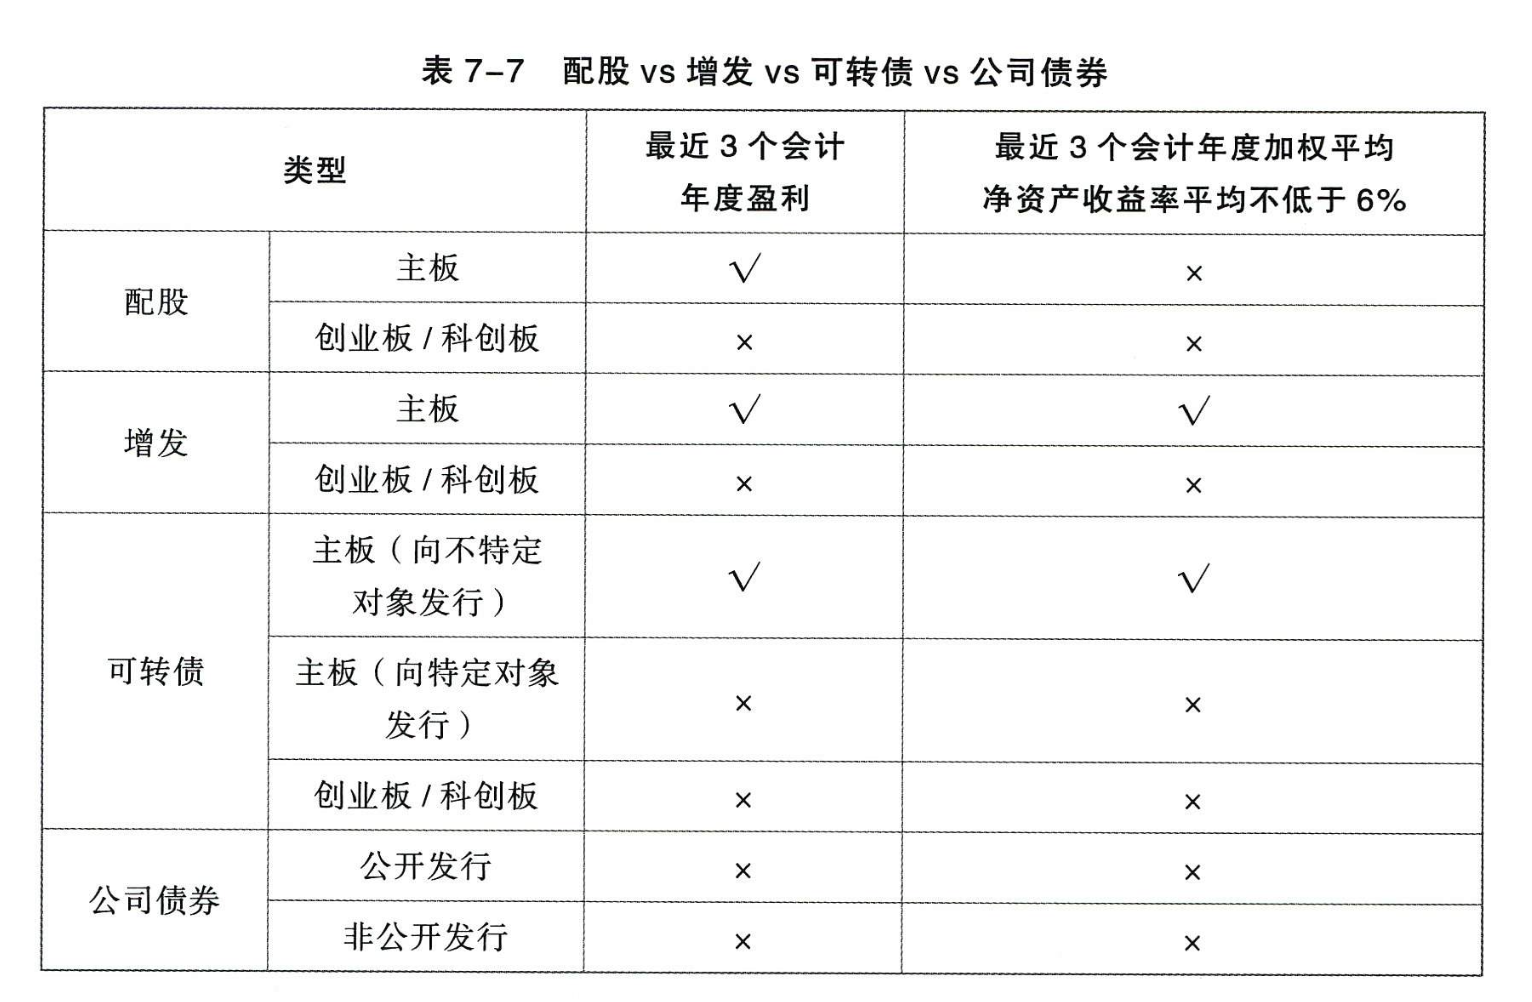
\includegraphics[width=0.7\linewidth]{screenshot001}
		\caption{}
		\label{fig:screenshot001}
	\end{figure}
	
	
	\begin{figure}
		\centering
		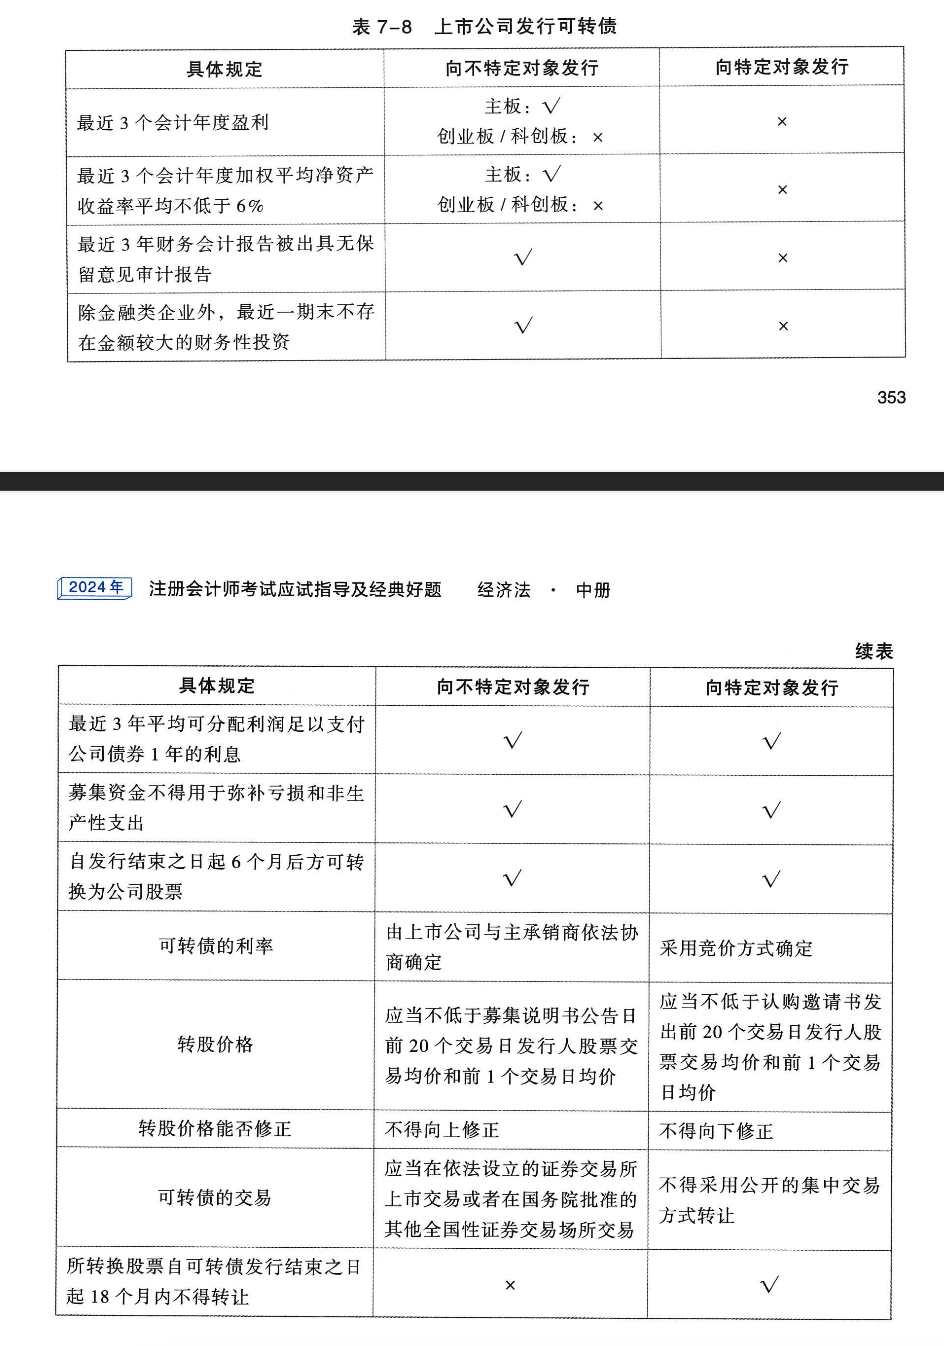
\includegraphics[width=0.7\linewidth]{screenshot002}
		\caption{}
		\label{fig:screenshot002}
	\end{figure}
	
	
	\subsection{上市公司收购}
	\subsubsection{收购人}
	收购是为了取得控制权,以下情形之一视为取得控制权
	\begin{enumerate}
		\item 持股50\%
		
		\item 股份表决权超过30\%
		
		\item 表决权能够决定董事会半数以上成员选任
		
		\item 可以对股东会的决议产生重大影响
		
		\item 中国证监会认定的其他情形
	\end{enumerate}
	
	对收购人的限制如下
	\begin{enumerate}
		\item 收购人有数额较大债务,到期未清偿,且处于持续状态
		
		\item 收购人最近3年有重大违法行为或涉嫌有重大违法行为
		
		\item 收购人最近3年有严重的证券市场失信行为
		
		\item 收购人为自然人,且为不得担任董监高的情形
	\end{enumerate}
	
	控制中还需要关注的一点是一致行动人的界定。其中值得注意的是持有投资者30\%以上股份的自然人和投资人是一致行动人(股份30\%)
	
	\subsubsection{权益变动披露}
	在不同收购情形下进行不同的披露。
	
	首先是场内交易,第一次达到5\%要在该事实发生3日内公告并停止交易(N+3)。后续每次增减5\%都要在该事实发生3日内公告,但停止交易市场要在原基础上增加3日
	
	违反上述规定在买入36月后不得行使股份的表决权。此外,5\%后续每增加1\%都要在次日内通知上市公司并公告。
	
	协议收购类似,如果协议中拟转让的股份达到或者超过5\%,应当在协议达成日起3日内履行权益报告义务
	
	\subsubsection{权益披露的内容}
	披露内容分为两种:简式和详式。两种的选择主要取决于两个因素,如果投资者不是第一大股东或实控人以及拥有的权益数量小于20\%则使用简式,其余都用详式。
	
	简式中包含的内容重点关注投资者及其一致行动人的信息,是否有意在未来12个月内继续增加起在上市公司中拥有的权益
	
	详式在简式的基础上还需要包括
	\begin{enumerate}
		\item 未来12个月内对上市公司资产、业务、人员、组织结构、公司章程等进行调整的后续计划
		
		\item 前24个月内投资者及其一致行动人与上市公司之间的重大交易
	\end{enumerate}
	
	\subsubsection{全面要约还是部分要约}
	如果收购达到发行股份的30\%,继续增持需要采用要约方式
	
	全面需要100\%,部分要约要5\%以上。
	
	如果在协议收购中一次性超过30\%,收购人应当在30日内将股份减少到30以下,否则强制施行全面要约收购义务
	
	\subsubsection{免于发出要约}
	免于发出要约有两种形式,一种是免于发出要约增持,另一种就是免于发出要约。
	
	以下情况下免于发出要约增持
	\begin{enumerate}
		\item 能够证明转让未实现实控人变化
		
		\item 上市公司面临严重财务困难,收购人提出的挽救公司的重组方案取得该公司股东会批准,且收购人承诺3年内不转让起在该公司中所拥有的权益
	\end{enumerate}
	
	免于发出要约的情况都是不想自己增持的情况。
	
	\subsubsection{要约收购}
	要约收购不得小于5\%。约定的收购期在30-60日之间,在收购要约确定的承诺期限内,收购人不得撤销其收购要约
	
	要约期间15日前不得变更收购要约。且变更收购要约只能进行不利变更。
	
	要约价格不得低于要约收购提示性公告前6个月内收购人取得该种股票所支付的最高价格
	
	
	
	\subsubsection{协议收购}
	以协议方式进行上市公司收购的,自签订收购协议起至相关股份完成过户的期间未上市公司收购过渡期。在过渡期内
	\begin{enumerate}
		\item 改选董事会不得超过1/3
		
		\item 被收购公司不得为收购人及其关联方提供担保
		
		\item 被收购同事不得公开发行股份募集资金,不得进行重大购买、出售资产及重大投资行为或者与收购人及其关联方进行其他关联交易,但收购人为挽救陷入危机或者面临严重财务困难的上市公司的情形除外
	\end{enumerate}
	
	\subsubsection{管理层收购}
	不重要。
	
	LBO需要董事会中独立董事超过1/2,且经2/3以上独立董事同意,出席股东会的非关联股东所持表决权过1/2
	
	\subsection{上市公司重大资产重组}
	上市公司重大重组是指上市公司去买别的公司
	
	\subsubsection{重大资产重组行为的界定}
	重大资产重组主要指的就是购买、出售资产或者其他方式进行资产交易达到规定标准,其他方式主要包含
	\begin{enumerate}
		\item 与他人新设企业、对已设立的企业增资或减资
		
		\item 接受经营、租赁其他企业资产或将经营性资产委托他人经营、租赁
		
		\item 接受附义务的资产赠与或者对外捐赠资产
		
		\item 证监会规定的其他情形
	\end{enumerate}
	
	标准主要指
	\begin{enumerate}
		\item 占资产总额的50\%以上
		
		\item 占营业收入的50\%以上且超过5000万人民币
		
		\item 资产净额占净资产的50\%以上且超过5000万人民币
	\end{enumerate}
	
	购买的资产计算选以下二者中较高者
	\begin{enumerate}
		\item 成交金额
		
		\item 被投资企业的资产总额乘以股权比例
	\end{enumerate}
	如果是出售资产的,则与成交金额无关。
	
	同时购买、出售资产的应当分别计算并以较高者为准。12个月内连续进行购买、出售的进行累计计算。
	
	\subsubsection{借壳上市}
	1. 特殊重大资产重组(借壳上市)的界定标准
	上市公司自控制权发生变更之日起36 个月内,向收购人及其关联人购买资产,导致上 市公司发生以下根本变化情形之 一的,构成重大资产重组,应当按照规定履行相关义务和 程序:
	(1 )购买的资产 总额占 上市公司控制权发生变更的前 一个会计年度经审计的合并财务会计
	报告期末资产总额的比例达到 10 0% 以 上;
	(2)购买的资产在最近 一个会计年度所产生的营业收人占上市公司控制权发生变更的前一 个会计年度经审计的合并财务会计报告营业收人的比例达到100% 以上;
	( 3 ) 购 买 的 资 产 净 额 占 上 市 公 司 控 制 权 发 生 变 更 的 前 一个 会 计 年 度 经 审 计 的 合 并 财 务 会 计 报告期末净资产额的比例达到 100% 以 上;
	(4 )为购买资产发行的股份占上市公司首次向收购人及其关联人购买资产的董事会决议前 一个 交 易 日 的 股 份 的 比 例 达 到 1 0 0 % 以 上 ;
	(5 ) 上 市 公 司 向 收 购 人 及 其 关 联 人 购 买 资 产 虽 未 达 到 上 述 第 (1 ) 至 第 ( 4 ) 项 标 准 , 但 可 能导致上市公司主营业务发生根本变化。
	
	借壳上市的最关键问题,是上市公司的控制权发生了变更。上市公司发行股份 购买资产,不 一定导致上市公司的控制权发生变更。如果因发行股份购买资产导致上市公 司的控制权发生了变更 ,则应同时满足发行股份购买资产和借壳上市的相关规定 
	
	上市公司实施特殊重大资产重组(借壳上市),还应当符合下列要求:
	(1 )上市公司购买的资产对应的经营实体应当是股份有限公司或者有限责任公司,且符合 《首次公开发行股票注册管理办法》规定的其他发行条件 、相关板块定位,以及证券交易所规 定的具体条件。
	(2 )上市公司及其量近3 年内的控股股东、实际控制人不存在因涉嫌犯罪正被司法机关立 案侦查或者涉嫌违法违规正被中国证监会立案调查的情形。但是,涉嫌犯罪或者违法违规的行 为已经终止满 3年,交易方案能够消除该行为可能造成的不良后果,且不影响对相关行为人追 究责任的除外。
	(3)上市公司及其控股股东、实际控制人最近12 个月内未受到证券交易所公开谴责,不 存在其他重大失信行为。
	
	\subsubsection{发行股份购买资产}
	1. 发行股份购买资产的基本要求
	(1 )充分说明并披露本次交易有利于提高上市公司资产质量、改善财务状况和增强持续经 营能力,有利于上市公司减少关联交易、避免同业竞争、增强独立性。
	(2 )上市公司最近一年及一期财务会计报告被会计师事务所出具无保留意见的审计报告; 被出具保留意见、否定意见或者无法表示意见的审计报告的,须经会计师事务所专项核查确认, 该保留意见、否定意见或者无法表示意见所涉及事项的重大影响已经消除或者将通过本次交易 予以消除。
	(3 )上市公司及其现任董事、高级管理人员不存在因涉嫌犯罪正被司法机关立案侦查或者涉 嫌违法违规正被中国证监会立案调查的情形;但是,涉嫌犯罪或者违法违规的行为已经终止满3 年,交易方案有助于消除该行为可能造成的不良后果,且不影响对相关行为人追究责任的除外。 (4 )充分说明并披露上市公司发行股份所购买的资产为权属清晰的经营性资产,并能在约 定期限内办理完毕权属转移手续。
	
	
	% \usepackage{tabularray}
	\begin{table}[h!]
		\centering
		\begin{tblr}{
				width = \linewidth,
				colspec = {Q[106]Q[423]Q[412]},
				hlines,
				vlines,
			}
			& 向特定对象发行股票                                                        & 发行股票购买资产                                                               \\
			发行价格        & 发行价不低于定价基准日前20个交易日公司股票均价的80\%                                    & 发行价不低于市场参考价的80\%                                                       \\
			定价基准日/市场参考价 & 定价基准日一般为本次发行股票的 发行期首日,特殊情况下可以为关 于本次发行股票的董事会决议公告日、股东会决议公告日或者发行期首日 & 	市场参考价为本次发行股份购买资产 的董事会决议公告日前20 个交易日、 参考价60 个交易日或者120 个交易日的公  司股票交易均价之一 \\
			锁定期         & 6/18个月                                                           & 一般12/36个月;借壳上市24/36个月                                                  
		\end{tblr}
	\end{table}
	
	
	\subsubsection{公司决议}
	上市公司股东会就重大资产重组事项作出决议,必须经出席会议的股东所持表决权的 2/ 3以上通过。(2022年案例分析题)
	
	上市公司重大资产重组事宜与本公司股东或者其关联人存在关联关系的 ,股东会就重大资产重组事项进行表决时,关联股东应当回避表决。可能导致上市公司的实际控制权发生变化的,上市公司控股股东及其关联人应当回避表决。
	
	除上市公司的董事、监事、高级管理人员、单独或者合计持有上市公司5\%以上股份的股东外,其他股东的投票情况应当单独统计并予以披露。
	
	上市公司就重大资产重组事宜召开股东会,应当以现场会议形式召开,并应当提供网 络投票和其他合法方式为股东参加股东会提供便利。
	
	
	\subsection{强制信息披露制度}
	
	\subsubsection{信息披露的概念和分类}
	1. 信息披露义务人 信息披露义务人包括:上市公司及其董事、监事、高级管理人员、股东、实际控制人,收 购人,重大资产重组、再融资、重大交易有关各方等自然人、单位及其相关人员,破产管理人 及其成员,以及法律、行政法规和中国证监会规定的其他承担信息披露义务的主体。
	2. 强制信息披露和自愿信息披露 以披露的信息内容是否为法律强制规定必须公开的内容为标准,信息披露可以分为强制信 息披露和自愿信息披露 。强制信息披露规范 主要适用 于公开发行的证券。
	3. 自愿披露的信息(2022年案例分析题)
	(1)除依法需要披露的信息之外 ,信息披露义务人可以自愿披露与投资者作出价值判断和 投资决策有关的信息,但不得与依法披露的信息相冲突,不得误导投资者。 (2)信息披露义务人自愿披露的信息应当真实、准确、完整 。自愿性信息披露应当遵守公 平原则,保持信息披露的持续性和 一致性,不得进行选择性披露。
	(3 )信息披露义务人不得利用自愿披露的信息不当影响公司证券及其衍生品种交易价格, 不得利用自愿性信息披露从事市场操纵等违法违规行为。
	【解释】发行人一旦自愿选择披露依法需披露的信息之外的信息,则应采用与强制信 息披露同样的披露原则,例如真实、准确、完整等原则,如果在自愿披露的内容中出现虛 假陈述,也要承担相应的民事赔偿责任。
	
	4. 客观信息的披露和主观信息的披露
	(1 )以信息披露的内容为标准,信息披露可以分为客观信息的披露和主观信息的披露。 (2 )客观信息的披露,即 “ 硬信息” 、历史性信息的披露,是指发行人、上市公司将其 已 经发生的相关事实(如上市公司的经营状况、财务报告等)依法进行披露。 (3)主观信息的披露,即 “软信息”、预测性信息的披露,是指发行人、上市公司对公司 未来经营情况、财务状况进行判断并公布, 一般表现为盈利预测和管理层讨论和分析。虚假陈 述一般发生在“硬信息” 披露环节,但需要强调的是,预测性信息披露有可能因未进行充分风 险提示、预测无依据等情形构成虚假陈述。
	5. 首次信息披露和持续信息披露
	(1 )以信息披露的发生阶段为标准,信息披露可以分为首次信息披露和持续信息披露。
	(2 )首次信息披露的法定文件主要是招股说明书和债券募集说明书。上市公告书虽不属于 发行信息披露文件,但作为公司上市首次披露的文件,也可将其界定为首次信息披露的范畴。 (3 )持续信息披露主要有定期报告和临时报告。上市公司应当披露的定期报告包括年度报 告、中期报告。
	【解释】季度报告不属于强制信息披露的范围。
	
	6. 招股说明书(2024年调整) (1)招股说明书是公开发行股票最基本的法律文件。发行人首次公开发行股票的信息主要 是通过招股说明书披露。
	(2 )招股说明书内容与格式准则是信息披露的最低要求。不论准则是否有明确规定,凡是 对投资者作出投资决策有重大影响的信息,均应当予以披露。发行人应当在招股说明书中披露
	已达到发行监管对公司独立性的基本要求。
	(3 )招股说明书的有效期为6 个月,自公开发行前最后一次签署之日起计算。招股说明书 中引用经审计的财务报表在其最近一期截止日后6 个月内有效,特 情况下发行人可申请适当 延长,但至多不超过3 个月。财务报表应当以年度末、半年度末或者季度末为截止日。 (4)发行人及其董事、监事和高级管理人员应当在招股说明书上签署书面确认意见,保证 招股说明书的内容真实、准确、完整,不存在虚假记载、误导性陈述或者重大遗漏,按照诚信 原则履行承诺,并声明承担相应法律责任。
	(5 )保荐人及其保荐代表人,以及发行人控股股东、实际控制人应当在招股说明书上签字、 盖章,确认招股说明书的内容真实、准确、完整,不存在虚假记载、误导性陈述或者重大遗漏, 按照诚信原则履行承诺,并声明承担相应法律责任。
	(6 )保荐人出具的发行保荐书、证券服务机构出具的文件以及其他与发行有关的重要文件 应当作为招股说明书的附件。
	(7 )证券交易所受理注册申请文件后,发行人应当按规定,将招股说明 书、发行保荐书、 上市保荐书、审计报告和法律意见书等文件在交易所网站预先披露。预先披露的招股说明书及 其他注册申请文件不能含有价格信息,发行人不得据此发行股票。
	
	\subsubsection{定期报告}
	1. 披露时间 上市公司、公司债券上市交易的公司、股票在全国中小企业股份转让系统交易的公司,应当 按照中国证监会和证券交易场所规定的内容和格式编制定期报告,并按照以下规定报送和公告:
	
	(1 )年 度 报 告 在每一会计年度结束之日起4个月内,报送并公告年度报告,其中的年度财务会计报告应 当经符合《证券法》规定的会计师事务所审计。定期报告中财务会计报告被出具非标准审计意 见的,上市公司董事会应当针对该审计意见涉及事项作出专项说明。
	(2 )中期报告
	在每一会计年度的上半年结束之日起2 个月内,报送并公告中期报告。
	
	\subsubsection{临时报告}
	1. 股票
	根据《证券法》第80 条的规定,发生可能对上市公司、股票在国务院批准的其他全国性 证券交易场所交易的公司的股票交易价格产生较大影响的重大事件,投资者尚未得知时,公司 应当立即将有关该重大事件的情况向国务院证券监督管理机构和证券交易场所报送临时报告, 并子公告,说明事件的起因、目前的状态和可能产生的法律后果。其中的重大事件包括:
	(1 )公司的经营方针和经营范围的重大变化; (2)公司的重大投资行为,公司在1年内购买、出售重大资产超过公司资产总额30%, 或者公司营业用主要资产的抵押、质押、出售或者报废 一次超过该资产的30%;
	(3 )公司订立重要合同、提供重大担保或者从事关联交易,可能对公司的资产、负债、权 益和经营成果产生重要影响;
	(4 )公司发生重大债务和未能清偿到期重大债务的违约情况;
	(5 )公司发生重大亏损或者重大损失;
	(6 )公司生产经营的外部条件发生的重大变化;
	(7 ) 公 司 的 董 事 、 1 / 3 以 上 监 事 或 者 经 理 发 生 变 动 , 董 事 长 或 者 经 理 无 法 履 行 职 责 ;
	【 解 释 】( 1 ) 任 何 一 个 董 事 发 生 变 动 均 属 于 重 大 事 件 , 不 受 1 / 3 的 数 量 限 制 ;( 2 ) 总 经 理 (不包括副经理、财务负责人)发生变动,才属于重大事件
	
	(8 )持有公司5%以上股份的股东或者实际控制人持有股份或者控制公司的情况发生较大 变化,公司的实际控制人及其控制的其他企业从事与公司相同或者相似业务的情况发生较大 变化; (9)公司分配股利、增资的计划,公司股权结构的重要变化,公司减资、合并、分立、解 散及申请破产的决定,或者依法进入破产程序、被责令关闭; (10)涉及公司的重大诉讼、仲裁,股东会、董事会决议被依法撤销或者宣告无效; (11)公司涉嫌犯罪被依法立案调查,公司的控股股东、实际控制人、董事、监事、高级 管理人员涉嫌犯罪被依法采取强制措施;
	(12 )国务院证券监督管理机构规定的其他事项。
	【解释1】持有上市公司5%以上股份的股东或者实际控制人,其持有股份或者控制公 司的情况发生较大变化的,应当主动告知上市公司董事会,并配合上市公司履行信息披露 义务。
	【解释2 】公司的控股股东或者实际控制人对重大事件的发生、进展产生较大影响的, 应当及时将其知悉的有关情况书面告知公司,并配合公司履行信息披露义务。
	【解释3 】上市公司控股子公司发生重大事件,可能对上市公司证券及其衍生品种交易 价格产生较大影响的,上市公司应当履行信息披露义务。(2022 年案例分析題) 【解释4】上市公司披露重大事件后 ,已披露的重大事件出现可能对上市公司证券及其 衍生品种交易价格产生较大影响的进展或者变化的,应当及时披露进展或者变化情况、可 能产生的影响。(2022 年案例分析题)
	
	2. 公司债券
	根据《证券法》第81 条的规定,发生可能对上市交易公司债券的交易价格产生较大影响 的重大事件,投资者尚未得知时,公司应当立即将有关该重大事件的情况向国务院证券监督管 理机构和证券交易场所报送临时报告,并予公告,说明事件的起因、目前的状态和可能产生的 法律后果。其中的重大事件包括:
	(1)公司股权结构或者生产经营状况发生重大变化;
	(2 )公司债券信用评级发生变化;
	(3 )公司重大资产抵押、质押、出售、转让、报废;
	(4 ) 公 司 发 生 未 能 清 偿 到 期 债 务 的 情 况 ;
	(5 )公司新增借款或者对外提供担保超过上年末净资产的 20%;
	(6 ) 公 司 放 弃 债 权 或 者 财 产 超 过 上 年 末 净 资 产 的 1 0 % ;
	(7 ) 公 司 发 生 超 过 上 年 末 净 资 产 1 0 % 的 重 大 损 失 ;
	(8 )公司分配股利 ,作出减资、合并、分立、解散及申请破产的决定,或者依法进入破产 程序、被责令关闭;
	(9 )涉及公司的重大诉讼、仲裁;
	(10 )公司涉嫌犯罪被依法立案调查,公司的控股股东、实际控制人、董事、监事、高级 管理人员涉嫌犯罪被依法采取强制措施;
	(11)国务院证券监督管理机构规定的其他事项。
	
	【解释】根据 《公司债券发行与交易管理办法》的规定,募投项目情况发生重大变化, 可能影响募集资金投入和使用计划,或者导致项目预期运营收益实现存在较大不确定性, 也 属 于 重 大 事 件 。 (2 0 2 4 年 新 增 )
	3. 重大事件的披露(2019年案例分析题、2022年案例分析题、2023年案例分析题) 上市公司应当在最先发生的以下任 一时点,及时履行重大事件的信息披露义务: (1)董事会或者监事会就该重大事件形成决议时;
	(2 )有关各方就该重大事件签署意向书或者协议时; (3)董事、监事或者高级管理人员知悉该重大事件发生时。
	【解释】“及时” 是指自起算日起或者触及披露时点的2个交易日内。在上述规定的时 点 之前出现 下列情形 之一的, 上市公司应 当及时披露相关事项的现 状、 可能影响事件进 展的风险因素:(1 )该重大事件难以保密;(2 )该重大事件已经泄露或者市场出现传闹; (3 )公司证券及其衍生品种出现异常交易情况。
	
	\subsubsection{信息披露的事务管理}
	1. 上市公司信息披露的制度化管理 (1)上市公司应当制定定期报告的编制、审议、披露程序。经理、财务负责人、董事会秘 书等高级管理人员应当及时编制定期报告草案,提请董事会审议;董事会秘书负责送达董事审 阅;董事长负责召集和主持董事会会议审议定期报告;监事会负责审核董事会编制的定期报告; 董事会秘书负责组织定期报告的披露工作。
	( 2 ) 上 市 公 司 应 当 制 定 重 大 事 件 的 报 告 、 传 递 、 审 核 、 披 露 程 序 。 董 事 、 监 事 、高 级 管 理 人员知悉重大事件发生时,应当按照公司规定立即履行报告义务;董事长在接到报告后,应当 立即向董事会报告,并敦促董事会秘书组织临时报告的披露工作。
	
	(3 )上市公司董事、监事、高级管理人员、持股5%以上的股东及其 一致行动人、实际控 制人应当及时向上市公司董事会报送上市公司关联人名单及关联关系的说明。上市公司应当履 行关联交易的审议程序,并严格执行关联交易回避表决制度。交易各方不得通过隐瞒关联关系 或者采取其他手段,规避上市公司的关联交易审议程序和信息披露义务。
	2. 上市公司及其他信息披露义务人在信息披露工作中的职责
	(1 )信息披露义务人应当及时依法履行信息披露义务,披露的信息应当真实、准确、完整, 简明清晰、通俗易懂,不得有虚假记载、误导性陈述或者重大遗漏。
	(2 )信息披露义务人披露的信息应当同时向所有投资者披露,不得提前向任何单位和个人 泄繹。但是,法律、行政法规另有规定的除外。
	(3 )在内幕信息依法披露前,内幕信息的知情人和非法获取内幕信息的人不得公开或者泄 露该信息,不得利用该信息进行内幕交易 。任何单位和个人不得非法要求信息披露义务人提供 依法需要披簬但尚未披簬的信息。
	(4 )证券及其衍生品种同时在境内境外公开发行、交易的,其信息披露义务人在境外市场 披露的信息,应当同时在境内市场披露。
	(5 )上市公司通过业绩说明会、分析师会议、路演、接受投资者调研等形式就公司的经营 情况、财务状况及其他事件与任何单位和个人进行沟通的,不得提供内幕信息。
	(6 )信息披露义务人不得以新闻发布或者答记者问等任何形式代替应当履行的报告、公告 义务,不得以定期报告形式代替应当履行的临时报告义务。(2023 年案例分析题)
	3. 上市公司的董事、监事、高级管理人员在信息披露工作中的职责 (1)上市公司的董事、监事、高级管理人员应当忠实、勤勉地履行职责,保证披露信息的 真实、准确、完整 ,信息披露及时、公平。 (2)董事应当了解并持续关注公司生产经营情况、财务状况和公司已经发生的或者可能发 生的重大事件及其影响,主动调查、获取决策所需要的资料。 (3)监事应当对公司董事、高级管理人员履行信息披露职责的行为进行监督;关注公司信 息披露情况,发现信息披露存在违法违规问题的,应当进行调查并提出处理建议。
	(4 )高级管理人员应当及时向董事会报告有关公司经营或者财务方面出现的重大事件、已 披露的事件的进展或者变化情况及其他相关信息。
	(5 )董事会秘书负责组织和协调公司信息披露事务,汇集上市公司应予披露的信息并报告 董事会,持续关注媒体对公司的报道并主动求证报道的真实情况。董事会秘书负责办理上市公 司信息对外公布等相关事宜。
	(6 )上市公司董事、监事、高级管理人员应当对公司信息披露的真实性、准确性、完整性、 及时性、公平性负责,但有充分证据表明其已经履行勤勉尽责义务的除外。 (7)上市公司董事长、经理 、董事会秘书,应当对公司临时报告信息披露的真实性、准确 性、完整性、及时性 、公平性承担主要责任。
	(8)上市公司董事长 、经理、财务负责人应当对公司财务会计报告的真实性、准确性、完 整性、及时性 、公平性承担主要责任。
	
	
	4. 上市公司的股东、实际控制人在信息披露工作中的职责 (1)上市公司的股东、实际控制人发生以下事件时,应当主动告知上市公司董事会,并配 合上市公司履行信息披露义务:
	1持有公司5% 以 上股份的股东或者实际控制人持有股份或者控制公司的情况发生较 大变 化,公司的实际控制人及其控制的其他企业从事与公司相同或者相似业务的情况发生较大变化; 2法院裁决禁止控股股东转让其所持股份,任 一股东所持公司5%以上股份被质押、冻结、 司法拍卖、托管、设定信托或者被依法限制表决权等,或者出现被强制过户风险; 3拟对上市公司进行重大资产或者业务重组;
	4中国证监会规定的其他情形。
	(2 )应当披簬的信息依法披露前,相关信息已在媒体上传播或者公司证券及其衍生品种出 现交易异常情况的,股东或者实际控制人应当及时、准确地向上市公司作出书面报告,并配合 上市公司及时、准确地公告。(2020 年案例分析题) (3)上市公司的股东、实际控制人不得滥用其股东权利、支配地位,不得要求上市公司向 其提供内幕信息。
	(4 )上市公司向特定对象发行股票时,其控股股东、实际控制人和发行对象应当及时向上 市公司提供相关信息,配合上市公司履行信息披露义务。
	(5 )通过接受委托或者信托等方式持有上市公司5%以上股份的股东或者实际控制人,应 当及时将委托人情况告知上市公司,配合上市公司履行信息披露义务。
	5. 证券服务机构在信息披露工作中的职责
	(1 )为信息披露义务人履行信息披露义务出具专项文件的证券公司、证券服务机构及其人 员,应当勤勉尽责、诚实守信,按照法律、行政法规、中国证监会规定、行业规范、业务规则 等发表专业意见,保证所出具文件的真实性、准确性和完整性。
	(2 )证券公司、证券服务机构在为信息披露出具专项文件时,发现上市公司及其他信息披 露义务人提供的材料有虚假记载、误导性陈述、重大遗漏或者其他重大违法行为的,应当要求 其补充、纠正。
	(3 )证券服务机构应当妥善保存客户委托文件、核查和验证资料、工作底稿以及与质量控 制、内部管理、业务经营有关的信息和资料。证券服务机构应当配合中国证监会的监督管理, 在规定的期限内提供、报送或者披露相关资料、信息,保证其提供、报送或者披露的资料、信 息真实、准确、完整,不得有虚假记载、误导性陈述或者重大遗漏。
	(4 )会计师事务所应当建立并保持有效的质量控制体系、独立性管理和投资者保护机制, 秉承风险导向审计理念,遵守法律、行政法规、中国证监会的规定,严格执行注册会计师执业 准则、职业道德守则及相关规定,完善鉴证程序,科学选用鉴证方法和技术,充分了解被鉴证 单位及其环境,审慎关注重大错报风险,获取充分、适当的证据,合理发表鉴证结论。
	
	\subsection{内幕交易}
	内幕交易和虚假陈述都为证券违法行为
	
	\subsubsection{内幕信息}
	内幕信息就是涉及发行人的尚未公开的真信息
	
	3. 内幕信息的敏感期
	(1)内幕信息的 一个重要特征是 “尚未公开”。内幕交易只能发生在内幕信息形成至公开 之间的这段时期内,这段时期被称为“内幕信息的敏感期”。
	(2 )内 幕 信 息 的 形 成 (2 0 1 8 年 案 例 分 析 题 、 2 0 1 9 年 案 例 分 析 题 )
	根 据 《内 幕 交 易 案 件 若 干问 题 解 释 》 的 规 定 : 1 《证 券 法 》 第 8 0 条 、 第 8 1 条 所 列 “ 重 大 事件” 的发生时间,“重大事件” 中涉及的“计划” “方案” 等的形成时间,应当认定为内幕信 息的形成之时;2影响内幕信息形成的动议、筹划、决策或者执行人员,其动议、筹划、决策 或者执行初始时间,应当认定为内幕信息的形成之时。
	(3 )内幕信息的公开 内幕信息的公开,是指内幕信息在国务院证券、期货监督管理机构指定的报刊、网站等媒 体披露。
	
	\subsubsection{内幕交易行为}
	1. 证券交易内幕信息的知情人
	(1 )发行人及其董事、监事、高级管理人员;
	(2 ) 持 有 公 司 5 % 以 上 股 份 的 股 东 及 其 董 事 、 监 事 、 高 级 管 理 人 员 , 公 司 的 实 际 控 制 人 及 其董事、监事、高级管理人员;
	(3 )发行人控股或者实际控制的公司及其董事、监事、高级管理人员;
	(4 ) 由 于所 任 公 司 职 务 或 者 因 与 公 司 业 务 往 来 可 以 获 取 公 司 有 关 内 幕 信 息 的 人 员 ;
	(5 )上市公司收购人或者重大资产交易方及其控股股东、实际控制人、董事、监事和高级 管理人员;
	(6 )因职务、工作可以获取内幕信息的证券交易场所、证券公司、证券登记结算机构、证 券服务机构的有关人员; (7)因职责、工作可以获取内幕信息的证券监督管理机构工作人员;
	(8 )因法定职责对证券的发行、交易或者对 上市公司及其收购、重大资产交易进行管理可 以获取内幕信息的有关主管部门、监管机构的工作人员;
	(9 )国务院证券监督管理机构规定的可以获取内幕信息的其他人员。
	2. 非法获取证券内幕信息的人员
	(1 )利用窃取、骗取、套取、窃听、利诱、刺探或者私下交易等 手段获取内幕信息的。 (2 )内幕信息知情人员的近亲属或者其他与内幕信息知情人员关系密切的人员,在内幕信 息敏感期内,从事或者明示、暗示他人从事,或者泄露内幕信息导致他人从事与该内幕信息有 关的证券、期货交易,相关交易行为明显异常,且无正当理由或者正当信息来源的。
	(3 )在内幕信息敏感期内,与内幕信息知情人员联络、接触,从事或者明示、暗示他人从 事,或者泄露内幕信息导致他人从事与该内幕信息有关的证券、期货交易,相关交易行为明显 异常,且无正当理由或者正当信息来源的。
	3. 内幕交易行为的推定(2018 年案例分析题、2019 年案例分析题、2020 年案例分析题、 2022 年案例分析题 )
	只要监管机构提供的证据能够证明以下情形之 一,就可以推定内幕交易行为成立:
	(1 )证券交易内幕信息知情人员,进行了与该内幕信息有关的证券交易活动;
	(2 ) 内 幕 信 息 知 情 人 员 的 配 偶 、 父 母 、 子 女 以 及 其 他 有 密 切 关 系 的 人 , 其 证 券 交 易 活 动 与 该内幕信息基本吻合;
	(3 )因履行工作职责知悉上述内幕信息并进行了与该信息有关的证券交易活动;
	(4 )非法获取内幕信息,并进行 了与该内幕信息有关的证券交易活动;
	(5 )内幕信息公开前与内幕信息知情人员或者知晓该内幕信息的人员联络、接触,其证券 交易活动与内幕信息高度吻合。
	【解释】当事人可以通过举证推翻上述推定。当事人可以对其在内幕信息敏感期内从 事的相关证券交易活动作出合理说明,或者提供证据排 除其存在利用内幕信息从事相关证 券 交 易 活 动 的 可 能 。 (2 0 2 4 年 调 整 )
	
	4. 不构成“内幕交易罪” 的情形(2019年案例分析题)
	(1 )持有或者通过协议、其他安排与他人共同持有 上市公司5 % 以 上股份的自然人、法人 或者其他组织收购该 上市公司股份的;
	(2 )按照事先订立的书面合同、指令、计划从事相关证券、期货交易的;
	(3 )依据已被他人披露的信息而交易的;
	(4 )交易具有其他正当理由或者正当信息来源的。
	
	5. 利用内幕信息以外的其他未公开信息进行的交易(2020年案例分析题) 禁止证券交易场所、证券公司、证券登记结算机构、证券服务机构和其他金融机构的从业 人员、有关监管部门或者行业协会的工作人员,利用因职务便利获取的内幕信息以外的其他未 公开的信息,违反规定,从事与该信息相关的证券交易活动,或者明示、暗示他人从事相关交 易活动。
	【解释】上述行为俗称“老鼠仓” 行为。“老鼠仓” 行为与内幕交易行为的主要区别: (1)主体范围不同。“老鼠仓” 行沟的主体特定,主要是证券交易场所、证券公司、证券 登记结算机构、证券服务机构和其他金融机构的从业人员、有关监管部门或者行业协会的 工作人员;而内幕交易的主体不仅包括证券交易内幕信息的知情人员,还包括非法获取内 幕信息的人员;(2)所利用的信息不同。“老鼠仓” 行为利用的是内幕信息以外的其他未 公开的信息;而内幕交易利用的是内幕信息(涉及发行人经营、财务的具有重大性且未公 开的信息)。
	
	\subsubsection{短线交易}
	1. 上市公司、股票在国务院批准的其他全国性证券交易场所交易的公司持有5%以上股份 的股东 、董事、监事、高级管理人员,将其持有的该公司的股票或者其他具有股权性质的证券 在买人后6 个月内卖出,或者在卖出后6 个月内又买人,由此所得收益归该公司所有,公司董 事会应当收回其所得收益。但是,证券公司因购人包销售后剩余股票而持有5%以上股份,以 及有国务院证券监督管理机构规定的其他情形的除外。上述董事、监事、高级管理人员、自然 人股东持有的股票或者其他具有股权性质的证券,包括其配偶、父母、子女持有的及利用他人 账户持有的股票或者其他具有股权性质的证券。
	2. 公司董事会不按规定执行的,股东有权要求董事会在30日内执行。公司董事会未在上 述期限内执行的,股东有权为了公司的利益以自己的名义直接向人民法院提起诉讼。公司董事 会不按规定执行的,负有责任的董事依法承担连带责任。
	【解释】根据2024 年教材的观点,对于提起诉讼的股东,没有持股比例(1%)和特 股期限(180 日)的限制,也不涉及先找董事会或者监事会的程序问题。
	
	
	\subsubsection{股份转让的限制}
	1. 公司公开发行股份前已发行的股份,自公司股票在证券交易所上市交易之日起1年内 不得转让。
	2. 董事、监事、高级管理人员 (1)董事、监事、高级管理人员所持本公司股份,自公司股票上市交易之日起1 年内不得 转让。 (2)董事、监事、高级管理人员在任职期间每年转让的股份不得超过其所持有本公司股份 总数的25%。
	(3)董事、监事、高级管理人员离职后6 个月内,不得转让其所持有的本公司股份。
	
	(4 )上市公司董事、监事和高级管理人员在 下列期间不得买卖本公司股票: 1上市公司年度报告、半年度报告公告前30 日内;
	2 上市公司季度报告、业绩预告、业绩快报公告前 10 日内; 3自可能对本公司证券及其衍生品种交易价格产生较大影响的重大事件发生之日或在决策 过程中,至依法披露之日内。
	3. 短线交易
	上 市 公 司 、 股 票 在 国 务 院 批 准 的 其 他 全 国 性 证 券 交 易 场 所 交 易 的 公 司 持 有 5 % 以 上股 份 的 股东、董事、监事、高级管理人员,将其持有的该公司的股票或者其他具有股权性质的证券在 买人后6 个月内卖出,或者在卖出后6 个月内又买入,由此所得收益归该公司所有,公司董事 会应当收回其所得收益。但是,证券公司因购入包销售后剩余股票而持有5%以上股份,以及 有国务院证券监督管理机构规定的其他情形的除外。
	4. 上市公司向特定对象发行股票
	(1)18 个月
	上市公司董事会决议提前确定全部发行对象,且发行对象属于下列情形之 一的,定价基准 日可以为关于本次发行股票的董事会决议公告日、股东会决议公告日或者发行期首日,认购的 股票自发行结束之日起 18 个月内不得转让:
	1 上市 公 司 的 控 股 股 东 、 实 际 控 制 人 或 其 控 制 的 关联 人 ; 2通过认购本次发行的股票取得上市公司实际控制权的投资者; 3董事会拟引入的境内外战略投资者。
	(2 )6 个 月
	除此之外的发行对象,认购的股票自发行结束之日起6 个月内不得转让。
	5. 上市公司发行股份购买资产 (1)特定对象以资产认购而取得的上市公司股份,自股份发行结束之日起12个月内不得转让。 (2 )属于下列情形之一的,36 个月内不得转让: 1特定对象为上市公司控股股东、实际控制人或者其控制的关联人。 2特定对象通过认购本次发行的股份取得上市公司的实际控制权。 3特定对象取得本次发行的股份时,对其用于认购股份的资产持续拥有权益的时间不足 12 个月。
	(3)上市公司发行股份购买资产,属于“借壳上市” 情形的,上市公司原控股股东、原实 际控制人及其控制的关联人,以及在交易过程中从该等主体直接或者间接受让该上市公司股份 的特定对象应当公开承诺,在本次交易完成后36 个月内不转让其在该上市公司中拥有权益的 股份;除收购人及其关联人以外的特定对象应当公开承诺,其以资产认购而取得的上市公司股 份自股份发行结束之日起2 4 个月内不得转让。
	6. 上市公司的收购人
	收购人持有的被收购的上市公司的股票,在收购行为完成后的18 个月内不得转让。但是, 收购人在被收购公司中拥有权益的股份在同一实际控制人控制的不同主体之间进行转让,不受 18 个月的限制,但应当遵守《上市公司收购管理办法》关于免于发出要约的有关规定。
	7. 上市公司向特定对象发行的可转债转股的,所转换股票自可转债发行结束之日起18个 月内不得转让。
	
	\subsection{虛假陈述}
	
	\subsubsection{虚假陈述行为的界定}
	1. 最高人民法院的《虚假陈述侵权民事赔偿规定》将虚假陈述主要分为虚假记载、误导 性陈述和重大遗漏。
	(1 )虚假记载,是指信息披露义务人披露的信息中对相关财务数据进行重大不实记载,或 者对其他重要信息作出与真实情况不符的描述。 (2)误导性陈述,是指信息披露义务人披露的信息隐瞒了与之相关的部分重要事实,或者 未及时披露相关更正、确认信息,致使已经披露的信息因不完整、不准确而具有误导性。
	(3 )重大遗漏,是指信息披露义务人违反关于信息披露的规定,对重大事件或者重要事项 等应当披露的信息未予披露。
	2 . 预 测 性 信 息 (2 0 2 2 年 案 例 分 析 题 ) 原告以信息披露文件中的盈利预测、发展规划等预测性信息与实际经营情况存在重大差异 为由主张发行人实施虚假陈述的,人民法院不予支持,但有下列情形之一的除外:
	(1 )信 息 披 露 文件 未 对 影 响 该 预 测 实 现 的 重 要 因 素 进 行 充 分 风 险 提 示 的 ;
	(2 )预测性信息所依据的基本假设、选用的会计政策等编制基础明显不合理的;
	(3 )预测性信息所依据的前提发生重大变化时,未及时履行更正义务的。
	
	\subsubsection{虚假陈述行为的行政责任}
	1. 根据中国证监会的《信息披露违法行为行政责任认定规则》,上市公司发生信息披露违 法行为的,对负有保证信息披譯真实、准确、完整、及时和公平义务的董事、监事、高级管理 人员,应当视情形认定其为直接负责的主管人员或者其他直接责任人员承担行政责任,但其能 够证明已尽忠实、勤勉义务,没有过错的除外。
	
	2. 根据《信息披露违法行为行政责任认定规则》,如有证据证明因信息披露义务人受控股 股东、实际控制人指使,未按照规定披露信息,或者所披露的信息有虚假记载、误导性陈述或 者重大遗漏的,在认定信息披露义务人责任的同时,应当认定信息披露义务人控股股东、实际 控制人的信息披露违法责任。信息披露义务人的控股股东、实际控制人是法人的,其负责人应 当认定为直接负责的主管人员。控股股东、实际控制人直接授意、指挥从事信息披露违法行为, 或者隐瞒应当披鰩信息、不告知应当披露信息的,应当认定控股股东、实际控制人指使从事信 息披露违法行为。
	3. 可以考虑“不予行政处罚” 的情形
	(1 )当事人对认定的信息披露违法事项提出具体异议记载 于董事会、监事会、公司办公会 会议记录等,并在上述会议中投反对票(不包括弃权)的;
	(2 )当事人在信息披露违法事实所涉及期间,由于不可抗力、失去人身自由等无法正常履 行职责的;
	(3 )对公司信息披露违法行 不负有主要责任的人员在公司信息披露违法行 发生后及时 向公司和证券交易所、证券监管机构报告的。
	4. 不得单独作为不子处罚情形认定(2022年案例分析题、2023年案例分析题) 《信息披露违法行为行政责任认定规则》明确规定,任何下列情形,不得单独作为不予处 罚情形认定:
	(1 )不直接从事经营管理;
	(2 )能力不足、无相关职业背景;
	(3)任职时间短、不了解情况;
	(4 )相信专业机构或者专业人员出具的意见和报告;
	(5 )受到股东、实际控制人控制或者其他外部干预。
	
	\subsubsection{虚假陈述行为的民事赔偿责任}
	1. 无过错责任 根据《证券法》第85条的规定,信息披露义务人未按照规定披露信息,或者公告的证券 发行文件、定期报告、临时报告及其他信息披露资料存在虚假记载、误导性陈述或者重大遗漏, 致使投资者在证券交易中遭受损失的,信息披露义务人应当承担赔偿责任。
	2 . 过 错 推 定 责 任 (2 0 2 0 年 案 例 分 析 题 )
	(1 )根据 《证券法》第85 条的规定,发行人的控股股东、实际控制人、董事、监事、高 级管理人员和其他直接责任人员以及保荐人、承销的证券公司及其直接责任人员,应当与发行 人承担连带赔偿责任,但是能够证明自己没有过错的除外。 (2)根据《证券法》第163条的规定,证券服务机构为证券的发行、上市、交易等证券业 务活动制作、出具审计报告及其他鉴证报告、资产评估报告、财务顾问报告、资信评级报告或 者法律意见书等文件,应当勤勉尽责,对所依据的文件资料内容的真实性、准确性、完整性进 行核查和验证。其制作、出具的文件有虚假记载、误导性陈述或者重大遗漏,给他人造成损失 的,应当与委托人承担连带赔偿责任,但是能够证明自己没有过错的除外。
	
	% \usepackage{tabularray}
	\begin{table}
		\centering
		\begin{tblr}{
				width = \linewidth,
				colspec = {Q[98]Q[258]Q[583]},
				cell{3}{1} = {r=4}{},
				cell{3}{3} = {r=4}{},
				vlines,
				hline{1-3,7} = {-}{},
				hline{4-6} = {2}{},
			}
			责任类型   & 责任主体               & 具体内容                                          \\
			无过错责任  & 信息披露义务人            & 信息披露义务人只要存在虚假陈述行 为,无论是否有过错,均应承担损害赔 偿责任        \\
			过错推定责任 & 发行人的控股股东、实控人       & 先推定其有过错,原告无需承担举证责任;如果被告不能证明自己没有过错,则应当承担连带赔偿责任 \\
			& 发行人的董监高和其他直接责任人    &                                               \\
			& 保荐人、承销的证券公司及其直接责任人 &                                               \\
			& 证券服务机构             &                                               
		\end{tblr}
	\end{table}
	
	\subsubsection{过错认定}
	1. 过错的认定 根据《虚假陈述侵权民事赔偿规定》,《证券法》第85条、第163条所称的过错,包括以 下两种情形: (1)行为人故意制作、出具存在虚假陈述的信息披露文件,或者明知信息披露文件存在虚 假陈述而不予指明、予以发布;
	(2 )行为人严重违反注意义务,对信息披露文件中虚假陈述的形成或者发布存在过失。
	2. 发行人的董事、监事、高级管理人员(2022年案例分析题) (1)发行人的董事、监事、高级管理人员和其他直接责任人员主张对虚假陈述没有过错的,
	
	人民法院应当根据其工作岗位和职责、在信息披露资料的形成和发布等活动中所起的作用、取 得和了解相关信息的渠道、为核验相关信息所采取的措施等实际情况进行审查认定。
	(2 )上述人员不能提供勤勉尽责的相应证据,仅以其不从事日常经营管理、无相关职业背 景和专业知识、相信发行人或者管理层提供的资料、相信证券服务机构出具的专业意见等理由 主张其没有过错的,人民法院不予支持。
	【相关链接】任何下列情形,不得单独作为不予处罚情形认定:(1)不直接从事经营管 理;(2 )能力不足、无相关职业背景;(3 )任职时间短、不了解情况;(4 )相信专业机构或 者专业人员出具的意见和报告;(5 )受到股东、实际控制人控制或者其他外部 干预。
	(3 )发行人的董事、监事、高级管理人员依照《证券法》的规定,以书面方式发表附具体 理由的意见并依法披露的,人民法院可以认定其主观上没有过错,但在审议、审核信息披露文 件时投赞成票的除外。
	
	3 . 独 立 董 事 (2 0 2 2 年 案 例 分 析 题 )
	独立董事能够证明下列情形之 一的,人民法院应当认定其没有过错: (1)在签署相关信息披露文件之前,对不属于自身专业领域的相关具体问题,借助会计、 法律等专门职业的帮助仍然未能发现问题的;
	(2 )在揭露日或者更正日之前,发现虚假陈述后及时向发行人提出异议并监督整改或者向 证券交易场所、监管部门书面报告的; (3)在独立意见中对虚假陈述事项发表保留意见、反对意见或者无法表示意见并说明具体 理由的,但在审议、审核相关文件时投赞成票的除外;
	(4)因发行人拒绝 、阻碍其履行职责,导致无法对相关信息披露文件是否存在虚假陈述作 出判断,并及时向证券交易场所、监管部门书面报告的。 【解释】外部监事和职工监事,参照适用独立董事的规定。
	4. 保荐机构、承销机构 保荐机构、承销机构等机构及其直接责任人员提交的尽职调查工作底稿、尽职调查报告、 内部审核意见等证据能够证明下列情形的,人民法院应当认定其没有过错:
	(1 )已经按照法律、行政法规、监管部门制定的规章和规范性文件、相关行业执业规范的 要求,对信息披露文件中的相关内容进行了审慎尽职调查;
	(2 )对信息披露文件中没有证券服务机构专业意见支持的重要内容,经过审慎尽职调查和 独立判断,有合理理由相信该部分内容与真实情况相符;
	(3 )对信息披露文件中证券服务机构出具专业意见的重要内容,经过审慎核查和必要的调 查、复核,有合理理由排除了职业怀疑并形成合理信赖。
	5. 证券服务机构 (1)会计师事务所、律师事务所、资信评级机构、资产评估机构、财务顾问等证券服务机
	
	构制作、出具的文件存在虚假陈述的,人民法院应当按照法律、行政法规、监管部门制定的规 章和规范性文件,参考行业执业规范规定的工作范围和程序要求等内容,结合其核查、验证工 作底稿等相关证据,认定其是否存在过错。
	(2 )证券服务机构的责任限于其工作范围和专业领域。证券服务机构依赖保荐机构或者其 他证券服务机构的基础工作或者专业意见致使其出具的专业意见存在虚假陈述,能够证明其对 所依赖的基础工作或者专业意见经过审慎核查和必要的调查、复核,排除了职业怀疑并形成合 理信赖的,人民法院应当认定其没有过错。
	(3)会计师事务所能够证明下列情形之 一的,人民法院应当认定其没有过错:
	1 按 照 执 业 准 则 、 规 则 确 定 的 工作 程 序 和 核 查 手段 并 保 持 必 要 的 职 业 谨 慎 , 仍 未 发 现 被 审 计的会计资料存在错误的; 2审计业务必须依赖的金融机构、发行人的供应商、客户等相关单位提供不实证明文件, 会计师事务所保持了必要的职业谨慎仍未发现的; 3已对发行人的舞弊迹象提出警告并在审计业务报告中发表了审慎审计意见的。
	
	\subsubsection{责任主体}
	
	1. 发行人的控股股东、实际控制人 (1)发行人的控股股东、实际控制人组织、指使发行人实施虚假陈述,致使原告在证券交 易中遭受损失的,原告起诉请求直接判令该控股股东、实际控制人依照 《虚假陈述侵权民事赔 偿规定》赔偿损失的,人民法院应当予以支持。(2023 年案例分析题)
	(2 )控股股东、实际控制人组织、指使发行人实施虚假陈述,发行人在承担赔偿责任后要 求该控股股东、实际控制人赔偿实际支付的赔偿款、合理的律师费、诉讼费用等损失的,人民 法院应当予以支持。
	【解释】如果发行人的虚假陈述行为源于其控股股东、实际控制人的组织、指使,则 原告可以越过发行人,直接以该控股股东、实际控制人(元凶)为被告请求其承担民事赔 偿责任。
	2. 保荐机构、承销机构 保荐机构、承销机构等责任主体以存在约定为由,请求发行人或者其控股股东 、实际控制 人补偿其因虚假陈述所承担的赔偿责任的,人民法院不予支持。
	【解释】实践中经常出现证券公司与发行人签订协议 ,事先约定如果发生虚假陈述民 事赔偿而导致证券公司承担赔偿责任时,由发行人对其进行补偿。这种约定实质上是将证 券公司应当承担的民事责任予以 “ 不当转嫁” 。
	
	3. 公司重大资产重组的交易对方 公司重大资产重组的交易对方所提供的信息不符合真实、准确、完整的要求,导致公司披 露的相关信息存在虚假陈述,原告起诉请求判令该交易对方与发行人等责任主体赔偿由此导致 的损失的,人民法院应当予以支持。
	
	4. 发行人的供应商、客户以及为发行人提供服务的金融机构 有证据证明发行人的供应商、客户,以及为发行人提供服务的金融机构等明知发行人实施 财务造假活动,仍然为其提供相关交易合同、发票、存款证明等予以配合,或者故意隐瞒重要 事实致使发行人的信息披露文件存在虚假陈述,原告起诉请求判令其与发行人等责任主体赔偿 由此导致的损失的,人民法院应当予以支持。
	
	\subsubsection{因果关系}
	1. 虚假陈述实施日 (1)虚假陈述实施日,是指信息披露义务人作出虚假陈述或者发生虚假陈述之日。
	(2 )信 息 披 露 义 务 人 在 证 券 交 易 场 所 的 网 站 或 者 符 合 监 管 部 门 规 定 条 件 的 媒 体 上 公 告 发 布 具有虚假陈述内容的信息披露文件,以披露日 实施日;通过召开业绩说明会、接受新闻媒体 采访等方式实施虚假陈述的,以该虚假陈述的内容在具有全国性影响的媒体上首次公布之日为 实施日。信息披露文件或者相关报导内容在交易日收市后发布的,以其后的第一个交易日为实 施日。
	(3 )因未及时披露相关更正、确认信息构成误导性陈述,或者未及时披露重大事件或者重 要事项等构成重大遗漏的,以应当披露相关信息期限届满后的第一个交易日为实施日。
	2. 虚假陈述揭露日或者更正日
	(1 )虚假陈述更正日,是指信息披露 义务人在证券交易场所网站或者符合监管部门规定条 件的媒体上,自行更正虚假陈述之日。 (2)虚假陈述揭露日,是指虚假陈述在具有全国性影响的报刊、电台、电视台或者监管部 门网站、交易场所网站、主要门户网站、行业知名的自媒体等媒体上,首次被公开揭露并为证 券市场知悉之日。
	(3 )人民法院应当根据公开交易市场对相关信息的反应等证据,判断投资者是否知悉了虚 假陈述。
	(4 )除当事人有相反证据足以反驳外,下列日期应当认定为揭露日: 1监管部门以涉嫌信息披露违法为由对信息披露 义务人立案调查的信息公开之日; 2证券交易场所等自律管理组织因虚假陈述对信息披露义务人等责任 主体采取自律管理措 施的信息公布之日。
	(5 )信息披露义务人实施的虚假陈述呈连续状态的,以首次被公开揭露并为证券市场知悉 之日 揭露日。信息披露义务人实施多个相互独立的虚假陈述的,人民法院应当分别认定其揭 露日。
	
	3. 原告能够证明下列情形的,人民法院应当认定原告的投资决定与虚假陈述之间的交易 因果关系成立:
	(1)信息披露义务人实施了虚假陈述;
	(2 )原告交易的是与虚假陈述直接关联的证券;
	(3 )原告在虚假陈述实施日之后、揭露日或者更正日之前实施 了相应的交易行为,即在诱 多型虚假陈述中买入了相关证券,或者在诱空型虚假陈述中卖出了相关证券。
	【解释】所谓实施日之后、揭露日或者更正日之后、基准日之前,包括该日;揭露日 或者更正日之前,不包括该日。
	4. 被告能够证明下列情形之一的,人民法院应当认定交易因果关系不成立: (1)原告的交易行为发生在虚假陈述实施前,或者是在揭露或更正之后; (2)原告在交易时知道或者应当知道存在虚假陈述,或者虚假陈述已经被证券市场广泛 知悉;
	(3 )原告的交易行为是受到虚假陈述实施后发生的 上市公司的收购、重大资产重组等其他 重大事件的影响;
	(4 )原告的交易行为构成内幕交易、操纵证券市场等证券违法行为的;
	(5 )原告的交易行为与虚假陈述不具有交易因果关系的其他情形。
	
	5. 重大性
	有下列情形之一的,人民法院应当认定虚假陈述的内容具有重大性:
	(1 )虚假陈述的内容属 于《证券法》规定的重大事件;
	(2 )虚假陈述的内容属 于监管部门制定的规章和规范性文件中要求披露的重大事件或者重 要事项; (3)虚假陈述的实施、揭露或者更正导致相关证券的交易价格或者交易量产生明显的变化。
	
	\subsubsection{损失认定}
	1. 民事赔偿责任的范围 信息披露义务人在证券发行市场或者交易市场承担民事赔偿责任的范围,以原告因虚假 陈述而实际发生的损失为限。原告实际损失包括投资差额损失、投资差额损失部分的佣金和印 花税。
	2. 基准日的确定 (1)投资差额损失计算的基准日,是指在虛假陈述揭露或者更正后,为将原告应获赔偿限 定在虚假陈述所造成的损失范围内,确定损失计算的合理期间而规定的截止日期。
	(2 )在采用集中竞价的交易市场中,自揭露日或者更正日起,被虚假陈述影响的证券集中 交易累计成交量达到可流通部分100%之日为基准日。 (3)自揭露日或者更正日起,集中交易累计换手率在10 个交易日内达到可流通部分 100%的,以第10 个交易日为基准日;在30 个交易日内未达到可流通部分100%的,以第30 个交易日为基准日。
	【解释】虛假陈述的实施日、揭露日或更正日用以确定交易因果关系,基准日用以确 定投资者可获得赔偿的损失范围。
	
	
	3. 基准价格 虚假陈述揭露日或者更正日起至基准日期间每个交易日收盘价的平均价格,为损失计算的 基准价格。
	4. 诱多型虚假陈述的投资差额损失(2022年案例分析题、2023年案例分析题) 在采用集中竞价的交易市场中,原告因虚假陈述买入相关股票所造成的投资差额损失,按 照下列方法计算: (1)原告在实施日之后、揭露日或者更正日之前买人,在揭露日或者更正日之后、基准日 之前卖出的股票,按买入股票的平均价格与卖出股票的平均价格之间的差额,乘以已卖出的股 票数量;
	(2 )原告在实施日之后、揭露日或者更正日之前买人,基准日之前未卖出的股票,按买人 股票的平均价格与基准价格之间的差额,乘以未卖出的股票数量。
	
	5. 诱空型虚假陈述的投资差额损失 在采用集中竞价的交易市场中,原告因虚假陈述卖出相关股票所造成的投资差额损失,按 照 下列 方法 计算 :
	(1 )原告在实施日之后、揭露日或者更正日之前卖出,在揭簬日或者更正日之后、基准日 之前买回的股票,按买回股票的平均价格与卖出股票的平均价格之间的差额,乘以买回的股票 数量;
	(2 )原告在实施日之后、揭露日或者更正日之前卖出,基准日之前未买回的股票,按基准 价格与卖出股票的平均价格之间的差额,乘以未买回的股票数量。
	
	6. 被告能够举证证明原告的损失部分或者全部是由他人操纵市场、证券市场的风险、证 券市场对特定事件的过度反应、上市公司内外部经营环境等其他因素所导致的,对其关于相应 减轻或者免除责任的抗辩,人民法院应当予以支持。
	
	\subsubsection{虚假陈述民事诉讼}
	1. 原告提起证券虚假陈述侵权民事赔偿诉讼,符合《民事诉讼法》的规定,并提交以下 证据或者证明材料的,人民法院应当受理:
	(1 )证明原告身份的相关文件;
	(2 )信息披露 义务人实施虚假陈述的相关证据;
	(3 )原告因虚假陈述进行交易的凭证及投资损失等相关证据。
	2. 人民法院不得仅以虚假陈述未经监管部门行政处罚或者人民法院生效刑事判决的认定 为由裁定不予受理。
	3. 诉讼时效 (1)当事人主张以揭露日或者更正日起算诉讼时效的,人民法院应当予以支持。揭露日与 更正日不一致的,以在先的为准。
	(2 )对 于虚假陈述责任人中的一人发生诉讼时效中断效力的事由,应当认定对其他连带责 任人也发生诉讼时效中断的效力。
	(3 )普通代表人诉讼 在诉讼时效期间内,部分投资者向人民法院提起人数不确定的普通代表人诉讼的,人民法 院应当认定该起诉行为对所有具有同类诉讼请求的权利人发生时效中断的效果。在普通代表人 诉讼中,未向人民法院登记权利的投资者,其诉讼时效自权利登记期间届满后重新开始计算。 向人民法院登记权利后申请撤回权利登记的投资者,其诉讼时效自撤回权利登记之次日重新开 始计算。
	
	(4 )特别代表人诉讼 投资者保护机构依照《证券法》的规定作为代表人参加诉讼后,投资者声明退出诉讼的, 其诉讼时效自声明退出之次日起重新开始计算。
	
	\subsubsection{证券纠纷代表人诉讼}
	
	【解释】证券纠纷代表人诉讼包括因证券市场虚假陈述、内幕交易、操纵市场等行为 引发的普通代表人诉讼和特别代表人诉讼。
	1. 普通代表人诉讼 (1)投资者提起虚假陈述等证券民事赔偿诉讼时,诉讼标的是同一种类,且当事人 一方人 数众多的,可以依法推选代表人进行诉讼。
	(2 )对按照上述规定提起的诉讼,可能存在有相同诉讼请求的其他众多投资者的,人民法 院可以发出公告,说明该诉讼请求的案件情况,通知投资者在 一定期间向人民法院登记。人民 法 院 作 出 的 判 决 、 裁 定 , 对 参 加 登 记 的 投 资 者 发 生 效 力 。 (2 0 2 2 年 案 例 分 析 题 )
	( 3 ) 根 据 《 最 高 人 民 法 院 关 于 证 券 纠 纷 代 表 人 诉 讼 若 干 问 题 的 规 定 》, 符 合 以 下 条 件 的 , 人民法院应当适用普通代表人诉讼程序进行审理:
	1原告 一方人数10 人以上,起诉符合《民事诉讼法》的规定和共同诉讼条件; 2起诉书中确定2 至5 名拟任代表人且符合规定的代表人条件; 3原告提交有关行政处罚决定、刑事裁判文书、被告自认材料、证券交易所和国务院批准 的其他全国性证券交易场所等给予的纪律处分或者采取的自律管理措施等证明证券侵权事实的 初步证据。
	2. 特别代表人诉讼
	(1 )投资者保护机构受5 0 名以上投资者委托,可以作为代表人参加诉讼,并为经证券登记 结算机构确认的权利人依照规定向人民法院登记,但投资者明确表示不愿意参加该诉讼的除外。 【解释】对于特别代表人诉讼,采用的是“默认加入、明示退出” 的方式。在普通代 表人诉讼中,投资者必须通过进行登记参与诉讼,即“明示加入”。
	(2 )投资者保护机构依据公告确定的权利 人范围向证券登记结算机构调取的权利人名单, 人民法院应当予以登记,列入代表人诉讼原告名单,并通知全体原告。
	(3 ) 投 资 者 明 确 表 示 不 愿 意 参 加 诉 讼 的 , 应 当 在 公 告 期 间 届 满 后 1 5 日 内 向 人 民 法 院 声 明 退出。未声明退出的,视为同意参加该代表人诉讼。对于声明退出的投资者,人民法院不再将 其登记为特别代表人诉讼的原告,该投资者可以另行起诉。
	(4 ) 诉 讼 过 程 中 由 于 声 明 退 出 等 原 因 导 致 明 示 授 权 投 资 者 的 数 量 不 足 5 0 名 的 , 不 影 响 投 资者保护机构的代表人资格。
	(5 )针对同一代表人诉讼,原则上应当由 一个投资者保护机构作为代表人参加诉讼。两个 以上的投资者保护机构分别受50 名以上投资者委托,且均决定作为代表人参加诉讼的,应当 协商处理;协商不成的,由人民法院指定其中一个作为代表人参加诉讼。
	(6 )特别代表人诉讼案件,由涉诉证券集中交易的证券交易所、国务院批准的其他全国性 证券交易场所所在地的中级人民法院或者专门人民法院管辖。
	
	\subsubsection{操纵证券市场}
	1 . 操 纵 证 券 市 场 行 为 的 界 定 (2 0 2 0 年 案 例 分 析 题 、 2 0 2 3 年 案 例 分 析 题 ) 禁止任何人以下列手段操纵证券市场,影响或者意图影响证券交易价格或者证券交易量: (1)单独或者通过合谋,集中资金优势、持股优势或者利用信息优势联合或者连续买卖; (2 )与他人串通,以事先约定的时间、价格和方式相互进行证券交易; (3)在自己实际控制的账户之间进行证券交易;
	(4 )不以成交为目的,频繁或者大量申报并撤销申报; (5)利用虚假或者不确定的重大信息,诱导投资者进行证券交易;
	
	(6 )对证券、发行人公开作出评价、预测或者投资建议,并进行反向证券交易; (7)利用在其他相关市场的活动操纵证券市场;
	(8 )操纵证券市场的其他手段。
	2. 操纵证券市场行为给投资者造成损失的,应当依法承担赔偿责任。
	
	\subsubsection{编造、传播虚假信息}
	1. 禁止任何单位和个人编造、传播虚假信息或者误导性信息,扰乱证券市场。
	2. 禁止证券交易场所、证券公司、证券登记结算机构、证券服务机构及其从业人员,证 券业协会、证券监督管理机构及其工作人员,在证券交易活动中作出虚假陈述或者信息误导。 3. 各种传播媒介传播证券市场信息必须真实、客观,禁止误导。传播媒介及其从事证券 市场信息报道的工作人员不得从事与其工作职责发生利益冲突的证券买卖。
	【 解 释 1 】 根 据 《 虚 假 陈 述 侵 权 民 事 赔 偿 规 定 》, 其 适 用 范 围 是 “ 信 息 披 露 义 务 人 在 证 券交易场所发行、交易证券过程中实施虚假陈述引发的侵权民事赔偿案件”,即仅限于积 极信息披露义务人的虚假陈述民事赔偿案件;而消极信息披露人编造、传播虛假信息或者 误导性信息,给投资者造成损失而引发的民事责任,则适用《证券法》第56条的规定。 【解释2 】信息披露义务人以外的机构和人员(消极信息披露人)编造、传播虛假信息 或者误导性信息,扰乱证券市场的行为,虽然不构成虛假陈述,但同样属于违法行为,依 法应承担民事赔偿责任。
	
	
	\subsection{上市公司退市制度}
	
	\subsubsection{主动退市}
	1. 主动退市分为 三种模式:一是上市公司基于公司内部决议主动向证券交易所提出退市 申请; 二是由上市公司、上市公司股东或者其他收购人通过向所有股东发出收购全部股份或者 部分股份的要约,或者因为公司回购,导致公司股本总额、股权分布等发生变化不再具备上市 条件; 三是上市公司因新设或者吸收合并,不再具有独立主体资格并被注销,或者上市公司股 东会决议解散。
	2. 上市公司主动申请退市或者转市,应通过公司内部决议程序 。根据《上交所股票上市 规则》的规定,上市公司股东会决议主动撤回其股票在交易所的交易,并决定不再在该所交易,或者主动撤回其股票在交易所的交易,并转而申请在其他交易场所交易或者转让的,须经出席 会 议 的 股 东 所 持 表 决 权 的 2 / 3 以 上通 过 , 且 经 出 席 会 议 的 除 以 下股 东 以 外 的 其 他 股 东 所 持 表 决 权 的 2 / 3 以 上 通 过 :( 1 ) 上 市 公 司 的 董 事 、 监 事 、 高 级 管 理 人 员 ;(2 ) 单 独 或 者 合 计 持 有 上 市 公 司 5 % 以 上股 份 的 股 东 。
	3. 主动退市的特 性
	(1)主动退市公司的股票不进入退市整理期交易。
	(2 )主动退市公司并不一定要进入全国中小企业股份转让系统交易,而是可以选择在证券 交易场所交易或者转让其股票,或者依法作出其他安排。主动退市公司也可以随时向证券交易 所提出重新上市申请。
	
	
	\subsubsection{重大违法类强制退市}
	【解释】强制退市分为重大违法类强制退市、交易类强制退市、财务类强制退市、规 范类强制退市等情形。
	1. 重大违法类强制退市的情形 (1)上市公司存在欺诈发行、重大信息披露违法或者其他严重损害证券市场秩序的重大违 法行为,且严重影响上市地位,其股票应当被终止上市。例如,只要公司首次公开发行股票申 请或者披鲜文件存在虚假记载、误导性陈述或者重大遗漏,被中国证监会依据《证券法》作出 行政处罚决定,或者被人民法院依据《刑法》作出有罪生效判决,证券交易所即决定终止其股 票上市,这就是“欺诈发行退市” 情形。(2024年调整)
	【相关链接】股票的发行人在招股说明 书等证券发行文件中隐瞒重要事实或者编造重 大虛假内容,已经发行并上市的,中国证监会可以责令发行人回购证券,或者责令负有责 任的控股股东、实际控制人买回证券。
	(2 )上市公司存在涉及国家安全、公共安全、生态安全、生产安全和公众健康安全等领域 的违法行为,情节恶劣,严重损害国家利益、社会公共利益,或者严重影响上市地位,其股票 应当被终止上市。
	
	2. 退市整理期 (1)当证券交易所对股票作出终止上市决定之时,公司股票并非立即退出交易,退市公司 在退市之前通常还有一个缓冲阶段— 退市整理期 。进入退市整理期交易的股票在其简称前冠 以“退市” 标识。
	【相关链接】上市公司股票被实施退市风险警示的,在其股票简称前冠以“*ST” 字样。
	(2 )交易类强制退市公司股票和主动退市公司股票不进入退市整理期交易。 3. 退市后的去向和交易安排 强制退市公司应进人全国中小企业股份转让系统交易。
	
	
	
	
	\subsection{非上市公众公司}

	\subsubsection{非上市公众公司的界定}
	1. 非上市公众公司的概念
	非上市公众公司是指具有下列情形之 一且其股票未在证券交易所上市交易的股份有限公司:
	
	(1)股票向特定对象发行或者转让导致股东累计超过200 人;
	(2 )股票公开转让。
	2. 向特定对象转让
	( 1 ) 股 票 向 特 定 对 象 转 让 导 致 股 东 累 计 超 过 2 0 0 人 ( > 2 0 0 ), 构 成 公 开 转 让 , 应 履 行 注 册程序。
	(2)在3 个月内股东人数降至200人以内(≤200)的,可以不提出注册申请。
	3. 公开转让
	(1)股东人数未超过200 人的公司申请其股票挂牌公开转让,中国证监会豁免注册,由全 国中小企业股份转让系统进行审核。
	(2 )股东人数已超过200 人的公司申请其股票到全国中小企业股份转让系统挂牌公开转 让,应当履行注册程序。
	4. 向特定对象发行
	(1 )股票向特定对象发行导致股东累计超过2 00 人,构成公开发行,应履行注册程序。 (2)股票公开转让的公众公司向特定对象发行股票后股东累计不超过200人的,中国证监 会豁免注册,由全国中小企业股份转让系统自律管理。
	
	\subsubsection{非上市公众公司的定向发行}
	【解释】非上市公众公司的定向发行,包括股份有限公司向特定对象发行股票导致股 东累计超过20 0人,以及公众公司向特定对象发行股票两种情形。
	1. 特定对象的范围
	(1 )公司股 东;
	(2)公司的董事、监事、高级管理人员、核心员工; (3)符合投资者适当性管理规定的自然人投资者、法人投资者及其他非法人组织。 股票未公开转让的公司确定发行对象时,符合第 (3 )项规定的投资者合计不得超过35 名。 
	【相关链接1 】首次公开发行证券实施战略配售的,参与战略配售的投资者的数量应当 不超过35名 ,战略配售证券数量占本次公开发行证券数量的比例应当不超过50%。
	
	【相关链接2 】上市公司向特定对象发行证券,每次发行对象不超过35 名。
	2 . 核 心 员 工的 认 定 (2 0 2 2 年 案 例 分 析 题 )
	核心员工的认定,应当由公司董事会提名,并向全体员工公示和征求意见,由监事会发表 明确意见后,经股东会审议批准。
	3 . 决 议 方 式 (2 0 2 2 年 案 例 分 析 题 ) (1)公司董事会应当依法就本次股票发行的具体方案作出决议,并提请股东会批准,股东
	会决议必须经出席会议的股东所持表决权的2/ 3 以上通过。监事会应当对董事会编制的股票发 行文件进行审核并提出书面审核意见。监事应当签署书面确认意见。
	(2 )董事会、股东会决议确定具体发行对象的,董事、股东参与认购或者与认购对象存在 关联关系的,应当回避表决。出席董事会的无关联关系董事人数不足3 人的,应将该事项提交 公司股东会审议。
	(3 )根 据 公 司 章 程 以 及 全 国 中 小 企 业 股 份 转 让 系 统 的 规 定 , 股 票 公 开 转 让 的 公 司 年 度 股 东会可以授权董事会向特定对象发行股票,该项授权的有效期不得超过公司下 一年度股东会召
	开日。
	
	4 . 申 请 文 件 (2 0 2 2 年 案 例 分 析 题 ) (1)公司应当按照中国证监会有关规定制作定向发行的申请文件,申请文件应当包括但不
	限 于:定向发行说明书、符合《证券法》规定的律师事务所出具的法律意见书、符合《证券法》 规定的会计师事务所出具的审计报告、证券公司出具的推荐文件。
	(2 )股票公开转让的公众公司向公司前 10 名股东、实际控制人、董事、监事、高级管理 人员及核心员工定向发行股票,连续12 个月内发行的股份未超过公司总股本10%且融资总 额不超过2000 万元的,无须提供证券公司出具的推荐文件以及律师事务所出具的法律意见
	书。此时,董事会决议中应当明确发行对象、发行价格和发行数量,且公司不得存在以下情形: 1公司股东会授权董事会向特定对象发行股票的;2认购人以非现金资产认购的;3发行股 票导致公司控制权发生变动的;4本次发行中存在特 投资条款安排的;5公司或其控股股 东、实际控制人、董事、监事、高级管理人员最近12 个月内被中国证监会给子行政处罚或者 采取监管措施、被全国中小企业股份转让系统采取纪律处分的。
	【相关链接】上市公司年度股东会可以根据公司章程的规定,授权董事会决定向特定 对象发行融资总额不超过3 亿元且不超过最近一年末净资产20%的股票,该项授权在下
	一年度股东会召开日失效。
	
	5. 履行注册程序
	(1 )股票公开转让的公众公司向特定对象发行股票后股东累计超过 20 0 人的,应当持申请 文件向全国中小企业股份转让系统申报,中国证监会基 于全国中小企业股份转让系统的审核意 见依法履行注册程序。
	(2)股票公开转让的公众公司申请定向发行股票,可申请 一次注册,分期发行。自中国 证监会予以注册之日起,公司应当在3 个月内首期发行,剩余数量应当在12个月内发行完毕。
	超过注册文件限定的有效期未发行的,须重新经中国证监会注册后方可发行。首期发行数量应 当不少于总发行数量的50%,剩余各期发行的数量由公司自行确定,每期发行后5 个工作日内
	将发行情况报送全国中小企业股份转让系统备案。
	
	\subsubsection{非上市公众公司的信息披露}
	不重要
	
	1. 股票公开转让与定向发行的公众公司应当报送年度报告、中期报告,并予公告。年度 报告中的财务会计报告应当经符合《证券法》规定的会计师事务所审计。
	2. 股票向特定对象转让导致股东累计超过200人的公众公司,应当报送年度报告,并予 公告。年度报告中的财务会计报告应当经会计师事务所审计。
	
	
	\subsubsection{title}
	
	\newpage


 	\section{企业破产法律制度}
	破产法要实现清理债务时的公平清偿
	
	首先分析破产申请的提出和受理
	
	\subsection{破产申请}
	
	\paragraph{破产原因}
	破产原因包括两种情况
	\begin{enumerate}
		\item 不能清偿+资不抵债;
		
		\item 不能清偿+明显缺乏清偿能力。
	\end{enumerate}

	债务人账面资产虽大于负债,但存在下列情形之一的,人民法院应当认定其\textbf{明显缺乏清偿能力}: 
	\begin{enumerate}
		\item 因\textbf{资金严重不足或者财产不能变现}等原因,无法清偿债务; 
		
		\item \textbf{法定代表人下落不明}且\textbf{无其他人员负责管理财产},无法清偿债务;
		
		\item 经人民法院\textbf{强制执行,无法清偿债务};只要债务人的任何一个债权人 经人民法院强制执行未得到清偿,其每一个债权人均有权提出破产申请,并不要求申请人 自己已经采取了强制执行措施。
		
		\item \textbf{长期亏损且经营扭亏困难},无法清偿债务;
		
		\item 导致债务人丧失清偿能力的其他情形。
	\end{enumerate}

	
	有些情况下会对破产产生异议,以下情况异议不成立
	\begin{enumerate}
		\item  相关当事人以对债务人的债务负有连带责任的人未丧失清偿能力为由,主张债务人不具备破产原因的,人民法院应不予支持。(2018 年案例分析题)
		
		【案 例 】 甲 公 司 向 乙 银 行 借 款 1 0 0 0 万 元 , 丙 公 司 为 连 带 保 证 人 。 因 甲 公 司 不 能 清 偿 到 期债务,债权人乙银行向人民法院申请债务人甲公司破产 。甲公司提出异议,虽然自己已 经丧失清偿能力,但连带保证人丙公司并未丧失清偿能力,主张其不具备破产原因。在本 案中,甲公司的异议不能获得人民法院的支持。
		
		\item 当债权人申请债务人破产时,债务人以其具有清偿能力或者资产超过负债为由提出异 议,但 又不能立即清偿债务或者与债权人达成和解的,其异议不能成立。(2017年案例分析题) 
		
		\item 当债权人申请债务人破产时,债务人对债权人的债权是否存在担保等提出异议,因其 不影响破产原因的成立,该异议不影响人民法院对破产申请的受理。
		
		\item 人民法院受理破产申请后至破产宣告前,由于债务人财产的市场价值发生变化导致其 在案件受理后资产超过负债乃至破产原因消失的,不影响破产案件的受理效力和继续审理,人 民法院不得裁定驳回申请。债务人如不愿意进行破产清算,可以通过申请和解、重整等方式清 偿债务、结束破产清算程序。(2018 年案例分析题、2 022 年案例分析题 )
		
		\item 破产案件的诉讼费用,应计入破产费用,由债务人财产随时清偿,无须预交。相关当 事人以申请人未预先交纳诉讼费用为由,对破产申请提出异议的,人民法院不予支持。(2019 年案例分析题 )
	\end{enumerate}
	
	
	\paragraph{破产申请}

	破产案件由\textbf{债务人住所地}(主要办事机构所在地)人民法院管辖 。(2020年案例分析题) 法院层级上,\textbf{基层人民法院}一般管辖\textbf{县、县级市或者区}的市场监督管理机关核准登记企业的破产案 件;\textbf{中级人民法院}一般管辖\textbf{地区、地级市以上}的市场监督管理机关核准登记企业的破产案件。 (2022 年案例分析题 )
	
	申请人主要有债务人和债权人,具体如下表所示
	% \usepackage{tabularray}
	\begin{table}[h!]
		\centering
		\begin{tblr}{
				width = \linewidth,
				colspec = {Q[423]Q[165]Q[165]Q[165]},
				hlines,
				vlines,
			}
			& 破产清算 & 破产重整 & 破产和解 \\
			债务人         & 是    & 是    & 是    \\
			一般债权人       & 是    & 是    & 否    \\
			税务机关和社会保险机构 & 是    & 否    & 否    \\
			破产企业的职工     & 是    & 是    & 否    
		\end{tblr}
	\end{table}
	
	\paragraph{破产申请的受理}
	程序性问题,\textbf{不重要},不太会考
	
	时间上,债务人申请破产后,人民法院裁定受理破产申请的,应当将裁定\textbf{自作出之日起5日内送达债务人}。受理破产申请时,应当同时指定管理人,并自裁定受理破产申请之日起25日内通知已知债权人,并予以公告。
	
	2. 债权人申请债务人破产
	(1 )债务人对债权人提出的破产申请有异议的,应当自收到 人民法院的通知之日起 7 日内 向人民法院提出,人民法院应当自异议期满之日起10 日内裁定是否受理。 (2)人民法院裁定受理破产申请的,应当自裁定作出之日起5日内送达债务人 。债务人应 当自裁定送达之日起15 日内,向人民法院提交财产状况说明、债务清册、债权清册、有关财 务会计报告以及职工工资的支付和社会保险费用的缴纳情况等有关材料。债务人拒不提交的, 不影响人民法院对破产申请的受理和审理,人民法院可以对债务人的直接责任人员采取罚款等 强 制 措 施 。 (2 0 1 6 年 案 例 分 析 题 ) (3)人民法院裁定受理破产申请的,应当同时指定管理人,并自裁定受理破产申请之日起 25 日内通知已知债权人,并予以公告。
	
	3. 上诉
	(1 )不 予受理
	申 请 人 对 人 民 法 院 不 予 受 理 的 裁 定 不 服 的 , 可 以 自 裁 定 送 达 之 日 起 1 0 日 内 向 上 一级 人 民 法院提起 上诉。
	(2 )驳 回 申 请
	申请人对人民法院驳回申请的裁定不服的,可以自裁定送达之日起10 日内向上一级人民 法院提起上诉。
	
	\subsection{破产申请受理的效力}
	破产申请受理后,有些行为就会被判定为无效
	
	\paragraph{基本规定}
	人民法院受理破产申请后,\textbf{债务人对个别债权人的债务清偿}无效。(担保不受上述规定,因为担保优先受偿,但是范围要在担保范围内)(2024年调整)(2017年案例分析题、2022年案例分析题)

	人民法院受理破产申请后,\textbf{债务人的债务人或者财产持有人}应当向管理人清偿债务或者交付财产。(主要是为了保护债权人)
	
	人民法院受理破产申请后,有关债务人财产的\textbf{保全措施应当解除,执行程序应当中止}。(此时案件已经审结,为了更加公平地清偿) (2017年案例分析题、2022年案例分析题)

	\textbf{尚未审结的民事案件},破产申请受理后停止诉讼或者仲裁。管理人接管债务人财产、掌握诉讼情况后能够继续进行时,该诉讼或者仲裁继续进行。
	
	\paragraph{尚未履行完毕的合同}
	人民法院受理破产申请后,管理人对破产申请受理前成立而债务人和对方当事人\textbf{均未履行完毕}的合同有权\textbf{决定解除或者继续履行},并通知对方当事人。
	\begin{enumerate}
		\item 继续履行:因管理人请求对方当事人履行双方均未履行完毕的合同所产生的债务,属于共益债务。 
		
		\item 解除合同
		\begin{enumerate}
			\item 管理人决定继续履行合同的,对方当事人应当履行;但是,对方当事人有权要求管理人 提供担保。管理人不提供担保的,视为解除合同。
			
			\item 管理人自破产申请受理之日起\textbf{2个月内未通知}对方当事人,或者自收到对方当事人催告之日起\textbf{30日内未答复}的,视为\textbf{解除合同}。 
			
			\item 管理人依照《企业破产法》规定解除合同的,对方当事人以因合同解除产生的损害赔偿请求权申报债权,违约金不得作为破产债权申报 。 (2024年调整 )
		\end{enumerate}
		
	\end{enumerate}
	
	特殊规定
	\begin{enumerate}
		\item 对于破产企业为他人提供担保的合同,管理人无权选择解除合同,但符合破产撤销权 规 定的 除 外 。( 2 0 2 4 年 调 整 )
		
		\item 破产企业对外\textbf{出租不动产}的,管理人原则上不得解除合同,在变价财产时,房屋可以 带租约出售,承租人在同等条件下享有优先购买权。(买卖不破租赁的延伸)(2024年调整)
	\end{enumerate}
	
	
	\paragraph{基于债务人财产的诉讼}
	破产申请受理前基于债务人财产的诉讼 破产申请受理前,债权人就债务人财产提起下列诉讼,破产申请受理时案件尚未审结的, 人民法院应当\textbf{中止审理}(考虑代位求偿的问题,也是为了公平的清偿):
	\begin{enumerate}
		\item 主张次债务人代替债务人\textbf{直接向其偿还债务}的;
		
		\item 主张债务人的出资人、发起人和负有监督股东履行出资义务的董事、高级管理人员, 或者协助抽逃出资的其他股东、董事、高级管理人员、实际控制人等\textbf{直接向其承担出资不实或者抽逃出资责任的}; 
		
		\item 以债务人的股东与债务人法人人格严重混同为由,主张债务人的股东\textbf{直接向其偿还}债务人对其所负债务的;
		
		\item 其他就债务人财产提起的个别清偿诉讼。
	\end{enumerate}
	
	破产申请受理后基于债务人财产的诉讼破产申请受理后,债权人就债务人财产向人民法院提起上述诉讼的,人民法院\textbf{不予受理}。
	
	\paragraph{执行案件的移送破产审查}
	执行案件移送破产审查的条件 执行案件移送破产审查,应同时符合下列条件:
	\begin{enumerate}
		\item 被执行人为企业法人;
		
		\item 被执行人或者有关被执行人的任何 一个执行案件的申请执行人书面同意将执行案件移 送破产审查;
		
		\item 被执行人不能清偿到期债务,并且资产不足以清偿全部债务或者明显缺乏清偿能力。 
	\end{enumerate}
	
	执行案件移送破产审查,由\textbf{被执行人住所地人民法院管辖} 。(2018年案例分析题)
	
	保全措施的处理
	
	如果被执行人财产不宜长期保存,可以变价处置。受移送法院裁定受理破产案件 的,执行法院应当在收到裁定书之日起7 日内,将该价款移交受理破产案件的法院。
	
	为了保持连续性,被执行人财产的查封、扣押、冻结措施可以在破产受理前不接触。届满的可以申请延长期限。 
	
	5. 受移送法院破产审查与受理
	(1 )执行法院移送破产审查的材料,由受移送法院立案部门负责接收。受移送法院不得以 材料不完备等为由拒绝接收。
	(2 ) 受 移 送 法 院 的 破 产 审 判 部 门 应 当 自 收 到 移 送 的 材 料 之 日 起 3 0 日 内 作 出 是 否 受 理 的
	裁定。
	(3 )受移送法院裁定受理破产案件的,在此前的执行程序中产生的评估费、公告费、保管 费等执行费用,可以参照破产费用的规定,从债务人财产中随时清偿。
	(4 )执行法院收到破产受理裁定后,应当解除对债务人财产的查封、扣押、冻结措施;或 者根据破产受理法院的要求,出具函件将查封、扣押 、冻结财产的处置权交破产受理法院。
	 (5 )执行法院收到受移送法院受理裁定后,应当于7 日内将已经扣划到账的银行存款、实 际扣押的动产、有价证券等被执行人财产移交给受理破产案件的法院或者管理人。
	(6 )执行法院收到受移送法院受理裁定时,已通过拍卖程序处置且成交裁定已送达买受人 的拍卖财产,通过以物抵债偿还债务且抵债裁定已送达债权人的抵债财产,已完成转账、汇款、 现金交付的执行款,因财产所有权已经发生变动,不属于被执行人的财产,不再移交。

	
	\subsection{管理人制度}
	\paragraph{管理人的资格}
	管理人可以由有关部门、机构的人员组成的清算组或者依法设立的律师事务所、会计 师事务所、破产清算事务所等\textbf{社会中介机构}担任。对于事实清楚 、债权债务关系简单 、债务人财产相对集中的企业破产案件,人民法院可以指定管理人名册中的\textbf{个人}为管理人。个人担任管理人的,可以聘任必要的工作人员。
	
	以下情况不得担任管理人的(无关且正直)
	\begin{enumerate}
		\item 因故意犯罪受过刑事处罚;
		
		\item 曾被吊销相关专业执业证书;
		
		\item 与本案有\textbf{利害关系};
		
		\item 人民法院认为不宜担任管理人的其他情形。
	\end{enumerate}

	其中对“利害关系” 的司法解释主要考虑机构和个人两个层面(2018年案例分析题、2021年案例分析题) (时间上主要考虑3年,对象明确是债权人还是债务人)
	\begin{enumerate}
		\item 判断会\textbf{计师事务所}是否存在利害关系(4 条)
		\begin{enumerate}
			\item 与债务人、债权人有未了结的债权债务关系;
			
			\item 在人民法院受理破产申请\textbf{前3年内},曾为债务人提供相对固定的中介服务; 
			
			\item 现在是或者在人民法院受理破产申请\textbf{前3年内}曾经是债务人、债权人的控股股东或者实 际控制人;
			
			\item 现在担任或者在人民法院受理破产申请\textbf{前3年内}曾经担任债务人、债权人的财务顾问、 法律顾问。
		\end{enumerate}
		
		\item 判断会计师事务所派出的\textbf{注册会计师}是否存在利害关系(4+2 条) 
		\begin{enumerate}
			\item 现在担任或者在人民法院受理破产申请\textbf{前3年内}曾经担任债务人、债权人的董事、监事、 高级管理人员; 
			
			\item 与债权人或者债务人的控股股东、董事、监事、高级管理人员存在夫妻、直系血亲、 三 代以内旁系血亲或者近姻亲关系。
		\end{enumerate}
	\end{enumerate}
	
	\paragraph{管理人的报酬}
	
	\textbf{人民法院}(债权人无权)应根据“债务人最终清偿的财产价值总额”,分段确定管理人报酬。担保权人 优先受偿的担保物价值,不计入 “债务人最终清偿的财产价值总额”。但是,管理人对担保物 的维护、变现、交付等管理工作付出合理劳动的,有权向担保权人收取适当的报酬。(2015 年 案例分析题、2 018 年案例分析题 )
	
	报酬不包括其执行职务的费用和聘用工作人员的费用(政府人员不支付报酬),但是聘请本专业的中介机构费用需要从报酬中支付
	【解释】如何分段确定管理人报酬?考生可以看教材,但不要求死记硬背。
	
	\paragraph{管理人的职责与限制}
	\textbf{不重要},会和债权人会议职权进行区分。\textbf{主要理解的点是管理人主要是干活,债权人主要是决策}
	
	管理人的职责
	\begin{enumerate}
		\item 接管债务人的财产、印章和账簿、文书等资料;
		
		\item 调查债务人财产状况,制作财产状况报告;
		
		\item 决定债务人的内部管理事务;
		
		\item 决定债务人的日常开支和其他必要开支;
		
		\item 在第 一次债权人会议召开之前,决定继续或者停止债务人的营业;
		
		\item 管理和处分债务人的财产;
		
		\item 代表债务人参加诉讼、仲裁或者其他法律程序;
		
		\item 提议召开债权人会议;
		
		\item 人民法院认为管理人应当履行的其他职责。
	\end{enumerate}
	
	管理人职责的限制 管理人实施下列行为,应当及时报告债权人委员会;未设立债权人委员会的,管理人应当 及时报告人民法院:
	\begin{enumerate}
		\item 涉及土地、房屋等不动产权益的转让;
		
		\item 探矿权、采矿权、知识产权等财产权的转让;
		
		\item 全部库存或者营业的转让;
		
		\item 借款;
		
		\item 设定财产担保;
		
		\item 债权和有价证券的转让;
		
		\item 履行债务人和对方当事人均未履行完毕的合同;
		
		\item 放弃权利;
		
		\item 担保物的取回;
		
		\item 对债权人的利益有重大影响的其他财产处分行为。
	\end{enumerate}
	
	\subsection{债务人财产的一般规定}
	\paragraph{债务人财产的范围}
	
	
	债务人财产包括破产申请受理时属于债务人的全部财产,以及破产申请受理后至破产程序终结前债务人取得的财产(如破产申请受理后至破产程序终结前债务人取得的银行存款 利息)。(可以包括财产和财产权益)
	
	【解释】债务人财产在破产宣告后改称为破产财产。确定债务人财产范围的界定时点是破产申请受理之时,而非破产宣告之时。
	
	债务人财产主要\textbf{看权属},占有的不属于债务人财产。债务人已依法设定担保物权的特定财产,人民法院应当认定为债务人财产。(虽然可以优先受偿,但是权属没变)。对于共有财产的权属来说按比例分割
	
	人民法院宣告债务人破产清算,属于共有财产分割的法定事由。基于重整或者和解的需要必须分割共有财产,管理人请求分割的,人民法院应予准许。
	
	因分割共有财产导致其他共有人损害产生的债务,其他共有人\textbf{请求作为共益债务清偿} 的,人民法院应予支持。
	
	\paragraph{债务人财产的收回}
	债务人财产的收回主要有两部分,\textbf{追回出资}和\textbf{追回董监高侵占的利益}
	
	人民法院受理破产申请后,债务人的出资人尚未完全履行出资义务的 , 管理人应当要求\textbf{该出资人缴纳所认缴的出资,而不受出资期限和诉讼时效的限制}。对于协助出逃抽资的,也要追究相应责任和财产。(2 0 1 6 年 案 例 分 析 题 、 2 0 2 0 年 案 例 分 析 题 、 2 0 2 1 年 案 例 分 析 题 、 2 0 2 2 年 案 例 分析题 )
	
	\textbf{董监高侵占利益方面}主要考虑三项,\textbf{绩效奖金}、\textbf{其他非正常收入}和\textbf{普遍拖欠职工工资情况下获取的工资性收入}。其中前两项作为\textbf{普通破产债权清偿}。后一项需要区分两个部分,\textbf{平均工资部分作为拖欠职工工资清偿,超出部分作为普通破产债权清偿。}(2 0 1 8 年 案 例 分 析 题 、 2 0 2 2 年 案 例 分 析 题 ) 
	
	\subsection{撤销权}
	受理前一年为垂死期,可能发生一些财产的转移,因此需要进行撤销
	
	\paragraph{管理人的撤销权}
	人民法院受理破产申请前1年内,涉及债务人财产的下列行为,管理人有权请求人民法院予以撤销,追回的财产计入债务人财产:(2023年案例分析题)
	\begin{enumerate}
		\item 放弃债权的;
		
		\item 无偿转让财产的;
		
		\item 以明显不合理的价格进行交易的;因撤销该交易,对于债务人应返还受让人已支 付价款所产生的债务,受让人请求作为共益债务清偿的,人民法院应予支持。
		
		\item 对没有财产担保的债务提供财产担保的; 债务人在可撤销期间内\textbf{设定债务的同时提供的财产担保不可撤销}
		
		\item 对未到期的债务提前清偿的。
	\end{enumerate}
	
	
	
	\paragraph{个别清偿}
	总原则是个别清偿无效,但是有担保在担保物市价内的清偿有效。
	
	具体来说,在破产申请前6个月内进行的个别清偿\textbf{可以撤销},使债务人财产受益的情况除外
	
	经诉讼、仲裁、执行程序对债权人进行的个别清偿以及以下情况的清偿\textbf{不可以撤销}(2 0 1 5 年 案 例 分 析 题 、 2 0 2 2 年 案 例 分 析 题 ) 
	\begin{enumerate}
		\item 债务人为维系基本生产需要而支付水费、电费等的; 
		
		\item 债务人支付劳动报酬、人身损害赔偿金的;
		
		\item 使债务人财产受益的其他个别清偿。
	\end{enumerate}
	
	在\textbf{提前清偿}的情况下,受理前一年内清偿且受理前已到期,不可以撤销。在受理的前半年内清偿则可以撤销(2015年案例分析题、2021年案例分析题、2022年 案例分析题)

	
	\paragraph{债权人的撤销权}
	管理人没有行使撤销权,债权人可以提起诉讼请求撤销权。
	
	\paragraph{对外债权的诉讼时效}
	债权人对外债券在破产申请受理前一年内超过诉讼时效期间的,人民法院受理破产申请之日起重新计算上述债权的诉讼时效期间。
	
	\paragraph{无效行为}
	涉及债务人财产的下列行为无效
	\begin{enumerate}
		\item 为\textbf{逃避债}务而隐匿、转移财产的; 
		
		\item \textbf{虚构债务}或者承认不真实的债务的。
	\end{enumerate}
	【解释】可以撤销的行为有时间限制,无效行为没有时间限制。
	
	清算程序终结日2年起,因撤销权或无效行为追回的财产对全体债权人分配。两年后的财产用于对追回财产的债权人个别清偿(2023 年案例分析题)
	
	\subsection{取回权}
	撤销权和取回权两者的作用正好相反。分为两类一般取回权和特别取回权
	\paragraph{取回权的一般规定}
	人民法院受理破产申请后,\textbf{债务人占有的不属于债务人的财产},该财产的权利人可以通过管理人取回。
	
	权利人\textbf{行使取回权},应当在破产财产变价方案或者和解协议、重整计划草案提交债权人\textbf{会议表决前向管理人提出}。在这之后仍然有取回权,但是需要承担延迟行使取回权增加的相关费用。(2022 年案例分析题 )
	
	对于一些特殊的财产,管理人可以及时变价并有关权利人就该\textbf{变价款行使取回权}的,人民法院应予支持。
	
	
	\paragraph{他人财产被违法转让的}
	主要考虑是否适用善意第三人制度,根据不同情况原权利人和第三人会获得普通破产债权或共益债务。
	
	债务人占有的他人财产被违法转让给第三人,第三人依据善意取得制度的规定已善意\textbf{取得该财产的所有权},原权利人无法取回该财产的,人民法院应当按照以下规定处理:(2 0 2 0 年 案 例 分 析 题 、 2 0 2 3 年 案 例 分 析 题 ) 
	\begin{enumerate}
		\item 转让行为发生在破产申请受理前的,原权利人因财产损失形成的债权,作为普通破产债权清偿。
		
		\item 转让行为发生在破产申请受理后的,因管理人或者相关人员执行职务导致原权利人损 害产生的债务,作为共益债务清偿。
	\end{enumerate}
	
	债务人占有的他人财产被违法转让给第三人,第三人已向债务人支付了转让价款,但依据善意取得制度的规定\textbf{未取得该财产的所有权},原权利人依法追回转让财产的,对因第三人已支付对价而产生的债务,人民法院应当按照以下规定处理:
	\begin{enumerate}
		\item 转让行为发生在破产申请受理前的,作为普通破产债权清偿。
		
		\item 转让行为发生在破产申请受理后的,作为共益债务清偿。
	\end{enumerate}
	
	
	\paragraph{代偿取回权}
	主要判断是否适用代偿取回权
	
	债务人占有的他人财产毁损、灭失,因此获得的保险金、赔偿金、代偿物\textbf{尚未交付给债务人},或者代偿物虽已交付给债务人但\textbf{能与债务人财产予以区分的},权利人主张取回就此获得的 保险金、赔偿金、代偿物的,人民法院应予支持。
	
	
	债务人占有的他人财产毁损、灭失,因此获得的保险金、赔偿金\textbf{已经交付给债务人},或者代偿物已经交付给债务人且\textbf{不能与债务人财产予以区分的},人民法院应当按照以下规定处理: 
	\begin{enumerate}
		\item 财产毁损、灭失发生在破产申请受理前的,权利人因财产损失形成的债权,作为普通破产债权清偿。
		
		\item 财产毁损、灭失发生在破产申请受理后的,因管理人或者相关人员执行职务导致权利 人损害产生的债务,作为共益债务清偿。
	\end{enumerate}
	
	
	\paragraph{在途标的物的取回权}
	破产申请受理后,卖方已发出,债务人尚未收到且未付清全部款项,卖方可以收回。不过管理人也可以付清全部价款然后请求交付。
	
	如果在途中主张了收回权但是未能实现,到达后可以向管理人申请取回。未主张权力则不准许。
	
	\paragraph{所有权保留买卖合同中的取回权}
	所有权保留买卖合同是指在买卖合同中卖方同意将商品交给买方,但是卖方仍然保留商品或资产的所有权,直到买方完全履行支付义务。
	
	在这种情况下考虑取回权要分析两个问题1.买方破产还是卖方破产2.是否继续履行合同。根据这两个问题可以分为四种情况
	\begin{enumerate}
		\item 出卖人破产+继续履行合同。继续履行合同则买受人应当按照原合同的约定支付价款或者履行其他义务,如果进行了不当处理出卖人可以取回标的物。(支付了总价款75\%以上或善意第三人除外)。如果无法取回则需要继续履行支付义务并赔偿。
		
		\item 出卖人破产+解除合同(2022 年案例分析题) 。解除合同则要求买受人返还标的物。买受人履行合同义务并交付标的物后,已支付价款作为共益债务清偿。如果未履行合同则作为普通破产债权清偿。
		
		\item 买受人破产+继续履行合同(2015年案例分析题、2019年案例分析题、2022年案例 分析题) 。买受人破产,其管理人决定继续履行合同的,管理人应及时付款 (未到期的 视为已到期);否则,出卖人有权将标的物取回(支付了总价款75\%以上或善意第三人除外)。
		
		\item  买受人破产+解除合同(2022年案例分析题) 。买受人破产,其管理人决定解除合同的,直接退货、退钱。货如有毁损 ,扣钱即可。
	\end{enumerate}


	
	\subsection{破产抵销权}
	条件更宽松,但是有些关于公平的条款,即在某些情况下不能抵销
	
	\paragraph{破产抵销权的一般规定}
	抵消权的行使来说,\textbf{债权人}在破产申请受理前对债务人负有债务的,\textbf{可以向管理人主张抵销}。但是管理人不得主动抵销债务人与债权人的互负债务,但抵销使债务人财产受益的除外。 (2022 年案例分析题)
	
	管理人收到债权人提出的主张债务抵销的通知后,经审查无异议的,\textbf{抵销自管理人收到通知之日起生效}。
	
	管理人以下列理由提出\textbf{异议的,人民法院不予支持}: 
	\begin{enumerate}
		\item 破产申请受理时,债务人对债权人负有的债务尚未到期;
		
		\item 破产申请受理时,债权人对债务人负有的债务尚未到期;
		
		\item 双方互负债务标的物种类、品质不同。
	\end{enumerate}
	【解释】无论债务是否到期,无论标的物种类、品质是否相同,均可抵销。
	
	\paragraph{禁止抵销的情形}
	禁止抵销的情况主要分两种,一种是企业破产法第40条
	\begin{enumerate}
		\item 债务人的债务人在破产申请受理后取得他人对债务人的债权的 。(2015年案例分析 题、2 022 年案例分析题 )
		
		\item 债权人已知债务人有不能清偿到期债务或者破产申请的事实,对债务人负担债务的; 但是,债权人因为法律规定或者有破产申请1 年前所发生的原因而负担债务的除外。
		
		\item 债务人的债务人已知债务人有不能清偿到期债务或者破产申请的事实,对债务人取得 债权的;但是,债务人的债务人因为法律规定或者有破产申请1 年前所发生的原因而取得债权 的除外。
	\end{enumerate}
	
	另一种是股东的特定债务禁止抵销(2020 年案例分析题、2023 年案例分析题)
	
	债务人的股东 主张以 下列债务与债务人对其负有的债务抵销,债务人的管理人提出异议的, 人民法院应予支持:
	\begin{enumerate}
		\item 债务人股东因欠缴债务人的出资或者抽逃出资对债务人所负的债务;
		
		\item 债务人股东滥用股东权利或者关联关系损害公司利益对债务人所负的债务。
	\end{enumerate}
	
	\paragraph{破产抵销权的特殊规定}
	对于担保权人和危机期间有着特殊规定
	
	1. 担保权人的抵销
	《企业破产法》第40 条所列不得抵销情形的债权人,主张以其对债务人特定财产享有优先 受偿权的债权,与债务人对其 享有优先受偿权的债权抵销,债务人的管理人以其抵销存在《企 业破产法》第40条规定的情形提出异议的,人民法院不予支持。但是,用以抵销的债权大于 债权人享有优先受偿权财产价值的除外。
	
	2. 危机期间的抵销
	破产申请受理前6 个月内,债务人有《企业破产法》第2 条第1款规定的情形(企业法人不 能清偿到期债务,并且资产不足以清偿全部债务或者明显缺乏清偿能力的),债务人与个别债权人 以抵销方式对个别债权人清偿,其抵销的债权债务属于《企业破产法》第40 条第(2)、(3)项规定的情形之 一,管理人在破产申请受理之日起3 个月内向人民法院提起诉讼,主张该抵销无效的, 人民法院应予支持。
	
	
	
	\subsection{破产费用和共益债务}
	破产时有两大支出,破产费用和共益债务
	
	\paragraph{破产费用}
	破产费用因程序进行而支付的费用,对象主要是法院和管理人: 
	\begin{enumerate}
		\item 破产案件的诉讼费用;
		
		\item 管理、变价和分配债务人财产的费用;
		
		\item 管理人执行职务的费用、报酬和聘用 工作人员的费用。
	\end{enumerate}
	
	根据《企业破产法司法解释三》的规定,人民法院裁定受理破产申请的,此前债务人 尚未支付的公司强制清算费用、未终结的执行程序中产生的评估费、公告费、保管费等执行费 用,可以参照《企业破产法》关于破产费用的规定,由债务人财产随时清偿。此前债务人尚末 支付的案件受理费、执行申请费,可以作为破产债权清偿。 
	
	【解释】公司强制清算费用、未终结的执行程序中产生的评估费、公告费、保管费等 执行费用,之所以作为“破产费用” 清偿,是因为在破产程序启动后,这些费用支付而产 生财产性利益和程序性效力利益可能为破产程序中的全体债权人所承受,这些费用虽然产 生于破产申请受理之前,也应当参照破产费用清偿。但是,破产申请受理前债务人尚未支 付的案件受理费、执行申请费,不具有为全体债权人共同利益支付的性质,因此只能作为 “ 破产债权” 清偿。
	
	\paragraph{共益债务}
	根据《企业破产法》的规定,人民法院受理破产申请后发生的下列债务,为共益债务(破产受理后发生的): 
	\begin{enumerate}
		\item 因管理人或者债务人请求对方当事人履行双方均未履行完毕的合同所产生的债务
		
		\item 债务人财产受无因管理所产生的债务;
		
		\item 因债务人\textbf{不当得利}所产生的债务;
		
		\item 为债务人继续营业而应支付的劳动报酬和社会保险费用以及由此产生的其他债务; 
		
		\item 管理人或者相关人员执行职务致人损害所产生的债务;
		
		\item 债务人财产致人损害所产生的债务。
	\end{enumerate}
	对于拖欠的职工薪酬,在破产前形成的属于 “职工劳动债权”。破产程序开始后形成的属于“共益债务”。
	
	2. 破产申请受理后的借款
	(1)根据《企业破产法司法解释 三》的规定,破产申请受理后,经债权人会议决议通过, 或者第 一次债权人会议召开前经人民法院许可,管理人或者自行管理的债务人可以为债务人继 续营业而借款。提供借款的债权人主张参照《企业破产法》的规定优先于普通破产债权清偿的, 人民法院应予支持,但其主张优先于此前已就债务人特定财产享有担保的债权清偿的,人民法 院不予支持。
	
	
	(2 )管理人或者自行管理的债务人可以为上述借款设定抵押担保,抵押物在破产申请受 理前已为其他债权人设定抵押的,债权人主张按照 《民法典》规定的顺序清偿,人民法院应 予支持。
	【相关链接】同一财产向两个以上债权人抵押的,拍卖、变卖抵押财产所得的价款依 照 下列规定清偿:(1 )抵押权已经登记的,按照登记的时间先后确定清偿顺序;(2 )抵押 权已经登记的先于未登记的受偿;(3)抵押权未登记的 ,按照债权比例清偿
	
	\paragraph{破产费用和共益债务的清偿}
	破产费用和共益债务由债务人财产\textbf{随时清偿}。但不会优先于有担保债券
	
	债务人财产不足以清偿所有破产费用和共益债务的,\textbf{先行清偿破产费用}。不足以清偿所有破产费用或者共益债务的,按照比例清偿。

	债务人财产不足以清偿破产费用的,管理人应当提请人民法院\textbf{终结破产程序}。
	
	
	\subsection{破产債权}
	对于债权人来说确定到底要债务人还多少钱,哪些债权可以申报
	\paragraph{债权申报的要求}
	时间上,债权申报期限自人民法院发布受理破产申请公告之日起计算,\textbf{最短不得少于30日,最长不得超过3个月}。 (2 0 1 7 年 案 例 分 析 题 )
	
	未在申报期内申报可以在分配前补充申报,但是需要支付额外费用。分配后不能补充申报分配。
	
	可以申报的债权有如下这些
	\begin{enumerate}
		\item 职工劳动债权(2018年案例分析题、2022年案例分析题) 
		\begin{enumerate}
			\item 债务人所欠职工的工资和医疗、伤残补助、抚恤费用,所欠的应当划入职工个人账户 的基本养老保险、基本医疗保险费用,以及法律、行政法规规定应当支付给职工的补偿金,不 必申报,由管理人调查后列出清单并予以公示。
			
			\item 职工对清单记载有异议的,可以要求管理人更正;管理人不子更正的,职工可以向人 民法院提起诉讼。职工劳动债权计算到解除劳动合同 时止。
		\end{enumerate}
		
		\item 税收债权、社会保障债权以及对债务人特定财产享有担保权的债权。
		
		\item 债权,具体来说有以下规定
		\begin{enumerate}
			\item 未到期的债权,在破产申请受理时视为到期。
			
			\item 附利息的债权自破产申请受理时起停止计息。无利息的债权,无论是否到期均以本金申报债权。
			
			\item 附条件、附期限的债权和诉讼、仲裁未决的债权。
			
			\item 连带债权人可以由其中 一人代表全体连带债权人申报债权,也可以共同申报债权。
		\end{enumerate}
		
		\item 滞纳金。 破产申请受理后,债务人欠缴款项产生的滞纳金,包括债务人未履行生效法律文书应当加 倍支付的迟延利息和劳动保险金的滞纳金,债权人作为破产债权申报的,人民法院不予确认。
		
		【相关链接】破产申请受理后,欠缴税款的滞纳金应当停止计算,在破产程序中不得 作为破产债权清偿。
		
		\item 管理人依法\textbf{解除双方均未履行完毕的合同},对方当事人以因合同解除所产生的\textbf{损害赔偿请求权申报债权},\textbf{违约金不得作为破产债权申报}。
		
		\item 债务人是票据的出票人,其破产案件被人民法院受理,该票据的付款人继续付款或者承兑的,付款人以由此产生的请求权申报债权。
		
		\item 委托合同 
		\begin{enumerate}
			\item 债务人是委托合同的委托人,破产受理后\textbf{受托人不知情且继续处理委托事务},由此产生的请求权\textbf{申报破产债权}。
			
			\item \textbf{受托人知情后为了债权人利益继续处理委托事务}的,由此产生的请求权作为\textbf{共益债务优先受偿}。
			
			\item \textbf{受托人知情后无继续处理事务的必要},不应增加费用,由此产生的债权不得受偿。
		\end{enumerate}(1)
	\end{enumerate}

	\paragraph{破产债权的核查与确认}
	管理人应当根据规定对申报的债权进行登记造册。对债权的性质、数额、担保财产、是否超过诉讼时效期间等其他情况进行审查,编制债权表并提交债权人会议核查。
	
	第一次债权人会议核查管理人依法编制的债权表。经核查无异议后例如债权确定表中。债权确认表由人民法院裁定确认,但允许通过提起债权确认诉讼予以修正。
	
	债 权 确 认 诉 讼 (2 0 2 2 年 案 例 分 析 题 )
	\begin{enumerate}
		\item 债务人、债权人对债权表记载的债权有异议的,应当说明理由和法律依据。经管理人 解释或者调整后,异议人仍然不服的,或者管理人不子解释或者调整的,异议人应当在债权人 会议核查结束后15 日内向人民法院提起债权确认的诉讼。
		
		【解释】该规定中15 日的期限不是诉讼时效期间或者除斥期间,超过该期限,异议人 仍有权提起债权确认诉讼。(202 4 年新增 )
		
		\item 债务人对债权表记载的债权有异议向人民法院提起诉讼的,应将被异议债权人列力 被告。
		
		\item 债权人对债权表记载的他人债权有异议的,应将被异议债权人列为被告。 
		
		\item 债权人对债权表记载的本人债权有异议的,应将债务人列为被告。
		
		\item 对同一笔债权存在多个异议人,其他异议人申请参加诉讼的,应当列为共同原告
	\end{enumerate}

	
	\subsection{保证}
	主要讲人保,分别考虑三种情况,债务人破产、担保人破产和两者均破产。每种情况也都要考虑连带保证和一般保证。
	
	\paragraph{债务人破产}
	\textbf{连带保证}情况下,担保人需要承担担保责任,但是可以在破产受理之日起停止计息。保证人已经代替债务人清偿债务的可以申报债权,未清偿债务也可以以未来求偿权预先申报债权。(债 权人已经向管理人申报全部债权的除外)(2016 年案例分析题、2017 年案例分析题、2022年 案例分析题 )
	
	\textbf{一般保证}情况下,人民法院已经受理债务人破产案件,一般保证人不得行使先诉抗辩权。
	
	\paragraph{保证人破产}
	连带保证情况下,保证人被裁定进入破产程序的,债权人有权申报其对保证人的保证债权。如果主债务未到期的,保证债权在保证人破产申请受理时视为到期。(2 0 2 2 年 案 例 分 析 题 )

	一般保证情况下,申报保证债权和到期和连带保证类似。一般保证人的先诉抗辩权不予支持。债权人在一般保证人破产程序中的分配额\textbf{应予提存},\textbf{待一般保证人应承担的保证责任确定后再按照破产清偿比例予以分配}。
	
	保证人被确定应当承担保证责任的,保证人的管理人可以就保证人实际承担的清偿额向主债务人或其他债务人行使求偿权。
	
	\paragraph{债务人、保证人均破产}
	债务人、保证人均被裁定进入破产程序的,债权人有权向债务人、保证人分别申报债权。 
	
	债权人向债务人、保证人均申报全部债权的,从一方破产程序中获得清偿后,其对另 一方的债权额不作调整(只限于承担连带责任的保证人),但债权人的受偿额不得超出其债权总额。保证人履行保证责任后不再 享有求偿权。
	
	
	\subsection{有财产担保的债权}
	这块的问题与保证(人保)无关
	\paragraph{别除权}
	别除权是指对破产企业的特定财产享有担保权的权利人,对该特定财产享有优先受偿的权利(属于破产债权)。其优先受偿权的行使原则上不受破产清算与和解程序的限制,但在重整程序中受到限制(在重整期间,担保物为企业重整所必需时,对债务人的特定财产享有的 担保权暂停行使)。
	
	别除权的基础权利是担保物权(抵押权、质权和留置权)和法定特别优先权。例如,承包人的建设工程款债权属于法定特别优先权。(2023 年案例分析题) 
	
	动产抵押合同订立后未办理抵押登记,抵押人破产,抵押权人主张对抵押财 产优先受偿的,人民法院不予支持。
	
	担保也要区分以下三种情况进行讨论
	\begin{enumerate}
		\item \textbf{破产企业}以\textbf{自己的财产为自己的债务}提供抵押担保
		\begin{enumerate}
			\item 如果有财产担保的\textbf{债权人放弃优先受偿权利}的,其债权作为\textbf{普通破产债权}。 
			
			\item 如果有财产担保的\textbf{债权人不放弃优先受偿权利},\textbf{债权人行使优先受偿权利未能完全受偿的,其未受偿的债权作为普通破产债权}。
		\end{enumerate}

		\item \textbf{破产企业}以\textbf{自己的财产为他人债务}提供抵押担保
		\begin{enumerate}
			\item 破产企业仅作为担保人为他人债务提供物权担保,担保债权人的债权虽然在破产程序中可以构成别除权,但因破产企业不是主债务人,在担保物价款不足以清偿担保债权额时, \textbf{余债不得作为破产债权向破产企业要求清偿},只能向原主债务人求偿。(2015年案例分析题、 2023 年案例分析题 )
			
			\item 别除权人如放弃优先受偿权利 ,其债权也不能转为对破产企业的破产债权,因\textbf{二人之间只有担保关系,无基础债务关系。}
		\end{enumerate}

		
		\item 第三人以其财产为破产企业的债务提供抵押担保
	\end{enumerate}
	
		
	\paragraph{有财产担保的债权 (综 述 )}
	1. 该担保能否撤销?
	人民法院受理破产申请前1 年内,债务人对原来没有财产担保的债务事后提供财产担保的, 管理人有权请求人民法院予以撤销;但不包括债务人在可撤销期间内设定债务的同时提供的财 产担保。
	
	2. 个别清偿
	(1 )破产程序开始后的 个别清偿
	人民法院受理破产申请后,债务人对个别债权人的债务清偿无效。但是,债务人以其财产向债权人提供物权担保的,其在担保物市场价值内向债权人所作的债务清偿,原则上不受上述 规定限制,但法律或者司法解释等另有规定的除外。
	(2 )危机期间的个别清偿 债务人在危机期间对以自有财产设定担保物权的债权进行的个别清偿,管理人请求撤销的, 人民法院不予支持。但是,债务清偿时担保财产的价值低于债权额的除外。
	
	3. 担保权人的抵销
	《企业破产法》第40 条所列不得抵销情形的债权人,主张以其对债务人特定财产享有优先 受偿权的债权,与债务人对其不享有优先受偿权的债权抵销,债务人的管理人以其抵销存在《企 业破产法》第40条规定的情形提出异议的,人民法院不予支持。但是,用以抵销的债权大于 债权人享有优先受偿权财产价值的除外。
	
	
	\subsection{债权人会议与债权人委员会}
	\paragraph{债权人会议}
	申报债权的人都可以参加第一次债权会议,有权参加对其债权的核查、确认活动,并可依法提出异议。确认债权后的债权人才可以参加后续会议并行使表决权。(2016 年案例分析题)

	由于职工薪酬优先受偿,因此一般职工和工会代表在债权人会议没有表决权,但是利益收到影响的情况下除外。(2 0 2 4 年 调 整 )对债务人的特定财产享有担保权的债权人,未放弃优先受偿权利的,对通过和解协议和破产财产的分配方案的事项不享有表决权。
	
	债权人会议主席由人民法院从有表决权的债权人中指定 。(2016年案例分析题) 第一次债权人会议由人民法院召集,自债权申报期限届满之日起15日内召开。 
	
	临时债权人会议的召开条件(2022年案例分析题、2023年案例分析题)
	\begin{enumerate}
		\item 人民法院认为必要时;
		
		\item 管理人向债权人会议主席提议时;
		
		\item 债权人委员会向债权人会议主席提议时 ;
		
		\item  占债权总额1/4以上的债权人向债权人会议主席提议时。
	\end{enumerate}
	
	
	债权人会议的职权如下
	\begin{enumerate}
		\item 核查债权;(债权表由第一次债权人会议核查,由人民法院确认。)
		
		\item 申请人民法院更换管理人,审查管理人的费用和报酬;
		
		\item 监督管理人;
		
		\item 选任和更换债权 人委员会成员;
		
		\item 决定继续或者停止债务人的营业;
		
		\item 通过重整计划\\和解协议;
		
		\item 通过债务人财产的管理方案;
		
		\item 通过破产财产的变价方案\\分配方案
	\end{enumerate}
	
	
	6. 人民法院的裁定
	债权人会议表决债务人财产的管理方案和破产财产的变价方案时未通过的,由人民法 院裁定。债权人(没有资格限制)对人民法院作出的裁定不服的,可以自裁定宣布之日或者收 到通知之日起15 日内向该人民法院申请复议(不能提起上诉),复议期间不停止裁定的执行。
	
	债权人会议表决破产财产的分配方案时,经两次表决仍未通过的,由人民法院裁定。 债权额占无财产担保债权总额1/2 以上的债权人对人民法院作出的裁定不服的,可以自裁定宣 布之日或者收到通知之日起15 日内向该人民法院申请复议(不能提起上诉),复议期间不停止 裁定的执行。
	
	7. 债权人会议的决议方式(2016年案例分析题 、2022年案例分析题、2023年案例分析题)
	和解协议和重整计划:由出席会议的\textbf{有表决权的债权人过半数同意},并且其所代表的\textbf{债权额占无财产担保债权总额的2/3以上}。重整计划的分组表决类似
	
	
	其他决议: 由出席会议的\textbf{有表决权的债权人过半数通过},并且\textbf{其所代表的债权额占无财产担保债权总额的1/2以上。}

	8. 债权人会议决议的撒销
	根 据 《 企 业 破 产 法 司 法 解 释 三 》 的 规 定 , 债 权 人 会 议 的 决 议 具 有 以 下 情 形 之 一, 损 害 债 权 人利益,债权人申请撤销的,人民法院应予支持:
	\begin{enumerate}
		\item 债权人会议的召开违反法定程序;
		
		\item 债权人会议的表决违反法定程序;
		
		\item 债权人会议的决议内容违法;
		
		\item 债权人会议的决议超出债权人会议的职权范围。
	\end{enumerate}
	
	
	\paragraph{债权人委员会}
	债权人委员会(并非必设机构)由债权人会议选任的债权人代表和1名债务人的职工代表或者工会代表组成,债权人委员会成员不得超过9 人。(2022 年案例分析题)出任债权人委员会的成员应当经人民法院书面认可。
	
	债权人委员会(破产监督人)的职权如下
	\begin{enumerate}
		\item 监督债务人财产的管理和处分;
		
		\item 监督破产财产分配;
		
		\item 提议召开债权人会议;
		
		\item 债权人会议委托的其他职权。
	\end{enumerate}

	债权人会议对债权人委员会的授权 债权人会议可以依法委托债权人委员会行使债权人会议的下列职权:
	\begin{enumerate}
		\item 决定继续或者停止债务人的营业;
		
		\item 监督管理人;
		
		\item 申请人民法院更换管理人,审查管理人的费用和报酬。
	\end{enumerate}

	债权人委员会的决议方式 债权人委员会决定所议事项应获得全体成员过半数通过,并作成议事记录。
	
	
	\subsection{重整程序与和解制度}
	\subsubsection{破产重整}
	\paragraph{重整申请}
	重整可以由债务人或债权人提出。在清算过程中,申请受理后但是宣告破产前,债务人或者出资额占债务人注册资本10\%以上的出资人,可以向人民法院申请重整;其他债 权人也可以申请对债务人进行重整。(2020 年案例分析题)
	
	\paragraph{重整期间}
	重整期间是指重整申请受理至重整计划草案得到或者未得到债权人会议分组表决通过和人民法院批准的期间,\textbf{不包括重整计划得到批准后的执行期间}。(2024 年调整 )
	
	重整期间有着以下事项
	\begin{enumerate}
		\item 债务人的财产管理和营业事务执行,可以由管理人或者债务人(需要申请后由人民法院批准,管理人监督)负责 。债务人出现不当行为时,债权人可以申请中止(2020年案例分析题、2021年案例分析题)
		
		\item 非企业重整中必需使用的担保财产,担保权人可以行使担保权。重整必需使用的担保财产暂停行使担保权,由损害价值的情况除外,担保权人可以向法院申请恢复行使担保权。(2020 年案例分析题)
		
		\item 债务人或者管理人为继续营业而借款的,可以为该借款设定担保。(重整发生的费用参照共益债务优先受偿)
		
		\item 债务人的出资人不得请求投资收益分配。债务人的董事、监事、高级管理人员未经人民法院同意不得向第三人转 让其持有的债务人的股权。
		
		\item 债务人合法占有的他人财产,该财产的权利人在重整期间要求取回的,应当符合事先 约定的条件。
	\end{enumerate}
	
	\paragraph{重整计划的制定与执行}
	由谁管理财产和营业事务的,由谁制定重整计划(可以时债务人也可以是管理人)(2019年案例分析题)
	
	时间上是裁定重整之日的6个月内应当向人民法院和债权人会议提交重整计划草案。如果由正当理由可以申请延期3个月。未按时提交草案就终止重整,宣告破产
	
	重整计划经人民法院批准后由债务人执行。人民法院裁定批准重整计划后,已接管财 产和营业事务的管理人应当向债务人移交财产和营业事务。管理人监督重整计划的执行。
	
	
	\paragraph{重整计划草案的分组表决}
	
	下列各类债权的债权人参加讨论重整计划草案的债权人会议,依照下列债权分类,\textbf{分组对重整计划草案进行表决} (2 0 2 1 年 案 例 分 析 题 ) :
	\begin{enumerate}
		\item 对债务人的特定财产享有担保权的债权;
		
		\item 职工劳动债权;
		
		\item 债务人所欠税款;
		
		\item 普通债权。(必要时可以设立小额债权组) (2 0 1 9 年 案 例 分 析 题 )
	\end{enumerate}
	重整计划\textbf{不得规定减免债务人欠缴的纳入社会统筹账户的社会保险费用},因此该项费用的债权人不参加重整计划草案的表决。
	
	权益\textbf{因重整计划草案受到调整或者影响的债权人或者股东,有权参加表决},未受影响不参加。涉及出资人权益调整的事项,\textbf{经参与表决的出资人所持表决权2/3以上通过的},即为该组通过重整计划草案。(2019 年案例分析题、2020 年 案例分析题、202 1 年案例分析题 )
	
	\paragraph{重整计划草案的批准}
	批准结果可能由正常批准、强制批准和未批准
	\begin{enumerate}
		\item 正常批准。每一组通过需要半数人同意+债权2/3以上同意。所有组通过则重整计划通过。通过后10日申请批准重整,收到申请30日内裁定是否批准,这时需要考虑计划的可行性。
		
		\item 强制批准。部分表决组未通过,但是符合以下条件可以申请人民法院批准草案
		\begin{enumerate}
			\item 按照重整计划草案,“对债务人的特定财产享有担保权的债权” 就该特定财产将获得 全额消偿,其因延期清偿所受的损失将得到公平补偿,并且其担保权未受到实质性损害,或者 该表决组已经通过重整计划草案。
			
			\item 按照重整计划草案,“职工劳动债权” 和“债务人所欠税款” 将获得全额清偿,或者 相应 表决组已经通过重整计划草案 。
			
			\item 按照重整计划草案,“ 普通债权” 所获得的清偿比例,不低于其在重整计划草案被提 请批准时依照破产清算程序所能获得的清偿比例,或者该表决组已经通过重整计划草案。 
			
			\item 重鳖计划草案对“出资人权益 ”的调整公平、公正,或者出资人组已经通过重整计划 草案。
			
			\item 重整计划草案公平对待同一表决组的成员,并且所规定的债权清偿顺序不违反《企业 破产法》的规定。
			
			\item 债务人的经营方案具有可行性。 人民法院经审查认为重整计划草案符合上述规定的,应当自收到申请之日起30 日内裁定 批准,终止重整程序,并予以公告。
		\end{enumerate}
		
		\item 未批准。未通过债权人会议的草案,且未获人民法院强制批准,终止重整并宣告破产
	\end{enumerate}
	
	重整程序在以下情况下终止
	\begin{enumerate}
		\item 在重整期间,有下列情形之一的,经管理人或者利害关系人请求,人民法院应当裁定 终止重整程序,并宣告债务人破产: 1债务人的经营状况和财产状况继续恶化,缺乏挽救的可能性; 2债务人有欺诈、恶意减少债务人财产或者其他显著不利于债权人的行为; 3由于债务人的行为致使管理人无法执行职务。 
		
		\item 债务人或者管理人未按期提出重整计划草案的,人民法院应当裁定终止重整程序,并 宣告债务人破产。
		
		\item 人民法院裁定批准重整计划草案的,终止重整程序,并予以公告。
		
		\item 重整计划草案未获得债权人会议的通过且未获得人民法院的强制批准,或者债权人 会议通过的重整计划未获得人民法院批准的,人民法院应当裁定终止重整程序,并宣告债务人 破产。
		
	\end{enumerate}
	
	重整计划在以下情况下会变更
	\begin{enumerate}
		\item  债务人应严格执行重整计划,但因出现国家政策调整、法律修改变化等特殊情况,导 致原重整计划无法执行的,债务人或者管理人可以申请变更重整计划 一次。
		
		\item 债权人会议决议同意变更重整计划的,应自决议通过之日起 10 日内提请人民法院批 准。债权人会议决议不同意或者人民法院不批准变更申请的,人民法院经管理人或者利害关 系人请求,应当裁定终止重整计划的执行,并宣告债务人破产。
		
		\item 人民法院裁定同意变更重整计划的,债务人或者管理人应当在6 个月内提出新的重整 计划。变更后的重整计划应提交给因重整计划变更而遭受不利影响的债权人组和出资人组进行 表决。(2021年案例分析题)
	\end{enumerate}
	
	\paragraph{重整计划的效力}
	重整的效力和和解的效力类似
	\begin{enumerate}
		\item 经人民法院裁定批准的重整计划,对债务人和全体债权人(不论是否有财产担保)均 有约束力。
		
		\item 按照重鳖计划减免的债务,自重整计划执行完毕时起,债务人不再承担清偿责任。
		
		\item 债权人对债务人的保证人和其他连带债务人所享有的权利,不受重整计划的影响。
		
		\item 债权人未依照规定申报债权的,可以继续申报债权,但在重整计划执行期间不得行使 权利;在重整计划执行完毕后,可以按照重整计划规定的同类债权的清偿条件行使权利。(2019 年案例分析题 )
		
		\item 债务人不能执行或者不执行重整计划的,且不符合重整计划变更条件的,人民法院经 管理人或者利害关系人请求,应当裁定终止重整计划的执行,并宣告债务人破产。
		
		\item 人民法院裁定终止重整计划执行的,债权人在重整计划中作出的债权调整的承诺失去 效力,但为重整计划的执行提供的担保继续有效。债权人因执行重整计划所受的清偿仍然有效, 债权未受清偿的部分作为破产债权。在重整计划执行中已经接受清偿的债权人,只有在其他同 顺位债权人同自己所受的清偿达到同 一比例时,才能继续接受破产分配。
	\end{enumerate}
	
	
	\paragraph{上市公司的破产重整}
	涉及出资人的分组表决和普通重整类似。
	
	人民法院在裁定受理上市公司破产重整申请前,应当将相关材料逐级报送最高人民法 院 。 (2 0 2 1 年 案 例 分 析 题 )
	
	此外针对上市公司的重整还需要考虑行政许可
	\begin{enumerate}
		\item 上市公司重整计划草案涉及证券监管机构行政许可事项的,受理案件的人民法院应当 通过最高人民法院,启动与中国证监会的会商机制。人民法院应当参考专家咨询意见,作出是 否批准重整计划草案的裁定。 
		
		\item 人民法院裁定批准重整计划后,重整计划内容涉及证券监管机构并购重组行政许可事 项的,上市公司应当按照相关规定履行行政许可核准程序。重整计划草案提交出资人组表决且 经人民法院裁定批准后,上市公司无须再行召开股东会,可以直接向证券监管机构提交出资人 组表决结果及人民法院裁定书,以申请并购重组许可。
	\end{enumerate}
	
	
	\subsubsection{破产和解}
	\paragraph{和解制度}
	和解只能由债务人提出,时间上可以在\textbf{发生破产原因}时,或\textbf{破产申请受理后、宣告破产前}(2 0 2 3 年 案 例 分 析 题 )
	
	和解是否能进行主要取决于债权人会议是否通过和解协议。出席会议的有表决权的\textbf{债权人过半数同意},并且其所代表的\textbf{债权额占无财产担保债权总额的2/3以上} 。(2 0 2 3 年 案 例 分 析 题 )
	
	未通过就宣告破产,无法执行和解协议也宣告破产(协议没有强制执行力,债务人不履行和解协议只能终止和解协议)(不需要分组表决,且不能强制批准)

	和解协议的效力如下
	\begin{enumerate}
		\item 经人民法院裁定认可的和解协议,对债务人和全体和解债权人(无财产担保的债权人) \textbf{均有约束力}。\textbf{有财产担保的债权人不受和解协议的约束},该债权人自人民法院受理和解申请之日起 就可以行使担保物权。(2023年案例分析题) 
		
		\item 按照和解协议减免的债务,自和解协议执行完毕时起,债务人不再承担清偿责任。
		
		\item 和解债权人对\textbf{债务人的保证人和其他连带债务人所享有的权利,不受和解协议的影响}。 (不适用主债务减少、从债务随之减少)(2023年案例分析题)
		
		\item 和解债权人未依照规定申报债权的,可以继续申报债权,但在和解协议执行期间不得 行使权利;在和解协议执行完毕后,可以按照和解协议规定的清偿条件行使权利。(2023年案 例分析题 )
		
		\item 终止和解协议后,债权人在和解协议中的承诺失效,但是债务人为和解提供的担保继续有效。
	\end{enumerate}
	
	
	\subsection{破产清算程序}
	\paragraph{破产财产的清偿顺序}
	除了有财产担保的债权、破产费用和共益债务可以随时清偿,剩余债务清偿顺序如下
	\begin{enumerate}
		\item \textbf{职工劳动债权}(破产人所欠职工的工资和医疗、伤残补助、抚恤费用,所欠的应当划 人职工个人账户的基本养老保险、基本医疗保险费用,以及法律、行政法规规定应当支付给职 工 的 补 偿 金 );(住房公积金按照职工薪酬)
		
		\item 破产人欠缴的纳入社会统筹账户的\textbf{社会保险费用和破产人所欠税款};
		
		\item \textbf{无财产担保的普通债权}。(破产案件受理前因欠缴税款产生的\textbf{滞纳金})
	\end{enumerate}
	
	商业银行在普通债权前还应当优先支付个人储蓄存款的本金和利息
	
	债务人尚未支付的公司强制清算费用、未终结的执行程序中产生的评估费、公告费、保管费等执行费用由债务人财产\textbf{随时清偿}
	
	对于商品房的保护,\textbf{已经支付了全部价款},那么房屋交付请求权优先于建设工程价款优先受偿权、抵押权以及其他债权的。不能交付的情况下价款返还请求权优先 于建设 工程价款优先受偿 权、抵押权以及其他债权
	
	如果没有明确规定清偿顺序,那么原则为人身损害赔偿债权优先于财产性债权、私法债权优先于公法债权、补偿性债权优先 于惩罚性债
	

	
	\paragraph{破产财产分配方案的实施}
	不重要
	
	1. 破产财产分配方案经人民法院裁定认可后,由管理人执行 。(2022 年案例分析题)
	
	2. 无法通知且无法直接交付或者经通知债权人未受领也无法直接交付的破产财产分配额, 管理人应当提存。该债权人自最后分配公告之日起满2 个月仍不领取的,视为放弃受领分配的 权利,管理人或者人民法院应当将提存的分配额分配给其他债权人。
	
	3. 破产财产分配时,对于诉讼或者仲裁未决的债权,管理人应当依争议标的额将其分配 额提存,按照诉讼或者仲裁结果处理。自破产程序终结之日起满2 年仍不能受领分配的,人民 法院应当将提存的分配额分配给其他债权人。
	
	【相关链接】诉讼、仲裁未决的债权,债权人可以申报 。但债权尚未确定的债权人, 除人民法院能够为其行使表决权而临时确定债权额的外,不得行使表决权。
	
	\subsection{关联企业合并破产}
	\textbf{不重要,随便看看}
	
	\paragraph{关联企业实质合并破产}
	1. 实质合并是通过对各关联企业资产与负债的合并处置,即将多个关联企业视为一个单 一企业,在统 一财产分配与债务清偿的基础上履行破产程序,所有企业同类债权人的清偿率按 相同原则确定,各企业的法人人格在破产程序进行期间不再独立。
	2. 人民法院裁定采用实质合并方式审理破产案件的,各关联企业成员之间的债权债务归 于消灭,但相互间设置的物权担保继续有效,各成员的财产作为合并后统 一的破产财产,由各 成员的债权人在同 一程序中按照法定顺序公平受偿。(2024 年调整 )
	3. 采用实质合并方式审理关联企业破产案件的,应由关联企业中的核心控制企业住所地 人民法院管辖。核心控制企业不明确的,由关联企业主要财产所在地人民法院管辖 。多个人民 法院之间对管辖权发生争议的,应当报请共同的上级人民法院指定管辖。
	
	\paragraph{关联企业程序合并破产}
	1. 程序合并是对多个破产案件程序的合并审理,在《破产审判会议纪要》中称为协调审理。 在程序合并中,各关联企业仍保持法人人格的独立,资产与债务清偿比例等分别确定。
	2. 协调审理不消灭关联企业成员之间的债权债务关系,不对关联企业成员的财产进行合 并,各关联企业成员的债权人仍以该企业成员财产为限依法获得清偿 。但是,关联企业成员之 间不当利用关联控制关系形成的债权,应当劣后于其他普通债权顺序清偿,且该劣后债权人不 得就其他关联企业成员提供的特定财产优先受偿,即物权担保失效。
	


	
	\newpage
	\section{票据与支付结算法律制度}
	主要区分支票、本票、汇票。在甲向乙以票据支付的情况下。
	\begin{enumerate}
		\item 支票情况下乙向甲的开户行要钱
		
		\item 本票情况下,乙收到x银行签发的本票,向x银行本行要钱
		
		\item 银行汇票向银行要钱,商业汇票(远期)向承兑人要钱
	\end{enumerate}
		
	\subsection{支票和银行本票}
	\subsubsection{票据的特征与经济功能} 
	票据有着如下的特征以及经济功能
	\begin{enumerate}
		\item \textbf{债权证券}。持票人可以就票据上所载的金额向特定票据债务人行使请求权,其性质是债权,所以票据是债权证券。
		
		\item \textbf{金钱证券}。持票人享有的权利是请求债务人给付一定的金钱,所以票据是 一种金钱证券。 
		
		\item \textbf{文义证券}。票据上的一切权利义务,都严格依照票据上记载的文义而定,文义之外的任何理由、事项都不得作为根据。(2 0 2 1 年 案 例 分 析 题 、 2 0 2 2 年 案 例 分 析 题 )
		
		\item \textbf{设权证券}。设权证券是指权利的发生必须首先作成证券。票据上所表示的权利,是由出票这种票据行为创设。
	\end{enumerate}
	
	\subsubsection{支票}
	支票是指出票人签发的,委托办理支票存款业务的银行或者其他金融机构在见票时无条件支付确定的金额给收款人或者持票人的票据。\textbf{付款人为出票人的开户银行}。
	
	支票出票时需要记载的内容分为绝对必要、相对必要、可以记载。此外还有记载不发生效力和记载无效的内容。
	
	绝对必要记载事项如果未记载则票据无效,具体内容包括
	\begin{enumerate}
		\item “支票” 的字样
		
		\item 无条件支付的委托(如果记载了支付票据金额的条件则票据无效,2022年案例分析题)
		
		\item 确定的金额(中文大写和数码同时记载,不一致则票据无效,且不能是不确定的金额,不过可以有出票人授权补记,补记后才能背书转让和提示付款)
		
		\item 付款人名称(收款人不是绝对必要记载项)
		
		\item 出票日期和出票人签章(签章不合法则票据无效)
	\end{enumerate}
	
	相对必要记载事项未记载,则在票据有效的情况下依法推定即可。
	\begin{enumerate}
		\item 支票上未记载 “付款地” 的,以付款人的营业场所为付款地。
		
		\item 支票上未记载 “出票地” 的,以出票人的营业场所、住所或者经常居住地为出票地。
	\end{enumerate}

	
	\textbf{可以记载的事项}(任意记载事项)。不记载不发生效力,记载后即发生效力。\textbf{记载不得转让的字样后票据不得背书转让}。
	
	支票上记载的用途不发生效力,且记载付款日期的事项无效,因为支票限于见票即付。
	
	
	在提示付款期限上,支票的持票人应当自\textbf{出票日起10日内提示付款}。持票人\textbf{未按照规定期限提示付款的,付款人可以不予付款};付款人不予付款的,出票人仍应当对持票人承担票据责任。\textbf{票据权利自出票之日起6个月内不行使而消灭}。(2022年 案例分析题 )
	
	【解释1】支票的付款人并未在票据上签章,并非票据债务人。支票的付款人可以拒绝 付 款 的 情 形 包 括 但 不 限 于 :( 1 ) 持 栗 人 未 按 照 规 定 期 限 提 示 付 款 ; ( 2 ) 空 头 支 票 。 ( 2 0 2 2 年案例分析题 )
	【解释2 】支票的持票人未按照规定期限提示付款,被付款人拒绝付款后,将丧失对出 票人以外的前手的追索权。
	
	
	
	
	\subsubsection{银行本票}
	银行本票是指由出票人签发的,承诺自己在见票时无条件支付确定的金额给收款人或者持票人的票据。(本票只有银行本票)
	
	汇票、支票的基本当事人包括出票人、收款人和付款人。银行本票的基本当事人包括出票人和收款人,因为出票人(银行)自己就是付款人。
	
	银行本票的出票时也有绝对必要记载事项、相对必要记载事项、可以记载的事项
	
	绝对必要记载事项包括
	\begin{enumerate}
		\item 表明“本票” 的字样
		
		\item 无条件支付的承诺
		
		\item 确定的金额(和收款人事项银行本票和汇票不能授权补记)
		
		\item 收款人名称(因为付款人就是出票人,因此不用记载)
		
		\item 出票日期和出票人签章。
	\end{enumerate}
	
	相对必要记载事项(区分和支票的区别)
	\begin{enumerate}
		\item 银行本票未记载“付款地” 的,以出票人的营业场所为付款地。 
		
		\item 银行本票未记载“出票地” 的,以出票人的营业场所为出票地。
	\end{enumerate}

	可以记载的事项 (任意记载事项)为“不得转让”字样
	
	提示付款期限上,银行本票自出票之日起,付款期限最长不得超过2个月。银行本票的持票人未按照规定期限提示付款的,即丧失对出票人以外的前手(背书人 及其保证人)的追索权。持票人对出票银行的权利 (包 括付款请求权和追索权),自出票日起2 年内不行使而消灭。(区分和支票)
	
	
	
	\subsection{商业汇票}
	
	\subsubsection{商业汇票的出票} 
	根据不同的属性,商业汇票可以进行不同的分类
	\begin{enumerate}
		\item 根据出票人的不同,汇票分为银行汇票和商业汇票。 
		
		\item 根据承兑人的不同,商业汇票分为商业承兑汇票(企业出票、企业承兑)和银行承兑汇票(企业出票、银行承兑)。 
		
		\item 根据付款日期的不同,商业汇票分为即期商业汇票(见票即付)和远期商业汇票。 
	\end{enumerate}

	当事人向出票银行申请签发100 万元的银行汇票,其账户资金至少应有100 万元,不可能“ 空手套白狼”。出票人签发远期商业汇票的目的就是想“空手套白狼”,想 过几个月再付款,持票人不放心,才出现了“提示承兑” (找人承诺兑现)的问题。支票、 银行本票和银行汇票,均为见票即付的票据,不涉及“提示承兑” 的问题(既然可以马上 找银行去提示付款,没必要再去提示承兑了)。见票即付的商业汇票无须提示承兑,\textbf{只有远期商业汇票才涉及“提示承兑” 的问题。}
	
	自2024 年起,由上海票据交易所建设和运营的中国票据业务系统取代电子 商业汇票系统。中国票据业务系统整合了电子商业汇票系统和原中国票据交易系统, 实现 了纸质票据和电子票据交易的一体化 。电子票据的特点如下:(2022 年案例分析题)
	\begin{enumerate}
		\item 电子票据的票据行为只 能在票据业务系统中实施;
		
		\item 票据行为成立和生效条件的“表现形式” 与纸质票据行为 有明显差异,电子票据的出票、承兑、背书等票据行为只能通过票据业务系统办理,签章 只能是电子签名,票据交付也由纸质票据转移占有变为电子交付。票据行为人拟交付票据 时,在系统内将电子商业汇票发送给相对方,相对方若同意接受则签章并发送电子指令予 以确认,交付完成。
	\end{enumerate}

	商业汇票付款日期的记载方式分为以下几类
	\begin{enumerate}
		\item 见票即付
		
		\item 定日付款。是指到期日是一个确定的日期。例如,甲公司向乙公司出票时, 在汇票上明确记载到期日为6 月5 日。
		
		\item 出票后定期付款。根据出票日期确定到期日。例如在 汇 票 上 记 载 “ 出 票 后 3 个 月 付 款 ”
		
		\item 见票后定期付款。见票后定期付款的汇票,自出票之日 起 1 个月内提 示承兑。
	\end{enumerate}

	
	商业汇票出票的记载事项也有绝对必要记载事项、相对必要记载事项、可以记载的事项和不产生票据法上效力的记载事项。
	
	绝对必要记载事项包括
	\begin{enumerate}
		\item 表明“ 汇票” 的字样
		
		\item 无条件支付的委托
		
		\item 确定的金额
		
		\item 付款人名称
		
		\item 收款人名称
		
		\item 出票日期和出票人签章(不包括背书日期、承兑日期、保证日期、付款日期。签章应为该单位的财务专用章或者公章加其法定代表人 或其授权的代理人的签名、盖章或者签名加盖章。)
	\end{enumerate}


	相对必要记载事项
	\begin{enumerate}
		\item 未记载 “付款日期” 的,为见票即付。
		
		\item 未记载 “付款地” 的,以付款人的营业场所 、住所或者经常居住地为付款地。 
		
		\item 未记载“出票地” 的,以出票人的营业场所、住所或者经常居住地为出票地。
	\end{enumerate}

	
	可以记载的事项(任意记载事项)和本票与支票类似,即“不得转让”字样。
	
	出票人关于票据签发用途的记载,以及有关利息、违约金的记载,这些记载均\textbf{不具有汇票上的效力}。
	
	出票后,\textbf{对于不同的人有不同的效力}
	\begin{enumerate}
		\item 出票人成为票据债务人,承担担保承兑和担保付款的责任。
		
		\item 收款人取得票据权利,包括付款请求权和追索权,以及以背书等方式处分其票据权利的 权利。
		
		\item 出票是出票人的行为,票据上虽然记载了 “出票人委托付款人无条件支付票据金额” 的内 容,但这仅仅是出票人的记载,付款人自己并未在票据上签章。因此,付款人并不因此而承担票据责任。\textbf{只有当付款人在票据上承兑、签章之后,才基于该承兑行为而成为票据的主债务人。 此时,其称谓从“付款人” 改为“承兑人”。}
	\end{enumerate},

	
	
	
	\subsubsection{商业汇票的背书} 
	背书,是指持票人为将\textbf{票据权利转让给他人或者将票据权利授予他人行使},在票据背 面或者粘单上记载有关事项并签章,然后将票据交付给被背书人的票据行为。背书包括\textbf{转让背书和非转让背书}(委托收款背书和质押背书)。
	
	实质要件上,背书人必须将票据交付给被背书人,被背书人才取得票据权利。行使要件上需要
	\begin{enumerate}
		\item 绝对必要记载事项:背书人的签章
		
		\item 相对必要记载事项:背书日期。背书未记载日期的,视为在汇票到期日前背书。
		
		\item 可以补记的事项 :被背书人名称。背书人未记载被背书人名称即将票据交付他人的,持票人在票据被背书人(绝对必要记载事项)栏内记载自己的名称与背书人记载具有同等法律效力 。(2017年案例分析题、2018年案例分析题)
	\end{enumerate}

	将汇票金额的一部分转让或者将汇票金额分别转让给二人以上的(即\textbf{部分背书、多头背书}),背书无效。
	
	背书时附有条件的,\textbf{所附条件不具有汇票上的效力},即\textbf{不影响背书行为本身的效力}。(2015 年案例分析题、2017 年案例分析题、2019 年案例分析题)
	
	不得转让字样不仅是出票人的可以记载事项。也是背书人的任意记载事项。其后手再背书转让的,原背书人对后手的被背书人不承担保证责任,但是后手的背书转让行为有效。(2017年案例分析题、2018年案例分析题、2021年案例分析题)
	
	背书连续
	\begin{enumerate}
		\item 以背书转让的汇票,背书应当连续。持票人以背书的连续,证明其汇票权利。 
		
		\item 非经背书转让,而以其他合法方式(如税收、继承、赠与、法人的合并或者分立)取得汇票的,不受背书连续的限制,由持票人依法举证,证明其汇票权利。(2015 年案例分析题、 2022年案例分析题)
	\end{enumerate}
	
	在实际工作中,大多数商业汇票均由持票人委托自己的开户银行作为代理人来提示付款,这就是\textbf{委托收款背书}。 委托收款背书,除了背书人签章之外,\textbf{必须加上“委托收款” }(或者“托收” “代理”) 字样作为绝对必要记载事项。通过委托收款背书,\textbf{被背书人取得代理权,但并未取得票据权利},因此,委托 收款背 书的被背书人\textbf{不得再背书转让票据权利。}
	
	质押背书(2022年案例分析题、2023年案例分析题) 
	\begin{enumerate}
		\item 以汇票设定质押时,除了出质人(背书人)签章之外,必须在汇票上记载 “质押”(或 者“设质” “担保”)字样作为绝对必要记载事项。(两者都要,否则不构成质押背书)
		
		\item 经质押背书,\textbf{被背书人取得票据质权(而非票据权利)},票据质权人有权“以相当于 票据权利人的地位” 行使票据权利,包括行使付款请求权、追索权。但是,质押背书的被背书人\textbf{并不享有对票据权利的处分权}。因此,票据质权人不得再行转让背书或者质押背书。但是,被背书人可以再进行“委托收款背书”。 
	\end{enumerate}
	【相关链接】以汇票出质,当事人以背书记载“质押” 字样并在汇票上签章,汇票已 经交付质权 人的,人民法院应 当认定质权 自汇票交付质权人时设 立。
	
	\subsubsection{商业汇票的承兑} 
	提示承兑期限如下,未按照规定期限提示承兑的,持票人将丧失对出票人以外的前手的追索权。
	\begin{enumerate}
		\item 见票即付的商业汇票:无须提示承兑。
		
		\item 定日付款或者出票后定期付款的商业汇票:到期日前提示承兑。
		
		\item 见票后定期付款的商业汇票:自出票之日起1 个月内提示承兑。
	\end{enumerate}

	付款人应当自收到提示承兑的汇票之日起3日内承兑或者拒绝承兑。不做承诺则视为拒绝。且承兑不能附有条件,附有条件视为拒绝承兑
	
	承兑的记载事项包括绝对必要记载事项和相对必要记载事项
	\begin{enumerate}
		\item 承兑行为的绝对必要记载事项包括承兑文句(“承兑” 字样)和签章。
		
		\item 承兑日期属于相对必要记载事项。如果未记载承兑日期的,则以承兑人收到提示承兑的汇 票之日起的第3 日为承兑日期。
	\end{enumerate}
	
	承兑的法律效力 
	\begin{enumerate}
		\item 承兑人是\textbf{汇票上的主债务人},承兑人于汇票到期日必须向持票人无条件地支付汇票上 的金额。
		
		\item 承兑人不得以其与出票人之间的资金关系来对抗持票人,拒绝支付汇票金额。(2 016 年案例分析题、2018 年案例分析题、2019 年案例分析题、2022 年案例分析题) 
		
		\item 承兑人的票据责任不因持票人未在法定期限内提示付款而解除,在持票人作出说明后, 承兑人仍应向持票人付款。 (提示只影响对部分人的追索权)
		
		\item 持票人即使未按期提示付款或者未依法取证,也不丧失对承兑人的追索权。(但丧失部分前手的追索权)(2022 年 案例分析题 )
	\end{enumerate}
	
	根据票据义务可以分为主债务人和次债务人。主债务人是指本票出票人、汇票承兑人。因为最后持票人应当首先对其行使付款请求权,并且 在追索关系中,其为最终的偿还义务人,不享有再追索权。
	
	对于次债务人,最后持票人只能对其行使追索权。次债务人如果因为被追索 而偿还,通常还可以向其前手行使再追索权。次债务人包括:
	\begin{enumerate}
		\item 汇票上的出票人、背书人及其保证人;
		
		\item 本票上的背书人及其保证人;
		
		\item 支票上的出票人、背书人及其保证人。 
	\end{enumerate}
	【解释】如果被保证人是主债务人,则保证人属于主债务人;如果被保证人是次债务人, 则保证人属于次债务人。(保证人一般视为次债务人)
	
	支票上的付款人,以及未经承兑的汇票的付款人,\textbf{并非票据义务人,而仅仅是票据关系的 “关系人”,由于其未在票据上签章,并不承担票据债务},但是其行 会对票据关系产生重要影 响。此外,委托收款人以及代理付款人也是票据关系的 “ 关系人” ,而非票据义务人。
	
	
	
	\subsubsection{汇票的保证} 
	票据保证是一种票据行为,因此有着如下的绝对必要记载事项(2016 年案例分析题、2018 年案例分析题、2022 年 案例分析题 )
	\begin{enumerate}
		\item 保证文句(表明“保证” 的字样)
		
		\item 保证人签章
		
		\item 保证人的名称和住所
	\end{enumerate}

	此外也有相对必要记载事项
	\begin{enumerate}
		\item 被保证人:未记载被保证人的,已承兑的汇票,承兑人为被保证人;未承兑的汇票,出票人为被保证人。 
		
		\item 保证日期:未记载保证日期的,出票日期为保证日期。
	\end{enumerate}
	
	
	 不同票据行为人的签章有着不同的效力
	 \begin{enumerate}
	 	\item 出票人的签章不符合规定的,票据无效。 
	 	
	 	\item 承兑人、保证人在票据上的签章不符合规定的,其签章无效,但不影响其他符合规定 签章的效力(票据有效)。 
	 
	 	\item 背书人在票据上的签章不符合规定的,其签章无效,但不影响其前手符合规定签章的 效力(票据有效)。
	\end{enumerate}
	 
	 
	保证责任(2022年案例分析题、2023年案例分析题) 
	\begin{enumerate}
	 	\item 汇票保证人与被保证人负有同一责任,持票人对被保证人可以主张的任何票据权利, 均可向保证人行使,票据保证人不享有先诉抗辩权。
	 	
	 	\item 保证人为二人以上的,保证人之间承担连带责任。
	 	
	 	\item 保证不得附有条件;附有条件的,不影响对汇票的保证责任,即保证所附的条件不发 生票据法上的效力。
	 	
	 	\item 保证人清偿汇票债务后,可以对被保证人及其前手行使追索权。 【解释】如果承兑人是被保证人,持票人有权向保证人行使付款请求权,保证人向持 票人履行票据债务后,票据关系全部消灭。
	 	
	\end{enumerate}
	
	如果被保证人的债务\textbf{因形式要件(绝对必要记载事项)的欠缺而无效},保证人也\textbf{不承担票据责任};如果被保证人的债务\textbf{因实质要件的欠缺而无效}(如当事人欠缺民事行为能力、签 章伪造),则\textbf{不影响票据保证的效力}。
	 
	 
	
	\subsubsection{付款请求权} 
	
	商业汇票的提示付款期限如下,如未在规定期限内提示付款的,\textbf{将丧失对出票人、承兑人以外的前手的追索权}。
	\begin{enumerate}
		\item 见票即付的汇票:自出票日起1 个月内向付款人提示付款。
		
		\item 定日付款、出票后定期付款、见票后定期付款的汇票:自到期日起10日内向承兑人提示付款。
	\end{enumerate}
	
	
	
	\subsubsection{追索权}
	
	追索权的取得有两种
	\begin{enumerate}
		\item 到期追索权:汇票到期被拒绝付款的,持票人可以行使追索权。
		
		\item 期前追索权(2 0 2 2 年 案 例 分 析 题 、 2 0 2 3 年 案 例 分 析 题 ),在以下情况下可以进行期前追索
		\begin{enumerate}
			\item 被拒绝承兑;
			
			\item 承兑人或者付款人死亡、逃匿; 
			
			\item 承兑人或者付款人被宣告破产(申请破产不算)或者因违法被责令终止业务活动。(第二项和第三项如果是“出票人、背书人或者保证人”则不能行使期前追索权)
		\end{enumerate}
	\end{enumerate}

	承兑附有条件的,视为拒绝承兑,持票人可以行使期前追索权。
	
	追索权的保全:如果持票人不能出示相关证明(如退票理由书)的,将丧失对其前手的追索权。但是,出 票人和承兑人仍然应当承担票据责任。
	
	通 知 义 务 (2 0 2 2 年 案 例 分 析 题 ) 
	持票人应当自收到被拒绝承兑或者拒绝付款的有关证明之日起3日内,将被拒绝的事由书 面通知其直接前手,还可以同时通知其他被追索人。未按照规定期限(3 日)发出追索通知的,持票人仍可以行使追索权 。但因延期通知给其前手或者出票人造成损失的,由其承担该损失的 赔偿责任,但所赔偿的金额以汇票金额为限。
	【相关链接】汇票的持票人对出票人、承兑人以外的其他前手的“ 首次追索权”,消灭 时效期间为6 个月,自被拒绝承兑或者被拒绝付款之日起算。
	
	追索金额根据追索权和再追索权有所不同
	\begin{enumerate}
		\item 追索权
		\begin{enumerate}
			\item 被拒绝付款的汇票金额; 
			
			\item 汇票金额自到期日或者提示付款日起至清偿日止,按照中国人民银行规定的利率计算的利息;
			
			\item 取得有关拒绝证明和发出通知书的费用。
		\end{enumerate}
		
		\item 再追索权 
		\begin{enumerate}
			\item 已清偿的全部金额及其自清偿日起至再追索清偿日止,按照中国人民银行规定的利率计算的利息;
			
			\item 发出通知书的费用。
		\end{enumerate}
	\end{enumerate}
	【解释】追索金额包括汇票金额、利息和费用,但不包括“间接损失”。
	
	5 . 追 索 对 象 (2 0 2 2 年 案 例 分 析 题 ) 出票人、背书人、承兑人和保证人对持票人承担连带责任: 
	\begin{enumerate}
		\item 持票人可以不按照汇票债务人的先后顺序,对其中任何一人、数人或者全体行使追 索权;
		
		\item 持票人对汇票债务人中的一人或者数人已经开始进行追索的,对其他汇票债务人仍然 可以行使追索权。
	\end{enumerate}
	
	(1)如果持票人未在法定期限内提示付款的,则丧失对出票人,承兑人以外 的前手(背书人及其保证人)的追索权;(2)持票人未按照规定期限发出追索通知的,仍 可以行使追索权。 
	
	保证人清偿汇票债务后,可以对“被保证人及其前手” 行使追索权。 
	
	回头背书:(1 )持票人为出票人的,对其前手无追索权;(2 )持票人为背 书人的,对其后手无追索权。(2022 年案例分析题)
	
	\subsection{票据权利和票据行为}
	
	\subsubsection{票据权利的取得}
	依\textbf{出票行为},收款人取得票据权利。
	
	以\textbf{背书转让取得的票据},背书应当连续;持票人以背书的连续,证明其票据权利。非 经背书转让,而以其他合法方式(如税收、继承、赠与、法人的合并或者分立)取得票据的, 不受背书连续的限制,由持票人依法举证,证明其票据权利。(2015 年案例分析题)
	
	\textbf{恶意取得票据的,不得享有票据权利}。持票人因重大过失取得不符合票据法规定的票据的,也不得享有票据权利。 (2018 年案例分析题、2020 年案例分析题、2022 年案例分析题)
	
	\textbf{凡是善意的、已付对价的正当持票人可以向任何票据债务人请求付款},不受其前手权利瑕疵和前 手相互间抗辩的影响。
	
	因税收、继承、赠与可以\textbf{依法无偿取得票据的,不受给付对价的限制}。但是,所享有的票据权利不得优于其前手的权利。
	 
	\subsubsection{票据权利的善意取得}
	票据权利善意取得的要件(2017 年案例分析题、2018 年案例分析题、2020 年案例分 析题、2021 年案例分析题、2022 年案例分析题、2023 年案例分析题)
	\begin{enumerate}
		\item 转让人是形式上的票据权利人,从形式上享有处分权。转让人必须是票据上记载的收 款人或者被背书人,受让人才有理由相信其有处分权。
		
		\item 转让人实质上没有处分权。
		
		\item 受让人基于背书转让的方式取得票据,而且符合背书行为的形式要件和实质要件(完成交付)。
		
		\item 受让人善意且无重大过失。
		
		\item 受让人必须付出相当对价。
	\end{enumerate} 

	票据权利善意取得的法律后果,受让人取得票据权利;原权利人丧失票据权利。
	
	\subsubsection{票据基础关系对票据行为效力的影响} 

	\textbf{票据基础关系}是指票据关系据以产生的、由民法规定的\textbf{法律关系}。最重要的票据基础关系包括\textbf{票据原因关系}和\textbf{票据资金关系}。
	\begin{enumerate}
		\item \textbf{票据原因关系},是指作为票据当事人之间授受票据原因的法律关系,如支付买卖货物 的价款、支付租金、偿还借款等 。(2023 年案例分析题) 
		
		\item \textbf{票据资金关系},是指出票人与承兑人、付款人之间关于将来用于向持票人付款的资金 安排的法律关系。 一般情况下,出票人与承兑人或者付款人之间在出票前会订立委托合同,对 付款资金的安排等事项进行约定。例如,银行承兑汇票的出票人应在票据到期日前将全部票据 金额支付给承兑人。
	\end{enumerate}

	
	基于票据行为的无因性,票据行为的内容如果与基础关系不一致,票据关系的内容只能依据票据行为来确定。
	【相关链接】票据上的 一切权利义务,都严格依照票据上记载的文义而定,文义之外 的任何理由、事项都不得作为根据。
	
	基于票据行为的无因性,票据基础关系的瑕疵并不影响票据行为的效力。(2018年案例 分析题、2022 年案例分析题)
	【解释】作为原因关系的合同未成立、无效或者被撤销的,票据行为有效。
	
	票据贴现属于国家特许经营业务,\textbf{只有经批准的金融机构才有资格从事票据贴现业务}。其他组织与个人从事票据贴现业务,票据贴现行为(背书转让)无效,贴现款和票据应当相互返还。但是,\textbf{贴现人(被背书人)又对该票据进行背书转让时,如果符合票据权利善意取得的构成要件,新的持票人依法取得票据权利}。(2015年案例分析题)
	
	
	
	\subsubsection{票据行力的代理}
	
	票据代理行为的有效要件
	\begin{enumerate}
		\item 代理人有代理权;
		
		\item 必须明示以“被代理人” 的名义,并表明“代理” 的意思; 
		
		\item 代理人在票据上签章。
	\end{enumerate}
	【解释】票据行为是一种民事法律行为,可以由代理人进行。例如,大多数票据均由 持票人委托其开户银行作为代理人去提示付款。
	
	涉及代理就有越权代理、狭义的无权代理、表见代理
	\begin{enumerate}
		\item 越权代理:票据代理人超越代理权限的,应当就其超越权限的部分承担票据责任,在权限范围内的代理行为继续有效。
		
		\item 狭义的无权代理
		\begin{enumerate}
			\item 没有代理权而以代理人名义在票据上签章的,如果本人(被代理人)事后表示追认, 票据行为对本人(被代理人)发生效力,并由本人(被代理人)承担票据责任。
			
			\item 如果本人(被代理人)事后未追认,相对人不能取得票据权利,不论本人(被代理人) 还是无权代理人均不承担票据责任。但是,相对人又对他人进行票据行为的,如果满足票据权 利善意取得的构成要件,无权代理人必须对票据权利人承担票据责任,但本人(被代理人)仍 然不承担票据责任。
		\end{enumerate}
		
		\item 表见代理:没有代理权而以代理人名义在票据上签章的,如果善意相对人有理由相信其有代理权,则其代理的票据行为有效,本人(被代理人)应承担票据责任,无权代理人不承担票据责任。
	\end{enumerate}
	
	\subsubsection{票据的伪造}
	重要,可能考大题
	
	\textbf{票据的伪造}是指假冒或者虚构他人名义\textbf{在票据上签章而进行的票据行为}(包括出票、承兑、保证、背书)。票据的变造是指没有变更权限的人变更票据上签章以外的其他记载事项 (如票据金额)的行为。(如果票据行为人指明本人 (被代理人)的存在并以代理人的身份在票据上签章,即使其欠缺代理权,也\textbf{不构成票据伪造,而属于无权代理}。)

	伪造人不以自己的名义在票据上签章,因此不承担票据责任。但是,如果伪造人的行为给他人造成损失的,必须承担民事责任;情节轻微,不构成犯罪的,依照国家有关规定给予行政处罚;构成犯罪的,还应承担刑事责任。
	
	\textbf{在假冒他人名义的情形}下,被伪造人\textbf{不承担票据责任}。 在\textbf{虚构他人名义的情形}下,并不存在一个真正的被伪造人,因此\textbf{不存在相应的法律后果承担问题}。
	
	对于真实签章人来说,伪造的票据不影响票据上其他真实签章的效力。在票据上真实签章的当事人, 仍应对被伪造的票据的权利人承担票据责任,票据债权人在提示承兑、提示付款或者行使追索权时,在票据上的真实签章人不能以伪造为由进行抗辩。
	
	一般情况下,被伪造人不承担票据责任。但是,\textbf{如果相对人有理由相信代行人获得了本人 (被伪造人)的授权,则类推适用“表见代理”} 的规定,由本人(被伪造人)承担票据责任。
	
	在伪造的情况下就会产生错误付款的问题
	\begin{enumerate}
		\item 善意且无重大过失的错误付款
		
		如果付款人不知道提示付款人并非票据权利人 ,并且无重大过失,则付款人的付款行为与 一般的付款具有同等的效力,即全部票据关系消灭。真正票据权利人的票据权利也因此而消灭, 其只能根据民法上的侵权责任制度或者不当得利制度向获得票据金额的当事人主张权利。
		
		\item 恶意或者重大过失的错误付款 
		
		如果付款人未尽审查义务,对不符合法定形式的票据付款,或者存在恶意或者重大过失而 付款的 ,付款人的义务不能免除,其他债务人也不能免除责任。即票据关系并不因此而消灭,真正票据权利人的票据权利并不因此而消灭,各个票据债务人(包括承兑人)的票据责任并不 因此而消灭。付款人的损失,只能另行根据民法上的侵权责任制度或者不当得利制度向获得票 据金额的当事人请求赔偿或者返还。
	\end{enumerate}

	
	\subsubsection{票据抗辩}
	票据抗辩,是指票据债务人基于合法事由对持票人拒绝履行票据债务的行为。抗辩也可以分为\textbf{对物抗辩}和\textbf{对人抗辩}
	
	\textbf{对物抗辩}(绝对的抗辩),是指票据债务人可以对任何持票人进行抗辩。对物抗辩的情形 包括但不限于:
	\begin{enumerate}
		\item 票据所记载的“全部票据权利” 均不存在(票据无效)
		
		出票时欠缺 “绝对必要记载事项” (如未记载出票日期),或者票据金额的中文大写和阿拉 伯数码不一致,或者对“票据金额、出票日期和收款人名称” 进行了更改,由于票据无效,持 票人根本就不享有票据权利,票据债务人可以对任何持票人进行抗辩。
		
		\item 票据上记载的 “特定债务人” 的债务不存在
		
		基于法律规定,某些特定当事人不承担票据责任。其中包括但不限于: 1签章人为无民事行为能力人或者限制民事行为能力人的,其签章无效,不承担票据责任。 2持票人不能出示相关证明(如退票理由书)的,将丧失对其前手的追索权。但是,出票人和承兑人仍然应当承担票据责任。
	\end{enumerate}
	【解释】对物抗辩可以对“任何持票人” 提出,但并非所有的票据债务人均有权提出对物抗辩,只有享有抗辩权的人才有权对“任何持票人” 提出抗辩。
	
	\textbf{对人抗辩}(相对的抗辩),是指票据债务人可以基于合法事由对特定持票人主张抗辩。(2 0 1 6 年 案 例 分 析 题 、 2 0 1 8 年 案 例 分 析 题 、 2 0 1 9 年 案 例 分 析 题 、 2 0 2 1 年 案例分析题、2022年案例分析题、2 023年案例分析题)
	\begin{enumerate}
		\item 票据债务人可以对不履行约定义务的与自己有直接债权债务关系的持票人,进行抗辩。
		
		\item 票据债务人不得以自己与出票人之间的抗辩事由对抗持票人 ,但持票人明知存在抗辩事由而取得票据的除外。
		
		\item 票据债务人不得以自己与持票人的前手之间的抗辩事由对抗持票人 ,但持票人明知存在抗辩事由而取得票据的除外。
		
		\item 凡是善意的、已付对价的正当持票人可以向任何票据债务人请求付款,不受其前手权利瑕疵和前手相互间抗辩的影响。
		
		\item 因税收、继承、赠与可以依法无偿取得票据的,不受给付对价的限制。但是,所享有的票据权利不得优于其前手的权利。因此,票据债务人可以以对抗持票人前手的抗辩事由对抗该持票人。
	\end{enumerate}
	
	票据抗辩的切断制度:在持票人无偿取得票据的情况 下,如果其前手的权利已经获得了抗辩切断的保护,该持票人的权利也受到抗辩切断的保护。
	
	\subsubsection{票据权利的消灭时效} 
	根据不同的人,不同的票据有着不同的时效
	
	出票人、承兌人来说
	\begin{enumerate}
		\item 商业汇票的持票人对出票人、承兑人的权利,自票据到期日起 2 年;见票即付的汇票,自出票日起2 年。
		
		\item 银行本票的持票人对出票人的权利,自出票日起2年。
		
		\item 支票的持票人对出票人的权利,自出票日起6 个月。
	\end{enumerate}
	
	对于出票人、承兑人以外的其他前手
	\begin{enumerate}
		\item 持票人对其他前手的首次追索权,自被拒绝承兑或者被拒绝付款之日起6 个月。
		
		\item 持票人对其他前手的再追索权,自清偿日或者被提起诉讼之日起3 个月。
	\end{enumerate}

	3. 票据时效期间的中止、中断
	票据时效期间的中止、中断,只对发生时效中止、中断的当事人有效,持票人对其他票据责务人的票据时效的计算方法,并不因此而受影响。(20 23年案例分析题)
	
	4. 票据权利与民事权利
	持票人因超过票据权利时效或者因票据记载事项欠缺而丧失票据权利的,仍享有民事权利,可以请求出票人或者承兑人返还其与未支付的票据金额相当的利益。
	
	
	\subsubsection{票据权利的补救}
	1. 挂失止付
	\begin{enumerate}
		\item 可以挂失止付的票据
		\begin{enumerate}
			\item 已承兑的商业汇票;
			
			\item 支票;
			
			\item 填明“ 现金” 字样和代理付款人的银行汇票;
			
			\item 填明“现金” 字样的银行本票。
		\end{enumerate}
		【解释】只有“确定付款人”的票据丢失,才可以找“付款人” 去挂失止付。对于尚未承兑的商业汇票,不能挂失止付。
		
		\item 挂失止付的地位
		
		挂失止付并非票据丧失后票据权利补救的必经程序,它仅仅是失票人丧失票据后可以采取的一种暂时的预防措施,以防止票据被冒领或者骗取。失票人应当在通知挂失止付后 3 日内,依法向人民法院申请公示催告或者提起普通诉讼,也可以在票据丧失后直接向人民法院申请公示催告或者提起普通诉讼。如果付款人或者代理付款人自收到挂失止付通知书之日起 12 日内未收到人民法院的止付通知书的,自第13 日起,挂失止付通知书失效。
	\end{enumerate}

	
	2. 公示催告
	\begin{enumerate}
		\item 公示催告是指人民法院根据失票人的申请,以公示的方式催告利害关系人在一定期限内向人民法院申报权利,到期无人申报权利的,人民法院将根据申请人的申请作出除权判决,申请人可以持除权判决 书行使票据权利。
		
		\item 失票人应当向票据付款地的基层人民法院提出书面的公示催告申请。
		
		\item 人民法院在受理公示催告申请的同时通知付款人或者代理付款人停止支付。付款人或者代理付款人应当停止支付,直到公示催告程序终结。
		
		\item 利害关系人在人民法院作出除权判决之前申报权利的, 人民法院应通知其向人民法院出示票据,并通知公示催告申请人查看该票据。如果该票据就是申请人申请公示催告的票据,人民法院应裁定终结公示催告程序,并通知申请人和付款人(既然公示催告程序已经终结,付款人就可以付款了)。
		
		\item 公示催告期间届满,且无应裁定终结公示催告程序的事由,申请人可以在届满次日起1个月内,申请人民法院作出除权判决。逾期未申请的,人民法院应终结公示催告程序(既然公示催告程序终结 ,付款人就可以付款了)。
		
		\item 利害关系人因为正当理由不能在除权判决之前向人民法院及时申报权利的,自知道或者应当知道判决公告之日起1 年内,可以向作出除权判决的人民法院起诉,请求撤销除权判决。
	\end{enumerate}

	\subsection{非票据结算方式}
	
	\subsubsection{支付结算方式的分类} 
	支付结算方式分为\textbf{票据结算方式}(支票、银行汇票、银行本票是借记支付工具)和\textbf{非票据结算方式}(汇兑、托收承付、委托收款(贷记支付工具)、国内信用证、银行卡、预付卡、电子支付等)。
	
	银行本票和支票是\textbf{同城结算方式},托收承付、银行汇票是\textbf{异地结算方式},汇兑、商业汇票、委托收款、银行卡是同城和异地均可采用的结算方式。
	
	支付结算主要涉及付款人、收款人和中介机构。\textbf{银行(包括农村信用社)是支付结算和资金清算的主要中介机构}。非银行金融机构和其他单位未经中国人民银行批准不得作为中介机构经营支付结算业务。
	
	\subsubsection{汇兑}
	不重要
	1. 汇兑是指汇款人委托银行将其款项支付给收款人的结算方式,汇兑适用于单位和个人
	的各种款项的结算。
	2. 汇款回单只能作为汇出银行受理汇款的依据,不能作为该笔汇款已经转入收款人账户
	的证明;收账通知是银行将款项确已收入收款人账户的凭据。
	3. 汇兑的撤销
	汇款人对汇出银行尚未汇出的款项可以申请撤销。
	4. 汇兑的退汇
	(1 )汇 款 人 对 汇 出 银 行 已 经 汇 出 的 款 项 可 以 申 请 退 汇 。
	(2)汇入银行对于向收款人发出取款通知,经过2 个月无法交付的汇款,应主动办理退汇。
	
	\subsubsection{委托收款} 
	不重要
	1. 委托收款是收款人委托银行向付款人收取款项的结算方式。
	2. 付款人应于接到通知的当日书面通知银行付款。如果付款人未在接到通知日的次日起3
	内 通知银行付款的,视同付款人同意付款,银行应于付款人接到通知日的次日起第4 日上午
	开始营业时,将款项划给收款人。
	3. 银行在办理划款时,发现付款人存款账户不足支付的,应当通过被委托银行向收款人
	发出未付款通知书。
	
	
	\subsubsection{国内信用证} 
	1. 信用证的特征
	(1)国内信用证(以下简称“信用证” )是指银行(包括政策性银行、商业银行、农村合
	作银行、村镇银行和农村信用社)依照申请人的申请开立的、对相符交单予以付款的承诺。
	(2 )我国的信用证是以人民币计价、 不可撤销的跟单信用证。
	(3)信用证结算方式适用于国内企事业单位之间的货物和服务贸易。
	【解释】(1 )汇兑、 委托收款、銀行汇票、银行本栗、 支票:单位和个人均可使用;
	(2 )国内信用证、托收承付、商业汇票:个人不能使用。
	(4 )信用证只能用于转账结算,不得支取现金。
	
	(5 )信用证的开立和转让,应当具有真实的贸易背景。但是,在信用证业务中,银行处理
	的只是单据,而不是单据所涉及的货物或者服务。银行只对单据进行表面审核。银行收到单据
	时,应仅以单据本身为依据,认真审核信用证规定的所有单据,以确定是否为相符交单。银行
	不审核信用证没有规定的单据。
	(6 )信用证与作为其依据的贸易合同相互独立,即使信用证含有对此类合同的任何援引,
	银行也与该合同无关,且不受其约束。
	2. 开证
	(1 )开证申请人申请开立信用证,须提交其与受益人签订的贸易合同。
	(2 )开证行可要求申请人交存一定数额的保证金,并可根据申请人资信情况要求其提供抵
	押、质押、保证等合法有效的担保。
	3. 保兑
	(1 )保兑是指保兑行根据开证行的授权或者要求,在开证行承诺之外做出的对相符交单付
	款、确认到期付款或者议付的确定承诺。
	(2 ) 保 兑 行 自 对 信 用 证 加 具 保 兑 之 时 起 即 不 可 撤 销 地 承 担 对 相 符 交 单 付 款 、 确 认 到 期 付 款
	或者议付的责任。
	
	
	4. 转让
	(1)转让是指由转让行应第一受益人的要求,将可转让信用证(特别标注“可转让” 字样
	的信用证)的部分或者全部转为可由第二受益人兑用。
	(2 )可转让信用证只能转让一次,即只能由第一受益人转让给第二受益人,已转让信用证
	不得应第二受益人的要求转让给任何其后的受益人,但第一受益人不视为其后的受益人。
	5. 议付
	(1 )议付是指可议付信用证项下单证相符或者在开证行或者保兑行已确认到期付款的情况
	下,议付行在收到开证行或者保兑行付款前购买单据、取得信用证项下索款权利,向受益人预
	付或者同意预付资金的行为。
	(2 )信用证未明示可议付,任何银行不得办理议付。
	(3 )保兑行对以其为议付行的信用证加具保兑,在受益人请求议付时,须承担对受益人相符
	交单的议付责任。指定议付行非保兑行且未议付时,保兑行仅承担对受益人相符交单的付款责任。
	6. 付款
	若受益人提交了相符单据或者开证行已发出付款承诺,即使申请人交存的保证金及其存款
	账户余额不足支付,开证行仍应在规定的时间内付款。
	
	
	
	【相关链接】承兑人不得以其与出票人之间的资金关系来对抗持票人,拒绝支付汇票金额。
	
	\subsubsection{银行卡} 
	不重要
	1. 单位卡
	单位人民币卡账户的资金一律从其基本存款账户转账存人,不得存取现金,不得将销货收
	入存入单位卡账户。
	2. 银行卡分为信用卡和借记卡。信用卡具备透支功能,借记卡不具备透支功能。持卡人
	可以通过借记卡存取现金,信用卡也可以办理预借现金业务,包括现金提取、现金转账和现金
	充值。
	3. 信用卡的计息和收费
	(1)信用卡持卡人透支消费享受免息还款期和最低还款额待遇的条件和标准等,由发卡机
	均自主确定。
	(2 )信用卡透支的计结息方式以及对信用卡溢缴款是否计付利息及其利率标准,由发卡机
	均自主确定。
	(3)取消信用卡滞纳金,对于持卡人违约逾期未还款的行为,发卡机构应与持卡人通过协
	议约定是否收取违约金以及相关收取方式和标准。
	(4 )信用卡透支利率由发卡机构与持卡人自主协商确定,取消信用卡透支利率上限和下限
	管理。
	(5 )发 卡机 构 向 持 卡人 提 供 超 过 授 信 额 度 用 卡服 务 的 , 不 得 收 取 超 限 费 。
	(6 ) 发 卡 机 构 对 向 持 卡 人 收 取 的 违 约 金 和 年 费 、 取 现 手 续 费 、 货 币 兑 换 费 等 服 务 费 用 , 不
	得计收利息。
	
	\subsubsection{单位银行结算账户} 
	不重要
	
	【解 释 】 银 行 结 算 账 户 是 指 银 行 为 存 款 人 开 立 的 办 理 资 金 收 付 结 算 的 人 民 币 活 期 存 款
	账户,而非定期存款账户。 单位银行结算账户按用途可分为基本存款账户、 一般存款账户、
	专用存款账户和临时存款账户。
	1. 基本存款账户
	(1 )基本存款账户是指存款人因办理日常转账结算和现金收付需要开立的银行账户,是其
	主办账户。
	(2 )单 位 银 行 结 算 账 户 的 存 款 人 只 能 在 银 行 开 立一 个 基 本 存 款 账 户 。
	( 3 ) 基 本 存 款 账 户 的 存 款 人 包 括 但 不 限 于: 企 业 法 人 、 非 法 人 企 业 、 异 地 常 设 机 构 、 单 位
	殳立的独立核算的附属机构(如食堂、招待所、幼儿园)。
	(4 )存款人因主体资格终止撤销银行结算账户的,应先撤销一般存款账户、专用存款账户、
	临时存款账户,将账户资金转入基本存款账户后, 方可办理基本存款账户的撤销
	
	【解释 1】银行为企业开立、变更、撤销基本存款账户、临时存款账户,要通过人民币
	银行结算账户管理系统向人民银行当地分支机构备案。账户管理系统生成基本存款账户编
	号,企业申请开立一般存款账户、 专用存款账户、临时存款账户的,应当向银行提供基本
	存款账户编号。
	【解 释 2 】机 关、 实 行 预 算 管 理 的 事 业单 位 开 立基 本 存 款 账 户、 临 时 存 款 账 户 和 专 用 存
	款账户,应经财政部门批准并经人民银行核准,另有规定的 除外。
	2.一 般存款账户
	(1)一般存款账户是指存款人在基本存款账户开户银行以外的银行营业机构开立的用 于办
	理借款转存、借款归还和其他结算的银行结算账户。
	( 2 ) 一般 存 款 账 户 可 以 办 理 现 金 缴 存 , 但 不 得 办 理 现 金 支 取 。
	(3 )开立基本存款账户的存款人都可以开立一般存款账户。
	【案例】2023 年8 月,甲公司在中国工商银行开立了基本存款账户。2024 年4月,甲
	公司因向中国建设银行贷款 100 0万元,可在中国建设银行开立一般存款账户。
	3. 专用存款账户
	专用存款账户是指存款人按照法律、行政法规和规章,为对其特定资金进行专项管理和使
	用而开立的银行结算账户。
	4. 临时存款账户
	(1)临时存款账户是指存款人因临时需要(如异地临时经营活动 、注册验资等)并在规定
	期限内使用而开立的银行结算账户,临时存款账户的有效期最长不得超过2年。
	(2)存款人为临时机构的,只能在其驻在地开立一个临时存款账户 ,不得开立其他银行结
	算账户。
	
	5. 异地存款账户
	存款人有下列情形之一的,可以在异地开立有关银行结算账户:
	(1 )营业执照注册地与经营地不在同一行政区域 (跨省、市、县或区)需要开立基本存款
	张户的;
	(2 )办 理 异 地 借 款 和 其 他 结 算 需 要 开 立一 般 存 款 账 户 的 ;
	(3 )存款人因附属的非独立核算单位或者派出机构发生的收入汇缴或者业务支出需要开立
	专用存款账户的;
	(4 )异地临时经营活动需要开立临时存款账户的;
	(5 )自然人根据需要在异地开立个人银行结算账户的。
	【解释】异地存款账户单位和个人均可开立。
	
	
	
	\subsubsection{个人银行结算账户}
	个人银行账户分为I类、II类、III类。I类能做的事最多,银行可通过I类银行账户为存款人提供存款、购买投资理财产品等金融产品、转帐、消费和缴费支付、支取现金等服务。II类和III类则都有限制,同一银行法人为同一个人开立II、III类银行账户的数量原则上分别不得超过5个。
	 
	
	\newpage
	\section{企业国有资产法律制度}
	
	\subsection{企业国有资产法律制度概述}
	\subsubsection{企业国有资产的监督管理体制}
	
	企业国有资产是指国家对企业各种形式的\textbf{出资所形成的权益},而不是指国家出资企业的各项具体财产。
	
	企业国有资产属于国家所有,\textbf{国务院代表国家行使企业国有资产所有权}。\textbf{国务院和地方各级人民政府}依法代表国家对\textbf{国家出资企业履行出资人职责}。
	\begin{enumerate}
		\item 国家出资企业包括国有独资企业、国有独资公司、国有资本控股公司和国有资本参股公司。
		
		\item 国务院确定的关系国民经济命脉和国家安全的大型国家出资企业、重要基础设施和重要自然资源等领域的国家出资企业,由国务院代表国家履行出资人职责;其他的国家出资企业,由地方人民政府代表国家履行出资人职责。
	\end{enumerate}
	
	国务院和地方人民政府应当按照“政企分开、社会公共管理职能与企业国有资产出资人职能分开、不干预企业依法自主经营” 的原则,依法履行出资人职责。
	
	履行出资人职责的机构主要有两类,代表本级人民政府履行出资人职责的机构、部门,统称为 “ 履行出资人职责的机构” 。
	\begin{enumerate}
		\item 国有资产监督管理机构
		\begin{enumerate}
			\item 国务院国有资产监督管理机构(国务院国有资产监督管理委员会),根据国务院的授权,代表国务院对国家出资企业履行出资人职责。
			
			\item 地方人民政府按照国务院的规定设立的国有资产监督管理机构 (如北京市国有资产监督管理委员会),根据地方人民政府的授权,代表地方人民政府对国家出资企业履行出资人职责。
			
		\end{enumerate}
		
		\item 财政部门:国务院授权财政部对金融行业的国有资产进行监管,授权财政部对中央文化企业、中国铁路、中国烟草及中国邮政集团等公司履行出资人职责。
	\end{enumerate}
	
	政府授权国有资产监管机构依法对国有资本投资、运营公司履行出资人职责。国有资本投资、运营公司对授权范围内的国有资本履行出资人职责。
	
	\subsubsection{国家出资企业的管理者}
	
	履行出资人职责的机构依照法律、行政法规以及企业章程的规定,任免或者建议任免国家出资企业的下列人员:
	\begin{enumerate}
		\item 国有独资企业:任免经理、副经理、财务负责人和其他高级管理人员。
		
		\item 国有独资公司:任免董事长、副董事长、董事、监事会主席和监事。
		
		\item 国有资本控股公司、国有资本参股公司:向股东会提出董事、监事人选。
	\end{enumerate}
	
	对管理者兼职的限制
	\begin{enumerate}
		\item 未经履行出资人职责的机构同意,国有独资企业、国有独资公司的董事、高级管理人员不得在其他企业兼职。
		
		\item 未经股东会同意,国有资本控股公司、国有资本参股公司的董事、高级管理人员不得在经营同类业务的其他企业兼职。
		
		\item 未经履行出资人职责的机构同意,国有独资公司的董事长不得兼任经理。
		
		\item 未经股东会同意,国有资本控股公司(不包括国有资本参股公司)的董事长不得兼任经理。
	\end{enumerate}
	【相关链接】根据《公司法》的规定,经履行出资人职责的机构同意,董事会成员可以兼任经理。国有独资公司的董事、高级管理人员,未经履行出资人职责的机构同意,不得在其他有限责任公司、股份有限公司或者其他经济组织兼职。
	
	\subsubsection{企业改制}
	企业改制的审批一般情况下,由\textbf{履行出资人职责的机构决定或者由股东会决定}。重要的国有独资企业、国有独资公司、国有资本控股公司的改制,履行出资人职责的机构在作出决定或者向其委派参加国有资本控股公司股东会会议的股东代表作出指示之前,应当将改制方案报请本级人民政府批准。
	
	国家出资企业改制,应当听取企业工会的意见,并通过职工代表大会或者其他形式听取职工的意见和建议。对于职工的安置如下
	\begin{enumerate}
		\item 企业改制涉及重新安置企业职工的,职工安置方案须经职工代表大会或者职工大会审议通过。
		
		\item 企业实施改制时,必须向职工公布企业主要财务指标的财务审计、资产评估结果。
		
		\item 企业改制时,对经确认的拖欠职工的工资、医疗费等,原则上应当一次付清。
		
		\item 对解除劳动合同且不再继续留用的职工,要支付经济补偿金,对继续留用的职工无须支付经济补偿金。
	\end{enumerate}
	
	
	\subsection{企业国有资产的产权登记}
	
	\subsubsection{企业国有资产产权登记的范围}
	
	企业国有资产产权登记是一种法律行为,这种行为不是简单地将国有资产记录在册,而是要依法确认产权归属关系,履行出资人职责的机构将向企业颁发《中华人民共和国企业国有资产产权登记证》,该登记证是依法确认企业产权归属关系的法律凭证,也是企业的资信证明文件。
	
	国有企业、国有独资公司、持有国家股权的单位以及以其他形式占有国有资产的企业,应当依照规定办理产权登记。
	
	在中华人民共和国境内或者境外设立的占有国有金融资本的金融机构,应按规定办理产权登记。国有控股金融机构拥有实际控制权的境内外各级企业及上述企业投资参股的企业,应当纳入产权登记范围,所属企业包括非金融企业。
	
	国家出资企业、国家出资企业(不含国有资本参股公司)拥有实际控制权的境内外各级企业及其投资参股企业,应当纳人产权登记范围。国家出资企业所属事业单位视为其子企业进行产权登记。
	【解释】国有资本参股公司自己应当进行产权登记,国有资本参股公司拥有实际控制权的境内外各级企业及其投资参股企业,不纳入产权登记范围。
	
	5. 企业为交易目的持有的下列股权不进行产权登记:
	\begin{enumerate}
		\item 为 了赚 取 差 价 从 二 级 市 场 购 人 的 上市 公 司 股 权 ;
		
		\item 为 了近 期 内 (1 年 以 内 )出 售 而 持 有 的 其 他 股 权 。
	\end{enumerate}
	
	有限责任公司、股份有限公司、外商投资企业和联营企业,应由国有股权持有单位或者委托企业按规定申办企业国有资产产权登记。
	
	办理产权登记的企业应当权属清晰。存在产权纠纷的企业,应当在及时处理产权纠纷后申请办理产权登记。企业产权归属关系不清楚或者发生产权纠纷的,可以申请暂缓办理产权登记。
	
	\subsubsection{企业国有资产产权登记的内容}
	
	企业国有资产产权登记分为\textbf{占有产权登记、变动产权登记和注销产权登记}。
	
	
	覆行出资人职责的机构和履行出资人职责的企业有下列情形之一的,应当办理\textbf{占有产权登记}:
	\begin{enumerate}
		\item 因投资、分立、合并而新设企业的;
		
		\item 因收购、投资入股而首次取得企业股权的;
		
		\item 其他应当办理占有产权登记的情形。
	\end{enumerate}
	
	占有产权登记的内容
	\begin{enumerate}
		\item 出资人名称、住所、出资金额及法定代表人;
		
		\item 企业名称、住所及法定代表人;
		
		\item 企业的资产、负债及所有者权益;
		
		\item 企业实收资本、国有资本;
		
		\item 企业投资情况;
		
		\item 国务院国有资产监督管理机构规定的其他事项。
	\end{enumerate}

	
	
	企业发生下列情形之一的,应当申请办理\textbf{变动产权登记}:
	\begin{enumerate}
		\item 企业名称、住所或者法定代表人改变的;
		
		\item 企业组织形式发生变动的;
		
		\item 企业国有资本额发生增减变动的;
		
		\item 企业国有资本出资人发生变动的;
		
		\item 产权登记机关规定的其他变动情形。
	\end{enumerate}
	
	企业发生下列情形之一的,应当申请办理\textbf{注销产权登记}:
	\begin{enumerate}
		\item 企业解散、被依法撤销或者被依法宣告破产的;
		
		\item 企业转让全部国有资产产权或者改制后不再设置国有股权的;
		
		\item 产权登记机关规定的其他情形。
	\end{enumerate}
	
	
	\subsubsection{产权登记的管理机关}
	产权登记机关是\textbf{县级以上各级政府负责国有资产管理的部门}。\textbf{财政部}主管全国产权登记工作,统一制定产权登记的各项政策法规。上级产权登记机关指导下级产权登记机关的产权登记工作。
	
	\textbf{国有金融资本产权登记和管理机关为同级财政部门}。国有金融资本产权登记按照统 一规制、分级管理的原则,由县级以上财政部门组织实施。财政部负责中央国有金融资本产权登记管理工作。县级以上地方财政部门负责本级国有金融资本产权登记管理工作。 上级财政部门指导和监督 下级财政部门的国有金融资本产权登记管理工作。
	
	产权登记的程序
	\begin{enumerate}
		\item 企业申办产权登记,应当按规定填写相应的产权登记表,并向产权登记机关提交有关文件资料。
		
		\item 企业申办产权登记必须经政府管理的企业或者企业集团母公司 (含政府授权经营的企业)出具审核意见;仍由政府有关部门、机构或者国有社会团体管理的企业,由部门、机构或者社团出具审核意见;企业未按上述规定取得审核意见的,产权登记机关不予受理产权登记。
		
		\item 产权登记机关收到企业提交的符合规定的全部文件、资料后,发给 《产权登记受理通知书》,并于10 个工作日内对企业申报的产权登记作出准予登记或者不予登记的决定。产权登记机关不予登记的,应当自作出决定之日起3 日内通知登记申请人,并说明原因。
	\end{enumerate}
	
	
	\subsubsection{产权登记的年度检查}
	企业应当于每个公历年度终了后\textbf{90日}内,办理工商年检登记之前,向原产权登记机关\textbf{申办产权登记年度检查}。下级产权登记机关应当于每个公历年度终了后\textbf{150日}内,编制并向同级政府和上级产权登记机关\textbf{报送产权登记与产权变动状况分析报告}。
	
	企业国有资产经营年度报告书是反映企业在检查年度内国有资产经营状况和产权变动状况的书面文件。 主要报告以下内容:
	\begin{enumerate}
		\item 企业国有资产保值增值情况;
		
		\item 企业国有资本金实际到位和增减变动情况;
		
		\item 企业及其子公司、孙公司等发生产权变动情况及是否及时办理相应产权登记手续情况;
		
		\item 企业对外投资及投资收益情况;
		
		\item 企业及其子公司的担保、资产被司法机关冻结等产权或有变动情况;
		
		\item 其他需要说明的问题。
	\end{enumerate}
	
	
	
	\subsection{企业国有资产的评估}
	
	\subsubsection{企业国有资产评估的范围}
	
	国家出资企业及其各级子企业有下列行为之一的,应当对相关资产进行评估:
	\begin{enumerate}
		\item 整体或者部分改建为有限责任公司或者股份有限公司;
		
		\item 以非货币资产对外投资;
		
		\item 合并、分立、破产、解散;
		
		\item 非上市公司的国有股东股权比例变动;
		
		\item 产权转让;
		
		\item 资产转让、置换;
		
		\item 整体资产或者部分资产租赁给 非国有单位;
		
		\item 以 非货 币 资 产 偿 还 债 务 ;
		
		\item 资产涉讼;
		
		\item 收购非国有单位的资产;
		
		\item 接 受 非国 有 单 位 以 非货 币 资 产 出 资 ;
		
		\item 接受非国有单位以非货币资产抵债;
		
		\item 法律、行政法规规定的其他需要进行资产评估的事项
	\end{enumerate}
	【解释】金融企业除以上情形外,资产拍卖、债权转股权、债务重组、接受非货币性资产抵 押或者质押、处置不良资产等情形也应委托资产评估机构进行资产评估。
	
	国家出资企业及其各级子企业有下列行为之一的,\textbf{可以不对相关国有资产进行评估}:
	\begin{enumerate}
		\item 经各级人民政府或其履行出资 人职责的机构批准,对企业整体或者部分资产实施无偿划转;
		
		\item 国 有 独 资 企 业 与其 下属 独 资 企 业 (事 业 单 位 ) 之间 或 者 其 下属 的 独 资 企 业 (事 业 单 位 )之间的合并、资产 (产权)置换和无偿划转。
	\end{enumerate}
	
	【解释】除以上情形外,金融企业在发生多次同类型的经济行为时,同 一资产在评估报告使用有效期内,并且资产、市场状况未发生重大变化的,以及上市公司可流通的股权转让时,也可以不进行评估。
	
	\subsubsection{核准制与备案制}
	1. 核准制
	
	(1)经各级人民政府批准经济行为的事项涉及的资产评估项目,分别由其授权履行出资人职责的机构负责核准。
	(2)金融企业下列经济行为涉及资产评估的,资产评估项目实行核准:
	1经批准进行改组改制、拟在境内或者境外上市、以非货币性资产与外商合资经营或者合作经营的经济行为;
	2经县级以上人民政府批准的其他涉及国有资产产权变动的经济行为。
	【解释】中央金融企业资产评估项目报财政部核准。地方金融企业资产评估项目报本
	级财政部门核准。
	
	(3)凡需经核准的资产评估项目,企业在资产评估前应当向履行出资人职责的机构报告下列有关事项:
	1相关经济行为批准情况;
	2评估基准日的选择情况;
	3资产评估范围的确定情况;
	4选择资产评估机构的条件、范围、程序及拟选定机构的资质、 专业特长情况;
	5资产评估的时间进度安排情况。
	(4)企业收到资产评估机构出具的评估报告后,应当逐级上报初审,经初审同意后,自评
	估基准日起8 个月内向履行出资人职责的机构提出核准申请。
	
	2. 备案制
	企业收到资产评估机构出具的评估报告后,将备案材料逐级报送履行出资人职责的机构或
	其所出资企业,自评估基准日起9 个月内提出备案申请。
	
	企业国有资产评估程序如下
	\begin{enumerate}
		\item 企业国有资产评估业务委托人应当依法选择资产评估机构,应当与评估机构订立委托合同,约定双方的权利和义务,委托人应当按照合同约定向评估机构支付费用。
		
		\item 资产评估机构受理企业国有资产评估业务后,应当指定至少2 名相应专业类别的评估师承办。评估师应当恰当选择评估方法,除依据评估执业准则只能选择一种评估方法的外,应当选择两种以上评估方法,经综合分析,形成评估结论,编制资产评估报告。评估机构应当对评估报告进行内部审核。
		
		\item 资产评估报告应当由至少2 名承办该项业务的评估师签名并加盖资产评估机构印章。资产评估机构及其评估师对其出具的资产评估报告依法承担责任。
		
		\item 委托人或者资产评估报告使用人应 当按照法律规定和资产评估报告载明的使用范围使用评估报告。委托人或者资产评估报告使用人违反规定使用评估报告的,评估机构和评估师不承担责任。
		
		\item 评估档案的保存期限不少于15年;属于法定评估业务的 ,保存期限不少于30年。
	\end{enumerate}
	
	
	\subsection{企业国有资产交易管理制度}
	
	\subsubsection{企业产权转让}
	
	履行出资人职责的机构负责审核国家出资企业的产权转让事项。其中,\textbf{因产权转让致使国家不再拥有所出资企业控股权的},须由履行出资人职责的机构报\textbf{本级人民政府批准}。产权转让\textbf{涉及职工安置事项}的,安置方案应当经\textbf{职工代表大会或者职工大会审议通过}。
	
	3. 审计评估
	(1)产权转让事项经批准后,由转让方委托会计师事务所对转让标的企业进行审计。涉及参股权转让不宜单独进行专项审计的,转让方应当取得转让标的企业最近一期年度审计报告。
	(2 )对按照有关法律法规要求必须进行资产评估的产权转让事项,转让方应当委托具有相应资质的评估机构对转让标的进行资产评估,产权转让价格应以经核准或备案的评估结果为基础确定。
	
	4. 转让方应当按照要求向产权交易机构提供披露信息的纸质文档材料,并对披露内容和所提供资料的真实性、完整性、准确性负责。产权交易机构应当对信息披露的规范性负责。
	

	5. 确定受让方
	(1)产权转让原则上通过产权市场公开进行。转让方可以根据企业实际情况和工作进度安排,采取信息预披露和正式披露相结合的方式,通过产权交易机构网站分阶段对外披露产权转让信息,公开征集受让方。其中正式披露信息时间不得少于20 个工作日。因产权转让导致转让标的企业的实际控制权发生转移的,转让方应当在转让行为获批后10 个工作日内,通过产权交易机构进行信息预披露,时间不得少于20 个工作日。
	
	(2 )产权转让原则上不得针对受让方设置资格条件,确需设置的,不得有明确指向性或者违反公平竞争原则,所设资格条件相关内容应当在信息披露前报同级履行出资人职责的机构备案,履行出资人职责的机构在5 个 工作日内未反馈意见的视为同意。
	
	(3 )产权转让项目首次正式信息披露的转让底价,不得低于经核准或者备案的转让标的评估结果。信息披露期满未征集到意向受让方的,可以延期或者在降低转让底价、变更受让条件重 新进行信息披露。降低转让底价或者变更受让条件后重新披露信息的,披露时间不得少于20 个工作日。新的转让底价低于评估结果的90\%时,应当经转让行为批准单位书面同意。
	
	(4)转让项目自首次正式披露信息之日起超过12 个月未征集到合格受让方的,应当重新覆行审计、资产评估以及信息披露等产权转让工作程序。
	
	(5 )产权交易机构负责意向受让方的登记 工作,对意向受让方是否符合受让条件提出意见并反馈转让方。产权交易机构与转让方意见不一致的,由转让行为批准单位决定意向受让方是否符合受让条件。
	
	(6 )产权转让信息披露期满、产生符合条件的意向受让方的,按照披露的竞价方式组织竞价。
	
	(7)受让方确定后,转让方与受让方应当签订产权交易合同,交易双方不得以交易期间企业经营性损益等理由对已达成的交易条件和交易价格进行调整。
	
	6. 结算交易价款
	(1)交易价款原则上应当自合同生效之日起5 个工作日内一次付清。
	
	(2)金额较大、一次付清确有困难的,可以采取分期付款方式。采用分期付款方式的,首期付款不得低于总价款的30\%,并在合同生效之日起5 个工作日内支付;其余款项应当提供转让方认可的合法有效担保,并按同期银行贷款利率支付延期付款期间的利息,付款期限不得超过 1 年。
	
	\subsubsection{企业增资}
	
	履行出资人职责的机构负责审核国家出资企业的增资行为。其中,\textbf{因增资致使国家不再拥有所出资企业控股权的,须由履行出资人职责的机构报本级人民政府批准}。
	\begin{enumerate}
		\item 企业增资通过产权交易机构网站对外披露信息公开征集投资方,时间不得少于40 个工作日。
		
		\item 产权交易机构负责统一接收意向投资方的投标和报价文件,协助企业开展投资方遴选有关工作。
		
		\item 企业董事会或者股东会以资产评估结果为基础,结合意向投资方的条件和报价等因素审议选定投资方。
	
		\item 增资协议签订并生效后,产权交易机构应当出具交易凭证,通过交易机构网站对外公告 结 果 , 公 告 期 不 少 于 5 个 工作 日 。
	\end{enumerate}
	
	
	\subsubsection{企业国有产权的无偿划转}
	1. 划转双方审议
	划转双方应当在可行性研究的基础上,按照内部决策程序进行审议,并形成书面决议。划入方(划出方)为国有独资企业的,应当由总经理办公会议审议;已设立董事会的,由董事会审议。划入方(划出方)为国有独资公司的,应当由董事会审议;尚未设立董事会的,由总经理办公会议审议。所涉及的职工分流安置事项,应当经被划转企业职工代表大会审议通过。划出方应当就无偿划转 事项通知本企业 (单位)债权人,并制订相应的债务处置方案。
	
	2. 审计或者清产核资
	划转双方应当组织被划转企业按照有关规定开展审计或者清产核资,以中介机构出具的审计报告或者经划出方履行出资人职责的机构批准的清产核资结果作为企业国有产权无偿划转的依据。
	
	3. 签订划转协议
	划转双方协商一致后,应当签订企业国有产权无偿划转协议。无偿划转事项按照规定程序批准后,划转协议生效。划转协议生效以前,划转双方不得履行或者部分履行。
	
	4. 办理产权登记 手续
	划转双方应当依据相关批复文件及划转协议,进行账务调整,按规定办理产权登记等手续。
	
	5. 有下列情况之一的 ,不得实施无偿划转:
	\begin{enumerate}
		\item 被划转企业 主业不符合划人方主业及发展规划的;
		
		\item 中 介 机 构 对 被 划 转 企 业 划 转 基 准 日 的 财 务 报 告 出 具 否 定 意 见 、 无法 表 示 意 见 或 者 保 留意见的审计报告的;
		
		\item 无偿划转涉及的职工分流安置事项未经被划转企业的职 工代表大会审议通过的;
		
		\item 被划转企业或有负债未有妥善解决方案的;
		
		\item  划 出 方 债 务 未 有 妥 善 处 置 方 案 的 。
	\end{enumerate}
	
	
	
	\subsection{上市公司国有股权变动管理}	
	【解释 1】2018 年5 月16 日,国务院国有资产监督管理委员会、财政部、中国证券监督管理委员会联合发布了《上市公司国有股权监督管理办法》,对上市公司国有股权变动管理 作 出 了具体 规 定。
	【解释2 】上市公司国有股权变动具体包括:(1 )国有股东所持上市公司股份通过证券交易系统转让、公开征集转让、非公开协议转让、无偿划转、间接转让、国有股东发行可交换公司债券;(2)国有股东通过证券交易系统增持 、协议受让、间接受让、要约收购上市公司股份和认购上市公司发行股票;(3)国有股东所控股上市公司吸收合并、发行证券;(4 )国有股东与上市公司进行资产重组等行为。
	
	\subsubsection{国有股东所持上市公司股份通过证券交易系统转让}
	国有股东通过证券交易系统转让上市公司股份,按照国家出资企业内部决策程序决定,有以下情形之一的,应报履行出资人职责的机构审核批准:

	1. 国有控股股东
	(1)总股本不超过10亿股的上市公司,国有控股股东拟于 一个会计年度内累计净转让达到总股本5\% 及以上的;
	(2)总股本超过10亿股的上市公司,国有控股股东拟于 一个会计年度内累计净转让数量达 到 5 0 0 0 万 股 及 以 上的 。
	2. 国有参股股东
	国有参股股东拟于一个会计年度内累计净转让达到上市公司总股本5\%及以上的。
	
	\subsubsection{国有股东所持上市公司股份公开征集转让}
	1. 信息披露
	(1 )国有股东拟公开征集转让上市公司股份的,在履行内部决策程序后,应书面告知上市公司,由上市公司依法披露,进行提示性公告。国有控股股东公开征集转让上市公司股份可能导致上市公司控股权转移的,应当 一并通知上市公司申请停牌。
	
	(2 )上市公司发布提示性公告后,国有股东应及时将转让方案、可行性研究报告、内部决策文件、拟发布的公开征集信息等内容通过管理信息系统报送履行出资人职责的机构。国有股东在获得履行出资人职责的机构同意意见后书面通知上市公司发布公开征集信息。
	
	(3 )公开征集信息对受让方的资格条件不得设定指向性或者违反公平竞争要求的条款,公开征集期限不得少于10 个交易日。
	
	2. 选择确定受让方
	(1)国有股东收到拟受让方提交的受让申请及受让方案后,应当成立由内部职能部门人员以及法律、财务等独立外部专家组成的工作小组,严格按照已公告的规则选择确定受让方。
	
	(2)公开征集转让可能导致上市公司控股权转移的,国有股东应当聘请具有上市公司并购重组财务顾问业务资格的证券公司、证券投资咨询机构或者其他符合条件的财务顾问机构担任财务顾问。财务顾问应当具有良好的信誉,最近3年内无重大违法违规记录,且与受让方不存在利益关联。
	
	3. 审批
	国有股东与受让方签订协议后,按照审批权限由国家出资企业审核批准或者由履行出资人职责的机构审核批准。
	
	4. 确定转让股份价格
	国有股东公开征集转让上市公司股份的价格不得低于下列两者之中的较高者:
	(1)提示性公告日前 30个交易日的每日加权平均价格的算术平均值;
	(2 )最近一个会计年度 上市公司经审计的每股净资产值。
	
	5. 收取转让股份价款
	(1) 国有股东应在股份转让协议签订后 5 个 工作日内收取不低于转让价款 30\% 的保证金,其余价款应在股份过户前全部结清。
	
	(2 )在全部转让价款支付完毕或者交由转让双方共同认可的第 三方妥善保管前,不得办理股 份 过 户 登 记 手续 。
	
	(3)上市公司股份过户前,原则上受让方人员不能提前进入上市公司董事会和经理层,不得干预上市公司正常生产经营。
	
	\subsubsection{国有股东所持上市公司股份非公开协议转让}
	1. 可以非公开协议转让上市公司股份的情形
	非公开协议转让是指不公开征集受让方,通过直接签订协议转让 上市公司股份的行为。符合以下情形之 一的,国有股东可以非公开协议转让上市公司股份:
	(1)上市公司连续2 年亏损并存在退市风险或者严重财务危机,受让方提出重大资产重组
	计划及具体时间表的;
	(2 )企业主业处于关系国家安全、国民经济命脉的重要行业和关键领域,主要承担重大专
	项任务,对受让方有特殊要求的;
	(3)为实施国有资源整合或者资产重组,在国有股东、潜在国有股东 (经本次国有资源整
	合或者资产重组后成为 上市公司国有股东)之间转让的;
	(4 )上市公司回购股份涉及国有股东所持股份的;
	(5 ) 国 有 股 东 因 接 受 要 约 收 购 方 式 转 让 其 所 持 上 市 公 司 股 份 的 ;
	(6 )国有股东因解散、破产、减资、被依法责令关闭等原因转让其所持上市公司股份的;
	(7 )国有股东以所持 上市公司股份出资的。
	【相关链接】上市公司面临严重财务困难,收购人提出的挽救公司的 重组方案取得该公司股东会批准,且收购人承诺 3 年内不转让其在该公司中所拥有的权益,收购人 可以免于以要约方式增持股份。
	
	2. 签订股份转让协议
	(1)国有股东在履行内部决策程序后,应当及时与受让方签订股份转让协议。
	(2 )涉及上市公司控股权转移的,在转让协议签订前,应按规定聘请财务顾问,对拟受让方进行尽职调查,出具尽职调查报告。
	
	3. 审批
	国有股东与受让方签订协议后,按照审批权限由国家出资企业审核批准或者由履行出资人职责的机构审核批准。
	
	4. 确定股份转让价格
	玉有股东非公开协议转让上市公司股份的价格不得低于下列两者之中的较高者:
	(1)提示性公告日前30 个交易日的每日加权平均价格的算术平均值;
	(2 )最近一个会计年度上市公司经审计的每股净资产值。
	
	5. 收取股份转让价款
	以现金支付股份转让价款的,国有股东应在股份转让协议签订后5 个工作日内收取不低于转让价款 30\% 的保证金,其余价款应在股份过户前全部结清;以非货币资产支付股份转让价款的,应当符合国家相关规定。
	
	\subsubsection{国有股东所持上市公司股份间接转让}
	1. 国有股东所持上市公司股份间接转让是指因国有产权转让或者增资扩股等原因导致国有股东不再符合规定情形的行为。
	2. 国有控股股东所持上市公司股份间接转让,应当按规定鸭请财务顾问,对国有产权拟受让方或者投资人进行尽职调查,并出具尽职调查报告。
	3. 确定上市公司股份价值
	国有股东间接转让上市公司股份的价格不得低于下列两者之中的较高者:
	(1 )提示性公告日前 30 个交易日的每日加权平均价格的算术平均值;
	
	(2 )最近一个会计年度上市公司经审计的每股净资产值。
	【解 释 】 国 有 股 东 所 持 上 市 公 司 股 份 公 开 征 集 转 让 、 非 公 开 协 议 转 让 和 间 接 转 让 , 这三种情况下确定上市公司股份转让价格的标准相同。
	
	4. 上市公司股份价值确定的基准日应与国有股东资产评估的基准日一致,且与国有股东产权直接持有单位对该产权变动决策的日期相差不得超过 1 个月。
	5. 审批
	国有股东所持上市公司股份间接转让的,国有股东应在产权转让或者增资扩股协议签订之后,产权交易机构出具交易凭证之前报履行出资人职责的机构审核批准。
	
	\subsubsection{国有股东发行可交换公司债券}
	考点05 国有股东发行可交换公司债券 重要程度| ***
	1. 国有股东发行可交换公司债券,是指上市公司国有股东依法发行、在一定期限内依据
	约定条件可以交换成该股东所持特定上市公司股份的公司债券的行为。
	
	2.确定可交换公司债券的价格和利率
	
	(1)国有股东发行的可交换公司债券交换为上市公司每股股份的价格,应不低于债券募集说明书公告日前1个交易日、前20 个交易日、前30 个交易日该上市公司股票均价中的最高者。
	【相关链接】上市公司发行股份购买资产,发行股份的价格不得低 于市场参考价的80\%,市场参考价为本次发行股份购买资产的董事会决议公告日前20 个交易日、60 个交易日或者120 个交易日的公司股票交易均价之一。
	(2)国有股东发行的可交换公司债券 ,其利率应当在参照同期银行贷款利率、银行票据利率、同行业其他企业发行的债券利率,以及标的公司股票每股交换价格、上市公司未来发展前景等因素的前提下,通过市场询价合理确定。
	
	3. 审批
	国有股东发行可交换公司债券,按照审批权限由国家出资企业审核批准或者由履行出资人职责的机构审核批准。
	
	\subsubsection{国有股东与上市公司进行资产重组}
	国有股东与上市公司进行资产重组是指国有股东向上市公司注入、购买或者置换资产并涉及国有股东所持上市公司股份发生变化的情形。
	
	国有股东就资产重组事项进行内部决策后,应书面通知上市公司,由上市公司依法披露,并申请股票停牌。在上市公司董事会审议资产重组方案之前,应当将可行性研究报告报国家出资企业、履行出资人职责的机构预审核,并由履行出资人职责的机构通过管理信息系统出具意见。
	
	国有股东与上市公司进行资产重组方案经 上市公司董事会审议通过后,应当在上市公司股东会召开之前,按照审批权限由国家出资企业审核批准或者由履行出资人职责的机构审核批准。
	
	\newpage
	\section{反垄断法律制度}
	
	\subsection{反垄断法律制度概述}
	
	\subsubsection{ 《反垄断法》的适用范围}
	《反垄断法》适用的地域范围
	\begin{enumerate}
		\item 境内经济活动中的垄断行为,适用《反垄断法》。
		
		\item 境外的垄断行为,对境内市场竞争产生排除、限制影响的,适用《反垄断法》。
	\end{enumerate}
	【解释】对于《反垄断法》适用的地域范围,我国采用了“ 属地原则+效果原则” 。只要垄断行为发生在境内,无论行为人是否为我国公民或者境内企业,肯定适用中国的 《反垄断法》,这就是属地原则;如果垄断行为发生在境外,但对境内市场竞争产生排除、限制影响的,无论行为人是否为我国公民或者境内企业,同样适用中国的《反垄断法》,这就是效果原则。
	
	《反垄断法》适用的主体和行为
	\begin{enumerate}
		\item 经营者(垄断协议、滥用市场支配地位、经营者集中)
		
		\item 行业协会参与的垄断行为
		
		\item 行政机关和法律、法规授权的具有管理公共事务职能的组织滥用行政权力,排除、限制竞争的行为
	\end{enumerate}
	 《反垄断法》的适用除外知识产权的正当行使和农业生产中的联合或协同行为
	
	国有垄断企业被赋予了垄断经营权,但是也可能因为三种方式解除垄断
	
	\subsubsection{反垄断机构}
	国家市场监督管理总局作为国务院反垄断执法机构,负责反垄断法的行政执法。
	
	
	【解释】在权力纵向配置上,反垄断执法权属于中央事权。但是,国家市场监督管理总局根据工作需要, 可以授权省、 自治区、 直辖 市人民政府市场监督管理部门,负责本行政区域内有关反垄断执法 工作。
	
	
	国务院设立反垄断委员会,负责组织、协调、指导反垄断工作,履行下列职责 (协调机构):
	\begin{enumerate}
		\item 研 究 拟 订 有 关 竞 争 政 策 ;
		
		\item 组织调查、评估市场总体竞争状况,发布评估报告;
		
		\item 制定、发布反垄断指南;
		
		\item 协 调 反 垄 断 行 政 执 法 工 作 ;
		
		\item 国务院规定的其他职责。
	\end{enumerate}
	国务院反垄断委员会下设办公室,承担日常 工作,办公室设在国家市场监督管理总局。

	
	\subsubsection{反垄断调查}
	反垄断执法机构可以依举报人的举报对涉嫌垄断行为立案调查,也可以依职权主动立案。反垄断执法机构调查涉嫌垄断行为,执法人员不得少于2 人。
	
	反垄断执法机构调查涉嫌垄断行为,可以采取下列措施:
	\begin{enumerate}
		\item 进入被调查的经营者的营业场所或者其他有关场所进行检查;
		
		\item 询问被调查的经营者、利害关系人或者其他有关单位或者个人,要求其说明有关情况;
		
		\item 查阅、复制被调查的经营者、利害关系人或者其他有关单位或者个人的有关单证、协议、会计账簿、业务函电、电子数据等文件和资料;
		
		\item  查 封 、 扣 押 相 关 证 据 ;
		
		\item  查 询 (不 包 括 冻 结 )经 营 者 的 银 行 账 户 。
	\end{enumerate}
	
	
	\subsubsection{反垄断约谈制度}
	反垄断约谈是指反垄断执法机构针对涉嫌违法的相关主体,通过信息交流、沟通协商、警示谈话和批评教育等方法, 对涉嫌违法行为加以预防、纠正的行为,属 于不具有处分性、惩罚性和强制性的柔性执法方式。
	
	
	\subsubsection{经营者承诺}
	1. 对反垄断执法机构调查的涉嫌垄断行为,被调查的经营者承诺在反垄断执法机构认可
	的期限内采取具体措施消除该行为后果的,反垄断执法机构可以决定中止调查。中止调查的决
	定应当载明被调查的经营者承诺的具体内容。反垄断执法机构决定中止调查的,应当对经营者
	履行承诺的情况进行监督。经营者履行承诺的,反垄断执法机构可以决定终止调查。该制度主
	要适用 于垄断协议和滥用市场支配地位案件。
	2. 执法机构的中止调查及终止调查决定,不是对经营者的行为是否构成垄断行为作出认
	定。执法机构仍然可以依法对其他类似行为实施调查并作出行政处罚。中止调查及终止调查决
	定也不应作为认定该行为是否构成垄断行为的相关证据。
	3. 经营者承诺的措施可以是结构性措施、行为性措施和综合性措施。
	(1 )行为性措施包括调整定价策略 、取消或者更改各类交易限制措施、 开放网络或者平台
	等基础设施,许可专利、技术秘密或者其他知识产权等。
	( 2 )结 构 性 措 施 包 括 剥 离 有 形 资 产 、 知 识 产 权 等 无 形 资 产 或 者 相 关 权 益 等 。
	(3)承诺的措施需要明确、可行且可以自主实施。如果承诺的措施需经第 三方同意方可实
	施,经营者需要提交第 三方同意的书面意见。
	4. 执法机构在对经营者的承诺进行审查时,可以综合考虑以下因素:
	(1 )经 营 者 实 施 涉 嫌 垄 断 行 为 的 主 观 态 度 ;
	(2 ) 经 营 者 实 施 涉 嫌 垄 断 行 为 的 性 质 、 持 续 时 间 、 后 果 及 社 会 影 响 ;
	(3)经营者承诺的措施及其预期效果。
	5. 有下列情形之一的,反垄断执法机构应当恢复调查:
	(1)经营者未履行或者未完全履行承诺的;
	(2)作出中止调查决定所依据的事实发生重大变化的;
	(3)中止调查的决定是基于经营者提供的不完整或者不真实的信息作出的。
	6. 反垄断执法机构不接受经营者提出承诺的情形
	(1 )反垄断执法机构对涉嫌垄断行为调查核实后,认为构成违法垄断行为的,应当依法作
	出处理决定,不再接受经营者提出的承诺。
	(2)涉嫌“ 固定或者变更商品价格、限制商品的生产数量或者销售数量、分割销售市场或
	者原材料采购市场” 等三类严重限制竞争的横向垄断协议,反垄断执法机构不应接受经营者提
	出的承诺。
	
	\subsubsection{反垄断法律责任}
	1. 行政责任
	(1)《反垄断法》规定的行政责任主要包括:责令停止违法行为、没收违法所得、罚款、
	限期恢复原状等形式。
	(2)当事人不服反垄断执法机构有关处罚决定的,可以申请行政复议,也可以直接向人民
	法院提起行政诉讼。
	(3 )承担行政责任的主体既包括作为行为主体的经营者和行业协会,也包括对经营者特定
	
	类 型 垄 断 行 为 负 有 个 人 责 任 的 法 定 代 表 人 、 主要 负 责 人 和 直 接 责 任 人 员 。 (2 0 2 4 年 新 增 )
	2. 民事责任
	民事责任 主要包括停止侵害、赔偿损失等。其中,损害赔偿责任是最 主要的民事责任。相
	关当事人可以主张赔偿责任的情形:
	(1 )因经营者的滥用市场支配地位行为而受损的;
	(2 ) 因 垄 断 协 议 当 事 人 一 方 对 违 反 垄 断 协 议 的 他 方 实 施 处 罚 , 给 其 造 成 损 失 的 ;
	(3)因垄断协议无效,协议一方当事人向另 一方当事人主张返还对价、恢复原状的;
	(4 )因垄断协议无效,消费者向实施垄断协议的经营者主张返还多付价款的。
	3. 刑事责任
	《反垄断法》第67条规定:违反本法规定 ,构成犯罪的,依法追究刑事责任。因此,对于
	经营者以及执法工作人员所实施的违法行为,均有可能根据具体事实适用《刑法》及其相关规
	定承担刑事责任。
	【解释】这是新修订的 《反垄断法》的重大调整:如果经营者以及执法 工作人员的相
	关 行 为 构 成 犯 罪 的 ,依 法 追 究 刑 事 责 任 。
	
	\subsubsection{反垄断民事诉讼}
	1. 原告资格
	(1 )因 垄 断 行 为 受 到 损 失 以 及 因 合 同 内 容 、 行 业 协 会 的 章 程 等 违 反 《反 垄 断 法 》 而 发 生 争
	议的自然人、法人或者其他组织,可以向人民法院提起反垄断民事诉讼。
	(2 )消费者只要因垄断行为受损,可以作为垄断民事案件的原告。
	(3)经营者实施垄断行为,损害社会公共利益的,设区的市级以上人民检察院可以依法向
	人民法院提起民事公益诉讼。
	【解释】我国法律并未对反垄断民事诉讼的原告资格作特别限制。
	2. 民事诉讼与行政执法的关系
	人民法院受理垄断民事纠纷案件,是不以执法机构已对相关垄断行为进行了查处为前提条
	件的。
	【相关链接】人民法院不得仅以虚假陈述未经监管部门行政处罚或者人民法院生效刑
	事判决的认定为由裁定不予受理。
	3. 专家在诉讼中的作用
	(1 ) 专 家 出 庭 就 专 门 问 题 进 行 说 明
	在反垄断民事诉讼中,当事人可以向人民法院申请一至 二名具有相应专门知识的人员出庭,
	就案件的专门性问题进行说明。专家在法庭上提供的意见并不属于《民事诉讼法》上的证据形
	式,而是作为法官判案的参考依据。
	(2 ) 专 家 出 具 市 场 调 或 者 经 济 分 析 报 告
	当事人可以向人民法院申请委托专业机构或者专业人员就案件的专门性问题作出市场调查
	或者经济分析报告。专业机构或者专业人员就案件的专门性问题作出的市场调查或者经济分析
	报告,应当视为鉴定意见。鉴定意见是《民事诉讼法》上的一种证据,有法定的审查和采信规则。
	4. 诉讼时效
	(1 )诉讼时效的起算
	因垄断行为产生的损害赔偿请求权,诉讼时效期间从原告知道或者应当知道权益受到损害
	以及义务人之日起计算。
	(2 )诉讼时效的中断
	原告向反垄断执法机构举报被诉垄断行为的,诉讼时效从其举报之日起中断。反垄断执法
	机构决定不立案、撤销案件或者决定终止调查的,诉讼时效期间从原告知道或者应当知道不立
	案、撤销案件或者终止调查之日起重新计算。反垄断执法机构调查后认定构成垄断行为的,诉
	讼时效期间从原告知道或者应 当知道反垄断执法机构认定构成垄断行 为的处理决定发生法律效
	力之日起重新计算。
	(3 )持续性垄断行为的诉讼时效抗辩
	原告知道或者应当知道权益受到损害以及义务人之日起超过3年,如果起诉时被诉垄断行
	为仍然持续,被告提出诉讼时效抗辩的,损害赔偿应当自原告向人民法院起诉之日起向前推算
	3年计算。
	(4 )最长诉讼时效
	自 权 利 受 到 损 害 之 日 起 超 过 2 0 年 的 , 人 民 法 院 不 予 保 护; 有 特 殊 情 况 的 , 人 民 法 院 可 以
	根据权利人的申请决定延长。
	
	\subsubsection{相关市场界定}
	1. 相关市场的概念
	(1 ) 任 何 竞 争 行 为 (包 括 具 有 或 者 可 能 具 有 排 除 、 限 制 竞 争 效 果 的 行 为 ) 均 发 生 在 一 定 的
	市场范围内。界定相关市场就是明确经营者竞争的市场范围。在禁止经营者达成垄断协议、禁
	止经营者滥用市场支配地位、控制具有或者可能具有排除、限制竞争效果的经营者集中等反垄
	渐执法工作中,均可能涉及相关市场的界定问题。
	(2 ) 相 关 市 场 是 指 经 营 者 在 一 定 时 期 内 就 特 定 商 品 或 者 服 务 ( 以 下 统 称 “ 商 品 ” ) 进 行 竞
	争的商品范围和地域范围。判断商品之间是否具有竞争关系、是否属于同 一相关市场的基本标
	准,是商品之间“较为紧密的相互替代性”。从需求者角度来看,商品之间的替代程度越高,
	竞争关系就越强,就越可能属于同一相关市场。
	(3)界定相关市场一般包括商品、地域和时间 三个维度。在反垄断执法实践中,通常需要
	界定相 关商品市场和相 关地域市场。
	
	
	(4 )当生产周期、使用期限、季节性、流行时尚性或者知识产权保护期限等已构成商品不
	可忽视的特征时,界定相关市场还应考虑时间性。
	(5 )在技术贸易、许可协议等涉及知识产权的反垄断执法工作中,商品的概念还会拓展到
	技术以及为完成某项技术创新而从事的研发活动,也就是通常所说的“相关技术市场” 和 “相
	关创新市场”。
	2. 替代性分析
	(1)界定商品市场可以从需求替代和供给替代两个视角进行分析,需求替代是界定相关市
	场的主要分析视角。
	(2 )当供给替代对经营者行为产生的竞争约束类似于需求替代时,也应考虑供给替代。
	3. 相关商品市场
	(1)相关商品市场,是指具有较为紧密替代关系的商品范围。
	(2 )从需 求替代角度界定相关商品市场,可以考虑的因素包括以下几个方面:
	1需求者因商品价格或者其他竞争因素变化,转向或者考虑转向购买其他商品的证据。
	2商品的外形、特性、质量和技术特点等总体特征和用途。商品可能在特征上表现出某些
	差异,但需求者仍可以基于商品相同或相似的用途将其视为紧密替代品。
	3商品之间的价格差异。通常情况下,替代性较强的商品价格比较接近,而且在价格变化
	时表现出同向变化趋势。
	4商品的销售渠道。销售渠道不同的商品面对的需求者可能不同,相互之间难以构成竞争
	关系,则成为相关商品的可能性较小。
	5其他重要因素。如需 求者偏好或者需求者对商品的依赖程度;可能阻碍大量需求者转向
	某些紧密替代商品的障碍、风险和成本;是否存在区别定价等。
	(3)从供给角度界定相关商品市场,一般考虑的因素包括:经营者的生产流程和工艺,转
	产的难易程度,转产需要的时间,转产的额外费用和风险,转产后所提供商品的市场竞争力,
	营销渠道等。
	4. 相关地域市场
	(1)相关地域市场,是指相同或者具有替代关系的商品相互竞争的地理区域。
	(2 )从需求替代角度界定相关地域市场,可以考虑的因素包括以下几个方面:
	1需求者因商品价格或者其他竞争因素变化 ,转向或者考虑转向其他地域购买商品的证据。
	2商品的运输成本和运输特征。相对于商品价格来说,运输成本越高,相关地域市场的范
	
	
	围越小,如水泥等商品;商品的运输特征也决定了商品的销售地域,如需要管道运输的工业气
	体等商品。
	3多数需求者选择商品的实际区域和主要经营者商品的销售分布。
	4地区间的贸易壁垒,包括关税、地方性法规、环保因素、技术因素等。
	5其他重要因素。如特定区域需求者偏好、商品运进和运出该地域的数量。
	(3)从供给角度界定相关地域市场时,需要考虑其他地域的经营者供应或者销售相关商品
	的即时性和可行性,如将订单转向其他地域经营者的转换成本等。
	5. 假定垄断者测试
	假定垄断者测试 一般先界定相关商品市场。首先从反垄断审查关注的经营者提供的商品
	(目标商品)开始考虑,假设该经营者是以利润最大化为经营目标的垄断者(假定垄断者),
	那么要分析的问题是:在其他商品的销售条件保持不变的情况下,看垄断者能否持久地(一
	般为1年)小幅(一般为5%~ 10%)提高目标商品的价格,并有利可图。如果目标商品涨
	价导致需求者转向购买具有紧密替代关系的其他商品,从而引起假定垄断者销售量下降,并
	无利可图,则目标商品不能单独构成一个相关市场。如果目标商品涨价后,即使假定垄断者
	销售量下降,但其仍然有利可图,则目标商品就构成相关商品市场。
	
	\subsection{垄断协议}
	
	\subsubsection{垄断协议的认定}
	1. 垄断协议是指排除、限制竞争的协议、决定或者其他协同行为。协议可以是书面、又
	头等形式。
	2. 其他协同行为
	其他协同行为是指经营者之间虽未明确订立协议或者决定,但实质上存在协调 一致的行为。
	认定其他协同行为,应当考虑下列因素:
	(1)经营者的市场行为是否具有一致性;
	(2 )经营者之间是否进行过意思联络或者信息交流;
	(3)经营者能否对行为的 一致性作出合理解释;
	(4 )相关市场的市场结构、竞争状况、市场变化等情况。
	
	3. 垄断协议的类型
	(1)根据参与垄断协议的经营者之间是否具有竞争关系, 一般将垄断协议分为横向垄断协
	议和纵向垄断协议。
	(2 )横向垄断协议也称卡特尔, 是指具有竞争关系的经营者之间达成的排除、限制竞争的
	办议。如生产相同产品的经营者达成的固定产品价格的协议 、销售相同产品的经营者达成的固
	定产品价格的协议。
	【解释】根据《禁止垄断协议规定》,具有竞争关系的经营者,包括处于同 一相关市场
	进行竞争的实际经营者和可能进入相关市场进行竞争的潜在经营者。(2024 年新增)
	(3 )纵向垄断协议是指同一产业中处于不同市场环节而具有买卖关系的企业通过共谋达成
	的联合限制竞争协议。如生产商与销售商之间关于限制转售价格的协议。
	
	\subsubsection{《反垄断法》禁止的横向垄断协议}
	1. 固定或者变更商品价格(价格卡特尔)(2024年调整)
	根据《禁止垄断协议规定》,禁止具有竞争关系的经营者就商品或者服务(以下统称 “商
	品 ” )价 格 达 成 下列 垄 断 协 议 :
	(1 )固定或者变更价格水平、价格变动幅度、利润水平或者折扣、 手续费等其他费用;
	(2)约定采用据以计算价格的标准公式、算法、平台规则等;
	(3 )限 制 参 与 协 议 的 经 营 者 的 自 主定 价 权 。
	2. 限制商品的生产数量或者销售数量(限制数量协议)
	根 据 《禁 止 垄 断 协 议 规 定 》, 禁 止 具 有 竞 争 关 系 的 经 营 者 就 限 制 商 品 的 生 产 数 量 或 者 销 售
	数量达成下列垄断协议:
	(1)以限制产量、固定产量、停止生产等方式限制商品的生产数量,或者限制特定品种、
	型号商品的生产数量;
	(2)以限制商品投放量等方式限制商品的销售数量,或者限制特定品种、型号商品的销售数量。
	3. 分割销售市场或者原材料采购市场(划分市场协议)
	根据《禁止垄断协议规定》,禁止具有竞争关系的经营者就分割销售市场或者原材料采购
	市 场 达 成 下列 垄 断 协 议 :
	(1)划分商品销售地域、市场份额、销售对象、销售收入、销售利润或者销售商品的种类、
	数量、时间;
	(2)划分原料、半成品、零部件、相关设备等原材料的采购区域、种类、数量、时间或者
	供应商。此外,原材料还包括经营者生产经营所必需的数据、技术和服务等。(2024 年调整)
	【相关链接】涉嫌 “固定或者变更商品价格、限制商品的生产数量或者销售数量、分
	割销售市场或者原材料采购市场” 等三类严重限制竞争的横向垄断协议,反垄断执法机构
	不应接受经营者提出的承诺。
	4. 限制购买新技术、新设备或者限制开发新技术、新产品
	根据 《禁止垄断协议规定》,禁止具有竞争关系的经营者就限制购买新技术、新设备或者限制开发新技术、新产品达成下列垄断协议:
	(1 )限制购买、使用新技术、新 工艺;
	(2 )限制购买、租赁、使用新设备、新产品;
	(3 )限制投资、研发新技术、新 工艺、新产品;
	(4 )拒绝使用新技术、新 工艺、新设备、新产品。
	5. 联合抵制交易 根据《禁止垄断协议规定》,禁止具有竞争关系的经营者就联合抵制交易达成下列垄断 协议:
	(1)联合拒绝向特定经营者供应或者销售商品; (2)联合拒绝采购或者销售特定经营者的商品;
	(3 )联合限定特定经营者不得与其具有竞争关系的经营者进行交易。
	【解释】在信息技术发达的时代,经营者可能会利用其所掌握的算法、技术以及运营 规则等来达成横向垄断协议,更具隐蔽性。因此,《禁止垄断协议规定》明确指出,具有 竞争关系的经营者不得利用数据和算法、技术以及平台规则等,通过意思联络、交换敏感 信 息 、 行 为 协 调 一 致 等 方 式 达 成 以 上 垄 断 协 议 类 型 。 (2 0 2 4 年 新 增 )
	
	
	6. 横向垄断协议违法性认定规则 由于《反垄断法》明列禁止的上述五种横向垄断协议的排除、限制竞争效果十分明确,因 此,由法律推定其具有排除、限制竞争效果,执法机构无须调查其效果即可子以禁止。在民事 诉讼中,原告也无须为其反竞争效果承担举证责任。同时,行为人无权提出协议不具有反竞争 效果的抗辩 ,但可以依据《反垄断法》的规定提出豁免抗辩。
	
	
	\subsubsection{《反垄断法》禁止的纵向垄断协议}
	1. 纵向垄断协议的消极效果 (1)促成价格卡特尔;
	(2 )导致市场进入障碍。
	2. 纵向垄断协议的积极效果 (1)减少 “搭便车”;
	(2 )克服销售商加价; (3)有利于经营者的市场进入。
	
	
	3. 《反垄断法》禁止的纵向垄断协议
	(1 )固定向第三人转售商品的价格。
	
	(2 )限定向第 三人转售商品的最低价格。
	【解释】限定向第三人转售商品的最高价格,并不违法。
	
	4. 纵向垄断协议违法性认定规则
	(1)经营者能够证明协议不具有排除 、限制竞争效果的,不予禁止。
	(2 )经营者能够证明其在相关市场的市场份额低于国务院反垄断执法机构规定的标准,并 符合国务院反垄断执法机构规定的其他条件的,不予禁止。该规定为《反垄断法》修订的一大 亮点,即 “ 安全港规则” 。
	(3)经营者可以依据《反垄断法》的规定,提出豁免抗辩。
	【解释】对于《反垄断法》明列禁止的两种纵向垄断协议,由法律假定其具有排除、 限制竞争效果,但行为人依据《反垄断法》的规定,可以提出协议不具有排除、限制竞争 效果的抗辩,也可以提出豁免抗辩。对于《反垄断法》明列禁止的五种横向垄断协议,行 为人无权提出协议不具有反竞争效果的抗辩,但可以提出豁免抗辩。
	
	\subsubsection{垄断协议可被 《反垄断法》豁免的条件}
	
	【解释】《反垄断法》对垄断协议采取“原则禁止+例外豁免” 的违法性认定模式。豁 免与适用除外的区别 :(1)《反垄断法》的适用除外是指将特定领域(如农业生产中的联 合或者协同行为)排除,根本不予适用;(2 )豁免是在适用《反垄断法》的过程中,发现 某些行为符合法定条件而不予禁止。
	1. 属于《反垄断法》规定的特定情形
	根 据 《反 垄 断 法 》 第 2 0 条 的 规 定 , 垄 断 协 议 可 被 《反 垄 断 法 》豁 免 的 情 形 包 括 : (1)为改进技术、研究开发新产品的;
	(2 )为提高产品质量、降低成本、增进效率,统 一产品规格、标准或者实行专业化分工的; (3 )为提高中小经营者经营效率,增强中小经营者竞争力的;
	(4 )为实现节约能源、保护环境、救灾救助等社会公共利益的; (5)因经济不景气,为缓解销售量严重下降或者生产明显过剩的;
	(6 )为保障对外贸易和对外经济合作中的正当利益的。
	【解释1 】反垄断执法机构认定被调查的垄断协议属于《反垄断法》第2 0条规定情形的, 应当终止调查并制作终止调查决定书。
	【解释2 】反垄断执法机构认定被调查的垄断协议是否属于上述情形时,应当考虑下列 因 素 :(1 ) 协 议 实 现 该 情 形 的 具 体 形 式 和 效 果 ;(2 ) 协 议 与 实 现 该 情 形 之 间 的 因 果 关 系 ; (3 )协议是否是实现该情形的必要条件;(4 )其他可以证明协议属于相关情形的因素。
	2. 垄断协议豁免的附加条件
	对 于符合上述第 (1 )至第 (5 )项情形的垄断协议,《反垄断法》要 求经营者应当证明所 达成的协议不会严重限制相关市场的竞争,并且能够使消费者分享由此产生的利益 。否则,也 不能获得豁免。上述第(6 )项情形(为保障对外贸易和对外经济合作中的正当利益而达成的 垄断协议)不要求经营者承担证明责任。
	
	\subsubsection{宽大制度}
	1. 宽大制度(宽恕制度)是指参与垄断协议的经营者主动报告达成垄断协议有关情况并 提供重要证据的,反垄断执法机构可以对其宽大处理,酌情减轻或者免除其处罚。
	2. 向反垄断执法机构提供有关垄断协议的重要证据,是参与垄断协议的经营者获得宽大 处理的必要条件。根据《禁止垄断协议规定》,经营者应当在反垄断执法机构行政处罚告知前, 向反垄断执法机构提出申请。所谓 “ 重要证据” ,是指反垄断执法机构尚未掌握的,能够对立 案调查或者对认定垄断协议起到关键性作用的证据。根据《国务院反垄断委员会横向垄断协 议案件宽大制度适用指南》,经营者提供的重要证据包括:(1 )在垄断协议的达成方式和实施
	行为方面具有更大证明力或者补充证明价值的证据;(2 )在垄断协议的内容、达成和实施的 时间、涉及的产品或者服务范畴、参与成员等方面具有补充证明价值的证据;(3 )其他能够 证明和固定垄断协议证明力的证据 。(2024年调整)
	3. 反垄断执法机构应当根据经营者主动报告的时间顺序、提供证据的重要程度以及达成、 实施垄断协议的有关情况,决定是否减轻或者免除处罚。对于第 一个申请者,反垄断执法机 构 可 以 免 除 处 罚 或 者 按 照 不 低 于 8 0 % 的 幅 度 减 轻 罚 款 ; 对 于第 二 个 申 请 者 , 可 以 按 照 3 0 % 至 50%的幅度减轻罚款;对于第 三个申请者,可以按照20%至30%的幅度减轻罚款。
	【解 释 】 根 据 《 国 务 院 反 垄 断 委 员 会 横 向 垄 断 协 议 案 件 宽 大 制 度 适 用 指 南 》 的 规 定 , 经营者组织、胁迫其他经营者参与达成、实施垄断协议或者妨碍其他经营者停止该违法行 为的,执法机构不对其免除处罚,但可以相应给 予减轻处罚。
	
	
	
	\subsubsection{行业协会组织本行业经营者从事垄断协议的行为}
	1. 禁止行业协会从事下列行力
	(1 )制定、发布含有排除、限制竞争内容的行业协会章程、规则、决定、通知、标准等; (2 )召集、组织或者推动本行业的经营者达成含有排除、限制竞争内容的协议、决议、纪 要、备忘录等。
	2. 行业协会违反《反垄断法》的规定,组织本行业的经营者达成垄断协议的,由反垄断 执法机构责令改正,可以处300 万元以下的罚款;情节严重的,社会团体登记管理机关可以依 法撤销登记。
	
	
	
	\subsubsection{垄断协议的组织、帮助行为}
	1. 垄断协议的组织、帮助行为的主体可以是行业协会,也可以是其他经营者。在实践中, 经营者在达成和实施垄断协议时 ,通常会借助其他主体在信息交换、策略协调、施加惩戒等方 面来实现协同行为。
	2. 根据《反垄断法》第19条的规定,经营者不得组织其他经营者达成垄断协议或者为其 他 经 营 者 达 成 垄 断 协 议 提 供 实 质 性 帮 助 。 因 此 ,即 使 主 体 不 是 “ 具 有 竞 争 关 系 的 经 营 者 ” 和 “ 经 营者与交易相对人”,只要其为垄断协议的达成实施起到组织、帮助作用,就应承担相应法律 责任。
	
	
	
	\subsubsection{垄断协议行为的法律责任}
	1. 民事责任
	经营者因达成并实施垄断协议给他人造成损失的,依法承担民事责任。
	2. 行政责任
	(1 )经营者违反《反垄断法》的规定,达成并实施垄断协议的,由反垄断执法机构责令停 止违法行为,没收违法所得,并处上一年度销售额(而非违法所得)1%以上10%以下的罚款, 上 一年度没有销售额的,处500 万元以下的罚款;尚未实施所达成的垄断协议的,可以处300 万元以下的罚款。
	(2 )经营者的法定代表人、主要负责人和直接责任人员对达成垄断协议负有个人责任的, 可 以 处 1 0 0 万 元 以 下的 罚 款 。
	(3 )经 营 者 组 织 其 他 经 营 者 达 成 垄断 协 议 或 者 为 其 他 经 营 者 达 成 垄断 协 议 提 供 实 质 性 帮 助 的,适用上述规定。
	(4 )经营者因行政机关和法律、法规授权的具有管理公共事务职能的组织滥用行政权力而 达成垄断协议的,不影响其依法承担行政责任。经营者能够证明其受行政机关和法律、法规授 权的具有管理公共事务职能的组织滥用行政权力强制或者变相强制达成垄断协议的,可以依法 从轻或者减轻处罚。
	
	
	\subsection{滥用市场支配地位}
	
	\subsubsection{市场支配地位的认定}
	1. 市场支配地位的概念
	(1 )市场支配地位是指经营者在相关市场内具有能够控制商品价格、数量或者其他交易条 件,或者能够阻碍、影响其他经营者进入相关市场能力的市场地位。
	(2)“其他交易条件” 是指除商品价格、数量之外能够对市场交易产生实质影响的其他因素, 包括商品品种、商品品质、付款条件、交付方式、售后服务、交易选择、技术约束等。
	(3)“ 能够阻碍、影响其他经营者进入相关市场”,包括排除其他经营者进入相关市场,或 者延缓其他经营者在合理时间内进入相关市场,或者导致其他经营者虽能够进入该相关市场但 进入成本大幅提高,无法与现有经营者开展有效竞争等情形。
	【 解 释 1 】 具 有 市 场 支 配 地 位 的 经 营 者 未 必 是 “ 独 占 者 ” ,具 有 市 场 支 配 地 位 的 经 营 者 可以是一个,也可以是多个经营者共同具有市场支配地位。
	【解释2 】《反垄断法》对经营者合法取得的市场支配地位并不视为非法,只是对经营 者滥用市场 支配地位的行为进行严格规制。
	
	2. 认定经营者具有市场支配地位时应当依据的因素 (1)经营者在相关市场的市场份额以及相关市场的竞争状况 确定经营者在相关市场的市场份额,可以考虑一定时期内经营者的特定商品销售金额 、销 售数量或者其他指标在相关市场所占的比重。分析相关市场竞争状况,可以考虑相关市场的发 展状况、现有竞争者的数量和市场份额、市场集中度、商品差异程度、创新和技术变化、销售 和采购模式、潜在竞争者情况等因素。
	(2 )经 营 者 控 制 销 售 市 场 或 者 原 材 料 采 购 市 场 的 能 力 确定经营者控制销售市场或者原材料采购市场的能力,可以考虑该经营者控制产业链上下 游市场的能力,控制销售渠道或者采购渠道的能力,影响或者决定价格、数量、合同期限或者 其他交易条件的能力,以及优先获得企业生产经营所必需的原料、半成品、零部件、相关设备 以及需要投人的其他资源的能力等因素。
	(3)经营者的财 力和技术条件 确定经营者的财力和技术条件,可以考虑该经营者的资产规模、盈利能力、融资能力、研 发能力、技术装备、技术创新和应用能力、拥有的知识产权等,以及该财力和技术条件能够以 何种方式和程度促进该经营者业务扩张或者巩固、维持市场地位等因素。
	(4 )其他经营者对该经营者在交易上的依赖程度 确定其他经营者对该经营者在交易上的依赖程度,可以考虑其他经营者与该经营者之间的 交易关系、交易量、交易持续时间、在合理时间内转向其他交易相对人的难易程度等因素。 (5 ) 其 他 经 营 者 进 入 相 关 市 场 的 难 易 程 度 确定其他经营者进入相关市场的难易程度,可以考虑市场准入、获取必要资源的难度、采 购和销售渠道的控制情况、资金投人规模、技术壁垒、品牌依赖、用户转换成本、消费习惯等 因素。
	(6 )认定共同市场支配地位考虑的特殊因素 认定两个以上的经营者具有市场支配地位,还应当考虑经营者行为一致性、市场结构 、相 关市场透明度、相关商品同质化程度等因素。
	3. 认定互联网等新经济业态经营者具有市场支配地位考虑的特殊因素
	(1 )根据 《禁止滥用市场支配地位行为规定》,认定互联网等新经济业态经营者具有市场 支配地位,可以考虑相关行业竞争特点、经营模式、交易金额、交易数量、用户数量、网络效 应、锁定效应、技术特性、市场创新、控制流量的能力、掌握和处理相关数据的能力及经营者 在关联市场的市场力量等因素。(2024 年调整)
	(2 )根据《国务院反垄断委员会关于平台经济领域的反垄断指南》,分析以互联网企业力 代表的平台经营者是否具有市场支配地位时,可以考虑的具体因素:第一,经营者的市场份额 以及相关市场竞争状况。确定平台经济领域经营者市场份额,可以考虑交易金额、交易数量、 销售额、活跃用户数、点击量、使用时长或者其他指标在相关市场所占比重,同时考虑该市场
	
	份额持续的时间。分析相关市场竞争状况,可以考虑相关平台市场的发展状况、现有竞争者数 量和市场份额、平台竞争特点、平台差异程度、规模经济、潜在竞争者情况、创新和技术变化 等。第 二,经营者控制市场的能力。可以考虑该经营者控制上下游市场或者其他关联市场的能力, 阻碍、影响其他经营者进入相关市场的能力,相关平台经营模式、网络效应,以及影响或者决 定价格、流量或者其他交易条件的能力等。第三,经营者的财力和技术条件。可以考虑该经营 者的投资者情况、资产规模、资本来源、盈利能力、融资能力、技术创新和应用能力、拥有的 知识产权、掌握和处理相关数据的能力,以及该财力和技术条件能够以何种程度促进该经营者 业务扩张或者巩固、维持市场地位等。第四,其他经营者对该经营者在交易上的依赖程度。可 以考虑其他经营者与该经营者的交易关系、交易量、交易持续时间,锁定效应、用户黏性,以 及其他经营者转向其他平台的可能性及转换成本等。第五,其他经营者进入相关市场的难易程 度。可以考虑市场准入、平台规模效应、资金投入规模、技术壁垒、用户多栖性、用户转换成 本、数据获取的难易程度、用户习惯等。
	
	4. 市场支配地位的推定标准
	(1 ) 一个经营者在相关市场的市场份额达到1/ 2 的,即可推定为具有市场支配地位。
	(2 )对于多个经营者可能共同拥有市场支配地位的情况,两个经营者在相关市场的市场份 额合计达到2/ 3的,或三个经营者在相关市场的市场份额合计达到3/ 4的,这些经营者被推定 为共同占有市场支配地位。同时,对于多个经营者被推定为共同占有市场支配地位时,其中有 的经营者市场份额不足10%的,不应当推定该经营者具有市场支配地位。
	【解 释 】 市 场 份 额 并 非 认 定 市 场 支 配 地 位 的 唯 一 的 和 绝 对 的 标 准 , 被 推 定 具 有 市 场 支 配地位的经营者,如有证据证明不具有市场支配地位的,不应当认定其具有市场支配地位。
	
	\subsubsection{滥用市场支配地位的行为}
	【解释】滥用市场支配地位的行为分为两大类:剥削性滥用 (不公平定价行为)和排 他性滥用(掠夺定价、搭售、价格歧视和拒绝交易等)。
	
	
	1. 以不公平的高价销售商品或者以不公平的低价购买商品 禁止具有市场支配地位的经营者以不公平的高价销售商品或者以不公平的低价购买商品 (无须考虑是否有正当理由)。根据《禁止滥用市场支配地位行为规定》,认定 “不公平的高价” 或者 “ 不公平的低价” ,可以 考虑 下列因素: (1)销售价格或者购买价格是否明显高于或者明显低于其他经营者在相同或者相似市场条 件下销售或者购买同种商品或者可比较商品的价格;
	(2 )销售价格或者购买价格是否明显高 于或者明显低于同一经营者在其他相同或者相似市 场条件区域销售或者购买同种商品或者可比较商品的价格;
	(3 )在成本基本稳定的情况下,是否超过正常幅度提高销售价格或者降低购买价格; (4)销售商品的提价幅度是否明显高于成本增长幅度,或者购买商品的降价幅度是否明显 高于交易相对人成本降低幅度。
	【解释】认定市场条件相同或者相似,应当考虑经营模式、销售渠道、供求状况、监 管环境、交易环节、成本结构、交易情况、平台类型等因素。涉及平台经济领城,还可以 考虑平台涉及多边市场中各相关市场之间的成本关联情况及其合理性。
	
	2. 没有正当理由,以低于成本的价格销售商品(掠夺性定价) (1)禁止具有市场支配地位的经营者没有正当理由,以低于成本的价格销售商品。认定以 低于成本的价格销售商品,应当重点考虑价格是否低于平均可变成本。涉及平台经济领域,还 可以考虑平台涉及多边市场中各相关市场之间的成本关联情况及其合理性。
	(2 )根据《禁止滥用市场支配地位行为规定》,以低于成本的价格销售商品的“ 正当理由” 包括:1降价处理鲜活商品、季节性商品、有效期限即将到期的商品或者积压商品的; 2因清偿债务、转产、歇业降价销售商品的; 3在合理期限内为推广新商品进行促销的。
	3. 没有正当理由,拒绝与交易相对人进行交易
	( 1 ) 根 据 《 禁 止 滥 用 市 场 支 配 地 位 行 为 规 定 》, 禁 止 具 有 市 场 支 配 地 位 的 经 营 者 没 有 正 当 理由,通过下列方式拒绝与交易相对人进行交易: 1实质性削减与交易相对人的现有交易数量;
	2拖延、中断与交易相对人的现有交易;
	3拒绝与交易相对人进行新的交易; 4通过设置交易相对人难以接受的价格、向交易相对人回购商品、与交易相对人进行其他 交易等限制性条件,使交易相对人难以与其进行交易; 5拒绝交易相对人在生产经营活动中,以合理条件使用其必需设施。
	【解释】在依据第5项认定经营者滥用市场支配地位时,应当综合考虑以合理的投入另 行投资建设或者另行开发建造该设施的可行性、交易相对人有效开展生产经营活动对该设 施的依赖程度、该经营者提供该设施的可能性以及对自身生产经营活动造成的影响等因素。 (2 )根据《禁止滥用市场支配地位行为规定》,拒绝与交易相对人进行交易的“正当理由” 包括: 1因不可抗力等客观原因无法进行交易;
	
	益所必需。
	6. 没有正当理由,对条件相同的交易相对人在交易价格等交易条件上实行差别待遇
	(1)根据《禁止滥用市场支配地位行为规定》,禁止具有市场支配地位的经营者没有正当
	理由,对条件相同的交易相对人在交易条件上实行下列差别待遇:
	1实行不同的交易价格、数量、品种、品质等级;
	2实行不同的数量折扣等优惠条件;
	3 实行不同的付款条件、交付方式;
	4实行不同的保修内容和期限、维修内容和时间、零配件供应、技术指导等售后服务
	条件。
	
	\subsubsection{滥用市场支配地位行为的法律责任}
	
	1. 民事责任 经营者因实施滥用市场支配地位行为给他人造成损失的,依法承担民事责任。
	2. 行政责任
	(1)经营者滥用市场支配地位的,由反垄断执法机构责令停止违法行为 ,没收违法所得, 并处 上一年度销售额 (而非违法所得 )1%以上10%以下的罚款。
	(2 )经营者因行政机关和法律、法规授权的具有管理公共事务职能的组织滥用行政权力而 滥用市场支配地位的,按照上述规定处理 。经营者能够证明其受行政机关和法律、法规授权的 具有管理公共事务职能的组织滥用行政权力强制或者变相强制滥用市场支配地位的,可以依法 从轻或者减轻处罚。
	
	\subsection{经营者集中}
	
	\subsubsection{经营者集中的申报}
	1. 经营者集中是指下列情形:
	(1 )经营者合并;
	(2 )经营者通过取得股权或者资产的方式取得对其他经营者的控制权; (3)经营者通过合同等方式取得对其他经营者的控制权或者能够对其他经营者施加决定性
	影响。
	2. 根据《经营者集中审查规定》,判断经营者是否取得对其他经营者的控制权或者能够对 其他经营者施加决定性影响,应当考虑下列因素:
	(1 )交易的目的和未来的计划;
	(2 )交易前后其他经营者的股权结构及其变化; (3)其他经营者股东会等权力机构的表决事项及其表决机制,以及其历史出席率和表决情况; (4 )其他经营者董事会等决策或者管理机构的组成及其表决机制,以及其历史出席率和表 决情况;
	(5 )其他经营者高级管理人员的任免等;
	(6 )其他经营者股东、董事之间的关系,是否存在委托行使投票权、 一致行动人等;
	
	
	(7 )该经营者与其他经营者是否存在重大商业关系、合作协议等。
	【解 释 】 两 个 以 上 经 营 者 均 拥 有 对 其 他 经 营 者 的 控 制 权 或 者 能 够 对 其 他 经 营 者 施 加 决 定 性 影 响 的 , 构 成 对 其 他 经 营 者 的 共 同 控 制 。 (2 0 2 4 年 新 增 )
	3. 经营者集中经济效果的两面性,决定了《反垄断法》对它的规制在于“控制” ,而非 “ 禁止”。我国采取强制的事前申报制度,当事人在实施集中前必须事先向国务院反垄断执法 机构(国家市场监督管理总局)申报,执法机构审查批准后才可实施集中。
	【解释】经营者集中未达到规定的申报标准,但有证据证明该经营者集中具有或者可 能具有排除、限制竞争效果的,国务院反垄断执法机构可以要求经营者申报并书面通知经 营者。集中尚未实施的,经营者未申报或者申报后获得批准前不得实施集中;集中已经实 施的,经营者应当自收到书面通知之日起120 日内申报,并采取暂停实施集中等必要措施 减少集中对竞争的不利影响。
	4. 法律责任 经营者违反《反垄断法》的规定实施集中,且具有或者可能具有排除、限制竞争效果的, 由国务院反垄断执法机构责令停止实施集中、限期处分股份或者资产、限期转让营业以及采取 其他必要措施恢复到集中前的状态,处上一年度销售额10%以下的罚款;不具有排除 、限制 竞争效果的,处50 0万元以下的罚款。
	【相关链接1】经营者滥用市场支配地位的,由反垄断执法机构责令停止违法行为,没 收违法所得,并处上一年度销售额1%以上10%以下的罚款。
	【相关链接2 】经营者违反《反垄断法》的规定,达成并实施垄断协议的,由反垄断执 法机构责令停止违法行为,没收违法所得,并处上 一年度销售额1%以上10%以下的罚款, 上一年度没有销售额的,处500 万元以下的罚款;尚未实施所达成的垄断协议的,可以处 300 万元以下的罚款。
	【相关链接3 】行业协会违反《反垄断法》的规定,组织本行业的经营者达成垄断协议 的,由反垄断执法机构责令改正,可以处3 00 万元以下的罚款;情节严重的,社会团体登 记管理机关可以依法撤销登记。
	
	5. 申报标准
	根 据 《 国 务 院 关 于 经 营 者 集 中 申 报 标 准 的 规 定 》 ( 2 0 2 4 年 1 月 2 2 日 修 订 ), 经 营 者 集 中 达 到下列标准之一的,经营者应当事先向国务院反垄断执法机构申报,未申报的不得实施集中: ( 1 )参 与 集 中 的 所 有 经 营 者 上 一 会 计 年 度 在 全 球 范 围 内 的 营 业 额 合 计 超 过 1 2 0 亿 元 人 民 币 , 并且其中至少两个经营者上 一会计年度在中国境内的营业额均超过8 亿元人民币;
	( 2 ) 参 与 集 中 的 所 有 经 营 者 上 一会 计 年 度 在 中 国 境 内 的 营 业 额 合 计 超 过 4 0 亿 元 人 民 币 , 并且其中至少两个经营者上 一会计年度在中国境内的营业额均超过8 亿元人民币。
	【解 释 1 】 营 业 额 包 括 相 关 经 营 者 上 一 会 计 年 度 内 销 售 产 品 和 提 供 服 务 所 获 得 的 收 入 , 扣除相关税金及附加。
	【解释2 】由于时间关系,2024 年教材未及时更新,本书采用的是最新申报标准。
	6. 豁免条件
	经营者集中有下列情形之 一的,可以不向国务院反垄断执法机构申报:
	(1 )参与集中的一个经营者拥有其他每个经营者50 %以上有表决权的股份或者资产的; (2)参与集中的每个经营者50%以上有表决权的股份或者资产被同 一个未参与集中的经
	营者拥有的。
	【解释】由于这些企业在集中之前本来就已经具有控制与被控制关系 ,集中不会产生 或者加强其市场支配地位。
	7. 申报文件、资料
	(1 )申 报 书;
	(2 )集中对相关市场竞争状况影响的说明;
	(3 )集中协议;
	(4 ) 参 与 集 中 的 经 营 者 经 会 计 师 事 务 所 审 计 的 上 一会 计 年 度 财 务 会 计 报 告 ; (5 )国务院反垄断执法机构规定的其他文件、资料。
	【解释】经营者提交的文件、资料不完备的,应当在国务院反垄断执法机构规定的期 限内补交文件、资料。经营者逾期未补交文件、资料的,视为未申报。
	
	
	\subsubsection{经营者集中的审查}
	
	1. 初步审查 国务院反垄断执法机构应当自收到经营者提交的符合规定的文件、资料之日起 30 日内,
	
	 对申报的经营者集中进行初步审查,作出是否实施进 一步审查的决定,并书面通知经营者。国 务院反垄断执法机构作出决定前,经营者不得实施集中。国务院反垄断执法机构作出不实施进 一步审查的决定或者逾期未作出决定的,经营者可以实施集中。
	2. 第二阶段审查
	第二阶段审查应当自执法机构作出实施进一步审查决定之日起90 日内完毕,并作出是否 禁止经营者集中的决定,书面通知经营者。作出禁止经营者集中的决定,应当说明理由。审查 期间,经营者不得实施集中。
	【解释】有下列情形之一的,国务院反垄断执法机构经书面通知经营者,可以延长第 二阶段的审查期限,但最长不得超过60 日:(1)经营者同意延长审查期限的;(2)经营 者提交的文件、资料不准确,需要进一步核实的;(3 )经营者申报后有关情况发生重大变 化的。
	3. 审查期限的中止
	有下列情形之 一的,国务院反垄断执法机构可以决定中止计算经营者集中的审查期限,并 书面通知经营者:
	(1)经营者未按照规定提交文件、资料,导致审查工作无法进行;
	(2 )出现对经营者集中审查具有重大影响的新情况、新事实,不经核实将导致审查工作无 法进行;
	(3)需要对经营者集中附加的限制性条件进 一步评估,且经营者提出中止请求。
	【解释】自中止计算审查期限的情形消除之日起,审查期限继续计算,国务院反垄断 执法机构应当书面通知经营者。该规定为《反垄断法》修订的一大亮点,即 “停钟制度”。
	
	4. 审查经营者集中,应当考虑下列因素: (1)参与集中的经营者在相关市场的市场份额及其对市场的控制力;
	(2 )相关市场的市场集中度;
	(3)经营者集中对市场进人、技术进步的影响; (4)经营者集中对消费者和其他有关经营者的影响;
	(5 )经营者集中对国民经济发展的影响;
	(6 )应当考虑的影响市场竞争的其他因素。
	5. 审查决定 (1)经营者集中具有或者可能具有排除、限制竞争效果的,国务院反垄断执法机构应当 作出禁止经营者集中的决定。但是,经营者能够证明该集中对竞争产生的有利影响明显大于不 利影响,或者符合社会公共利益的,国务院反垄断执法机构可以作出对经营者集中不子禁止的 决定。
	(2 )对不予禁止的经营者集中,国务院反垄断执法机构可以决定附加减少集中对竞争产生 不利影响的限制性条件。 (3)对于禁止集中决定和附条件的不予禁止决定,国务院反垄断执法机构应当及时向社会 公布。
	
	
	
	\subsubsection{简易程序}
	1. 符合下列情形的经营者集中案件, 简易案件: (1)在同一相关市场,参与集中的经营者所占的市场份额之和小于15%;在上下游市场, 参与集中的经营者所占的市场份额均小 于25%;不在同一相关市场也不存在上下游关系的参 与集中的经营者,在与交易有关的每个市场所占的市场份额均小于2 5%; (2)参与集中的经营者在中国境外设立合营企业,合营企业不在中国境内从事经济活动的; (3)参与集中的经营者收购境外企业股权或者资产,该境外企业不在中国境内从事经济活 动的;
	(4)由两个以上经营者共同控制的合营企业,通过集中被其中 一个或者一个以上经营者控 制的。
	2. 虽符合上述条件,但存在下列情形的经营者集中案件,不视为简易案件: (1)由两个以上经营者共同控制的合营企业,通过集中被其中的 一个经营者控制,该经营 者与合营企业属于同 一相关市场的竞争者,且市场份额之和大于15%的;
	(2 )经营者集中涉及的相关市场难以界定的; (3)经营者集中对市场进入、技术进步可能产生不利影响的;
	(4 )经营者集中对消费者和其他有关经营者可能产生不利影响的; (5)经营者集中对国民经济发展可能产生不利影响的;
	(6 )国务院反垄断执法机构认为可能对市场竞争产生不利影响的其他情形。
	3. 根据《经营者集中审查规定》,国家市场监督管理总局受理简易案件后,对案件基本 信息予以公示,公示期为10 日。公示的案件基本信息由申报人填报。对于不符合简易案件标 准的简易案件申报,国家市场监督管理总局予以退回,并要求申报人按非简易案件重新申报。 (2024 年新增)
	
	\subsubsection{经营者集中附加限制性条件批准制度}
	1 . 限 制 性 条 件 的 种 类 (2 0 2 4 年 调 整 ) 经营者集中附加限制性条件,是指在经营者集中反垄断审查中,为了消除集中对竞争造成 的不利影响,由参与集中的经营者向执法机构提出消除不利影响的解决办法,执法机构附条件 批准该项集中的制度 。根据《反垄断法》的规定,对不予禁止的经营者集中,国务院反垄断执 法机构可以决定附加减少集中对竞争产生不利影响的限制性条件。 根据《经营者集中审查规定》,限制性条件包括: (1)剥离有形资产,知识产权、数据等无形资产或者相关权益等结构性条件;
	(2 )开放网络或者平台等基础设施、许可关键技术(包括专利、专有技术或者其他知识产 权)、终止排他性协议或者独占性协议、保持独立运营、修改平台规则或者算法、承诺兼容或 者不降低互操作性水平等行为性条件;
	(3)结构性条件和行为性条件相结合的综合性条件。
	【解释】剥离有形资产,知识产权、数据等无形资产或者相关权益(以下简称 “ 业务剥 离” ),是指由参与集中的经营者将自己的部分业务出售给第三方经营者,以保特这部分业务 的竟争性。
	【相关链接】经营者承诺的措施可以是结构性措施、行为性措施和综合性措施,注意 区分。
	
	2. 限制性条件的确定
	( 1 ) 为 減 少 集 中 具 有 或 者 可 能 具 有 的 排 除 、 限 制 竞 争 的 效 果 ,参 与 集 中 的 经 营 者 可 以 向 国 务院反垄断执法机构提出附加限制性条件承诺方案。国务院反垄断执法机构应当对承诺方案的 有效性、可行性和及时性进行评估,并及时将评估结果通知申报人。
	(2 )国务院反垄断执法机构认为承诺方案不足以减少集中对竞争的不利影响的,可以与参 与集中的经营者就限制性条件进行磋商,要求其在合理期限内提出其他承诺方案,承诺方案存 在不能实施的风险的,参与集中的经营者可以提出备选方案。备选方案应当在首选方案无法实 施后生效,并且比首选方案的条件更为严格。
	
	3. 限制性条件的履行监督、解除与变更 (1)对于附加限制性条件批准的经营者集中,义务人应当严格履行审查决定规定的义务, 并按规定向国务院反垄断执法机构报告限制性条件履行情况。国务院反垄断执法机构可以自行 或者通过受托人对义务人履行限制性条件的行为进行监督检查。通过受托人监督检查的,国务 院反垄断执法机构应当在审查决定中予以明确。
	(2 )审查决定应当规定附加限制性条件的期限。根据审查决定,限制性条件到期自动解除 的 ,经国务院反垄断执法机构核查确认,义务人未违反审查决定的,限制性条件自动解除。义 务人存在违反审查决定情形的,国务院反垄断执法机构可以适当延长附加限制性条件的期限, 并及时向社会公布。根据审查决定,限制性条件到期后义务人需要申请解除的,义务人应当提 交书面申请并说明理由。国务院反垄断执法机构评估后决定解除限制性条件的,应当及时向社 会公布。限制性条件为剥离,经国务院反垄断执法机构核查确认,义务人履行完成所有义务的, 限制性条件自动解除。
	(3 )审查决定生效期间,国务院反垄断执法机构可以主动或者应义务人申请对限制性条件 进行重新审查,变更或者解除限制性条件。国务院反垄断执法机构决定变更或者解除限制性条 件的,应当及时向社会公布。
	
	\subsection{行政垄断}
	
	\subsubsection{行政垄断行为}
	1. 行政强制交易 行政机关和法律、法规授权的具有管理公共事务职能的组织不得滥用行政权力,限定或者 变相限定单位或者个人经营、购买、使用其指定的经营者提供的商品。 根据《制止滥用行政权力排除、限制竞争行为规定》,行政强制交易的具体表现包括: 
	(1)以明确要求、暗示、拒绝或者拖延行政审批、备案、重复检查、不予接入平台或者网 络等方式,限定或者变相限定经营、购买、使用特定经营者提供的商品;
	(2 )通过限制投标人所在地、所有制形式、组织形式等方式,限定或者变相限定经营、购 买 、使用特定经营者提供的商品;
	(3 )通过设置不合理的项目库、名录库、备选库、资格库等方式,限定或者变相限定经营、 购买、使用特定经营者提供的商品。
	
	2. 利用合作协议实施垄断行为 行政机关和法律、法规授权的具有管理公共事务职能的组织不得滥用行政权力,通过与经 营者签订合作协议、备忘录等方式,妨碍其他经营者进人相关市场或者对其他经营者实行不平 等待遇,排除、限制竞争。
	
	3. 地区封锁 根据《制止滥用行政权力排除、限制竞争行为规定》,地区封锁行为的具体表现包括:
	(1 )对外地商品设定歧视性收费项目、实行歧视性收费标准,或者规定歧视性价格、实行 歧视性补贴政策;
	(2 )对外地商品规定与本地同类商品不同的技术要求、检验标准,或者对外地商品采取重 复检验、重复认证等歧视性技术措施,阻碍、限制外地商品进入本地市场;
	(3 )采取专门针对外地商品的行政许可,或者对外地商品实施行政许可时,设定不同的许 可条件、程序、期限等,阻碍、限制外地商品进入本地市场;
	(4 )设置关卡、通过软件或者互联网设置屏蔽等手段,阻碍、限制外地商品进入或者本地 商品运出。
	
	4. 排斥或者限制经营者参加招标投标 根据《制止滥用行政权力排除、限制竞争行为规定》,此类行为的具体表现包括:
	(1 )不依法发布招标投标等信息;
	(2 )排斥或者限制外地经营者参与本地特定的招标投标活动和其他经营活动;
	(3 )设定歧视性的资质要求或者评审标准;
	(4 )设定与实际需要不相适应或者与合同履行无关的资格、技术和商务条件。
	
	5. 排斥、限制、强制或者变相强制外地经营者在本地投资或者设立分支机构 根据《制止滥用行政权力排除、限制竞争行为规定》,此类行为的具体表现包括:
	(1 )拒绝、强制或者变相强制外地经营者在本地投资或者设立分支机构;
	(2 )对外地经营者在本地投资的规模、方式以及设立分支机构的地址、商业模式等进行限
	制或者提出不合理要求;
	(3 )对外地经营者在本地的投资或者设立的分支机构在投资、经营规模、经营方式、税费 缴纳等方面规定与本地经营者不同的要求,在安全生产、节能环保、质量标准、行政审批、备 案等方面实行歧视性待遇。
	
	6. 强制经营者从事垄断行为 行政机关和法律、法规授权的具有管理公共事务职能的组织不得滥用行政权力,强制或者 变相强制经营者从事《反垄断法》规定的垄断行为。
	
	7. 抽象行政性垄断行为 行政机关和法律、法规授权的具有管理公共事务职能的组织不得滥用行政权力,制定含有 排除、限制竞争内容的规定。
	【解释1】行政机关和法律、法规授权的具有管理公共事务职能的组织不得滥用行政权 力,以办法、决定、公告、通知、意见、会议纪要、函件等形式,制定、发布含有排除、 限制竞争内容的规定。
	【解释2 】与具体行政性垄断行为只针对特定主体和特定事项不同,抽象行政性垄断行 为是行政机关针对不特定对象发布的能反复适用的行政规范性文件,具有一定的“ 普适性”, 其危害更大。
	
	\subsubsection{公平竞争审制度}
	【解释】根据《反垄断法》的规定,国家建立健全公平竞争审查制度。行政机关和法律、 法规授权的具有管理公共事务职能的组织在制定涉及\textbf{市场主体经济活动的规定}时,应当进行公平竞争审查。
	
	公平竞争审查制度的适用范围
	\begin{enumerate}
		\item 行政机关以及法律、法规授权的具有管理公共事务职能的组织 (以 下简称 “ 政策制定 机关” )制定的\textbf{政策措施}经公平竞争审查认为不具有排除、限制竞争效果或者符合例外规定的,可以实施;具有排 除、限制竞争效果且不符合例外规定的,应当不予出台或者调整至符合相关要求后出台;未经 公平竞争审查的,不得出台。
		
		\item 涉及市场 主体经济活动的\textbf{行政法规、国务院制定的政策措施,以及政府部门负责起草的地 方性法规、自治条例和单行条例},由起草部门在起草过程中按照规定进行公平竞争审查。未经 公平竞争审查的,不得提交审议。 以县级以上地方各级人民政府名义出台的政策措施,由起草部门或者本级人民政府指定的 相关部门进行公平竞争审查。起草部门在审查过程中,可以会同本级市场监管部门进行公平竞 争审查。未经审查的,不得提交审议。 以多个部门名义联合制定出台的政策措施,由牵头部门负责公平竞争审查,其他部门在各 自职责范围内参与公平竞争审查。
	\end{enumerate}
	
	
	公平竞争审查的联席会议制度
	\begin{enumerate}
		\item 市场监管总局、国家发展改革委、财政部、商务部会同有关部门,建立健全公平竞争 审查工作部际联席会议制度,统筹协调和监督指导全国公平竞争审查工作。
		
		\item 县级以上地方各级人民政府负责建立健全本地区公平竞争审查工作联席会议制度 (以 下 简 称 “ 联 席 会 议 ” ), 统 筹 协 调 和 监 督 指 导 本 地 区 公 平 竞 争 审 查 工 作 , 原 则 上 由 本 级 人 民 政 府分管负责同志担任联席会议召集人。联席会议办公室设在市场监管部门,承担联席会议日常 工作。
		
		\item 地方各级联席会议应当每年向本级人民政府和上一级联席会议报告本地区公平竞争审 查制度实施情况,接受其指导和监督。
	\end{enumerate}
	
	4. 公平竞争审查标准
	(1 )市场准入和退出标准
	(2 )商品和要素自由流动标准 
	(3 )影响生产经营成本标准
	(4 )影响生产经营行为标准
	
	
	虽然在一定程度上具有限制竞争的效果,但在符合规定的情况下可以出台实施: 
	\begin{enumerate}
		\item 维护国家经济安全、文化安全、科技安全或者涉及国防建设的;
		
		\item 为实现扶贫开发、救灾救助等社会保障目的;
		
		\item 为实现节约能源资源、保护生态环境、维护公共卫生健康安全等社会公共利益的; 
		
		\item 法律、行政法规规定的其他情形。1-3需要明确实施期限
	\end{enumerate}
	
	6. 法律责任
	\begin{enumerate}
		\item 政策制定机关的上级机关经核实认定政策制定机关未进行公平竞争审查或者违反审查标准出台政策措施的,应当责令其改正;拒不改正或者不及时改正的,对直接负责的主管人员 和其他直接责任人员依法给予处分。
		
		\item 本级及以上市场监管部门可以向政策制定机关或者其上级机关提出整改建议;整改情 况要及时向有关方面反馈。 (3)违反《反垄断法》的,反垄断执法机构可以向有关上级机关提出依法处理的建议。相 关处理决定和建议依法向社会公开。
	\end{enumerate}
	
	\newpage
	\section{涉外法律制度}
	
	\subsection{涉外投资法律制度}
	\paragraph{外商投资的概念}
	
	\textbf{外商投资},是指外国的自然人、企业或者其他组织(以下简称“外国投资者”)直接或者间接在中国境内进行的投资活动,包括下列情形:
	\begin{enumerate}
		\item 外国投资者单独或者与其他投资者(包括中国的自然人在内)共同在中国境内设立外商投资企业;
		
		\item 外国投资者取得中国境内企业的股份、股权 、财产份额或者其他类似权益;
		
		\item 外国投资者单独或者与其他投资者(包括中国的自然人在内)共同在中国境内投资新建项目(不设立公司,不持有股份,只对特定项目进行投资)
		
		\item 法律、行政法规或者国务院规定的其他方式的投资。
	\end{enumerate}

	\textbf{外商投资企业},是指全部或者部分由外国投资者投资,依照中国法律在中国境内经登记注册设立的企业
	
	\paragraph{准入前国民待遇加负面清单管理制度}
	\textbf{准入前国民待遇}是指在\textbf{投资准入阶段}给予外国投资者及其投资不低于本国投资者及其投资的待遇。(这意味着在我国外商投资在整个投资阶段都享有国民待遇)
	
	 \textbf{负面清单}是指国家规定在特定领域对外商投资实施的准入特别管理措施。\textbf{国家对负面清单之外的外商投资,给予国民待遇}。
	 
	 负面清单由国务院投资主管部门 (国家发展改革委 )会同国务院商务主管部门 (商务部)等有关部门提出,报国务院发布或者报国务院批准后由国务院投资主管部门、商务主管部门发布。
	 \begin{enumerate}
	 	\item 外商投资准入负面清单规定禁止投资的领域,外国投资者不得投资。
	 	
	 	\item 外商投资准人负面清单规定限制投资的领域,外国投资者进行投资应当符合负面清单 规定的股权要 求、高级管理 人员要 求等限制性准 入特别管理措施 。
	 	
	 	\item 外商投资准入负面清单以外的领域,按照内外资一致的原则实施监督管理。
	 \end{enumerate}
	
	【解释】根据外商投资准入特别管理措施(负面清单)(2021 年版),对于教育行业: (1 )禁止投资领域:禁止投资义务教育机构、宗教教育机构;(2 )限制投资领域:学前、 普 通 高 中 和 高 等 教 育 机 构 限 于中 外 合 作 办 学, 须 由 中 方 主 导 (校 长 或 者 主 要行 政 负 责 人 应 当具有中国国籍,理事会、董事会或者联合管理委员会的中方组成人员不得少于1/2 )。
	
	\paragraph{外商投资合同}
	负面清单之外的投资合同一般有效,负担清单禁止投资的领域投资合同无效
	
	如果进入了负面清单规定的限制投资的领域,一般合同无效。但是在人民法院作出生效判决前\textbf{当事人采取必要措施满足准入特别管理措施的要求}或者\textbf{负面清单进行了调整},则一般合同有效
	
	
	
	\paragraph{投资促进}
	1. 提高外商投资政策的透明度
	\begin{enumerate}
		\item 政府及其有关部门制定的支持企业发展的政策应当依法公开;对政策实施中需要由企 业申请办理的事项,政府及其有关部门应当公开申请办理的条件、流程、时限等,并在审核中 依法平等对待外商投资企业和内资企业。
		
		\item 制定与外商投资有关的行政法规、规章、规范性文件,或者政府及其有关部门起草与 外商投资有关的法律、地方性法规,应当根据实际情况,采取书面征求意见以及召开座谈会、 论证会、听证会等多种形式,听取外商投资企业和有关商会、协会等方面的意见和建议;对反 映集中或者涉及外商投资企业重大权利义务问题的意见和建议,应当通过适当方式反馈采纳的 情况。
		
		\item 与外商投资有关的规范性文件、裁判文书等应当依法及时公布,未经公布的不得作为 行政管理依据。与外商投资企业生产经营活动密切相关的规范性文件,应当结合实际,合理确 定公布到施行之间的时间。
	\end{enumerate}
	
	2. 标准制定
	\begin{enumerate}
		\item 外商投资企业依法和内资企业平等参与国家标准、行业标准、地方标准和团体标准的 制定、修订工作。
		
		\item 外商投资企业可以根据需要自行制定或者与其他企业联合制定企业标准。
		
		\item 外商投资企业可以向标准化行政主管部门和有关行政主管部门提出标准的立项建议, 在标准立项、起草、技术审查以及标准实施信息反馈、评估等过程中提出意见和建议,并按照 规定承担标准起草、技术审查的相关工作以及标准的外文翻译工作。
		
		\item 标准化行政 主管部门和有关行政 主管部门应当建立健全相关工作机制,提高标准制定、 修订的透明度,推进标准制定、修订全过程信息公开。
		
		\item 国家制定的\textbf{强制性标准对外商投资企业和内资企业平等适用},不得专门针对外商投资 企业适用高于强制性标准的技术要求。
	\end{enumerate}
	
	3. 政府采购 
	\begin{enumerate}
		\item 国家保障外商投资企业依法通过公平竞争参与政府采购活动。政府采购依法对外商投资企业在中国境内生产的产品、提供的服务平等对待。
		
		\item 政府及其有关部门不得阻挠和限制外商投资企业自由进入本地区和本行业的政府采购 市场。
		
		\item 政府采购的采购人、采购代理机构不得在政府采购信息发布 、供应商条件确定和资格审查、评标标准等方面,对外商投资企业实行差别待遇或者歧视待遇,不得以所有制形式、组 织形式、股权结构、投资者国别、产品或者服务品牌以及其他不合理的条件对供应商予以限定, 不得对外商投资企业在中国境内生产的产品、提供的服务和内资企业区别对待。
		
		\item 外商投资企业可以依照《政府采购法》及其实施条例的规定,就政府采购活动事项向 采购人、采购代理机构提出询问、质疑,向政府采购监督管理部门投诉。采购人、采购代理机 构、政府采购监督管理部门应当在规定的时限内作出答复或者处理决定。
	\end{enumerate}
	
	4. 融资方式 外商投资企业可以依法在中国境内或者境外通过\textbf{公开发行股票、公司债劵等证券},以及\textbf{公开或者非公开发行其他融资 工具、借用外债等}方式进行融资。
	
	5. 建立健全外商投资服务体系
	\begin{enumerate}
		\item 国家建立健全外商投资服务体系,为外国投资者和外商投资企业提供法律法规、政策 措施、投资项目信息等方面的咨询和服务。
		
		\item 各级人民政府应当按照政府主导、多方参与的原则,建立健全外商投资服务体系,不 断提升外商投资服务能力和水平。
		
		\item 政府及其有关部门应当通过政府网站、全国 一体化在线政务服务平台集中列明有关外 商投资的法律、法规、规章、规范性文件、政策措施和投资项目信息,并通过多种途径和方式 加强宣传、解读,为外国投资者和外商投资企业提供咨询、指导等服务。
	\end{enumerate}
	
	6. 依法鼓励和引导外商投资
	\begin{enumerate}
		\item 国家根据国民经济和社会发展需要,制定鼓励外商投资产业目录,列明鼓励和引导 外国投资者投资的特定行业、领域、地区。鼓励外商投资产业目录由国务院投资主管部门会同 国务院商务主管部门等有关部门拟订,报国务院批准后由国务院投资主管部门、商务主管部门发布。(和负面清单的设立相对应)
		
		\item 外国投资者、外商投资企业可以依照法律、行政法规或者国务院的规定,享受财政、 税收、金融、用地等方面的优惠待遇。
		
		\item 外国投资者以其在中国境内的投资收益在中国境内扩大投资的,依法享受相应的优惠 待遇。
		
		\item 县级以上地方人民政府可以根据法律、行政法规、地方性法规的规定,在法定权限内 制定费用减免、用地指标保障、公共服务提供等方面的外商投资促进和便利化政策措施。
		
		\item 国家根据需要,设立特殊经济区域,或者在部分地区实行外商投资试验性政策措施, 促进外商投资,扩大对外开放。
	\end{enumerate}
	
	\paragraph{投资保护}
	1. 征收政策
	\begin{enumerate}
		\item 国家对外国投资者的投资\textbf{原则上不实行征收}。
		
		\item 在特殊情况下,国家为了公共利益的需要,依照法律规定对外国投资者的投资实行征 收或者征用的,应当依照法定程序、以非歧视性的方式进行,并按照被征收投资的市场价值及 时给予补偿。
		
		\item 外国投资者对征收决定不服的,可以依法申请行政复议或者提起行政诉讼。
	\end{enumerate}
	
	
	2. 知识产权 
	\begin{enumerate}
		\item 国家保护外国投资者和外商投资企业的知识产权,保护知识产权权利人和相关权利人 的合法权益。
		
		\item 国家鼓励在外商投资过程中基 于自愿原则和商业规则开展技术合作。技术合作的条件 由投资各方遵循公平原则平等协商确定。
		
		\item 行政机关(包括法律、法规授权的具有管理公共事务职能的组织,下同)及其工作人员不得利用实施行政许可、行政检查、行政处罚、行政强制以及其他行政手段,强制或者变相 强制外国投资者、外商投资企业转让技术。
		
	\end{enumerate}
	
	3. 商业秘密 
	\begin{enumerate}
		\item 行政机关依法履行职责,确需外国投资者、外商投资企业提供涉及商业秘密的材料、 信息的,应当限定在履行职责所必需的范围内,并严格控制知悉范围,与履行职责无关的人员 不得接触有关材料、信息。
		
		\item 行政机关应当建立健全内部管理制度,采取有效措施保护履行职责过程中知悉的外国 投资者、外商投资企业的商业秘密;依法需要与其他行政机关共享信息的,应当对信息中含有 的商业秘密进行保密处理 ,防止泄露。
	\end{enumerate}
	
	4. 汇兑管理
	\begin{enumerate}
		\item 外国投资者在中国境内的出资、利润、资本收益、资产处置所得、取得的知识产权许 可使用费、依法获得的补偿或者赔偿、清算所得等,可以依法以人民币或者外汇自由汇入、汇 出,任何单位和个人不得违法对币种、数额以及汇人、汇出的频次等进行限制。
		
		\item 外商投资企业的外籍职工和香港、澳门、台湾职工的工资收入和其他合法收人,可以 依法自由汇出。
	\end{enumerate}
	
	5. 依法制定规范性文件 
	\begin{enumerate}
		\item 各级人民政府及其有关部门制定涉及外商投资的规范性文件,应当符合法律法规的规 定;没有法律、行政法规 (不包括地方性法规、部门规章和地方政府规章)依据的,不得减损 外商投资企业的合法权益或者增加其义务,不得设置市场准人和退出条件,不得干预外商投资 企业的正常生产经营活动。
		
		\item 政府及其有关部门制定涉及外商投资的规范性文件,应当按照国务院的规定进行合法性审核。 
		
		\item 外国投资者、外商投资企业认为行政行为所依据的国务院部门和地方人民政府及其部 门制定的规范性文件不合法,在依法对行政行为申请行政复议或者提起行政诉讼时,可以 一并 请求对该规范性文件进行审查。
	\end{enumerate}
	
	6. 守约践诺
	\begin{enumerate}
		\item 地方各级人民政府及其有关部门应当履行向外国投资者、外商投资企业依法作出的政 策承诺以及依法订立的各类合同,不得以行政区划调整、政府换届、机构或者职能调整以及相 关责任人更替等为由违约毁约。
		
		\item 因国家利益、社会公共利益需要改变政策承诺、合同约定的,应当依照法定权限和程 序进行,并依法对外国投资者、外商投资企业因此受到的损失及时予以公平、合理的补偿。
		【解释】所谓“政策承诺”,是指地方各级人民政府及其有关部门在法定权限内,就外 国投资者、外商投资企业在本地区投资所适用的支持政策、享受的优惠待遇和便利条件等 作出的书面承诺。
		
	\end{enumerate}
	
	7. 外商投资企业投诉工作机制
	\begin{enumerate}
		\item 国家建立外商投资企业投诉 工作机制,及时处理外商投资企业或者其投资者反映的问 题,协调完善相关政策措施。
		
		\item 县级以上人民政府及其有关部门应当按照公开透明、高效便利的原则,建立健全外商投 资企业投诉工作机制,及时处理外商投资企业或者其投资者反映的问题,协调完善相关政策措施。 
		
		\item 国务院商务主管部门会同国务院有关部门建立外商投资企业投诉 工作部际联席会议制 度,协调、推动中央层面的外商投资企业投诉工作,对地方的外商投资企业投诉工作进行指导 和监督。
		
		\item 县级以上地方人民政府应当指定部门或者机构负责受理本地区外商投资企业或者其投 资者的投诉。
		
		\item 外商投资企业或者其投资者认为行政机关及其工作人员的行政行为侵犯其合法权益, 通过外商投资企业投诉工作机制申请协调解决的,有关方面进行协调时可以向被申请的行政 机关及其工作人员了解情况,被申请的行政机关及其工作人员应当予以配合。协调结果应当以书面形式及时告知申请人。外商投资企业或者其投资者依照上述规定申请协调解决有关问 题的,不影响其依法申请行政复议、提起行政诉讼。
		
		\item 对外商投资企业或者其投资者通过外商投资企业投诉 工作机制反映或者申请协调解决 问题,任何单位和个人不得压制或者打击报复。除外商投资企业投诉工作机制外,外商投资企 业或者其投资者还可以通过其他合法途径向政府及其有关部门反映问题。
	\end{enumerate}
	
	8. 商会、协会
	\begin{enumerate}
		\item 外商投资企业可以依法成立商会、协会。
		
		\item 除法律、法规另有规定外,外商投资企业有权自主决定参加或者退出商会、协会,任 何单位和个人不得 干预。
		
		\item 商会、协会应当依照法律法规和章程的规定,加强行业自律,及时反映行业诉求,为 会员提供信息咨询、宣传培训、市场拓展、经贸交流、权益保护、纠纷处理等方面的服务。 (4 )国家支持商会、协会依照法律法规和章程的规定开展相关活动。
	\end{enumerate}
	
	\paragraph{投资管理}
	1. 登记注册 外商投资企业的登记注册,由国务院市场监督管理部门或者其授权的地方人民政府市场监 督管理部门依法办理。
	2. 注册资本 外商投资企业的注册资本可以用人民币表示,也可以用可自由兑换的外币表示。
	3. 组织形式与组织机构 (1)外商投资企业的组织形式、组织机构及其活动准则,适用《公司法》、《合伙企业法》 等法律的规定。 (2)《外商投资法》施行前依照《中外合资经营企业法》、《外资企业法》、《中外合作经营企业法》设立的外商投资企业(以下简称“ 现有外商投资企业” ),在《外商投资法》施行后5年内, 即在2025 年1 月1 日之前,可以依照《公司法》、《合伙企业法》等法律的规定调整其组织形式、 组织机构等,并依法办理变更登记,也可以继续保留原企业组织形式、组织机构等。
	4. 经营者集中 外国投资者并购中国境内企业或者以其他方式参与经营者集中的,应当依照《反垄断法》 的规定接受经营者集中审查。
	5. 外商投资信息报告制度 外国投资者或者外商投资企业应当通过企业登记系统以及国家企业信用信息公示系统向商 务主管部门报送投资信息,所报送的投资信息应当真实、准确、完整。
	
	\paragraph{外商投资安全审查制度}
	1. 外商投资安全审查制度由美国于20 世纪70 年代创设,并非中国首创。
	2. 香港特别行政区、澳门特别行政区、台湾地区投资者进行投资,影响或者可能影响国 家安全的,参照《外商投资安全审查办法》的规定执行。
	3. 安全审查工作机制
	国家建立外商投资安全审查工作机制(以下简称“ 工作机制”),负责组织、协调、指导外 商投资安全审查工作。工作机制办公室设在国家发展改革委,由国家发展改革委、商务部牵头, 承担外商投资安全审查的日常工作。
	【相 关 链 接 】(1 ) 中 央 全 面 依 法 治 国 委 员 会 办 公 室 设 在 司 法 部 ;(2 ) 公 平 竞 争 审 查 联 席 会议办公室设在市场监管部门;(3)国务院反垄断委员会下设办公室,承担日常工作,办 公室设在国家市场监督管理总局。
	4. 安全审查的申报范围 下列范围内的外商投资,外国投资者或者境内相关当事人(以下统称“当事人” )应当在 实施投资前 主动向 工作机制办公室申报: (1)投资军工、军工配套等关系国防安全的领域,以及在军事设施和军工设施周边地域投资; (2 )投资关系国家安全的重要农产品、重要能源和资源、重大装备制造、重要基础设施、 重要运输服务、重要文化产品与服务、重要信息技术和互联网产品与服务、重要金融服务、关 键技术以及其他重要领域,并取得所投资企业的实际控制权。
	【解释】对于上述申报范围内的外商投资,工作机制办公室有权要求当事人申报。有 关机关、企业、社会团体、社会公众等认为外商投资影响或者可能影响国家安全的,可以 向工作机制办公室提出进行安全审查的建议。
	5. 一般审查
	(1)外商投资安全审查分为 一般审查和特别审查。
	(2 )工作机制办公室决定对申报的外商投资进行安全审查的,应当自决定之日起30 个工 作日内完成一般审查。审查期间,当事人不得实施投资。 (3)经一般审查,认为申报的外商投资不影响国家安全的,工作机制办公室应当作出通过安全审查的决定;认为影响或者可能影响国家安全的,工作机制办公室应当作出启动特别审查 的决定。工作机制办公室作出的决定应当书面通知当事人。
	6. 特别审 工作机制办公室决定对申报的外商投资启动特别审查的,审查后应当按照下列规定作出决 定,并书面通知当事人: (1)申报的外商投资不影响国家安全的,作出通过安全审查的决定;
	(2 )申报的外商投资影响国家安全的,作出禁止投资的决定;通过附加条件能够消除对国 家安全的影响,且当事人书面承诺接受附加条件的,可以作出附条件通过安全审查的决定,并 在决定中列明附加条件。
	特别审查应当自启动之日起60 个工作日内完成;特殊情况下,可以延长审查期限。延长 审查期限应当书面通知当事人。审查期间,当事人不得实施投资。
	【解释】一般审查不能延长审查期限,特别审查在特殊情况下可以延长审查期限。
	7. 工作机制办公室对申报的外商投资作出通过安全审查决定的,当事人可以实施投资; 作出禁止投资决定的,当事人不得实施投资,已经实施的,应当限期处分股权或者资产以及采 取其他必要措施,恢复到投资实施前的状态,消除对国家安全的影响;作出附条件通过安全审 查决定的,当事人应当按照附加条件实施投资。对附条件通过安全审查的外商投资,工作机制 办公室可以采取要求提供有关证明材料、现场检查等方式,对附加条件的实施情况进行核实。 8. 工作机制办公室对申报的外商投资作出不需要进行安全审查或者通过安全审查的决定 后,当事人变更投资方案,影响或者可能影响国家安全的,应当依照规定重新向工作机制办公 室申报。对申报范围内的外商投资,当事人未依照规定申报即实施投资的,由 工作机制办公室 责令限期申报;拒不申报的,责令限期处分股权或者资产以及采取其他必要措施,恢复到投资 实施前的状态,消除对国家安全的影响。
	
	
	\paragraph{对外直接投资法律制度}
	  1. 对外直接投资概述
	  (1)中国对外直接投资(以下简称“对外直接投资” ),是指中国境内投资者以现金、实物、 无形资产等方式在国外及中国港澳台地区设立或者购买境外企业,并控制企业经营管理权的投 资活动。
	  (2 )对外直接投资与外商直接投资性质上均属于国际直接投资,区别仅在于资金的流向。 (3 )同外商直接投资 一样,对外直接投资也与被投资企业的经营管理控制权相联系,这是 其区别于对外间接投资的核心特征。
	  (4 )中国境内投资者对外直接投资,需要遵守投资所在国即东道国的法律和政策,以及中 国与有关东道国签订的双边投资保护协定和双方共同缔结或者参加的多边条约中的相关规定。 与此同时,作为投资者的母国,中国国内法中的相关规定当然也要予以适用。
	  【解释】目前我国还没有专门调整对外直接投资行为的法律或者行政法规,所依据的 法律规范 主要是国家发展改革委、商务部、国资委、中国人民银行、国家外汇管理局等部 委发布的部门规章。
	  2. 商务部门的核准与备案
	  (1 )企业境外投资涉及敏感国家和地区、敏感行业的,实行核准管理;企业其他情形的境 外投资,实行备案管理。
	  (2 )对属 于备案情形的境外投资,中央企业报商务部备案,地方企业报所在地省级商务主 管部门备案;对属 于核准情形的境外投资,中央企业向商务部提出申请,地方企业通过所在地 省级商务主管部门向商务部提出申请。
	  
	  
	  3. 发展改革部门的核准和备案 (1)涉及敏感国家和地区、敏感行业的境外投资项目,由国家发展改革委核准。敏感行业 目录由国家发展改革委发布。
	  【解释】敏感行业包括但不限于:(1 )新闻传媒;(2 )武器装备的研制生产维修。
	  (2 )其他境外投资项目,实行备案管理。其中,中央管理企业实施的境外投资项目、地方 企业实施的中方投资额3亿美元及以上(≥ 3亿美元)境外投资项目,由国家发展改革委备案; 地方企业实施的中方投资额3 亿美元以下(<3 亿美元)境外投资项目,由投资主体注册地的 省级政府发展改革部门备案。
	  
	 
	
	\subsection{对外贸易法律制度}
	\paragraph{《对外贸易法》的适用范围和原则}
	
	\paragraph{对外贸易经营者}
	
	\paragraph{货物进出口与技术进出口}
	
	\paragraph{国际服务贸易}
	
	\paragraph{反倾销措施}
	
	\paragraph{反补贴措施}
	
	\paragraph{保障措施}
	
	
	\subsection{外汇管理法律制度}
	
	\paragraph{《外汇管理条例》的适用范围}
	
	\paragraph{经常项目}
	
	\paragraph{资本项目}
	
	\paragraph{直接投资项下的外汇管理}
	
	\paragraph{间接投资项下的外汇管理}
	
	\paragraph{外债管理}
	
	\paragraph{人民币汇率与特别提款权}
	 
	
	  
	
	
	\newpage
	\section{附录}
	\subsection{所有和时间有关的知识点}
	
\end{document}